\documentclass[twoside, openright]{book}

%glossary and indexing stuff
\usepackage[toc, nopostdot, numberedsection]{glossaries}
\usepackage{datatool}
%\newglossary*{catstatements}{Chapter \ref{chap:catstatements} Key Terms}
%\newglossary*{catsyllogisms}{Key Terms}
\renewcommand{\glsnamefont}[1]{\makefirstuc{#1}}
\makeglossaries

%General packages
%\usepackage[margin=1in, paperwidth=7in, paperheight=10in]{geometry}
\usepackage{answers}
\usepackage{textcomp}
\usepackage{anyfontsize}
\usepackage{geometry}
\usepackage{url}
\usepackage{changepage}
\usepackage{syntonly}
\usepackage{enumitem}
\usepackage{turnstile}
\usepackage{float}
\usepackage[normalem]{ulem}
\usepackage{fixltx2e}
\usepackage{wasysym}
\usepackage{tocloft}
\usepackage{fancyhdr}
\usepackage{fancyref}
\usepackage{etoolbox}
\usepackage[utf8]{inputenc}
%\usepackage{amsthm} for some reason, this conflicts with the fitch.sty part of openlogic.sty. 

%%% Bibstuff
\usepackage[authordate,autocite=inline,backend=biber, natbib]{biblatex-chicago}
\bibliography{tex/z-openlogic}
% To typeset the bibliography, you need to run "biber --output-safechars openintroduction" from the command line. You can't use the function within TeXworks, because it doen't have the --output-$




%%%  graphics packages %%%
\usepackage{tikz}
%\usetikzlibrary{shapes,backgrounds,matrix,arrows,decorations,positioning,arrows.new}
\usepackage{graphicx}
\usepackage{xcolor}

%%%    Table and figure packages %%%
\usepackage[singlelinecheck=false, skip=0pt]{caption} %left aligns captions for tables, moves them closer to table. 
\usepackage{tabularx}
\usepackage{longtable}
\usepackage{tabu}
\usepackage[framemethod=1]{mdframed}
\usepackage{wrapfig} %I used this to put a frame around tables.
\tabulinesep=.75ex
\usepackage{colortbl}
\floatstyle{plain}
\restylefloat{figure}
\usepackage[export]{adjustbox}
\usepackage{multirow}
\usepackage{openintroduction}
\usepackage{rotating}
\usepackage{booktabs}


%linking and bookmarks in the pdf.
\usepackage{hyperref}
\hypersetup{pdftex,colorlinks=true,allcolors=blue}
\usepackage{hypcap}



\usepackage{fullpage}
\usepackage{tocbibind}
\usepackage{url}
\usepackage{amssymb}
\usepackage{verbatim}
\usepackage{pdfpages} %http://blog.bharatbhole.com/inserting-pages-from-an-external-pdf-document-within-a-latex-document/
%\setsecnumdepth{subsection}
%\usepackage{hyperref} %makes internal links work -- delete later


%\usepackage{setspace}\doublespacing    % important!
\usepackage{setspace}\onehalfspacing    % important!


%\usepackage[all]{nowidow}
\textfloatsep 0.75in                   % important with double spacing

\begin{document}

% Make the official title page
\newpage
\thispagestyle{empty}
\vspace*{18pt}
\begin{center}
PHIL 110 Logic and Critical Thinking \\
Course Reader (Textbook) \\
This work is licensed under a Creative Commons Attribution-NoDerivs 3.0 Unported License. \\
\url{https://creativecommons.org/licenses/by-nd/3.0/} \\

\includegraphics[scale=.99]{cc-license.pdf}
\end{center}

% Make the official acknowledgements page
\newpage
\thispagestyle{empty}
\vspace*{18pt}
PHIL 110 Logic and Critical Thinking \\
Textbook \\
Acknowledgements \\
The following sections of this text are from the following sources: \\

Chapter 1 is derived from \\ 
\emph{Clear and Present Thinking}, pg 15-33 ``Questions, problems, and worldviews" \\

Chapter 2 is derived from \\ 
\emph{Clear and Present Thinking}, pg 33-46 ``Questions, problems, and worldviews" \\

Chapter 3 is derived from \\
\emph{Fundamental Methods of Logic} Pg 1-10, 18-29 \\
\emph{Introduction to Logic and Critical Thinking} pg 1-17 \\

Chapter 4 is derived from \\
\emph{Fundamental Methods of Logic} Pg  10-18 \\
\emph{Introduction to Logic and Critical Thinking} pg 23-31 \\

Chapter 5 is derived from \\
\emph{Introduction to Logic and Critical Thinking} pg 139-146 \\
\emph{Clear and Present Thinking} pg 63-66 (plus exercises on pg 69-70) \\
An Introduction to Reasoning pg 2-5 (plus exercises on pg 17) \\

Chapter 6 is derived from \\
\emph{Fundamental Methods of Logic} pg 163-175 \\
\emph{Introduction to Logic and Critical Thinking} pg 158-169 \\

Chapter 7 is derived from \\
\emph{Fundamental Methods of Logic} pg 152-163 \\
\emph{Introduction to Logic and Critical Thinking} pg 154-158 \\

Chapter 8 is derived from \\
\emph{Fundamental Methods of Logic} pg 29-40 \\
\emph{Introduction to Logic and Critical Thinking} pg 199-206 \\


Chapter 9 is derived from \\
\emph{Fundamental Methods of Logic} pg 39-46 \\
\emph{Introduction to Logic and Critical Thinking} pg 195-199 \\

Chapter 10 is derived from \\
\emph{Fundamental Methods of Logic} pg 45-53 \\
\emph{Introduction to Logic and Critical Thinking} pg 186-194 \\

Chapter 11 is derived from \\ 
\emph{An Open Introduction to Logic}, Chapter 5 \\

Chapter 12 is derived from \\ 
\emph{An Open Introduction to Logic}, Chapter 6 \\

References: \\

Knachel, M. (2017).  \emph{Fundamental Methods of Logic} Philosophy Faculty Books. Retrieved from \\
\url{http://dc.uwm.edu/phil_facbooks/1} \\

Myers, B., Elsby, C., Baltzer-Jaray, K. (2013). \emph{Clear and Present Thinking}. Retrieved from \\
\url{http://www.brendanmyers.net/nwpbooks/cpt.html} \\

Van Cleave, M J. \emph{Introduction to Logic and Critical Thinking}. Retrieved from \\
\url{https://open.umn.edu/opentextbooks/textbooks/introduction-to-logic-and-critical-thinking} \\


Loftis R.J., Woods C, Magnus P.D. and Robinson, R.C. (2018) \emph{An Open Introduction to Logic}. Retrieved from \\
\url{https://github.com/robinson-philo/openintroduction} \\

Woods, C. (2007) \emph{An Introduction to Reasoning}. Retrieved from \\
\url{https://sites.google.com/site/anintroductiontoreasoning/} \\

\newpage

\title{\bf PHIL 110 Logic and Critical Thinking}
\author{(Most recent build:)}
\maketitle

%\chapter*{Acknowledgments}
%You can have acknowledgments or a preface here.
\setcounter{tocdepth}{4}
\tableofcontents
%\listoffigures  % if any
%\listoftables % if any

%1
\chapter{Questions, Problems, and World Views}
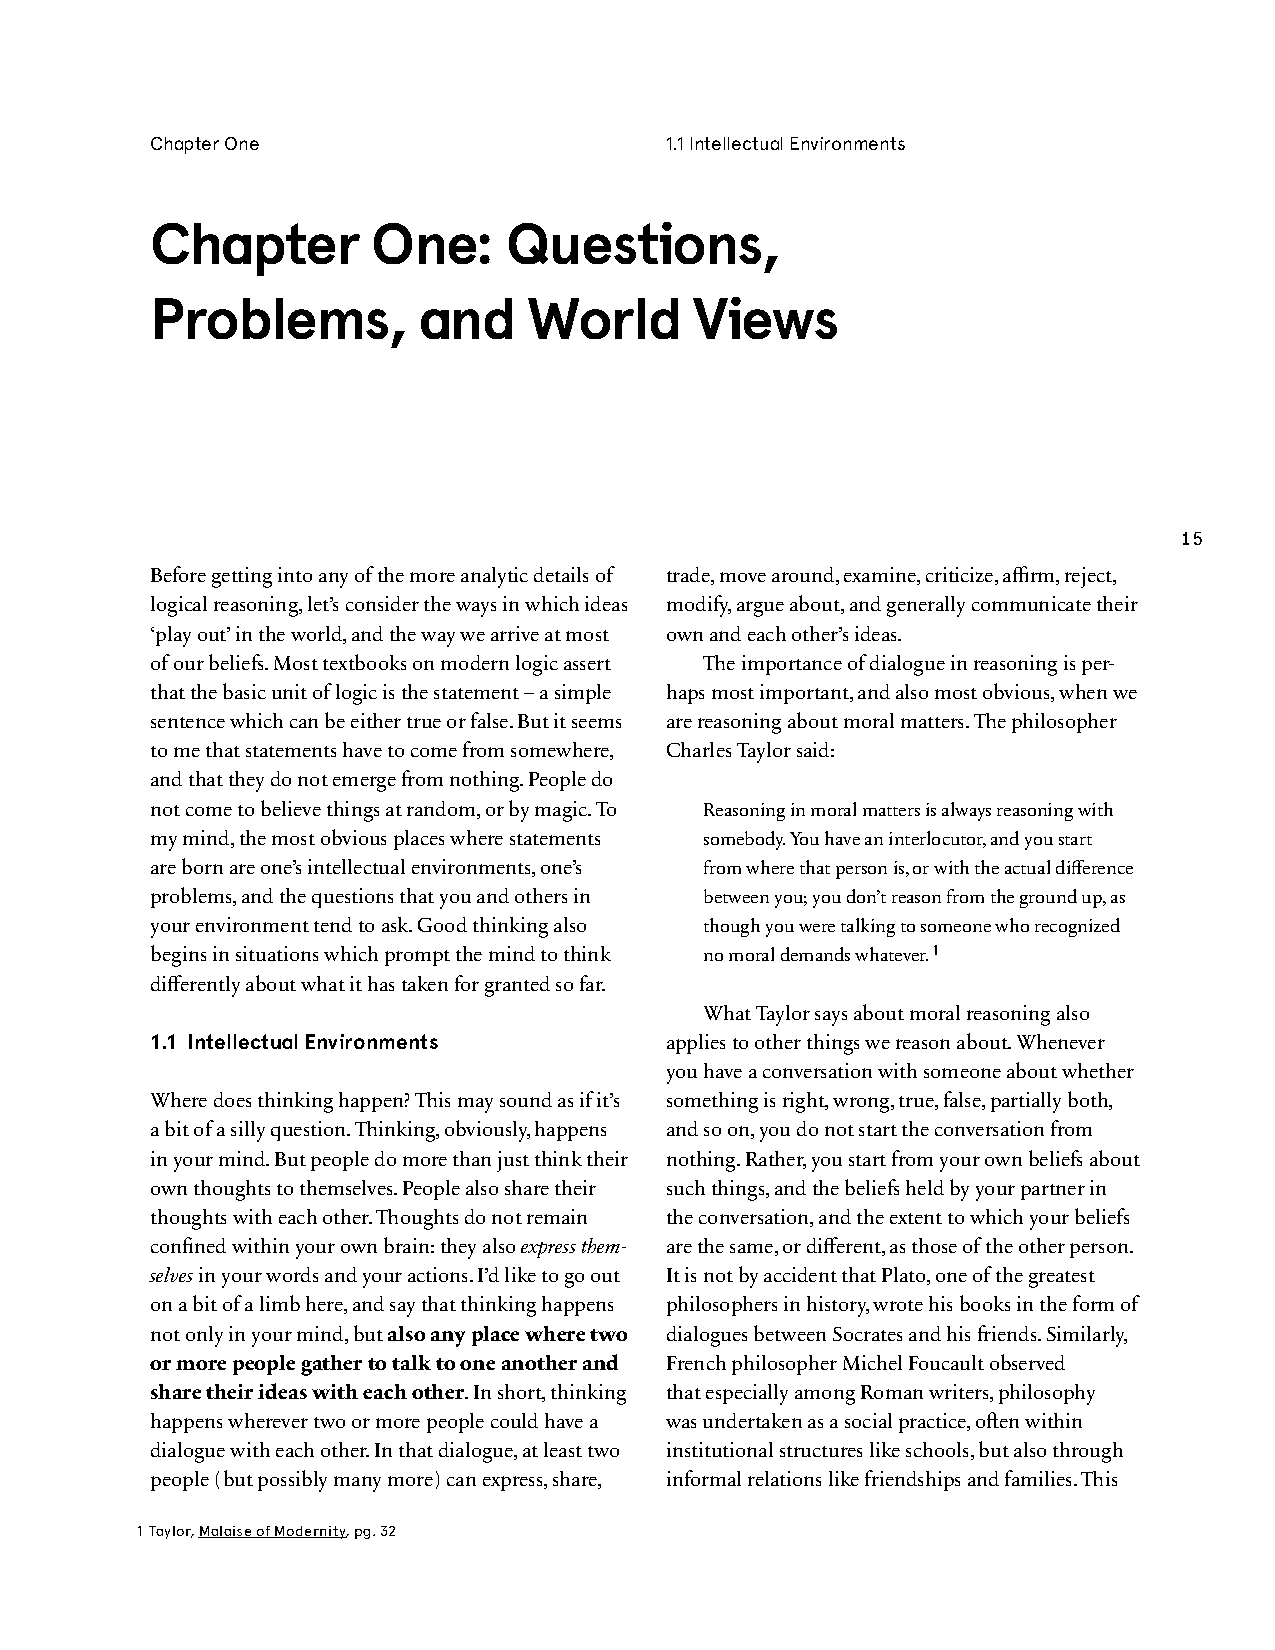
\includepdf[pages=-, pagecommand={}]{ch1-1.pdf}

\chapter{Habits of Good and Bad Thinking}
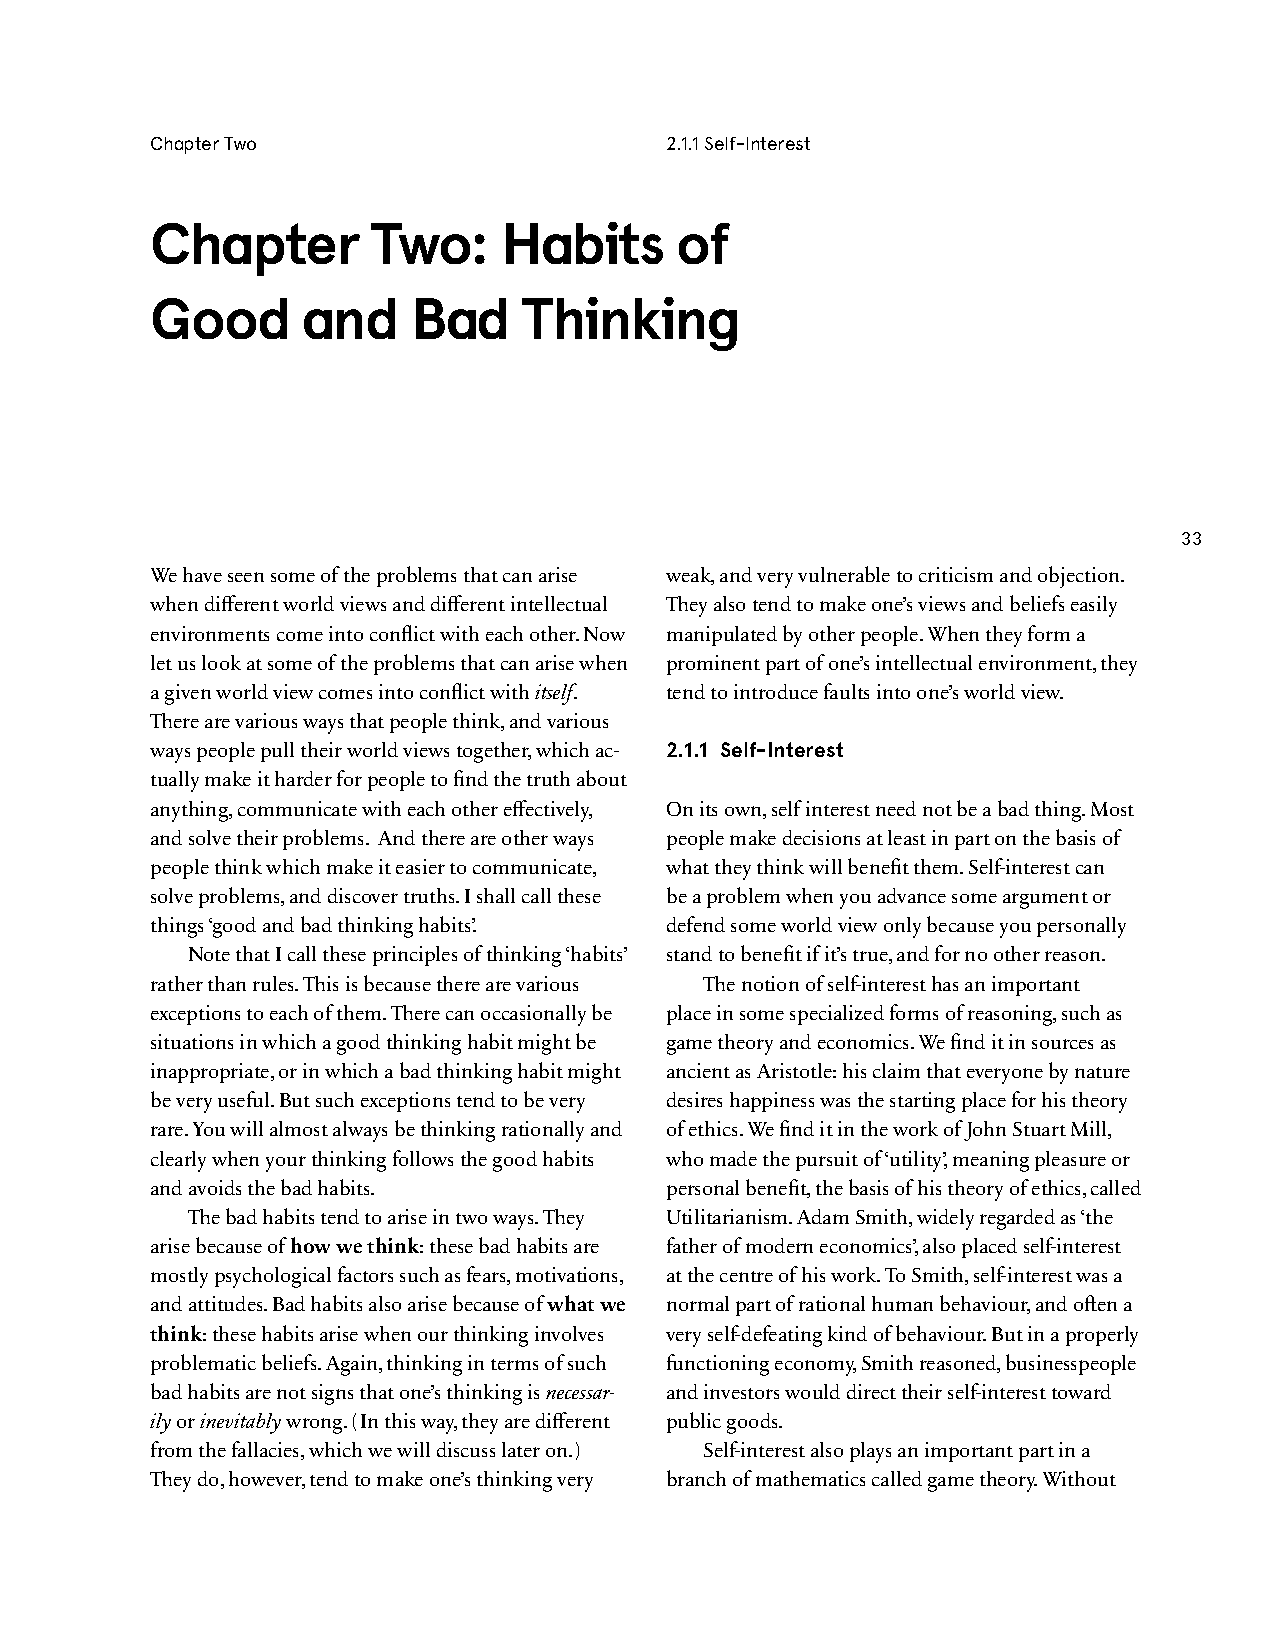
\includepdf[pages=-, pagecommand={}]{ch1-2.pdf}   
%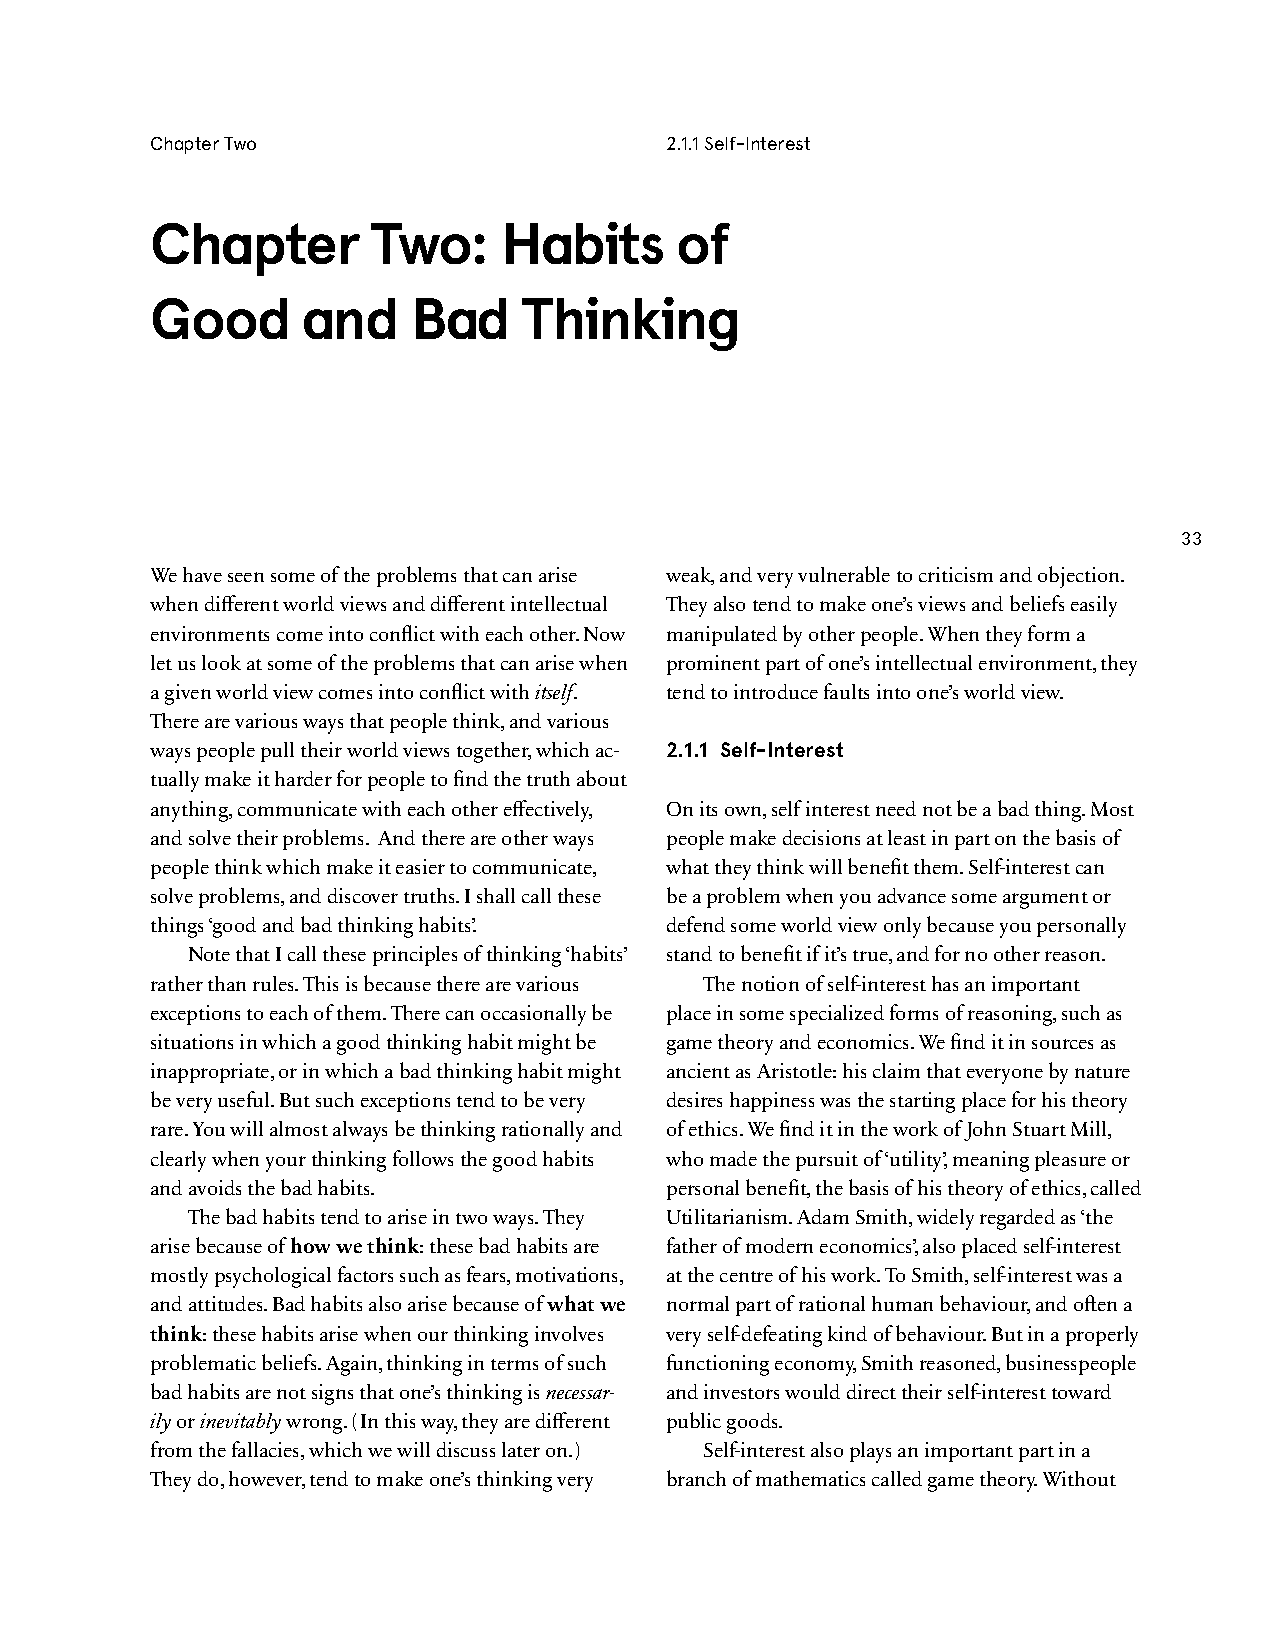
\includepdf[pages=-, pagecommand={}]{ch1-2.pdf}

%1
%\chapter{Chapter 3}
%mod2-1chapter 1 pages 1-20
\chapter{The Basics of Logical Analysis}

\subsection{What Is Logic?}
In Logic, the object of study is reasoning. This is an activity that humans engage in--when we
make claims and back them up with reasons, or when we make inferences about what follows from
a set of statements.

Like many human activities, reasoning can be done well, or it can be done badly. The goal of logic
is to distinguish good reasoning from bad. Good reasoning is not necessarily effective reasoning;
in fact, as we shall see, bad reasoning is pervasive and often extremely effective--in the sense that
people are often persuaded by it. In Logic, the standard of goodness is not effectiveness in the
sense of persuasiveness, but rather correctness according to logical rules.

In logic, we study the rules and techniques that allow us to distinguish good, correct reasoning
from bad, incorrect reasoning.

Since there is a variety of different types of reasoning, since it's possible to develop various
methods for evaluating each of those types, and since there are different views on what constitutes
correct reasoning, there are many approaches to the logical enterprise. We talk of logic, but also
of logics. A logic is just a set of rules and techniques for distinguishing good reasoning from bad.

So, the object of study in logic is human reasoning, with the goal of distinguishing the good from 
the bad. It is important to note that this approach sets logic apart from an alternative way of 
studying human reasoning, one more proper to a different discipline: psychology. It is possible to 
study human reasoning in a merely descriptive mode: to identify common patterns of reasoning and 
explore their psychological causes, for example. This is not logic. Logic takes up reasoning in a 
prescriptive mode: it tells how we ought to reason, not merely how we in fact typically 
do.\footnote{Psychologists have determined, for example, that most people are subject to what is 
called ``confirmation bias''--a tendency to seek out information to confirm one's pre-existing beliefs, 
and ignore contradictory evidence. There are lots of studies on this effect, including even 
brain-scans of people engaged in evaluating evidence. All of this is very interesting, but it's 
psychology, not logic; it's a mere descriptive study of reasoning. From a logical, prescriptive point 
of view, we simply say that people should try to avoid confirmation bias, because it can lead to bad 
reasoning.}

\subsection{Basic Notions: Propositions and Arguments} 
Reasoning involves claims or 
statements--making them and backing them up with reasons, drawing out their consequences. 
Propositions are the things we claim, state, assert. 

Propositions are the kinds of things that can be 
true or false. They are expressed by declarative sentences.\footnote{We distinguish propositions from 
the sentences that express them because a single proposition can be expressed by different sentences. 
`It's raining' and `Es regnet' both express the proposition that it's raining; one sentence does it 
in English, the other in German. Also, `John loves Mary' and `Mary is loved by John' both express the 
same proposition.} `This book is boring' is a declarative sentence; it expresses the proposition that 
this book is boring, which is (arguably) true (at least so far--but it's only the first page; wait 
until later, when things get exciting! 

Other kinds of sentences do not express propositions. Imperative sentences issue 
commands: `Sit down and shut up' is an imperative sentence; it doesn't make a claim, express 
something that might be true or false; either it's obeyed or it isn't. Interrogative sentences ask 
questions: `Who will win the World Cup this year?' is an interrogative sentence; it does not assert 
anything that might be true or false either.

Only declarative sentences express propositions, and so they are the only kinds of sentences we
will deal with at this stage of the study of logic. (More advanced logics have been developed to
deal with imperatives and questions, but we won't look at those in an introductory textbook.) \\

EXERCISES \\

Which of the following sentences are statements and which are not?

1.  No one understands me but you.

2.  Alligators are on average larger than crocodiles.

3.  Is an alligator a reptile or a mammal?

4.  An alligator is either a reptile or a mammal.

5.  Don't let any reptiles into the house.

6.  You may kill any reptile you see in the house.

7.  East Africans are not the best distance runners.

8.  Obama is not a Democrat.

9.  Some humans have wings.

10. Some things with wings cannot fly.

11. Was Obama born in Kenya or Hawaii?

12. Oh no! A grizzly bear!

13. Meet me in St Louis.

14. We met in St Louis yesterday.

15. I do not want to meet a grizzly bear in the wild.


The fundamental unit of reasoning is the argument. In logic, by `argument' we don't mean a
disagreement, a shouting match; rather, we define the term precisely:

\begin{quote}% probably needs \usepackage{csquotes}
\noindent
Argument = a set of propositions, one of which, the conclusion, is (supposed to be)
supported by the others, the premises.
\end{quote}

If we're reasoning by making claims and backing them up with reasons, then the claim that's being
backed up is the conclusion of an argument; the reasons given to support it are the argument's
premises. If we're reasoning by drawing an inference from a set of statements, then the inference
we draw is the conclusion of an argument, and the statements from which its drawn are the
premises.

We include the parenthetical hedge--``supposed to be''--in the definition to make room for bad
arguments. Remember, in Logic, we're evaluating reasoning. Arguments can be good or bad,
logically correct or incorrect. A bad argument, very roughly speaking, is one where the premises
fail to support the conclusion; a good argument's premises actually do support the conclusion.

To support the conclusion means, again very roughly, to give one good reasons for believing it.
This highlights the rhetorical purpose of arguments: we use arguments when we're disputing
controversial issues; they aim to persuade people, to convince them to believe their 
conclusion.\footnote{Reasoning in the sense of drawing inferences from a set of statements is a special case of this persuasive activity.
When we draw out reasonable conclusions from given information, we're convincing ourselves that we have good
reasons to believe them.}
As we said, in logic, we don't judge arguments based on whether or not they succeed in this goal--
there are logically bad arguments that are nevertheless quite persuasive. Rather, the logical
enterprise is to identify the kinds of reasons that ought to be persuasive (even if they sometimes
aren't).

\subsection{Recognizing and Explicating Arguments}
Before we get down to the business of evaluating arguments--deciding whether they're good or
bad--we need to develop some preliminary analytical skills. The first of these is, simply, the ability
to recognize arguments when we see them, and to figure out what the conclusion is (and what the
premises are).

What we want to learn first is how to explicate arguments. This involves writing down a bunch of
declarative sentences that express the propositions in the argument, and clearly marking which of
these sentences expresses the conclusion.

Let's start with a simple example. Here's an argument:

\begin{quote}
You really shouldn't eat at McDonald's. Why? First of all, they pay their workers very low
wages. Second, the animals that go into their products are raised in deplorable, inhumane
conditions. Third, the food is really bad for you. Finally, the burgers have poop in 
them.\footnote{I know, I know. But it's almost certainly true. Consumer Reports conducted a study in 2015, in which they tested
458 pounds of ground beef, purchased from 103 different stores in 26 different cities; all of the 458 pounds were
contaminated with fecal matter. This is because most commercial ground beef is produced at facilities that process
thousands of animals, and do it very quickly. The quickness ensures that sometimes -- 
rarely, but sometimes--a knifecut goes astray and the gastrointestinal tract is nicked, releasing poop. It gets cleaned up, but again, things are moving
fast, so they don't quite get all the poop. Now you've got one carcass -- again, out of hundreds or thousands --
contaminated with feces. But they make ground beef in a huge vat, with meat from all those carcasses mixed together.
So even one accident like this contaminates the whole batch. So yeah, those burgers -- basically all burgers, unless
you're grinding your own meat or sourcing your beef from a local farm -- have poop in them. Not much, but it's there.
Of course, it won't make you sick as long as you cook it right: 160 degrees F is enough to kill the poop-bacteria (E-coli, etc.),
so, you know, no big deal. Except for the knowledge that you're eating poop. Sorry.}
\end{quote}

The passage is clearly argumentative: its purpose is to convince you of something, namely, that
you shouldn't eat at McDonald's. That's the conclusion of the argument. The other claims are all
reasons for believing the conclusion--reasons for not eating at McDonald's. Those are the
premises.

To explicate the argument is simply to clearly identify the premises and the conclusion, by writing
down declarative sentences that express them. We would explicate the McDonald's argument like
this:

\begin{quote}
\noindent
McDonald's pays its workers very low wages. \\
The animals that go into their products are raised in deplorable, inhumane conditions. \\
McDonald's food is really bad for you. \\
\underline{Their burgers have poop in them}. \\
You shouldn't eat at McDonald's.
\end{quote}

We separate the conclusion from the premises with a horizontal line. Sometimes, you will see a special symbol
in front of the conclusion, which can be read as ``therefore.''

Speaking of `therefore', it's one of the words to look out for when identifying and explicating
arguments. Along with words like `consequently' and `thus', and phrases like `it follows that' and
`which implies that', it indicates the presence of the conclusion of an argument. Similarly, words
like `because', `since', and `for' indicate the presence of premises.\\


%\begin{table}[A list of some common premise and conclusion indicators]
\begin{table}[htp]
\begin{tabular}{|l|l|}
\hline
\textbf{Premise Indicators}        & \textbf{Conclusion indicators} \\
\hline
since                     & therefore             \\
because                   & so                    \\
for                       & hence                 \\
as                        & thus                  \\
given that                & implies that          \\
seeing that               & consequently          \\
for the reason that       & it follows that       \\
is shown by the fact that & we may conclude that \\
\hline
\end{tabular}
\end{table}

We should also note that it is possible for a single sentence to express more than one proposition.
If we added this sentence to our argument--`McDonald's advertising targets children to try to
create lifetime addicts to their high-calorie foods, and their expansion into global markets has
disrupted native food distribution systems, harming family farmers'--we would write down two
separate declarative sentences in our explication, expressing the two propositions asserted in the
sentence--about children and international farmers, respectively. Indeed, it's possible for a single
sentence to express an entire argument. `You shouldn't eat at McDonald's because they're a bad
corporate actor' gives you a conclusion and a premise at once. An explication would merely
separate them.

\subsubsection{Paraphrasing}
The argument about McDonald's was an easy case. It didn't have a word like `therefore' to tip us
off to the presence of the conclusion, but it was pretty clear what the conclusion was anyway. All
we had to do was ask ourselves, ``What is this person trying to convince me to believe?'' The
answer to that question is the conclusion of the argument.

Another way the McDonald's argument was easy: all of the sentences were declarative sentences,
so when we explicated the argument, all we had to do was write them down. But sometimes
argumentative passages aren't so cooperative. Sometimes they contain non-declarative sentences.
Recall, arguments are sets of propositions, and only declarative sentences express propositions; so
if an argumentative passage contains non-declarative sentences (questions, commands, etc.), we
need to change their wording when we explicate the argument, turning them into declarative
sentences that express a proposition. This is called paraphrasing.

Suppose, for example, that the McDonald's argument were exactly as originally presented, except
the first sentence were imperative, not declarative:

\begin{quote}
Don't eat at McDonald's. Why? First of all, they pay their workers very low wages.
Second, the animals that go into their products are raised in deplorable, inhumane
conditions. Third, the food is really bad for you. Finally, the burgers have poop in them.
\end{quote}

We just switched from `You shouldn't eat at McDonald's' to `Don't eat at McDonald's.' But it
makes a difference. The first sentence is declarative; it makes a claim about how things are
(morally, with respect to your obligations in some sense): you shouldn't do such-and-such. It's
possible to disagree with the claim: Sure I should, and so should everybody else; their fries are
delicious! `Don't eat at McDonald's', on the other hand, is not like that. It's a command. It's
possible to disobey it, but not to disagree with it; imperative sentences don't make claims about
how things are, don't express propositions.

Still, the passage is clearly argumentative: the purpose remains to persuade the listener not to eat
at McDonald's. We just have to be careful, when we explicate the argument, to paraphrase the first
sentence--to change its wording so that it becomes a declarative, proposition-expressing sentence.
`You shouldn't eat at McDonald's' works just fine.

Let's consider a different example:

\begin{quote}
\noindent
I can't believe anyone would support a \$15 per hour minimum wage. Don't they realize
that it would lead to massive job losses? And the strain such a policy would put on small
businesses could lead to an economic recession.
\end{quote}

The passage is clearly argumentative: this person is engaged in a dispute about a controversial
issue--the minimum wage--and is staking out a position and backing it up. What is that position?
Apparently, this person opposes the idea of raising the minimum wage to \$15.

There are two problems we face in explicating this argument. First, one of the sentences in the
passage--the second one--is non-declarative: it's an interrogative sentence, a question.
Nevertheless, it's being used in this passage to express one of the person's reasons for opposing
the minimum wage increase--that it would lead to job losses. So we need to paraphrase,
transforming the interrogative into a declarative--something like `A \$15 minimum wage would
lead to massive job losses'.

The other problem is that the first sentence, while a perfectly respectable declarative sentence,
can't be used as-is in our explication. For while it's clearly being used by to express this person's
main point, the conclusion of his argument against the minimum wage increase, it does so
indirectly. What the sentence literally and directly expresses is not a claim about the wisdom of
the minimum wage increase, but rather a claim about the speaker's personal beliefs: `I can't believe
anyone would support a \$15 per hour minimum wage'. But that claim isn't the conclusion of the
argument. The speaker isn't trying to convince people that he believes (or can't believe) a certain
thing; he's trying to convince them to believe the same thing he believes, namely, that raising the
minimum wage to \$15 is a bad idea. So, despite the first sentence being a declarative, we still have
to paraphrase it. It expresses a proposition, but not the conclusion of the argument.

Our explication of the argument would look like this:

\begin{quote}
\noindent

Increasing the minimum wage to \$15 per hour would lead to massive job losses. \\
\underline{The policy would put a strain on small businesses that might lead to a recession.} \\
/ Increasing the minimum wage to \$15 per hour is a bad idea. \\
\end{quote}

EXERCISES \\

Which of the following are arguments?           
If it is an argument,
identify the conclusion of the argument.

1. The woman in the hat is not a witch since witches have long noses and
    she doesn't have a long nose.

2. I have been wrangling cattle since before you were old enough to tie
    your own shoes.

3. Albert is angry with me so he probably won't be willing to help me wash
    the dishes.

4. First I washed the dishes and then I dried them.

5. If the road wasn't icy, the car wouldn't have slid off the turn.

6. Albert isn't a fireman and he isn't a fisherman either.

7. Are you seeing that rhinoceros over there? It is huge!

8. The fact that obesity has become a problem in the U.S. is shown by the
    fact that obesity rates have risen significantly over the past four decades.

9. Bob showed me a graph with the rising obesity rates and I was very
    surprised to see how much they've risen.

10. Albert isn't a fireman because Albert is a Greyhound, which is a kind of
    dog, and dogs can't be firemen.

11. Charlie and Violet are dogs and since dogs dont sweat, it is obvious that
    Charlie and Violet don't sweat.

12. The reason I forgot to lock the door is that I was distracted by the clown
    riding a unicycle down our street while singing Lynyrd Skynyrd's ``Simple
    Man."

13. What Bob told you is not the real reason that he missed his plane to
    Denver.

14. Samsung stole some of Apple's patents for their smartphones, so Apple
    stole some of Samsung's patents back in retaliation.

15. No one who has ever gotten frostbite while climbing K2 has survived to
    tell about it, therefore no one ever will.






\subsubsection{Enthymemes: Tacit Propositions}
So sometimes, when we explicate an argument, we have to take what's present in the
argumentative passage and change it slightly, so that all of the sentences we write down express
the propositions that are in the argument. This is paraphrasing. Other times, we have to do even
more: occasionally, we have to fill in missing propositions; argumentative passages might not state
all of the propositions in an argument explicitly, and in the course of explicating their arguments,
we have to make these implicit, tacit propositions explicit by writing down the appropriate
declarative sentences.

There's a fancy Greek word for argumentative passages that leave certain propositions unstated:
enthymemes. Here's an example:

\begin{quote}
Hillary Clinton has more experience in public office than Donald Trump; she has a much
deeper knowledge of the issues; she's the only one with the proper temperament to lead
our country. I rest my case.
\end{quote}

Again, the argumentative intentions here are plain: this person is staking out a position on a
controversial topic--a presidential election. But notice, that position--that one should prefer
Clinton to Trump--is never stated explicitly. We get reasons for having that preference--the
premises of the argument are explicit--but we never get a statement of the conclusion. But since
this is clearly the upshot of the passage, we need to include a sentence expressing it in our
explication:

\begin{quote}
Clinton has more experience than Trump. \\
Clinton has deeper knowledge of issues than Trump. \\
Clinton has the proper temperament to lead the country, while Trump does not. \\
/ One should prefer Clinton to Trump in the presidential election. \\
\end{quote}

In that example, the conclusion of the argument was tacit. Sometimes, premises are unstated and
we should make them explicit in our explication of the argument. Now consider this passage:

\begin{quote}
The sad fact is that wages for middle-class workers have stagnated over the past several
decades. We need a resurgence of the union movement in this country.
\end{quote}

This person is arguing in favor of labor unions; the second sentence is the conclusion of the
argument. The first sentence gives the only explicit premise: the stagnation of middle-class wages.
But notice what the passage doesn't say: what connection there might be between the two things.
What do unions have to do with middle-class wages?

There's an implicit premise lurking in the background here--something that hasn't been said, but
which needs to be true for the argument to go through. We need a claim that connects the premise
to the conclusion--that bridges the gap between them. Something like this: A resurgence of unions
would lead to wage growth for middle-class workers. The first sentence identifies a problem; the
second sentence purports to give a solution to the problem. But it's only a solution if the tacit
premise we've uncovered is true. If unions don't help raise middle-class wages, then the argument
falls apart.

This is the mark of the kinds of tacit premises we want to uncover: if they're false, they undermine
the argument. Often, premises like this are unstated for a reason: they're controversial claims on
their own, requiring a lot of evidence to support them; so the arguer leaves them out, preferring
not to get bogged down. When we draw them out, however, we can force a more robust dialectical
exchange, focusing the argument on the heart of the matter. In this case, a discussion about the
connection between unions and middle-class wages would be in order. There's a lot to be said on
that topic.

\subsubsection{Arguments v Explanations}
One final item on the topic of ``Recognizing and Explicating Arguments.'' We've been focusing
on explication; this is a remark about the recognition side. Some passages may superficially
resemble arguments--they may, for example, contain words like `therefore' and `because', which
normally indicate conclusions and premises in argumentative passages--but which are
nevertheless not argumentative. Instead, they are explanations.

Consider this passage:

\begin{quote}
Because female authors of her time were often stereotyped as writing light-hearted
romances, and because her real name was well-known for other (sometimes scandalous)
reasons, Mary Ann Evans was reluctant to use her own name for her novels. She wanted
her work to be taken seriously and judged on its own merits. Therefore, she adopted the
pen name `George Eliot'.
\end{quote}

This passage has the words `because' (twice), and `therefore', which typically indicate the
presence of premises and a conclusion, respectively. But it is not an argument. It's not an argument
because it does not have the rhetorical purpose of an argument: the aim of the passage is not to
convince you of something. If it were an argument, the conclusion would be the claim following
`therefore', namely, the proposition that Mary Ann Evans adopted the pen name `George Eliot'.
But this claim is not the conclusion of an argument; the passage is not trying to persuade us to
believe that Evans adopted a pen name. That she did so is not a controversial claim. Rather, that's
a fact that's assumed to be known already. The aim of the passage is to explain to us why Evans
made that choice. The rhetorical purpose is not to convince; it is to inform, to edify. The passage
is an explanation, not an argument.

So, to determine whether a given passage is an argument or an explanation, we need to figure out
its rhetorical purpose. Why is the author saying these things to me? Is she trying to convince me
of something, or is she merely trying to inform me--to give me an explanation for something I
already knew? Sometimes this is easy, as with the George Eliot passage; it's hard to imagine
someone saying those things with persuasive intent. Other times, however, it's not so easy.
Consider the following:

Many of the celebratory rituals (of Christmas), as well as the timing of the holiday, have
their origins outside of, and may predate, the Christian commemoration of the birth of
Jesus. Those traditions, at their best, have much to do with celebrating human relationships
and the enjoyment that this life has to offer. As an atheist, I have no hesitation in embracing
the holiday and joining with believers and nonbelievers alike to celebrate what we have in
common.\footnote{John Teehan, 12/24/2006, ``A Holiday Season for Atheists, Too,'' The New York 
Times. Excerpted in Copi and Cohen,
2009, Introduction to Logic 13e, p. 25.}

Unless we understand a little bit more about the context of this passage, it's difficult to determine
the speaker's intentions. It may appear to be an argument. That atheists should embrace a religious
holiday like Christmas is, among many, a controversial claim. Controversial claims are the kinds
of claims that we often try to convince skeptical people to believe. If the speaker's audience for
this passage is a bunch of hard-line atheists, who vehemently reject anything with a whiff of
religiosity, who consider Christmas a humbug, then it's pretty clear that the speaker is trying to
offer reasons for them to reconsider their stance; he's trying to convince them to embrace
Christmas; he's making an argument. If we explicated the argument, we would paraphrase the last
sentence to represent the controversial conclusion: `Atheists should have no hesitation embracing
and celebrating Christmas'.

But in a different context, with a different audience, this may not be an argument. If we leave the
claim in the final sentence as-is--`As an atheist, I have no hesitation in embracing the holiday and
joining with believers and nonbelievers alike to celebrate what we have in common'--we have a
claim about the speaker's personal beliefs and inclinations. Typically, as we saw above, such
claims are not suitable as the conclusions of arguments; we don't usually spend time trying to
convince people that we believe such-and-such. But what is more typical is providing people with
explanations for why we believe things. If the author of our passage is an atheist, and he's saying
these things to friends of his, say, who know he's an atheist, we might have just such an
explanation. His friends know he's not religious, but they know he loves Christmas. That's kind
of weird. Don't atheists hate religious holidays? Not so, says our speaker. Let me explain to you
why I have no problems with Christmas, despite my atheism.
Again, the difference between arguments and explanations comes down to rhetorical purpose:
arguments try to convince people; explanations try to inform them. Determining whether a given
passage is one or the other involves figuring out the author's intentions. To do this, we must
carefully consider the context of the passage. \\

EXERCISES \\

1. Identify the conclusions in the following arguments.

(a) Every citizen has a right--nay, a duty--to defend himself and his family. This is all
the more important in these increasingly dangerous times. The framers of the Constitution,
in their wisdom, enshrined the right to bear arms in that very document. We should all
oppose efforts to restrict access to guns.

(b) Totino's pizza rolls are the perfect food. They have all the great flavor of pizza, with
the added benefit of portability!

(c) Because they go overboard making things user-friendly, Apple phones are inferior to
those with Android operating systems. If you want to change the default settings on an
Apple phone to customize it to your personal preferences, it's practically impossible to
figure out how. The interface is so dumbed down to appeal to the ``average consumer'' that
it's super hard to find where the controls for advanced settings even are. On Android
phones, though, everything's right there in the open.

(d) The U.S. incarcerates more people per capita than any other country on Earth, many
for non-violent drug offenses. Militarized policing of our inner cities has led to scores of
unnecessary deaths and a breakdown of trust between law enforcement and the
communities they are supposed to serve and protect. We need to end the ``War on Drugs''
now. Our criminal justice system is broken. The War on Drugs broke it.

(e) The point of a watch is to tell you what time it is. Period. Rolexes are a complete waste
of money. They don't do any better at telling the time, and they cost a ton!

2. Explicate the following arguments, paraphrasing as necessary.

(a) You think that if the victims of the mass shooting had been armed that would've made
things better? Are you nuts? The shooting took place in a bar; not even the NRA thinks it's
a good idea to allow people to carry guns in a drinking establishment. And don't be fooled
by the fantasy that ``good guys with guns'' would prevent mass murder. More likely, the
situation would've been even bloodier, with panicked people shooting randomly all over
the place.

(b) The heat will escape the house through the open door, which means the heater will
keep running, which will make our power bill go through the roof. Then we'll be broke.
So stop leaving the door open when you come into the house.

(c) Do you like delicious food? How about fun games? And I know you like cool prizes.
Well then, Chuck E. Cheese's is the place for you.

3. Write down the tacit premises that the following arguments depend on for their success.

(a) Cockfighting is an exciting pastime enjoyed by many people. It should therefore be
legal.

(b) The president doesn't understand the threat we face. He won't even use the phrase
``Radical Islamic Terror.''

4. Write down the tacit conclusion that follows most immediately from the following.

(a) If there really were an all-loving God looking down on us, then there wouldn't be so
much death and destruction visited upon innocent people.

(b) The death penalty is immoral. Numerous studies have shown that there is racial bias in
its application. The rise of DNA testing has exonerated scores of inmates on death row;
who knows how many innocent people have been killed in the past? The death penalty is
also impractical. Revenge is counterproductive: ``An eye for an eye leaves the whole world
blind,'' as Gandhi said. Moreover, the costs of litigating death penalty cases, with their
endless appeals, are enormous. The correct decision for policymakers is clear.

5. Decide whether the following are arguments or explanations, given their context. If the passage
is an argument, write down its conclusion; if it is an explanation, write down the fact that is being
explained.

(a) Michael Jordan is the best of all time. I don't care if Kareem scored more points; I
don't care if Russell won more championships. The simple fact is that no other player in
history displayed the stunning combination of athleticism, competitive drive, work ethic,
and sheer jaw-dropping artistry of Michael Jordan. (Context: Sports talk radio host going
on a ``rant'')

(b) Because different wavelengths of light travel at different velocities when they pass
through water droplets, they are refracted at different angles. Because these different
wavelengths correspond to different colors, we see the colors separated. Therefore, if the
conditions are right, rainbows appear when the sun shines through the rain. (Context: grade
school science textbook)

(c) The primary motivation for the Confederate States in the Civil War was not so much
the preservation of the institution of slavery, but the preservation of the sovereignty of
individual states guaranteed by the 10th Amendment to the U.S. Constitution. Southerners
of the time were not the simple-minded racists they were often depicted to be. Leaders in
the southern states were disturbed by the over-reach of the Federal government into issues
of policy more properly decided by the states. That slavery was one of those issues is
incidental. (Context: excerpt from Rebels with a Cause: An Alternative History of the Civil
War)

(d) This is how natural selection works: those species with traits that promote reproduction
tend to have an advantage over competitors and survive; those without such traits tend to
die off. The way that humans reproduce is by having sex. Since the human species has
survived, it must have traits that encourage reproduction--that encourage having sex. This
is why sex feels good. Sex feels good because if it didn't, the species would not have
survived. (Context: excerpt from \emph{Evolutionary Biology for Dummies})

\subsection{Deductive and Inductive Arguments}

As we noted earlier, there are different logics--different approaches to distinguishing good
arguments from bad ones. One of the reasons we need different logics is that there are different
kinds of arguments. In this section, we distinguish two types: deductive and inductive arguments.

\begin{quote}
Sally Johansson does all her grocery shopping at an organic food co-op. She's a huge fan
of tofu. She's really into those week-long juice cleanse thingies. And she's an active
member of PETA. I conclude that she's a vegetarian.

(a) Make up a new piece of information about Sally that weakens the argument.

(b) Make up a new piece of information about Sally that strengthens the argument.
\end{quote}

\subsection{Diagramming Arguments}
Before we get down to the business of evaluating arguments--of judging them valid or invalid,
strong or weak--we still need to do some preliminary work. We need to develop our analytical
skills to gain a deeper understanding of how arguments are constructed, how they hang together.
So far, we've said that the premises are there to support the conclusion. But we've done very little
in the way of analyzing the structure of arguments: we've just separated the premises from the
conclusion. We know that the premises are supposed to support the conclusion. What we haven't
explored is the question of just how the premises in a given argument do that job--how they work
together to support the conclusion, what kinds of relationships they have with one another. This is
a deeper level of analysis than merely distinguishing the premises from the conclusion; it will
require a mode of presentation more elaborate than a list of propositions with the bottom one
separated from the others by a horizontal line. To display our understanding of the relationships
among premises supporting the conclusion, we are going to depict them: we are going to draw
diagrams of arguments.

Here's how the diagrams will work. They will consist of three elements: (1) circles with numbers
inside them--each of the propositions in the argument we're diagramming will be assigned a
number, so these circled numbers in the diagram will represent the propositions; (2) arrows pointed
at circled numbers--these will represent relationships of support, where one or more propositions
provide a reason for believing the one pointed to; and (3) horizontal brackets--propositions
connected by these will be interdependent (in a sense to be specified below).

Our diagrams will always feature the circled number corresponding to the conclusion at the
bottom. The premises will be above, with brackets and arrows indicating how they collectively
support the conclusion and how they're related to one another. There are a number of different
relationships that premises can have to one another. We will learn how to draw diagrams of
arguments by considering them in turn.

\subsubsection{Independent Premises}

Often, different premises will support a conclusion--or another premise--individually, without
help from any others. When this is the case, we draw an arrow from the circled number
representing that premise to the circled number representing the proposition it supports.

Consider this simple argument:

\begin{quote}
(1) Marijuana is less addictive than alcohol. In addition, (2) it can be used as a medicine to
treat a variety of conditions. Therefore, (3) marijuana should be legal.
\end{quote}

The last proposition is clearly the conclusion (the word `therefore' is a big clue), and the first two
propositions are the premises supporting it. They support the conclusion independently. The mark
of independence is this: each of the premises would still provide support for the conclusion even
if the other weren't true; each, on its own, gives you a reason for believing the conclusion. In this
case, then, we diagram the argument as follows: \\

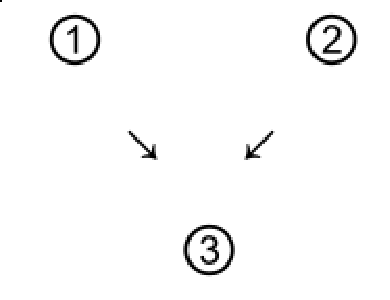
\includegraphics[scale=.49]{diagram1.pdf}
%%%%%%%%%%%
%%%%%%%%%%% pg 19 first one
%%%%%%%%%%%


\subsubsection{Intermediate Premises}
Some premises support their conclusions more directly than others. Premises provide more indirect
support for a conclusion by providing a reason to believe another premise that supports the
conclusion more directly. That is, some premises are intermediate between the conclusion and
other premises.

Consider this simple argument:

(1) Automatic weapons should be illegal. (2) They can be used to kill large numbers of
people in a short amount of time. This is because (3) all you have to do is hold down the
trigger and bullets come flying out in rapid succession.

The conclusion of this argument is the first proposition, so the premises are propositions 2 and 3.
Notice, though, that there's a relationship between those two claims. The third sentence starts with
the phrase `This is because', indicating that it provides a reason for another claim. The other claim
is proposition 2; `This' refers to the claim that automatic weapons can kill large numbers of people
quickly. Why should I believe that they can do that? Because all one has to do is hold down the
trigger to release lots of bullets really fast. Proposition 2 provides immediate support for the
conclusion (automatic weapons can kill lots of people really quickly, so we should make them
illegal); proposition 3 supports the conclusion more indirectly, by giving support to proposition 2.
Here is how we diagram in this case: \\

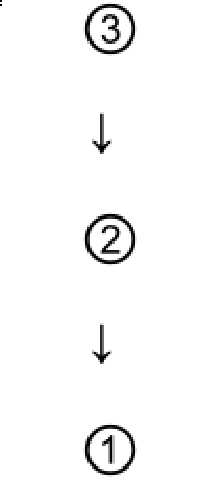
\includegraphics[scale=.49]{diagram2.pdf}
%%%%%%%%%%%%%%%
%%%%%%%%%%%%%%% pg 19 second one
%%%%%%%%%%%%%%%


\subsubsection{Joint Premises}
Sometimes premises need each other: the job of supporting another proposition can't be done by
each on its own; they can only provide support together, jointly. Far from being independent, such
premises are interdependent. In this situation, on our diagrams, we join together the interdependent
premises with a bracket underneath their circled numbers.

There are a number of different ways in which premises can provide joint support. Sometimes,
premises just fit together like a hand in a glove; or, switching metaphors, one premise is like the
key that fits into the other to unlock the proposition they jointly support. An example can make
this clear:

\begin{quote}
(1) The chef has decided that either salmon or chicken will be tonight's special. (2) Salmon
won't be the special. Therefore, (3) the special will be chicken.
\end{quote}

Neither premise 1 nor premise 2 can support the conclusion on its own. A useful rule of thumb for
checking whether one proposition can support another is this: read the first proposition, then say
the word `therefore', then read the second proposition; if it doesn't make any sense, then you can't
draw an arrow from the one to the other. Let's try it here: ``The chef has decided that either salmon
or chicken will be tonight's special; therefore, the special will be chicken.'' That doesn't make any
sense. What happened to salmon? Proposition 1 can't support the conclusion on its own. Neither
can the second: ``Salmon won't be the special; therefore, the special will be chicken.'' Again, that
makes no sense. Why chicken? What about steak, or lobster? The second proposition can't support
the conclusion on its own, either; it needs help from the first proposition, which tells us that if it's
not salmon, it's chicken. Propositions 1 and 2 need each other; they support the conclusion jointly.
This is how we diagram the argument: \\

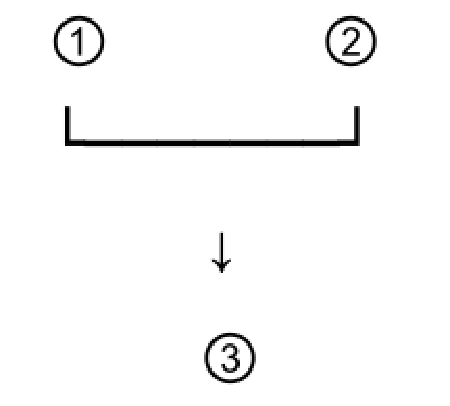
\includegraphics[scale=.49]{diagram3.pdf}
%%%%%%%%%%%%%%%%%%%
%%%%%%%%%%%%%%%%%%% page 20
%%%%%%%%%%%%%%%%%%%

The same diagram would depict the following argument:

\begin{quote}
(1) John Le Carr\'e gives us realistic, three-dimensional characters and complex, interesting
plots. (2) Ian Fleming, on the other hand, presents an unrealistically glamorous picture of
international espionage, and his plotting isn't what you'd call immersive. (3) Le Carr\'e is a
better author of spy novels than Fleming.
\end{quote}

In this example, the premises work jointly in a different way than in the previous example. Rather
than fitting together hand-in-glove, these premises each give us half of what we need to arrive at
the conclusion. The conclusion is a comparison between two authors. Each of the premises makes
claims about one of the two authors. Neither one, on its own, can support the comparison, because
the comparison is a claim about both of them. The premises can only support the conclusion
together. We would diagram this argument the same way as the last one.

Another common pattern for joint premises is when general propositions need help to provide
support for particular propositions. Consider the following argument:

(1) People shouldn't vote for racist, incompetent candidates for president. (2) Donald Trump
seems to make a new racist remark at least twice a week. And (3) he lacks the competence
to run even his own (failed) businesses, let alone the whole country. (4) You shouldn't vote
for Trump to be the president.

The conclusion of the argument, the thing it's trying to convince us of, is the last proposition--
you shouldn't vote for Trump. This is a particular claim: it's a claim about an individual person,
Trump. The first proposition in the argument, on the other hand, is a general claim: it asserts that,
generally speaking, people shouldn't vote for incompetent racists; it makes no mention of an
individual candidate. It cannot, therefore, support the particular conclusion--about Trump--on its
own. It needs help from other particular claims--propositions 2 and 3--that tell us that the
individual in the conclusion, Trump, meets the conditions laid out in the general proposition 1:
racism and incompetence. This is how we diagram the argument: \\

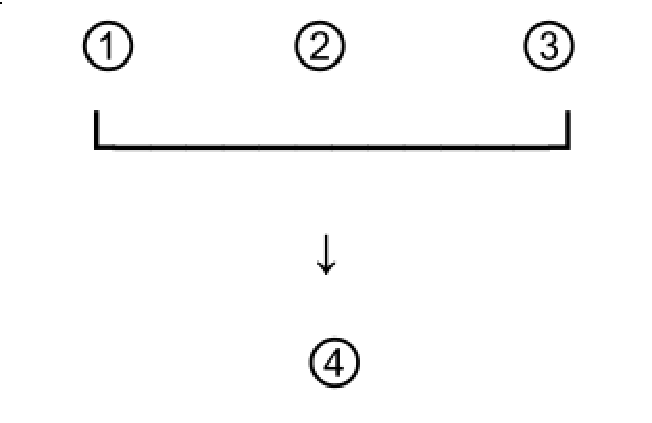
\includegraphics[scale=.49]{diagram4.pdf}
%%%%%%%%%%%%%%%
%%%%%%%%%%%%%%% pg 21
%%%%%%%%%%%%%%%


Occasionally, an argumentative passage will only explicitly state one of a set of joint premises
because the others ``go without saying''--they are part of the body of background information
about which both speaker and audience agree. In the last example, that Trump was an incompetent
racist was not uncontroversial background information. But consider this argument:

\begin{quote}
(1) It would be good for the country to have a woman with lots of experience in public
office as president. (2) People should vote for Hillary Clinton.
\end{quote}

Diagramming this argument seems straightforward: an arrow pointing from (1) to (2) But we've
got the same relationship between the premise and conclusion as in the last example: the premise
is a general claim, mentioning no individual at all, while the conclusion is a particular claim about
Hillary Clinton. Doesn't the general premise ``need help'' from particular claims to the effect that
the individual in question, Hillary Clinton, meets the conditions set forth in the premise--i.e., that
she's a woman and that she has lots of experience in public office? No, not really. Everybody
knows those things about her already; they go without saying, and can therefore be left unstated
(implicit, tacit).

But suppose we had included those obvious truths about Clinton in our presentation of the
argument; suppose we had made the tacit premises explicit:

\begin{quote}
(1) It would be good for the country to have a woman with lots of experience in public
office as president. (2) Hillary Clinton is a woman. And (3) she has deep experience with
public offices--as a First Lady, U.S. Senator, and Secretary of State. (4) People should vote
for Hillary Clinton.
\end{quote}

How do we diagram this? Earlier, we talked about a rule of thumb for determining whether or not
it's a good idea to draw an arrow from one number to another in a diagram: read the sentence
corresponding to the first number, say the word `therefore', then read the sentence corresponding
to the second number; if it doesn't make sense, then the arrow is a bad idea. But if it does make
sense, does that mean you should draw the arrow? Not necessarily. Consider the first and last
sentences in this passage. Read the first, then `therefore', then the last. Makes pretty good sense!
That's just the original formulation of the argument with the tacit propositions remaining implicit.
And in that case we said it would be OK to draw an arrow from the general premise's number
straight to the conclusion's. But when we add the tacit premises--the second and third sentences
in this passage--we can't draw an arrow directly from (1) to (4) To do so would obscure the
relationship among the first three propositions and misrepresent how the argument works. If we
drew an arrow from (1) to (4) what would we do with (2) to (3) in our diagram? Do they get their
own arrows, too? No, that won't do. Such a diagram would be telling us that the first three
propositions each independently provide a reason for the conclusion. But they're clearly not
independent; there's a relationship among them that our diagram must capture, and it's the same
relationship we saw in the parallel argument about Trump, with the particular claims in the second
and third propositions working together with the general claim in the first: \\


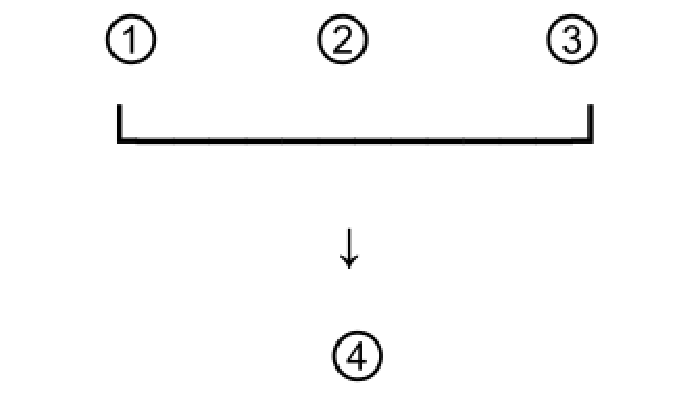
\includegraphics[scale=.49]{diagram5.pdf}
%%%%%%%%%%%%%%%
%%%%%%%%%%%%%%% same as on 21
%%%%%%%%%%%%%%%

The arguments we've looked at thus far have been quite short--only two or three premises. But of
course some arguments are longer than that. Some are much longer. The system of mapping generalizes 
to these longer arguments. In future lessons, we'll start to look at arguments with more and more 
premises.


EXERCISES \\

Diagram the following arguments.

\begin{enumerate}
\item (1) Hillary Clinton would make a better president than Donald Trump. (2) Clinton is a toughminded pragmatist who gets things done. (3) Trump is a thin-skinned maniac who will be totally
ineffective in dealing with Congress.

\item (1) Donald Trump is a jerk who's always offending people. Furthermore, (2) he has no
experience whatsoever in government. (3) Nobody should vote for him to be president.

\item (1) Human beings evolved to eat meat, so (2) eating meat is not immoral. (3) It's never immoral
for a creature to act according to its evolutionary instincts.

\item (1) We need new campaign finance laws in this country. (2) The influence of Wall Street money
on elections is causing a breakdown in our democracy with bad consequences for social justice.
(3) Politicians who have taken those donations are effectively bought and paid for, consistently
favoring policies that benefit the rich at the expense of the vast majority of citizens.

\item (1) Voters shouldn't trust any politician who took money from Wall Street bankers. (2) Hillary
Clinton accepted hundreds of thousands of dollars in speaking fee from Goldman Sachs, a big
Wall Street firm. (3) You shouldn't trust her.

\item (1) There are only three possible explanations for the presence of the gun at the crime scene:
either the defendant just happened to hide from the police right next to where the gun was found,
or the police planted the gun there after the fact, or it was really the defendant's gun like the
prosecution says. (2) The first option is too crazy a coincidence to be at all believable, and (3) we've
been given no evidence at all that the officers on the scene had any means or motivation to plant
the weapon. Therefore, (4) it has to be the defendant's gun.

\item (1) Golden State has to be considered the clear favorite to win the NBA Championship. (2) No
team has ever lost in the Finals after taking a 3-games-to-1 lead, and (3) Golden State now leads
Cleveland 3-to-1. In addition, (4) Golden State has the MVP of the league, Stephen Curry.

\item (1) We should increase funding to public colleges and universities. First of all, (2) as funding
has decreased, students have had to shoulder a larger share of the financial burden of attending
college, amassing huge amounts of debt. (3) A recent report shows that the average college student
graduates with almost \$30,000 in debt. Second, (4) funding public universities is a good
investment. (5) Every economist agrees that spending on public colleges is a good investment for
states, where the economic benefits far outweigh the amount spent.

\item (1) LED lightbulbs last for a really long time and (2) they cost very little to keep lit. (3) They
are, therefore, a great way to save money. (4) Old-fashioned incandescent bulbs, on the other hand,
are wasteful. (5) You should buy LEDs instead of incandescent bulbs.

\item (1) There's a hole in my left shoe, which means (2) my feet will get wet when I wear them in
the rain, and so (3) I'll probably catch a cold or something if I don't get a new pair of shoes.
Furthermore, (4) having new shoes would make me look cool. (5) I should buy new shoes.

\item Look, it's just simple economics: (1) if people stop buying a product, then companies will stop
producing it. And (2) people just aren't buying tablets as much anymore. (3) The CEO of Best Buy
recently said that sales of tablets are ``crashing'' at his stores. (4) Samsung's sales of tablets were
down 14\% 
this year alone. (5) Apple's not going to continue to make your beloved iPad for much
longer.

\item (1) We should increase infrastructure spending as soon as possible. Why? First, (2) the longer
we delay needed repairs to things like roads and bridges, the more they will cost in the future.
Second, (3) it would cause a drop in unemployment, as workers would be hired to do the work.
Third, (4) with interest rates at all-time lows, financing the spending would cost relatively little. A
fourth reason? (5) Economic growth. (6) Most economists agree that government spending in the
current climate would boost GDP.

\item  (1) Smoking causes cancer and (2) cigarettes are really expensive. (3) You should quit smoking.
(4) If you don't, you'll never get a girlfriend. (5) Smoking makes you less attractive to girls: (6) it
stains your teeth and (7) it gives you bad breath.
\end{enumerate}


%1
%\chapter{Chapter 4}
%mod3-1 pg 10

\chapter{Deductive and Inductive Arguments}
As we noted earlier, there are different logics--different approaches to distinguishing good
arguments from bad ones. One of the reasons we need different logics is that there are different
kinds of arguments. In this section, we distinguish two types: deductive and inductive arguments.

\subsection{Deductive Arguments}
First, deductive arguments. These are distinguished by their aim: a deductive argument attempts
to provide premises that guarantee, necessitate its conclusion. Success for a deductive argument,
then, does not come in degrees: either the premises do in fact guarantee the conclusion, in which
case the argument is a good, successful one, or they don't, in which case it fails. Evaluation of
deductive arguments is a black-and-white, yes-or-no affair; there is no middle ground.
We have a special term for a successful deductive argument: we call it valid. Validity is a central
concept in the study of logic. It's so important, we're going to define it three times. Each of these
three definitions is equivalent to the others; they are just three different ways of saying the same
thing:

\begin{quote}
An argument is valid just in case \dots \\
(i) its premises guarantee its conclusion; i.e., \\
(ii) if its premises are true, then its conclusion must also be true; i.e., \\
(iii) it is impossible for its premises to be true and its conclusion false. \\
\end{quote}

Here's an example of a valid deductive argument:

\begin{quote}
All humans are mortal. \\
\underline{Socrates is a human.} \\
Socrates is mortal.\\
\end{quote}

This argument is valid because the premises do in fact guarantee the conclusion: if they're true (as
a matter of fact, they are), then the conclusion must be true; it's impossible for the premises to be
true and the conclusion false.

Here's a surprising fact about validity: what makes a deductive argument valid has nothing to do
with its content; rather, validity is determined by the argument's form. That is to say, what makes
our Socrates argument valid is not that it says a bunch of accurate things about Socrates, humanity,
and mortality. The content doesn't make a difference. Instead, it's the form that matters--the
pattern that the argument exhibits.

Later, when undertake a more detailed study of deductive logic, we will give a precise definition
of logical form.\footnote{Definitions, actually. We'll study two different deductive logics, each with its own definition of form.}
For now, we'll use this rough gloss: the form of an argument is what's left over
when you strip away all the non-logical terms and replace them with 
blanks.\footnote{What counts as a ``logical term,'' you're wondering? Unhelpful answer: it depends on the logic; different logics count
different terms as logical. Again, this is just a rough gloss. We don't need precision just yet, but we'll get it eventually.}

Here's what that looks like for our Socrates argument:

\begin{quote}
All A are B. \\
\underline{x is A.} \\
x is B. \\
\end{quote}

The letter are the blanks: they're placeholders, variables. As a matter of convention, we're using
capital letters to stand for groups of things (humans, mortals) and lower case letters to stand for
individual things (Socrates).

The Socrates argument is a good, valid argument because it exhibits this good, valid form. Our
third way of wording the definition of validity helps us see why this is a valid form: it's impossible
for the premises to be true and the conclusion false, in that it's impossible to plug in terms for A,
B, and x in such a way that the premises come out true and the conclusion comes out false.
A consequence of the fact that validity is determined entirely by an argument's form is that, given
a valid form, every single argument that has that form will be valid. So any argument that has the
same form as our Socrates argument will be valid; that is, we can pick things at random to stick in
for A, B, and x, and we're guaranteed to get a valid argument. Here's a silly example:

\begin{quote}
All apples are bananas. \\
\underline{Donald Trump is an apple.} \\
Donald Trump is a banana. \\
\end{quote}

This argument has the same form as the Socrates argument: we simply replaced A with `apples',
B with `bananas', and x with `Donald Trump'. That means it's a valid argument. That's a strange
thing to say, since the argument is just silly--but it's the form that matters, not the content. Our
second way of wording the definition of validity can help us here. The standard for validity is this:
IF the premises are true, then the conclusion must be. That's a big `IF'. In this case, as a matter of
fact, the premises are not true (they're silly, plainly false). However, IF they were true--if in fact
apples were a type of banana and Donald Trump were an apple--then the conclusion would be
unavoidable: Trump would have to be a banana. The premises aren't true, but if they were, the
conclusion would have to be--that's validity.

So it turns out that the actual truth or falsehood of the propositions in a valid argument are
completely irrelevant to its validity. The Socrates argument has all true propositions and it's valid;
the Donald Trump argument has all false propositions, but it's valid, too. They're both valid
because they have a valid form; the truth/falsity of their propositions don't make any difference.
This means that a valid argument can have propositions with almost any combination of truthvalues: 
some true premises, some false ones, a true or false conclusion. One can fiddle around with
the Socrates' argument's form, plugging different things in for A, B, and x, and see that this is so.
For example, plug in `ants' for A, `bugs' for B, and Beyoncé for x: you get one true premise (All
ants are bugs), one false one (Beyonc\'{e} is an ant), and a false conclusion (Beyonc\'{e} is a bug). Plug
in other things and you can get any other combination of truth-values.

Any combination, that is, but one: you'll never get true premises and a false conclusion. That's
because the Socrates' argument's form is a valid one; by definition, it's impossible to generate true
premises and a false conclusion in that case.

This irrelevance of truth-value to judgments about validity means that those judgments are immune
to revision. That is, once we decide whether an argument is valid or not, that decision cannot be
changed by the discovery of new information. New information might change our judgment about
whether a particular proposition in our argument is true or false, but that can't change our judgment
about validity. Validity is determined by the argument's form, and new information can't change
the form of an argument. The Socrates argument is valid because it has a valid form. Suppose we
discovered, say, that as a matter of fact Socrates wasn't a human being at all, but rather an alien
from outer space who got a kick out of harassing random people on the streets of ancient Athens.
That information would change the argument's second premise--Socrates is human--from a truth
to a falsehood. But it wouldn't make the argument invalid. The form is still the same, and it's a
valid one.

It's time to face up to an awkward consequence of our definition of validity. Remember, logic is
about evaluating arguments--saying whether they're good or bad. We've said that for deductive
arguments, the standard for goodness is validity: the good deductive arguments are the valid ones.
Here's where the awkwardness comes in: because validity is determined by form, it's possible to
generate valid arguments that are nevertheless completely ridiculous-sounding on their face.
Remember, the Donald Trump argument--where we concluded that he's a banana--is valid. In
other words, we're saying that the Trump argument is good; it's valid, so it gets the logical thumbsup. 
But that's nuts! The Trump argument is obviously bad, in some sense of `bad', right? It's a
collection of silly, nonsensical claims.

We need a new concept to specify what's wrong with the Trump argument. That concept is
soundness. This is a higher standard of argument-goodness than validity; in order to meet it, an
argument must satisfy two conditions.

\begin{quote}
An argument is sound just in case (i) it's valid, AND (ii) its premises are in fact 
true.\footnote{What about the conclusion? Does it have to be true? Yes: remember, for valid arguments, if the premises are true,
the conclusion has to be. Sound arguments are valid, so it goes without saying that the conclusion is true, provided
that the premises are.}
\end{quote}

The Trump argument, while valid, is not sound, because it fails to satisfy the second condition: its
premises are both false. The Socrates argument, however, which is valid and contains nothing but
truths (Socrates was not in fact an alien), is sound.

The question now naturally arises: if soundness is a higher standard of argument-goodness than
validity, why didn't we say that in the first place? Why so much emphasis on validity? The answer
is this: we're doing logic here, and as logicians, we have no special insight into the soundness of
arguments. Or rather, we should say that as logicians, we have only partial expertise on the
question of soundness. Logic can tell us whether or not an argument is valid, but it cannot tell us
whether or not it is sound. Logic has no special insight into the second condition for soundness,
the actual truth-values of premises. To take an example from the silly Trump argument, suppose
you weren't sure about the truth of the first premise, which claims that all apples are bananas (you
have very little experience with fruit, apparently). How would you go about determining whether
that claim was true or false? Whom would you ask? Well, this is a pretty easy one, so you could
ask pretty much anybody, but the point is this: if you weren't sure about the relationship between
apples and bananas, you wouldn't think to yourself, ``I better go find a logician to help me figure
this out.'' Propositions make claims about how things are in the world. To figure out whether
they're true or false, you need to consult experts in the relevant subject-matter. Most claims aren't
about logic, so logic is very little help in determining truth-values. Since logic can only provide
insight into the validity half of the soundness question, we focus on validity and leave soundness
to one side.

Returning to validity, then, we're now in a position to do some actual logic. Given what we know,
we can demonstrate invalidity; that is, we can prove that an invalid argument is invalid, and
therefore bad (it can't be sound, either; the first condition for soundness is validity, so if the
argument's invalid, the question of actual truth-values doesn't even come up). Here's how:

To demonstrate the invalidity of an argument, one must write a down a new argument with
the same form as the original, whose premises are in fact true and whose conclusion is in
fact false. This new argument is called a counterexample.

Let's look at an example. The following argument is invalid:

\begin{quote}
Some mammals are swimmers. \\
\underline{All whales are swimmers.} \\
All whales are mammals. \\
\end{quote}

Now, it's not really obvious that the argument is invalid. It does have one thing going for it: all the
claims it makes are true. But we know that doesn't make any difference, since validity is
determined by the argument's form, not its content. If this argument is invalid, it's invalid because
it has a bad, invalid form. This is the form:

\begin{quote}
Some A are B. \\
\underline{All C are B.} \\
All C are A. \\
\end{quote}

To prove that the original whale argument is invalid, we have to show that this form is invalid. For
a valid form, we learned, it's impossible to plug things into the blanks and get true premises and a
false conclusion; so for an invalid form, it's possible to plug things into the blanks and get that
result. That's how we generate our counterexample: we plug things in for A, B, and C so that the
premises turn out true and the conclusion turns out false. There's no real method here; you just use
your imagination to come up with an A, B, and C that give the desired 
result.\footnote{Possibly helpful hint: universal generalizations (All \dots are \dots ) are rarely true, so if you have to make one true,
as in this example, it might be good to start there; likewise, particular claims (Some \dots are \dots ) are rarely false, so
if you have to make one false--you don't in this particular example, but if you had one as a conclusion, you would--
that would be a good place to start.}

Here's a
counterexample:

\begin{quote}
Some lawyers are American citizens. \\
\underline{All members of Congress are American citizens.} \\
All members of Congress are lawyers. \\
\end{quote}

For A, we inserted `lawyers', for B we chose `American citizens', and for C, `members of
Congress'. The first premise is clearly true. The second premise is true: non-citizens aren't eligible
to be in Congress. And the conclusion is false: there are lots of people in Congress who are nonlawyers--doctors, businesspeople, etc.
That's all we need to do to prove that the original whale-argument is invalid: come up with one
counterexample, one way of filling in the blanks in its form to get true premises and a false
conclusion. We only have to prove that it's possible to get true premises and a false conclusion,
and for that, you only need one example.

What's far more difficult is to prove that a particular argument is valid. To do that, we'd have to
show that its form is such that it's impossible to generate a counterexample, to fill in the blanks to
get true premises and a false conclusion. Proving that it's possible is easy; you only need one
counterexample. Proving that it's impossible is hard; in fact, at first glance, it looks impossibly
hard! What do you do? Check all the possible ways of plugging things into the blanks, and make
sure that none of them turn out to have true premises and a false conclusion? That's nuts! There
are, literally, infinitely many ways to fill in the blanks in an argument's form. Nobody has the time
to check infinitely many potential counterexamples.

Well, take heart; it's still early. For now, we're able to do a little bit of deductive logic: given an
invalid argument, we can demonstrate that it is in fact invalid. We're not yet in the position we'd
like to be in, namely of being able to determine, for any argument whatsoever, whether it's valid
or not. Proving validity looks too hard based on what we know so far. But we'll know more later:
in chapters 3 and 4 we will study two deductive logics, and each one will give us a method of
deciding whether or not any given argument is valid. But that'll have to wait. Baby steps.

\subsubsection{Inductive Arguments}
That's all we'll say for now about deductive arguments. On to the other type of argument we're
introducing in this section: inductive arguments. These are distinguished from their deductive
cousins by their relative lack of ambition. Whereas deductive arguments aim to give premises that
guarantee/necessitate the conclusion, inductive arguments are more modest: they aim merely to
provide premises that make the conclusion more probable than it otherwise would be; they aim to
support the conclusion, but without making it unavoidable.
Here is an example of an inductive argument:

\begin{quote}
I'm telling you, you're not going die taking a plane to visit us. Airplane crashes happen far
less frequently than car crashes, for example; so you're taking a bigger risk if you drive. In
fact, plane crashes are so rare, you're far more likely to die from slipping in the bathtub.
You're not going to stop taking showers, are you?
\end{quote}

The speaker is trying to convince her visitor that he won't die in a plane crash on the way to visit
her. That's the conclusion: you won't die. This claim is supported by the others--which emphasize
how rare plane crashes are--but it is not guaranteed by them. After all, plane crashes sometimes
do happen. Instead, the premises give reasons to believe that the conclusion--you won't die--is
very probable.

Since inductive arguments have a different, more modest goal than their deductive cousins, it
would be unreasonable for us to apply the same evaluative standards to both kinds of argument.
That is, we can't use the terms `valid' and `invalid' to apply to inductive arguments. Remember,
for an argument to be valid, its premises must guarantee its conclusion. But inductive arguments
don't even try to provide a guarantee of the conclusion; technically, then, they're all invalid. But
that won't do. We need a different evaluative vocabulary to apply to inductive arguments. We will
say of inductive arguments that they are (relatively) strong or weak, depending on how probable
their conclusions are in light of their premises. One inductive argument is stronger than another
when its conclusion is more probable than the other, given their respective premises.

One consequence of this difference in evaluative standards for inductive and deductive arguments
is that for the former, unlike the latter, our evaluations are subject to revision in light of new
evidence. Recall that since the validity or invalidity of a deductive argument is determined entirely
by its form, as opposed to its content, the discovery of new information could not affect our
evaluation of those arguments. The Socrates argument remained valid, even if we discovered that
Socrates was in fact an alien. Our evaluations of inductive arguments, though, are not immune to
revision in this way. New information might make the conclusion of an inductive argument more
or less probable, and so we would have to revise our judgment accordingly, saying that the
argument is stronger or weaker. Returning to the example above about plane crashes, suppose we
were to discover that the FBI in the visitor's hometown had recently being hearing lots of ``chatter''
from terrorist groups active in the area, with strong indications that they were planning to blow up
a passenger plane. Yikes! This would affect our estimation of the probability of the conclusion of
the argument--that the visitor wasn't going to die in a crash. The probability of not dying goes
down (as the probability of dying goes up). This new information would trigger a re-evaluation of
the argument, and we would say it's now weaker. If, on the other hand, we were to learn that the
airline that flies between the visitor's and the speaker's towns had recently upgraded its entire
fleet, getting rid of all of its older planes, replacing them with newer, more reliable model, while
in addition instituting a new, more thorough and rigorous program of pre- and post-flight safety
and maintenance inspections--well, then we might revise our judgment in the other direction.

Given this information, we might judge that things are even safer for the visitor as it regards plane
travel; that is, the proposition that the visitor won't die is now even more probable than it was
before. This new information would strengthen the argument to that conclusion.

Reasonable follow-up question: how much is the argument strengthened or weakened by the new
information imagined in these scenarios? Answer: how should I know? Sorry, that's not very
helpful. But here's the point: we're talking about probabilities here; sometimes it's hard to know
what the probability of something happening really is. Sometimes it's not: if I flip a coin, I know
that the probability of it coming up tails is 0.5. But how probable is it that a particular plane from
Airline X will crash with our hypothetical visitor on board? I don't know. And how much more
probable is a disaster on the assumption of increased terrorist chatter? Again, I have no idea. All I
know is that the probability of dying on the plane goes up in that case. And in the scenario in which
Airline X has lots of new planes and security measures, the probability of a crash goes down.

Sometimes, with inductive arguments, all we can do is make relative judgments about strength
and weakness: in light of these new facts, the conclusion is more or less probable than it was before
we learned of the new facts. Sometimes, however, we can be precise about probabilities and make
absolute judgments about strength and weakness: we can say precisely how probable a conclusion
is in light of the premises supporting it. But this is a more advanced topic. We will discuss inductive
logic in chapters 5 and 6, and will go into more depth then. Until then, patience. Baby steps. \\

EXERCISES \\

1. Determine whether the following statements are true or false.

\begin{enumerate}
\item Not all valid arguments are sound.
\item An argument with a false conclusion cannot be sound.
\item An argument with true premises and a true conclusion is valid.
\item An argument with a false conclusion cannot be valid.
\end{enumerate}

\noindent
2. Demonstrate that the following argument is invalid.

\begin{quote}
Some politicians are Democrats. \\
\underline{Hillary Clinton is a politician.} \\
Hillary Clinton is a Democrat. \\
\end{quote}

The argument's form is:

\begin{quote}
Some A are B. \\
\underline{x is A.} \\
x is B. \\
\end{quote}

(where `A' and `B' stand for groups of things and `x' stands for an individual) \\


\noindent
3. Consider the following inductive argument (about a made-up person):

\noindent
Sally Johansson does all her grocery shopping at an organic food co-op. She's a huge fan
of tofu. She's really into those week-long juice cleanse thingies. And she's an active
member of PETA. I conclude that she's a vegetarian.

\begin{enumerate}
\item Make up a new piece of information about Sally that weakens the argument.
\item Make up a new piece of information about Sally that strengthens the argument.
\end{enumerate}



Chapter3/ch3-2.tex

%1
%\chapter{Chapter 5}
%pg63 mod4-3 ch3.pdf
\chapter{Induction}

\subsection{Inductive argumentation}
Inductive argumentation is a less certain, more realistic, more familiar way of
reasoning that we all do, all the time. Inductive argumentation recognizes, for instance, that a premise like
``All horses have four legs'' comes from our previous
experience of horses. If one day we were to encounter
a three-legged horse, deductive logic would tell us that
``All horses have four legs'' is false, at which point the
premise becomes rather useless for a deducer. In fact,
deductive logic tells us that if the premise ``All horses
have four legs'' is false, even if we know there are many,
many four-legged horses in the world, when we go
to the track and see hordes of four-legged horses, all
we can really be certain of is that ``There is at least one
four-legged horse.''

     Inductive logic allows for the more realistic
premise, ``The vast majority of horses have four legs''.
And inductive logic can use this premise to infer other
useful information, like ``If I'm going to get Chestnut
booties for Christmas, I should probably get four of
them.'' The trick is to recognize a certain amount of
uncertainty in the truth of the conclusion, something
for which deductive logic does not allow. In real life,
however, inductive logic is used much more frequently
and (hopefully) with some success. 

\subsubsection{Predicting the Future}

We constantly use inductive reasoning to predict the
future. We do this by compiling evidence based on
past observations, and by assuming that the future will
resemble the past. For instance, I make the observation
that every other time I have gone to sleep at night,
I have woken up in the morning. There is actually
no certainty that this will happen, but I make the
inference because of the fact that this is what has happened every other time. In fact, it is not the case that
``All people who go to sleep at night wake up in the
morning''. But I'm not going to lose any sleep over that.
And we do the same thing when our experience has
been less consistent. For instance, I might make the assumption that, if there's someone at the door, the dog
will bark. But it's not outside the realm of possibility
that the dog is asleep, has gone out for a walk, or has
been persuaded not to bark by a clever intruder with
sedative-laced bacon. I make the assumption that if
there's someone at the door, the dog will bark, because
that is what usually happens.

\subsubsection{Explaining Common Occurrences}

We also use inductive reasoning to explain things
that commonly happen. For instance, if I'm about to
start an exam and notice that Bill is not here, I might
explain this to myself with the reason that Bill is stuck
in traffic. I might base this on the reasoning that being
stuck in traffic is a common excuse for being late, or
because I know that Bill never accounts for traffic
when he's estimating how long it will take him to get
somewhere. Again, that Bill is actually stuck in traffic
is not certain, but I have some good reasons to think
it's probable. We use this kind of reasoning to explain
past events as well. For instance, if I read somewhere
that 1986 was a particularly good year for tomatoes,
I assume that 1986 also had some ideal combination
of rainfall, sun, and consistently warm temperatures.
Although it's possible that a scientific madman circled
the globe planting tomatoes wherever he could in
1986, inductive reasoning would tell me that the
former, environmental explanation is more likely. (But
I could be wrong.)


\subsubsection{Generalizing}

Often we would like to make general claims, but in
fact it would be very difficult to prove any general
claim with any certainty. The only way to do so would
be to observe every single case of something about
which we wanted to make an observation. This would
be, in fact, the only way to prove such assertions as,
``All swans are white''. Without being able to observe
every single swan in the universe, I can never make
that claim with certainty. Inductive logic, on the other
hand, allows us to make the claim, with a certain
amount of modesty.

\subsection{Inductive Generalization}

Inductive generalization allows us to make general
claims, despite being unable to actually observe every
single member of a class in order to make a certainly
true general statement. We see this in scientific studies,
population surveys, and in our own everyday reasoning. Take for example a drug study. Some doctor or
other wants to know how many people will go blind
if they take a certain amount of some drug for so
many years. If they determine that 5\% 
of people in the
study go blind, they then assume that 5\% 
of all people
who take the drug for that many years will go blind.
Likewise, if I survey a random group of people and ask
them what their favourite color is, and 75\% 
of them
say ``purple'', then I assume that purple is the favourite
colour of 75\% 
of people. But we have to be careful
when we make an inductive generalization. When you
tell me that 75\% 
of people really like purple, I'm going
to want to know whether you took that survey outside
a Justin Bieber concert.


     Let's take an example. Let's say I asked a class of
400 students whether or not they think logic is a valuable course, and 90\% 
of them said yes. I can make an
inductive argument like this: \\

\begin{quote}
\underline{90\% of 400 students believe that logic is a valuable
course}. \\
Therefore 90\% of all students believe that logic is a
valuable course. \\
\end{quote}

There are certain things I need to take into
account in judging the quality of this argument.
For instance, did I ask this in a logic course? Did the
respondents have to raise their hands so that the
professor could see them, or was the survey taken
anonymously? Are there enough students in the course
to justify using them as a representative group for
students in general?

If I did, in fact, make a class of 400 logic students
raise their hands in response to the question of
whether logic is valuable course, then we can identify
a couple of problems with this argument. The first is
bias. We can assume that anyone enrolled in a logic
course is more likely to see it as valuable than any
random student. I have therefore skewed the argument
in favour of logic courses. I can also question whether
the students were answering the question honestly. Perhaps if they are trying to save the professor's feelings,
they are more likely to raise their hands and assure her
that the logic course is a valuable one.


Now let's say I've avoided those problems. I have
assured that the 400 students I have asked are randomly selected, say, by soliciting email responses from
randomly selected students from the university's entire
student population. Then the argument looks stronger.

Another problem we might have with the
argument is whether I have asked enough students so
that the whole population is well-represented. If the
student body as a whole consists of 400 students, my
argument is very strong. If the student body numbers
in the tens of thousands, I might want to ask a few
more before assuming that the opinions of a few mirror those of the many. This would be a problem with
my sample size.

Let's take another example. Now I'm going to run
a scientific study, in which I will pay someone \$50 to
take a drug with unknown effects and see if it makes
them blind. In order to control for other variables, I
open the study only to white males between the ages
of 18 and 25.

A bad inductive argument would say:

\begin{quote}
\underline{40\% of 1000 people who took the drug went blind}. \\
40\% of people who take the drug will go blind. \\
\end{quote}

A better inductive argument would make a more
modest claim:

\begin{quote}
\underline{40\% of the 1000 people who took the drug went blind}. \\
40\% of white males between the ages of 18 and 25 who take the drug will go blind. \\
\end{quote}
    
The point behind this example is to show how inductive reasoning imposes an important limitation on
the possible conclusions a study or a survey can make.
In order to make good generalizations, we need to
ensure that our sample is representative, non-biased,
and sufficiently sized.


\subsection{Statistical Syllogism}

Where in an inductive generalization we saw statement expressing a statistic applied to a more general
group, we can also use statistics to go from the general
to the particular. For instance, if I know that most computer science majors are male, and that some random
individual with the androgynous name ``Cameron'' is
an computer science major, then we can be reasonably
certain that Cameron is a male. We tend to represent
the uncertainty by qualifying the conclusion with the
word ``probably''. If, on the other hand, we wanted to
say that something is unlikely, like that Cameron
were a female, we could use ``probably not''. It is also
possible to temper our conclusion with other similar
qualifying words.


Let's take an example.

\begin{quote}
Of the 133 people found guilty of homicide last year in Canada, 79\% were jailed. \\
\underline{Socrates was found guilty of homicide last year in Canada}. \\
Therefore, Socrates was probably jailed.
\end{quote}


In this case we can be reasonably sure that
Socrates is currently rotting in prison. Now the
certainty of our conclusion seems to be dependent on
the statistics we're dealing with. There are definitely
more certain and more uncertain cases.

\begin{quote}
In the last election, 50\% of voting Americans voted for Obama, while 48\% voted for Romney. \\
\underline{Jim is a voting American}. \\
Jim probably voted for Obama. \\
\end{quote}


Clearly, this argument is not as strong as the first.
It is only slightly more likely than not that Jim voted
for Obama. In this case we might want to revise our
conclusion to say:

\begin{quote}
(C) It is slightly more likely than not that Jim
voted for Obama. \\
\end{quote}

In other cases, the likelihood that something is or
is not the case approaches certainty. For example:

\begin{quote}
There is a 0.00000059\% chance you will die on any
single flight, assuming you use one of the most poorly
rated airlines. \\
\underline{I'm flying to Paris next week}. \\
There's more than a million to one chance that I will
die on my flight.\\
\end{quote}


Note that in all of these examples, nothing is ever
stated with absolute certainty. It is possible to improve
the chances that our conclusions will be accurate by
being more specific, or finding out more information.
We would know more about Jim's voting strategy,
for instance, if we knew where he lived, his previous
voting habits, or if we simply asked him for whom he
voted (in which case, we might also want to know how
often Jim lies).


%comes from that google doc

Induction is the process of justifying quantified, categorical generalizations such as ``All dogs like hot dogs." and ``92\% 
of Canadian adults 
are owners of a mobile phone." based on data about particular cases which we have experienced.

Claims like this are made all the time by people in everyday life. For example, a lot of common knowledge about things are their properties 
is encoded in generalizations, such as ``Birds have wings." and ``Bananas grow on trees.".

Stereotypes about different nations or ethnicities, such as ``All Irish people love a drink.", are generalizations. So are superstitions such 
as ``I always play well when I wear my lucky socks.".

As the examples of stereotypes and superstitions show, induction in everyday life is often done hastily. Doing it properly requires 
collecting a large, unbiased sample, so that the percentage discovered in the sample is likely to be close to that in the population. When a 
categorical proposition has a quantity that is universal or near-universal it can be used in inferences which classify new objects or 
events. For example, if you know ``Almost all dogs have tails.", you can infer that Jack's new dog, Jim, has a tail.

\subsection{Inductive Generalization (IG)}

Induction is the process of justifying quantified, categorical propositions such as ``All dogs like hot dogs." 
and ``92\% 
of Canadian adults are owners of a mobile phone." based on information about particular cases which we have experienced. 

People make claims like this all the time. For example, a lot of common knowledge about things and their properties is encoded in such 
propositions, such as ``Birds have wings." and ``Bananas grow on trees.". Stereotypes about different nations or ethnicities, such as ``All 
Irish people love a drink.", are also quantified categorical propositions.

These propositions are categorical in that they are about categories or classes or types of thing, rather than a particular case or instance 
of that type. For example, ``Jim loves chasing squirrels." is about a specific dog, Jim, while ``Most dogs are things that love chasing 
squirrels." (or more naturally ``Most dogs love chasing squirrels.") is about dogs in general.

These proposition are quantified in that they specify what proportion or percentage of members of the initial class belong to the class 
mentioned in the predicate. ``Nine out of ten dentists brush with Oral-B toothbrushes." tells us that the percentage of dentists who use an 
Oral-B toothbrush is 90\%. 
If the quantity is ``All" or 100\%, 
or ``None" or 0\%, 
the proposition is universal. Universality is rarely the case; 
what we more often get is a proposition describing a probabilistic relation--e.g. if F is present, G is present in 90\% 
of cases. We are happy 
if the frequency of joint appearance or non-appearance is very high or near-universal.

We turn now to the process of generalization from a sample to a wider population. Consider the following scenario:

Jack shakes a large opaque basket filled with 4,000 black and red cubes, reaches in without looking, and grabs 500. He counts the reds, sees 
that he has 450, and then on this basis infers that roughly 90\% 
of the cubes in the basket are red.

Jack's inference is an instance of inductive generalization (IG) (or sometimes simply induction), and in standard form (i.e. with the 
premises above the line and the conclusion below) it looks like this:

\begin{quote}
Cube1 through Cube500 are all cubes in the basket. \\
\underline{90\% of the 500 cubes examined are red}. \\
Roughly 90\% of the 4,000 cubes in the basket are red. \\
\end{quote}

(Important Note: This analysis of the inference does not use the literal propositions in the passage. Rather, the relevant information is 
extracted from the passage. Which information is important is about to be explained.)

This inference concerns a sample of cubes (500 of them) from a wider population (of 4,000). The population is all the cubes in the 
basket, and this is mentioned in the conclusion. The sample is the cubes Jack looked at, and this is mentioned in premise (1).

Since we are interested in the percentage of the cubes that are red, the cubes can divided into two types: those that are red, and those 
that are not red. The color of the cubes is a variable, which means that it can take multiple values, in this case two: red and black. 
Writing out all of the information in propositions would be a lot of work; there would be 500 premises stating that each cube 
is a cube in the basket (i.e. (1) Cube 1 is a cube in the basket. (2) Cube 2 is a cube in the basket. \dots ) and 500 more stating the color of 
each cube (i.e. (1) Cube 1 is red. (2) Cube 2 is red. (3) Cube 3 is black. \dots ). What we do instead is summarize all of this information in 
two premises. Premise (1) states that the 500 cases are cubes in the basket, while premise (2) states the proportion that are red. (The 
remainder are then assumed to be black.)

From the fact that 90\% 
of the cubes in the sample are red, Jack infers that roughly 90\% 
of the population of cubes are red. That is, he generalizes. The conclusion moves beyond the specific cubes which were examined to 
cubes in the basket generally. 

Here is the general form of IG: 

\begin{quote}
Case1 through caseN are all F. \\
The \% of case1 through caseN  are also G. \\
The sample is large. \\
\underline{The sampling method yields an unbiased sample}. \\
Roughly \% of cases of F are G. \\
\end{quote}

``F" and ``G" stand for any two types of thing; they can refer to either the presence or the absence of any type of thing. The first two 
premises refer to a limited number of cases of F, while the conclusion refers to all Fs. The sample is numbered from 1 to n. The 
percentage-sign (\%) 
stands for a proportion, expressed as a percentage (or sometimes a fraction, and in ordinary speech by a quantifying 
word or phrase such as ``All", ``Most", ``A majority of", ``Some", and so on). The word ``roughly" (or some equivalent word) appears in the 
conclusion because it is improbable that the percentage of Gs in the population is exactly the same as the percentage of Gs in the sample.

IG can be used whether F and G are described positively or negatively. For example, we might be interested in the percentage of cases in 
which something is absent that are also cases where a second thing is absent (e.g. In 100\% 
of places where water is absent, life is 
impossible), or one thing is absent and another present (e.g. 72\% 
of buildings without sprinkler systems suffer serious damage in fires) or 
the first thing is present and the second absent (e.g. 97\% 
of children who have been vaccination do not contract a certain illness).

 %doing them the wrong way around on purpose
%from p139, ch3 of module4-1-ch3.pdf
\section{Potential Problems with Inductive arguments and statistical generalizations}
As we've seen, an inductive argument is an argument
whose conclusion is supposed to follow from its premises with a high level of
probability, rather than with certainty. This means that although it is possible
that the conclusion doesn't follow from its premises, it is unlikely that this is the
case. We said that inductive arguments are ``defeasible," meaning that we
could turn a strong inductive argument into a weak inductive argument simply
by adding further premises to the argument. In contrast, deductive arguments
that are valid can never be made invalid by adding further premises. Consider our
``Tweets" argument:\\

\begin{quote}
Tweets is a healthy, normally functioning bird\\
\underline{Most healthy, normally functioning birds fly} \\
Therefore, Tweets probably flies \\
\end{quote}

Without knowing anything else about Tweets, it is a good bet that Tweets flies.
However, if we were to add that Tweets is 6 ft. tall and can run 30 mph, then it is
no longer a good bet that Tweets can fly (since in this case Tweets is likely an
ostrich and therefore can't fly). The second premise, ``most healthy, normally
functioning birds fly," is a statistical generalization. Statistical generalizations
are generalizations arrived at by empirical observations of certain regularities.
Statistical generalizations can be either universal or partial.
Universal
generalizations assert that all members (i.e., 100\%) 
of a certain class have a
certain feature, whereas partial generalizations assert that most or some
percentage of members of a class have a certain feature. For example, the
claim that ``67.5\% 
of all prisoners released from prison are rearrested within
three years" is a partial generalization that is much more precise than simply
saying that ``most prisoners released from prison are rearrested within three
years." In contrast, the claim that ``all prisoners released from prison are
rearrested within three years" is a universal generalization. As we can see from
these examples, deductive arguments typically use universal statistical
generalizations whereas inductive arguments typically use partial statistical
generalizations. Since statistical generalizations are often crucial premises in
both deductive and inductive arguments, being able to evaluate when a
statistical generalization is good or bad is crucial for being able to evaluate
arguments. What we are doing in evaluating statistical generalizations is
determining whether the premise in our argument is true (or at least wellsupported 
by the evidence). For example, consider the following inductive
argument, whose premise is a (partial) statistical generalization:\\

\begin{quote}
\underline{70\% of voters say they will vote for candidate X} \\
Therefore, candidate X will probably win the election \\
\end{quote}

This is an inductive argument because even if the premise is true, the conclusion
could still be false (for example, an opponent of candidate X could
systematically kill or intimidate those voters who intend to vote for candidate X
so that very few of them will actually vote). Furthermore, it is clear that the
argument is intended to be inductive because the conclusion contains the word
``probably," which clearly indicates that an inductive, rather than deductive,
inference is intended. Remember that in evaluating arguments we want to know
about the strength of the inference from the premises to the conclusion, but we
also want to know whether the premise is true! We can assess whether or not a
statistical generalization is true by considering whether the statistical
generalization meets certain conditions. There are two conditions that any
statistical generalization must meet in order for the generalization to be deemed
``good." 

\begin{quote}
1. Adequate sample size: the sample size must be large enough to
support the generalization. \\
2. Non-biased sample: the sample must not be biased. \\
\end{quote}

A sample is simply a portion of a population. A population is the totality of
members of some specified set of objects or events. For example, if I were
determining the relative proportion of cars to trucks that drive down my street
on a given day, the population would be the total number of cars and trucks that
drive down my street on a given day. If I were to sit on my front porch from 
12-2 pm and count all the cars and trucks that drove down my street, that would be
a sample. A good statistical generalization is one in which the sample is
representative of the population. When a sample is representative, the
characteristics of the sample match the characteristics of the population at large.
For example, my method of sampling cars and trucks that drive down my street
would be a good method as long as the proportion of trucks to cars that drove
down my street between 12-2 pm matched the proportion of trucks to cars that
drove down my street during the whole day. If for some reason the number of
trucks that drove down my street from 12-2 pm was much higher than the
average for the whole day, my sample would not be representative of the
population I was trying to generalize about (i.e., the total number of cars and
trucks that drove down my street in a day). The ``adequate sample size"
condition and the ``non-biased sample" condition are ways of making sure that a
sample is representative. In the rest of this section, we will explain each of these
conditions in turn.

It is perhaps easiest to illustrate these two conditions by considering what is
wrong with statistical generalizations that fail to meet one or more of these
conditions. First, consider a case in which the sample size is too small (and thus
the adequate sample size condition is not met). If I were to sit in front of my
house for only fifteen minutes from 12:00-12:15 and saw only one car, then my
sample would consist of only 1 automobile, which happened to be a car. If I
were to try to generalize from that sample, then I would have to say that only
cars (and no trucks) drive down my street. But the evidence for this universal
statistical generalization (i.e., ``every automobile that drives down my street is a
car") is extremely poor since I have sampled only a very small portion of the
total population (i.e., the total number of automobiles that drive down my
street). Taking this sample to be representative would be like going to Flagstaff,
AZ for one day and saying that since it rained there on that day, it must rain
every day in Flagstaff. Inferring to such a generalization is an informal fallacy
called ``hasty generalization." One commits the fallacy of hasty generalization
when one infers a statistical generalization (either universal or partial) about a
population from too few instances of that population. Hasty generalization
fallacies are very common in everyday discourse, as when a person gives just
one example of a phenomenon occurring and implicitly treats that one case as
sufficient evidence for a generalization. This works especially well when fear or
practical interests are involved. For example, Jones and Smith are talking about
the relative quality of Fords versus Chevys and Jones tells Smith about his
uncle's Ford, which broke down numerous times within the first year of owning
it. Jones then says that Fords are just unreliable and that that is why he would
never buy one. The generalization, which is here ambiguous between a
universal generalization (i.e., all Fords are unreliable) and a partial generalization
(i.e., most/many Fords are unreliable), is not supported by just one case,
however convinced Smith might be after hearing the anecdote about Jones's
uncle's Ford.

The non-biased sample condition may not be met even when the adequate
sample size condition is met. For example, suppose that I count all the cars on
my street for a three hour period from 11-2 pm during a weekday. Let's assume
that counting for three hours straight give us an adequate sample size.
However, suppose that during those hours (lunch hours) there is a much higher
proportion of trucks to cars, since (let's suppose) many work trucks are coming
to and from worksites during those lunch hours. If that were the case, then my
sample, although large enough, would not be representative because it would
be biased. In particular, the number of trucks to cars in the sample would be
higher than in the overall population, which would make the sample
unrepresentative of the population (and hence biased).

Another good way of illustrating sampling bias is by considering polls. So
consider candidate X who is running for elected office and who strongly
supports gun rights and is the candidate of choice of the NRA. Suppose an
organization runs a poll to determine how candidate X is faring against
candidate Y, who is actively anti gun rights. But suppose that the way the
organization administers the poll is by polling subscribers to the magazine, Field
and Stream. Suppose the poll returned over 5000 responses, which, let's
suppose, is an adequate sample size and out of those responses, 89\% 
favored
candidate X. If the organization were to take that sample to support the
statistical generalization that ``most voters are in favor of candidate X" then they
would have made a mistake. If you know anything about the magazine Field
and Stream, it should be obvious why. Field and Stream is a magazine whose
subscribers who would tend to own guns and support gun rights. Thus we
would expect that subscribers to that magazine would have a much higher
percentage of gun rights activists than would the general population, to which
the poll is attempting to generalize. But in this case, the sample would be
unrepresentative and biased and thus the poll would be useless. Although the
sample would allow us to generalize to the population, ``Field and Stream
subscribers," it would not allow us to generalize to the population at large.
Let's consider one more example of a sampling bias. Suppose candidate X
were running in a district in which there was a high proportion of elderly voters.
Suppose that candidate X favored policies that elderly voters were against. For
example, suppose candidate X favors slashing Medicare funding to reduce the
budget deficit, whereas candidate Y favored maintaining or increasing support
to Medicare. Along comes an organization who is interested in polling voters to
determine which candidate is favored in the district. Suppose that the
organization chooses to administer the poll via text message and that the results
of the poll show that 75\% 
of the voters favor candidate X. Can you see what's
wrong with the poll--why it is biased? You probably recognize that this polling
method will not produce a representative sample because elderly voters are
much less likely to use cell phones and text messaging and so the poll will leave
out the responses of these elderly voters (who, we've assumed make up a large
segment of the population).

Thus, the sample will be biased and
unrepresentative of the target population. As a result, any attempt to generalize
to the general population would be extremely ill-advised. \\

EXERCISES \\

What kinds of problems, if any, do the following statistical
generalizations have? If there is a problem with the generalization,
specify which of the two conditions (adequate sample size, non-biased
sample) are not met. Some generalizations may have multiple problems.
If so, specify all of the problems you see with the generalization.

\begin{enumerate}
\item Bob, from Silverton, CO drives a 4x4 pickup truck, so most people
from Silverton, CO drive 4x4 pickup trucks.

\item Tom counts and categorizes birds that land in the tree in his backyard
every morning from 5:00-5:20 am. He counts mostly morning doves
and generalizes, ``most birds that land in my tree in the morning are
morning doves."

\item Tom counts and categorizes birds that land in the tree in his backyard
every morning from 5:00-6:00 am. He counts mostly morning doves
and generalizes, ``most birds that land in my tree during the 24-hour
day are morning doves."

\item Tom counts and categorizes birds that land in the tree in his backyard
every day from 5:00-6:00 am, from 11:00-12:00 pm, and from 5:006:00 pm. He counts mostly morning doves and generalizes, ``most
birds that land in my tree during the 24-hour day are morning doves."

\item Tom counts and categorizes birds that land in the tree in his backyard
every evening from 10:00-11:00 pm. He counts mostly owls and
generalizes, ``most birds that land in my tree throughout the 24-hour
day are owls."

\item Tom counts and categorizes birds that land in the tree in his backyard
every evening from 10:00-11:00 pm and from 2:00-3:00 am. He
counts mostly owls and generalizes, ``most birds that land in my tree
throughout the night are owls."

\item A poll administered to 10,000 registered voters who were homeowners showed that 90\% 
supported a policy to slash Medicaid
funding and decrease property taxes. Therefore, 90\% 
of voters
support a policy to slash Medicaid funding.

\item A telephone poll administered by a computer randomly generating
numbers to call, found that 68\% 
of Americans in the sample of 2000
were in favor of legalizing recreational marijuana use. Thus, almost
70\% 
of Americans favor legalizing recreation marijuana use.

\item A randomized telephone poll in the United States asked respondents
whether they supported a) a policy that allows killing innocent children
in the womb or b) a policy that saves the lives of innocent children in
the womb. The results showed that 69\% 
of respondents choose
option ``b" over option ``a." The generalization was made that ``most
Americans favor a policy that disallows abortion."

\item Steve's first rock and roll concert was an Ani Difranco concert, in which
most of the concert-goers were women with feminist political slogans
written on their t-shirts. Steve makes the generalization that ``most
rock and roll concert-goers are women who are feminists." He then
applies this generalization to the next concert he attends (Tom Petty)
and is greatly surprised by what he finds.

\item A high school principal conducts a survey of how satisfied students are
with his high school by asking students in detention to fill out a
satisfaction survey. Generalizing from that sample, he infers that 79\%
of students are dissatisfied with their high school experience. He is
surprised and saddened by the result.

\item After having attended numerous Pistons home games over 20 years,
Alice cannot remember a time when she didn't see ticket scalpers
selling tickets outside the stadium. She generalizes that there are
always scalpers at every Pistons home game.

\item After having attended numerous Pistons home games over 20 years,
Alice cannot remember a time when she didn't see ticket scalpers
selling tickets outside the stadium. She generalizes that there are
ticket scalpers at every NBA game.

\item After having attended numerous Pistons home games over 20 years,
Alice cannot remember a time when she didn't see ticket scalpers
selling tickets outside the stadium. She generalizes that there are
ticket scalpers at every sporting event.

\item Bob once ordered a hamburger from Burger King and got violently ill
shortly after he ate it. From now on, he never eats at Burger King
because he fears he will get food poisoning.
\end{enumerate}


%1
%\chapter{Chapter 6}
%FROM MOD 5-2 P157
%https://robjhyndman.com/hyndsight/latex-floats/
\chapter{Causal reasoning}
When I strike a match it will produce a flame. It is natural to take the striking of
the match as the cause that produces the effect of a flame. But what if the
matchbook is wet? Or what if I happen to be in a vacuum in which there is no
oxygen (such as in outer space)? If either of those things is the case, then the
striking of the match will not produce a flame. So it isn't simply the striking of
the match that produces the flame, but a combination of the striking of the
match together with a number of other conditions that must be in place in order
for the striking of the match to create a flame. Which of those conditions we call
the ``cause'' depends in part on the context. Suppose that I'm in outer space
striking a match (suppose I'm wearing a space suit that supplies me with oxygen
but that I'm striking the match in space, where there is no oxygen). I
continuously strike it but no flame appears (of course). But then someone (also
in a space suit) brings out a can of compressed oxygen that they spray on the
match while I strike it. All of a sudden a flame is produced. In this context, it
looks like it is the spraying of oxygen that causes flame, not the striking of the
match. Just as in the case of the striking of the match, any cause is more
complex than just a simple event that produces some other event. Rather, there
are always multiple conditions that must be in place for any cause to occur.
These conditions are called \emph{background conditions}. That said, we often take
for granted the background conditions in normal contexts and just refer to one
particular event as the cause. Thus, we call the striking of the match the cause
of the flame. We don't go on to specify all the other conditions that conspired
to create the flame (such as the presence of oxygen and the absence of water).
But this is more for convenience than correctness. For just about any cause,
there are a number of conditions that must be in place in order for the effect to
occur. These are called necessary conditions (recall the discussion of necessary
and sufficient conditions from chapter 2, section 2.7). For example, a necessary
condition of the match lighting is that there is oxygen present. A necessary
condition of a car running is that there is gas in the tank. We can use necessary
conditions to diagnose what has gone wrong in cases of malfunction. That is,
we can consider each condition in turn in order to determine what caused the
malfunction. For example, if the match doesn't light, we can check to see
whether the matches are wet. If we find that the matches are wet then we can
explain the lack of the flame by saying something like, ``dropping the matches in
the water caused the matches not to light.'' In contrast, a sufficient condition is
one which if present will always bring about the effect. For example, a person
being fed through an operating wood chipper is sufficient for causing that
person's death (as was the fate of Steve Buscemi's character in the movie Fargo).

Because the natural world functions in accordance with natural laws (such as the
laws of physics), causes can be generalized. For example, any object near the
surface of the earth will fall towards the earth at 9.8 m/s2 unless impeded by
some contrary force (such as the propulsion of a rocket). This generalization
applies to apples, rocks, people, wood chippers and every other object. Such
causal generalizations are often parts of explanations. For example, we can
explain why the airplane crashed to the ground by citing the causal
generalization that all unsupported objects fall to the ground and by noting that
the airplane had lost any method of propelling itself because the engines had
died. So we invoke the causal generalization in explaining why the airplane
crashed. Causal generalizations have a particular form:

\begin{quote}
For any x, if x has the feature(s) F, then x has the feature G
\end{quote}

For example:

\begin{quote}
For any human, if that human has been fed through an operating wood
chipper, then that human is dead.
\end{quote}

\begin{quote}
For any engine, if that engine has no fuel, then that engine will
not operate.
\end{quote}

\begin{quote}
For any object near the surface of the earth, if that object is unsupported
and not impeded by some contrary force, then that object will fall
towards the earth at 9.8 m/s2.
\end{quote}

Being able to determine when causal generalizations are true is an important
part of becoming a critical thinker. Since in both scientific and every day
contexts we rely on causal generalizations in explaining and understanding our
world, the ability to assess when a causal generalization is true is an important
skill. For example, suppose that we are trying to figure out what causes our
dog, Charlie, to have seizures. To simplify, let's suppose that we have a set of
potential candidates for what causes his seizures. It could be either:

\begin{enumerate}
\item eating human food,
\item the shampoo we use to wash him,
\item his flea treatment,
\item not eating at regular intervals,
\end{enumerate}

or some combination of these things. Suppose we keep a log of when these
things occur each day and when his seizures (S) occur. In the table below, I will
represent the absence of the feature by a negation. So in the table below, ``$\sim$A''
represents that Charlie did not eat human food on that day; ``$\sim$B'' represents
that he did not get a bath and shampoo that day; ``$\sim$S'' represents that he did
not have a seizure that day. In contrast, ``B'' represents that he did have a bath
and shampoo, whereas ``C'' represents that he was given a flea treatment that
day. Here is how the log looks:


\begin{table}[htp]
\begin{tabular}{|l|l|l|l|l|l|}
\hline
Day 1 & $\sim$A & B       & C       & D       & S       \\
\hline
Day 2 & A       & $\sim$B & C       & D       & $\sim$S \\
\hline
Day 3 & A       & B       & $\sim$C & D       & $\sim$S \\
\hline
Day 4 & A       & B       & C       & $\sim$D & S       \\
\hline
Day 5 & A       & B       & $\sim$C & D       & $\sim$S \\
\hline
Day 6 & A       & $\sim$B & C       & D       & $\sim$S \\
\hline
\end{tabular}
\end{table}


How can we use this information to determine what might be causing Charlie to
have seizures? The first thing we'd want to know is what feature is present every
time he has a seizure. This would be a necessary (but not sufficient) condition.
And that can tell us something important about the cause. The necessary
condition test says that any candidate feature (here A, B, C, or D) that is absent
when the target feature (S) is present is eliminated as a possible necessary
condition of S.\footnote{This discussion draws heavily on chapter 10, pp. 220-224 of 
Sinnott-Armstrong and Fogelin's
Understanding Arguments, 9th edition (Cengage Learning).}
In the table above, A is absent when S is present, so A can't be a
necessary condition (i.e., day 1). D is also absent when S is present (day 4) so D
can't be a necessary condition either. In contrast, B is never absent when S is
present--that is every time S is present, B is also present. That means B is a
necessary condition, based on the data that we have gathered so far. The same
applies to C since it is never absent when S is present. Notice that there are
times when both B and C are absent, but on those days the target feature (S) is
absent as well, so it doesn't matter.

The next thing we'd want to know is which feature is such that every time it is
present, Charlie has a seizure. The test that is relevant to determining this is
called the sufficient condition test. The sufficient condition test says that any
candidate that is present when the target feature (S) is absent is eliminated as a
possible sufficient condition of S. In the table above, we can see that no one
candidate feature is a sufficient condition for causing the seizures since for each
candidate (A, B, C, D) there is a case (i.e. day) where it is present but that no
seizure occurred. Although no one feature is sufficient for causing the seizures
(according to the data we have gathered so far), it is still possible that certain
features are jointly sufficient. Two candidate features are jointly sufficient for a
target feature if and only if there is no case in which both candidates are present
and yet the target is absent. Applying this test, we can see that B and C are
jointly sufficient for the target feature since any time both are present, the target
feature is always present. Thus, from the data we have gathered so far, we can
say that the likely cause of Charlie's seizures are when we both give him a bath
and then follow that bath up with a flea treatment. Every time those two things
occur, he has a seizure (sufficient condition); and every time he has a seizure,
those two things occur (necessary condition). Thus, the data gathered so far
supports the following causal conditional:

\begin{quote}Any time Charlie is given a shampoo bath and a flea treatment, he has a
seizure.
\end{quote}

Although in the above case, the necessary and sufficient conditions were the
same, this needn't always be the case. Sometimes sufficient conditions are not
necessary conditions. For example, being fed through a wood chipper is a
sufficient condition for death, but it certainly isn't necessary! (Lot's of people die
without being fed through a wood chipper, so it can't be a necessary condition
of dying.) In any case, determining necessary and sufficient conditions is a key
part of determining a cause.

When analyzing data to find a cause it is important that we rigorously test each
candidate. Here is an example to illustrate rigorous testing. Suppose that on
every day we collected data about Charlie he ate human food but that on none
of the days was he given a bath and shampoo, as the table below indicates.


\begin{table}[htp]
\begin{tabular}{|l|l|l|l|l|l|}
\hline
Day 1 & A & $\sim$B & C       & D       & $\sim$S \\
\hline
Day 2 & A & $\sim$B & C       & D       & $\sim$S \\
\hline
Day 3 & A & $\sim$B & $\sim$C & D       & $\sim$S \\
\hline
Day 4 & A & $\sim$B & C       & $\sim$D & S       \\
\hline
Day 5 & A & $\sim$B & $\sim$C & D       & $\sim$S \\
\hline
Day 6 & A & $\sim$B & C       & D       & S      \\
\hline
\end{tabular}
\end{table}


Given this data, A trivially passes the necessary condition test since it is always
present (thus, there can never be a case where A is absent when S is present).
However, in order to rigorously test A as a necessary condition, we have to look
for cases in which A is not present and then see if our target condition S is
present. We have rigorously tested A as a necessary condition only if we have
collected data in which A was not present. Otherwise, we don't really know
whether A is a necessary condition. Similarly, B trivially passes the sufficient
condition test since it is never present (thus, there can never be a case where B
is present but S is absent). However, in order to rigorously test B as a sufficient
condition, we have to look for cases in which B is present and then see if our
target condition S is absent. We have rigorously tested B as a sufficient
condition only if we have collected data in which B is present. Otherwise, we
don't really know whether B is a sufficient condition or not.

In rigorous testing, we are actively looking for (or trying to create) situations in
which a candidate feature fails one of the tests. That is why when rigorously
testing a candidate for the necessary condition test, we must seek out cases in
which the candidate is not present, whereas when rigorously testing a candidate
for the sufficient condition test, we must seek out cases in which the candidate is
present. In the example above, A is not rigorously tested as a necessary
condition and B is not rigorously tested as a sufficient condition. If we are
interested in finding a cause, we should always rigorously test each candidate.
This means that we should always have a mix of different situations where the
candidates and targets are sometimes present and sometimes absent. \\

\newpage
EXERCISES \\

Determine which of the candidates (A, B, C, D) in the
following examples pass the necessary condition test or the sufficient
condition test relative to the target (G). In addition, note whether there
are any candidates that aren't rigorously tested as either necessary or
sufficient conditions.

\begin{table}[htp]
\begin{tabular}{|l|l|l|l|l|l|}
\hline
Case 1 & A       & B       & $\sim$C & D & $\sim$G \\
\hline
Case 2 & $\sim$A & B       & C       & D & G       \\
\hline
Case 3 & A       & $\sim$B & C       & D & G      \\
\hline
\end{tabular}
\end{table}

\begin{table}[htp]
\begin{tabular}{|l|l|l|l|l|l|}
\hline
Case 1 & A       & B       & C       & D       & G       \\
\hline
Case 2 & $\sim$A & B       & $\sim$C & D       & $\sim$G \\
\hline
Case 3 & A       & $\sim$B & C       & $\sim$D & G  \\    
\hline
\end{tabular}
\end{table}

\begin{table}[htp]
\begin{tabular}{|l|l|l|l|l|l|}
\hline
Case 1 & A       & B       & C & D & G \\
\hline
Case 2 & $\sim$A & B       & C & D & G \\
\hline
Case 3 & A       & $\sim$B & C & D & G \\
\hline
\end{tabular}
\end{table}

\begin{table}[htp]
\begin{tabular}{|l|l|l|l|l|l|}
\hline
Case 1 & A       & B & C & D       & $\sim$G \\
\hline
Case 2 & $\sim$A & B & C & D       & G       \\
\hline
Case 3 & A       & B & C & $\sim$D & G   \\   
\hline
\end{tabular}
\end{table}

\begin{table}[htp]
\begin{tabular}{|l|l|l|l|l|l|}
\hline
Case 1 & A       & B       & $\sim$C & D       & $\sim$G \\
\hline
Case 2 & $\sim$A & B       & C       & D       & G       \\
\hline
Case 3 & A       & $\sim$B & $\sim$C & $\sim$D & $\sim$G \\
\hline
\end{tabular}
\end{table}

\begin{table}[htp]
\begin{tabular}{|l|l|l|l|l|l|}
\hline
Case 1 & A       & B       & C       & D       & $\sim$G \\
Case 2 & $\sim$A & B       & C       & $\sim$D & $\sim$G \\
Case 3 & A       & $\sim$B & $\sim$C & D       & G      \\
\hline
\end{tabular}
\end{table}

\newpage
\begin{itemize}
\item For each of the following correlations, use your background
knowledge to determine whether A causes B, B causes A, a common
cause C is the cause of both A and B, or the correlations is accidental.
\end{itemize}

\begin{enumerate}
\item There is a positive correlation between U.S. spending on science,
space, and technology (A) and suicides by hanging, strangulation, and
suffocation (B).
\item There is a positive correlation between our dog Charlie's weight (A)
and the amount of time we spend away from home (B). That is, the
more time we spend away from home, the heavier Charlie gets (and
the more we are at home, the lighter Charlie is.
\item The height of the tree in our front yard (A) positively correlates with
the height of the shrub in our backyard (B).
\item There is a negative correlation between the number of suicide
bombings in the U.S. (A) and the number of hairs on a particular U.S
President's head (B).
\item There is a high positive correlation between the number of fire
engines in a particular borough of New York Cite (A) and the number
of fires that occur there (B).
\item At one point in history, there was a negative correlation between the
number of mules in the state (A) and the salaries paid to professors at
the state university (B). That is, the more mules, the lower the
professors' salaries.
\item There is a strong positive correlation between the number of traffic
accidents on a particular highway (A) and the number of billboards
featuring scantily-clad models (B).
\item The girth of an adult's waist (A) is negatively correlated with the height
of their vertical leap (B).
\item Olympic marathon times (A) are positively correlated with the
temperature during the marathon (B). That is, the more time it takes
an Olympic marathoner to complete the race, the higher the
temperature.
\item The number gray hairs on an individual's head (A) is positively
correlated with the number of children or grandchildren they have (B).
\end{enumerate}
 %doing them the wrong way around on purpose
%from module 5-1 pg 163
\subsection{Causal Reasoning}
Inductive arguments are used to support claims about cause and effect. These arguments come in
a number of different forms. The most straightforward is what is called enumerative induction.
This is an argument that makes a (non-hasty) generalization, inferring that one event or type of
event causes another on the basis of a (large) number of particular observations of the cause
immediately preceding the effect. To use a very famous example (from the history of philosophy,
due to David Hume, the 18th century Scottish philosopher who had much to say about cause and
effect and inductive reasoning), we can infer from observations of a number of billiard-ball
collisions that the first ball colliding with the second causes the second ball to move. Or we can
infer from a number of observations of drunkenness following the consumption of alcoholic
beverages that imbibing alcohol causes one to become drunk.

This is all well and good, so far as it 
goes.\footnote{Setting aside Hume's philosophical skepticism about our ability to know that one thing 
causes another and about the
conclusiveness of inductive reasoning.}
It just doesn't go very far. If we want to establish a
robust knowledge of what causes the natural phenomena we're interested in, we need techniques
that are more sophisticated than simple enumerative induction. There are such techniques. These
are patterns of reasoning identified and catalogued by the 19th century English philosopher,
scientist, logician, and politician John Stuart Mill. The inferential forms Mill enumerated have
come to be called ``Mill's Methods'', because he thought of them as tools to be used in the
investigation of nature--methods of discovering the causes of natural phenomena. In this section,
we will look at Mill's Methods each in turn (there are five of them), using examples to illustrate
each. We will finish with a discussion of the limitations of the methods and the difficulty of
isolating causes.

\subsubsection{The Meaning(s) of `Cause'}
Before we proceed, however, we must issue something of a disclaimer: when we say the one action
or event causes another, we don't really know what the hell we're talking about. OK, maybe that's
putting it a bit too strongly. The point is this: the meaning of `cause' has been the subject of intense
philosophical debate since ancient times (in both Greece and India)--debate that continues to this
day. Myriad philosophical theories have been put forth over the millennia about the nature of
causation, and there is no general agreement about just what it is (or whether causes are even real!).

We're not going to wade into those philosophical waters; they're too deep. Instead, we'll merely
dip our toes in, by making a preliminary observation about the word `cause'--an observation that
gives some hint as to why it's been the subject of so much philosophical deliberation for so long.
The observation is this: there are a number of distinct, but perfectly acceptable ways that we use
the word `cause' in everyday language. We attach different incompatible meanings to the term in
different contexts.

Consider this scenario: I'm in my backyard vegetable garden with my younger daughter (age 4 at
the time). She's ``helping'' me in my labors by watering some of the 
plants.\footnote{Those who have ever employed a 4-year-old to facilitate a labor-intensive project will 
understand the scare quotes.}
She asks, ``Daddy,
why do we have to water the plants?'' I might reply, ``We do that because water causes the plants
to grow.'' This is a perfectly ordinary claim about cause and effect; it is uncontroversial and true.
What do I mean by `causes' in this sentence? I mean that water is a necessary condition for the
plants to grow. Without water, there will be no growth. It is not a 
sufficient condition for plantgrowth, though: you also need sunlight, good soil, etc.

Consider another completely ordinary, uncontroversial truth about causation: decapitation causes
death. What do I mean by `causes' in this sentence? I mean that decapitation is a sufficient
condition for death. If death is the result you're after, decapitation will do the trick on its own;
nothing else is needed. It is not (thank goodness) a necessary condition for death, however. There
are lots of other ways to die besides beheading.

Finally, consider this true claim: smoking causes cancer. What do I mean by `causes' in this
sentence? Well, I don't mean that smoking is a sufficient condition for cancer. Lots of people
smoke all their lives but are lucky enough not to get cancer. Moreover, I don't mean that smoking
is a necessary condition for cancer. Lots of people get cancer--even lung cancer--despite having
never smoked. Rather, what I mean is that smoking tends to produce cancer, that it increases the
probability that one will get cancer.

So, we have three totally ordinary uses of the word `cause', with three completely different
meanings: cause as necessary condition, sufficient condition, and mere tendency (neither necessary
nor sufficient). These are incompatible, but all acceptable in their contexts. We could go on to list
even more uses for the term, but the point has been made. Causation is a slippery concept, which
is why philosophers have been struggling for so long to capture its precise meaning. In what
follows, we will set aside these concerns and speak about cause and effect without hedging or
disclaimers, but it's useful to keep in mind that doing so papers over some deep and difficult
philosophical problems.

\subsubsection{Mill's Methods}
John Stuart Mill identified five different patterns of reasoning that one could use to discover
causes. These are argument forms, the conclusions of which involve a claim to the effect that one
thing causes (or is causally related to) another. They can be used alone or in combination,
depending on the circumstances. As was the case with analogical reasoning, these are patterns of
inference that we already employ unreflectively in everyday life. The benefit in making them
explicit and subjecting them to critical scrutiny is that we thereby achieve a metacognitive
perspective--a perspective from which we can become more self-aware, effective reasoners. This
is especially important in the context of causal reasoning, since, as we shall see, there are many
pitfalls in this domain that we a prone to fall into, many common errors that people make when
thinking about cause and effect.

\paragraph{Method of Agreement}

I've been suffering from heartburn recently. Seems like at least two or three days a week, by about
dinnertime, I've got that horrible feeling of indigestion in my chest and that yucky taste in my
mouth. Acid reflux: ugh. I've got to do something about this. What could be causing my heartburn,
I wonder? I know that the things you eat and drink are typical causes of the condition, so I start
thinking back, looking at what I've consumed on the days when I felt bad. As I recall, all of the
recent days on which I suffered heartburn were different in various ways: my dinners ranged from
falafel to spaghetti to spicy burritos; sometimes I had a big lunch, sometimes very little; on some
days I drank a lot of coffee at breakfast, but other days not any at all. But now that I think about it,
one thing stands out: I've been in a nostalgic mood lately, thinking about the good old days, when
I was a carefree college student. I've been listening to lots of music from that time, watching old
movies, etc. And as part of that trip down memory lane, I've re-acquired a taste for one of my
favorite beverages from that era--Mountain Dew. I've been treating myself to a nice bottle of the
stuff with lunch now and again. And sure enough, each of the days that I got heartburn was a day
when I drank Mountain Dew at lunch. Huh. I guess the Mountain Dew is causing my heartburn. I
better stop drinking it.

This little story is an instance of Mill's Method of Agreement. It's a pattern of reasoning that one
can use to figure out the cause of some phenomenon of interest. In this case, the phenomenon I
want to discover the cause of is my recent episodes of heartburn. I eventually figure out that the
cause is Mountain Dew. We could sum up the reasoning pattern abstractly thus:

\begin{quote}
We want to find the cause of a phenomenon, call it X. We examine a variety of
circumstances in which X occurs, looking for potential causes. The circumstances differ in
various ways, but they each have in common that they feature the same potential cause,
call it A. We conclude that A causes X.
\end{quote}

Each of the past circumstances agrees with the others in the sense that they all feature the same
potential cause--hence, the Method of Agreement. In the story above, the phenomenon X that I
wanted to find the cause of was heartburn; the various circumstances were the days on which I had
suffered that condition, and they varied with respect to potential causes (foods and beverages
consumed); however, they all agreed in featuring Mountain Dew, which is the factor A causing
the heartburn, X.

More simply, we can sum up the Method of Agreement as a simple question:

\begin{quote}
What causal factor is present whenever the phenomenon of interest is present?
\end{quote}

In the case of our little story, Mountain Dew was present whenever heartburn was present, so we
concluded that it was the cause.

\paragraph{Method of Difference}

Everybody in my house has a rash! Itchy skin, little red bumps; it's annoying. It's not just the
grownups--me and my wife--but the kids, too. Even the dog has been scratching herself
constantly! What could possibly be causing our discomfort? My wife and I brainstorm, and she
remembers that she recently changed brands of laundry detergent. Maybe that's it. So we re-wash
all the laundry (including the pillow that the dog sleeps on in the windowsill) in the old detergent
and wait. Sure enough, within a day or two, everybody's rash is gone. Sweet relief!

This story presents an instance of Mill's Method of Difference. Again, we use this pattern of
reasoning to discover the cause of some phenomenon that interests us--in this case, the rash we
all have. We end up discovering that the cause is the new laundry detergent. We isolated this cause
by removing that factor and seeing what happened. We can sum up the pattern of reasoning
abstractly thus:

\begin{quote}
We want to find the cause of a phenomenon, call it X. We examine a variety of
circumstances in which X occurs, looking for potential causes. The circumstances differ in
various ways, but they each have in common that when we remove from them a potential
cause--call it A--the phenomenon disappears. We conclude that A causes X.
\end{quote}

If we introduce the same difference in all of the circumstances--removing the causal factor--we
see the same effect--disappearance of the phenomenon. Hence, the Method of Difference. In our
story, the phenomenon we wanted to explain, X, was the rash. The varying circumstances are the
different inhabitants of my house--Mom, Dad, kids, even the dog--and the different factors
affecting them. The factor that we removed from each, A, was the new laundry detergent. When
we did that, the rash went away, so the detergent was the cause of the rash--A caused X.

More simply, we can sum up the Method of Difference as a simple question:

\begin{quote}What causal factor is absent whenever the phenomenon of interest is absent?
\end{quote}

In the case of our little story, when the detergent was absent, so too was the rash. We concluded
that the detergent caused the rash.

\paragraph{Joint Method of Agreement and Difference}

This isn't really a new method at all. It's just a combination of the first two. The Methods of
Agreement and Difference are complementary; each can serve as a check on the other. Using them
in combination is an extremely effective way to isolate causes.

The Joint Method is an important tool in medical research. It's the pattern of reasoning used in
what we call controlled studies. In such a study, we split our subjects into two groups, one of which
is the ``control'' group. An example shows how this works. Suppose I've formulated a pill that I
think is a miracle cure for baldness. I'm gonna be rich! But first, I need to see if it really works.
So I gather a bunch of bald men together for a controlled study. One group gets the actual drug;
the other, control group, gets a sugar pill--not the real drug at all, but a mere placebo. Then I wait
and see what happens. If my drug is a good as I think it is, two things will happen: first, the group
that got the drug will grow new hair; and second, the group that got the placebo won't grow new
hair. If either of these things fails to happen, it's back to the drawing board. Obviously, if the group
that got the drug didn't get any new hair, my baldness cure is a dud. But in addition, if the group
that got the mere placebo grew new hair, then something else besides my drug has to be the cause.

Both the Method of Agreement and the Method of Difference are being used in a controlled study.
I'm using the Method of Agreement on the group that got the drug. I'm hoping that whenever the
causal factor (my miracle pill) is present, so too will be the phenomenon of interest (hair growth).
The control group complements this with the Method of Difference. For them, I'm hoping that
whenever the causal factor (the miracle pill) is absent, so too will be the phenomenon of interest
(hair growth). If both things happen, I've got strong confirmation that my drug causes hair growth.
(Now all I have to do is figure out how to spend all my money!)

\paragraph{Method of Residues}

I'm running a business. Let's call it LogiCorp. For a modest fee, the highly trained logicians at
LogiCorp will evaluate all of your deductive arguments, issuing Certificates of Validity (or
Invalidity) that are legally binding in all fifty states. Satisfaction guaranteed. Anyway, as should
be obvious from that brief description of the business model, LogiCorp is a highly profitable
enterprise. But last year's results were disappointing. Profits were down 20\% 
from the year before.
Some of this was expected. We undertook a renovation of the LogiCorp World Headquarters that
year, and the cost had an effect on our bottom line: half of the lost profits, 10\%, 
can be chalked up
to the renovation expenses. Also, as healthcare costs continue to rise, we had to spend additional
money on our employees' benefits packages; these expenditures account for an additional 3% of
profit shortfall. Finally, another portion of the drop in profits can be explained by the entry of a
competitor into the marketplace. The upstart firm Arguments R Us, with its fast turnaround times
and ultra-cheap prices, has been cutting into our market share. Their services are totally inferior to
ours (you should see the shoddy shading technique in their Venn Diagrams!) and LogiCorp will
crush them eventually, but for now they're hurting our business: competition from Arguments R
Us accounts for a 5\% 
drop in our profits.

As CEO, I was of course aware of all these potential problems throughout the year, so when I
looked at the numbers at the end, I wasn't surprised. But, when I added up the contributions from
the three factors I knew about--10\% 
from the renovation, 3\% 
from the healthcare expenditures, 5\% 
from outside competition--I came up short. Those causes only account for an 18\% 
shortfall
in profit, but we were down 20\% 
on the year; there was an extra 2\% 
shortfall that I couldn't explain.
I'm a suspicious guy, so I hired an outside security firm to monitor the activities of various highly
placed employees at my firm. And I'm glad I did! Turns out my Chief Financial Officer had been
taking lavish weekend vacations to Las Vegas and charging his expenses to the company credit
card. His thievery surely accounts for the extra 2\%. 
I immediately fired the jerk. (Maybe he can
get a job with Arguments R Us.)

This little story presents an instance of Mill's Method of Residues. `Residue' in this context just
means the remainder, that which is left over. The pattern of reasoning, put abstractly, runs
something like this:

\begin{quote}
We observe a series of phenomena, call them X1, X2, X3, …, Xn. As a matter of background
knowledge, we know that X1 is caused by A1, that X2 is caused by A2, and so on. But when
we exhaust our background knowledge of the causes of phenomena, we're left with one,
Xn, that is inexplicable in those terms. So we must seek out an additional causal factor, An,
as the cause of Xn.
\end{quote}

The leftover phenomenon, Xn, inexplicable in terms of our background knowledge, is the residue.
In our story, that was the additional 2\% 
profit shortfall that couldn't be explained in terms of the
causal factors we were already aware of, namely the headquarters renovation (A1, which caused
X1, a 10\% 
shortfall), the healthcare expenses (A2, which caused X2, a 3\% 
shortfall), and the
competition from Arguments R Us (A3, which caused X3, a 5\% 
shortfall). We had to search for
another, previously unknown cause for the final, residual 2\%.

\paragraph{Method of Concomitant Variation}

Fact: if you're a person who currently maintains a fairly steady weight, and you change nothing
else about your lifestyle, adding 500 calories per day to your diet will cause you to gain weight.
Conversely, if you cut 500 calories per day from your diet, you would lose weight. That is, calorie
consumption and weight are causally related: consuming more will cause weight gain; consuming
less will cause weight loss.

Another fact: if you're a person who currently maintains a steady weight, and you change nothing
else about your lifestyle, adding an hour of vigorous exercise per day to your routine will cause
you to lose weight. Conversely, (assuming you already exercise a heck of a lot), cutting that
amount of exercise from your routine will cause you to gain weight. That is, exercise and weight
are causally related: exercising more will cause weight loss; exercising less will cause weight gain.

(These are revolutionary insights, I know. My next get-rich-quick scheme is to popularize one of
those fad diets. Instead of recommending eating nothing but bacon or drinking nothing but
smoothies made of kale and yogurt, my fad diet will be the ``Eat Less, Move More'' plan. I'm
gonna be rich!)

I know about the cause-and-effect relationships above because of the Method of Concomitant
Variation. Put abstractly, this pattern of reasoning goes something like this:

\begin{quote}
We observe that, holding other factors constant, an increase or decrease in some causal
factor A is always accompanied by a corresponding increase or decrease in some
phenomenon X. We conclude that A and X are causally related.
\end{quote}

Things that ``vary concomitantly'' are things, to put it more simply, that change together. As A
changes--goes up or down--X changes, too. There are two ways things can vary concomitantly:
directly or inversely. If A and X vary directly, that means that an increase in one will be
accompanied by an increase in the other (and a decrease in one will be accompanied by a decrease
in the other); if A and X vary inversely, that means an increase in one will be accompanied by a
decrease in the other.

In our first example, calorie consumption (A) and weight (X) vary directly. As calorie consumption
increases, weight increases; and as calorie consumption decreases, weight decreases. In our second
example, exercise (A) and weight (X) vary inversely. As exercise increases, weight decreases; and
as exercise decreases, weight increases.

Either way, when things change together in this way, when they vary concomitantly, we conclude
that they are causally related.

\subsubsection{The Difficulty of Isolating Causes}

Mill's Methods are useful in discovering the causes of phenomena in the world, but their usefulness
should not be overstated. Unless they are employed thoughtfully, they can lead an investigator
astray. A classic example of this is the parable of the drunken 
logician.\footnote{Inspired by Copi and Cohen, p. 547.} 
After a long day at work
on a Monday, a certain logician heads home wanting to unwind. So he mixes himself a ``7 and
7''--Seagram's 7 Crown whiskey and 7-Up. It tastes so good, he makes another--and another, and
another. He drinks seven of these cocktails, passes out in his clothes, and wakes up feeling terrible
(headache, nausea, etc.). On Tuesday, after dragging himself into work, toughing it through the
day, then finally getting home, he decides to take the edge off with a different drink: brandy and
7-Up. He gets carried away again, and ends up drinking seven of these cocktails, with the same
result: passing out in his clothes and waking up feeling awful on Wednesday. So, on Wednesday
night, our logician decides to mix things up again: scotch and 7-Up. He drinks seven of these; same
results. But he perseveres: Thursday night, it's seven vodka and 7-Ups; another blistering hangover
on Friday. So on Friday at work, he sits down to figure out what's going on. He's got a
phenomenon--hangover symptoms every morning of that week--that he wants to discover the
cause of. He's a professional logician, intimately familiar with Mill's Methods, so he figures he
ought to be able to discover the cause. He looks back at the week and uses the Method of
Agreement, asking, ``What factor was present every time the phenomenon was?'' He concludes
that the cause of his hangovers is 7-Up.

Our drunken logician applied the Method of Agreement correctly: 7-Up was indeed present every
time. But it clearly wasn't the cause of his hangovers. The lesson is that Mill's Methods are useful
tools for discovering causes, but their results are not always definitive. Uncritical application of
the methods can lead one astray. This is especially true of the Method of Concomitant Variation.
You may have heard the old saw that ``correlation does not imply causation.'' It's useful to keep
this corrective in mind when using the Method of Concomitant Variation. That two things vary
concomitantly is a hint that they may be causally related, but it is not definitive proof that they are.
They may be separate effects of a different, unknown cause; they may be completely causally
unrelated. It is true, for example, that among children, shoe size and reading ability vary directly:
children with bigger feet are better readers than those with smaller feet. Wow! So large feet cause
better reading? Of course not. Larger feet and better reading ability are both effects of the same
cause: getting older. Older kids wear bigger shoes than younger kids, and they also do better on
reading tests. Duh. It is also true, for example, that hospital quality and death rate vary directly:
that is, the higher quality the hospital (prestige of doctors, training of staff, sophistication of
equipment, etc.), on average, the higher the death rate at that hospital. That's counterintuitive!
Does that mean that high hospital quality causes high death rates? Of course not. Better hospitals
have higher mortality rates because the extremely sick, most badly injured patients are taken to
those hospitals, rather than the ones with lower-quality staff and equipment. Alas, these people die
more often, but not because they're at a good hospital; it's exactly the reverse.

Spurious correlations--those that don't involve any causal connection at all--are easy to find in
the age of ``big data.'' With publicly available databases archiving large amounts of data, and
computers with the processing power to search them and look for correlations, it is possible to find
many examples of phenomena that vary concomitantly but are obviously not causally connected.
A very clever person named Tyler Vigen set about doing this and created a website where he
posted his (often very amusing) 
discoveries.\footnote{\url{http://tylervigen.com/spurious-correlations}. 
The site has a tool that allows the user to search for correlations. It's a
really amusing way to kill some time.} 
For example, he found that between 2000 and 2009,
per capita cheese consumption among Americans was very closely correlated with the number of
deaths caused by people becoming entangled in their bedsheets:

\noindent
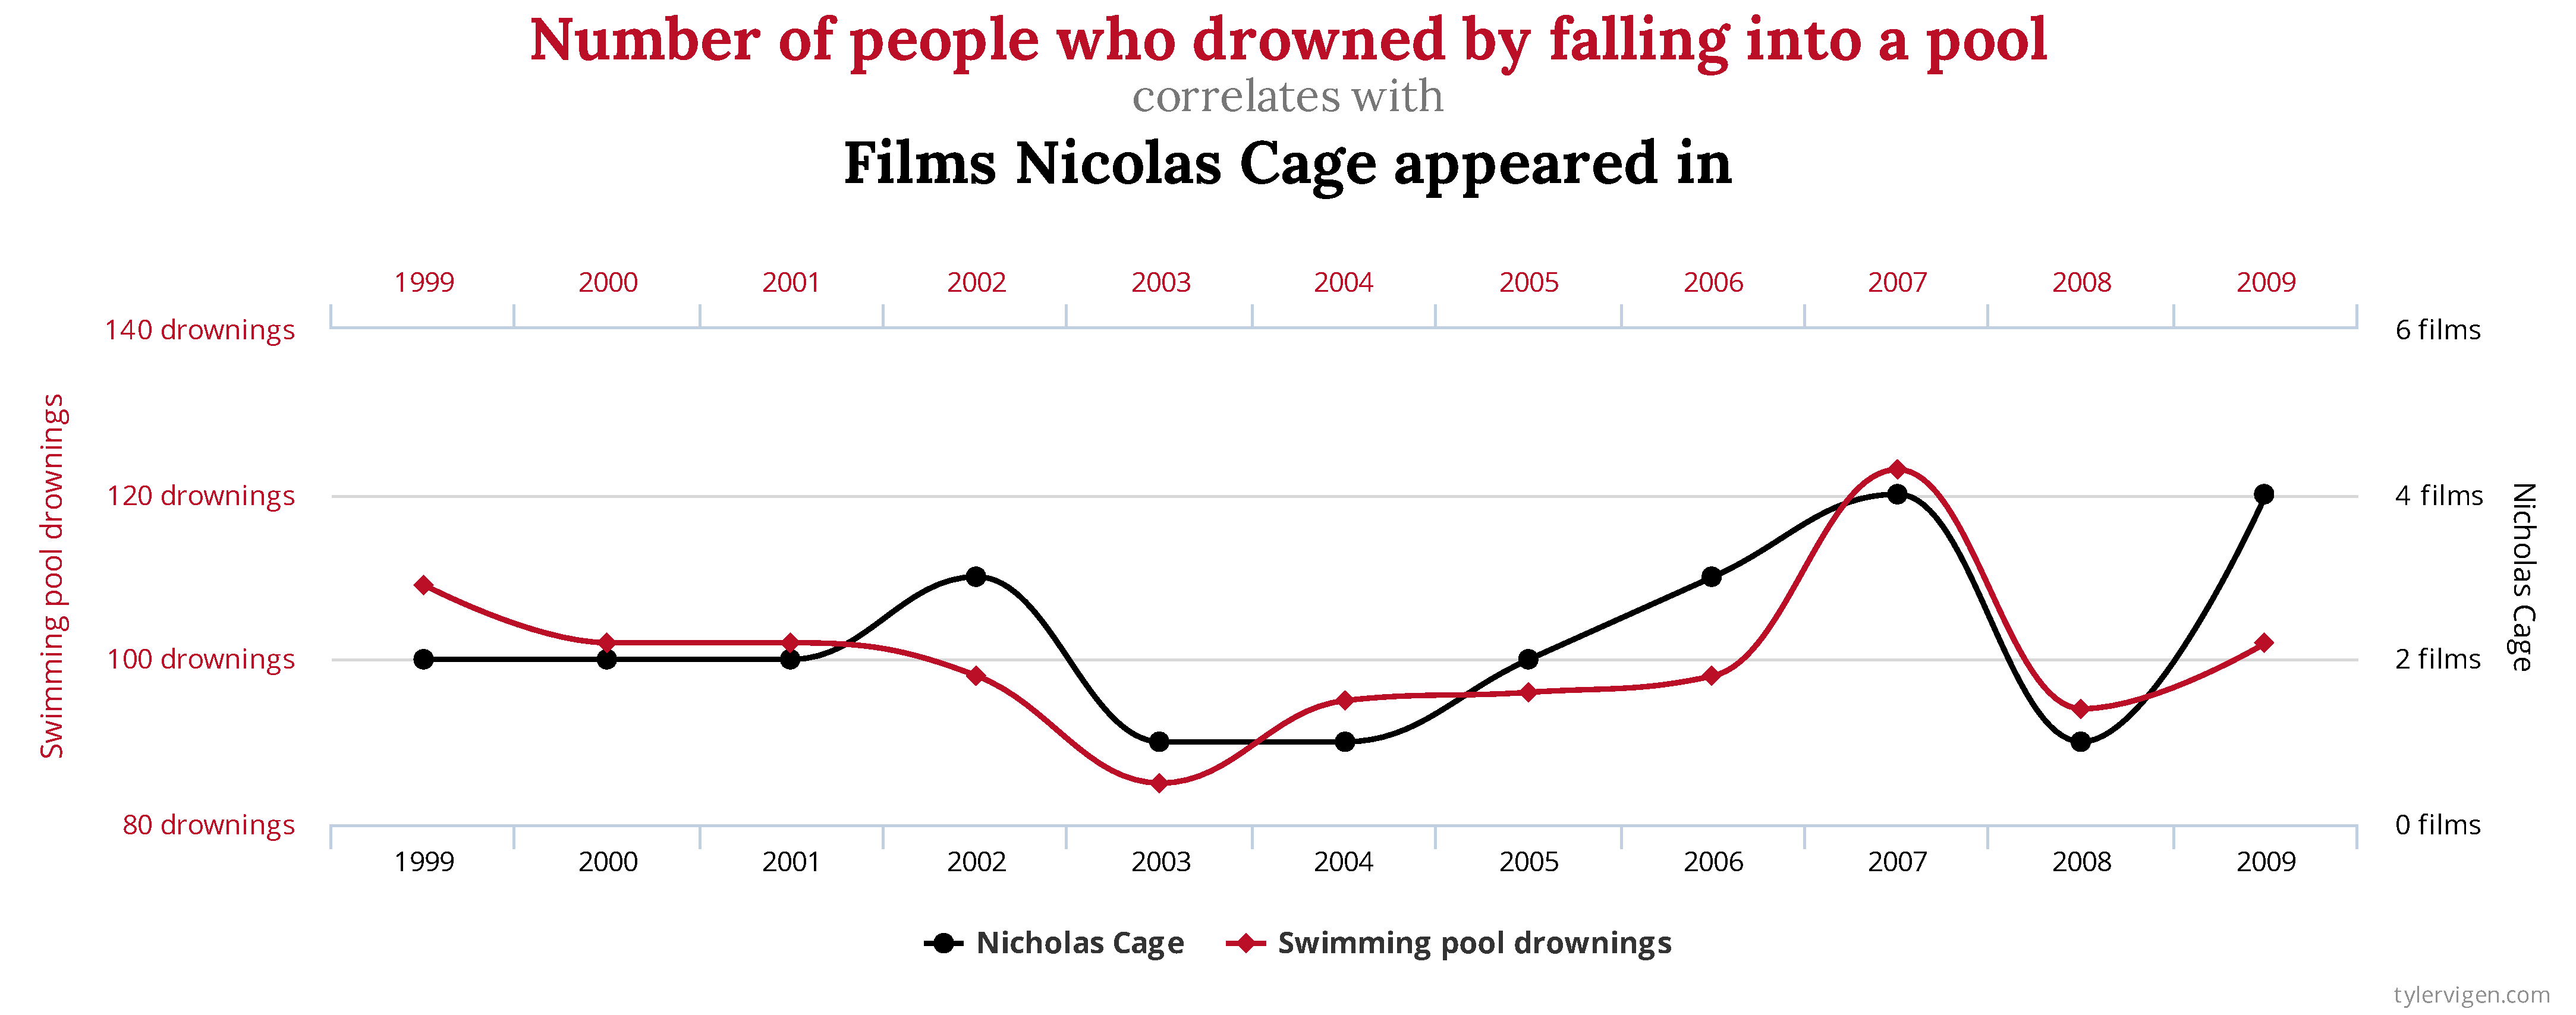
\includegraphics[scale=.23]{pooldiagram.pdf}
%%%%%%%%%%%%%%
%%%%%%%%%%%%%% image from pg 171
%%%%%%%%%%%%%%

These two phenomena vary directly, but it's hard to imagine how they could be causally related.
It's even more difficult to imagine how the following two phenomena could be causally related:

\noindent
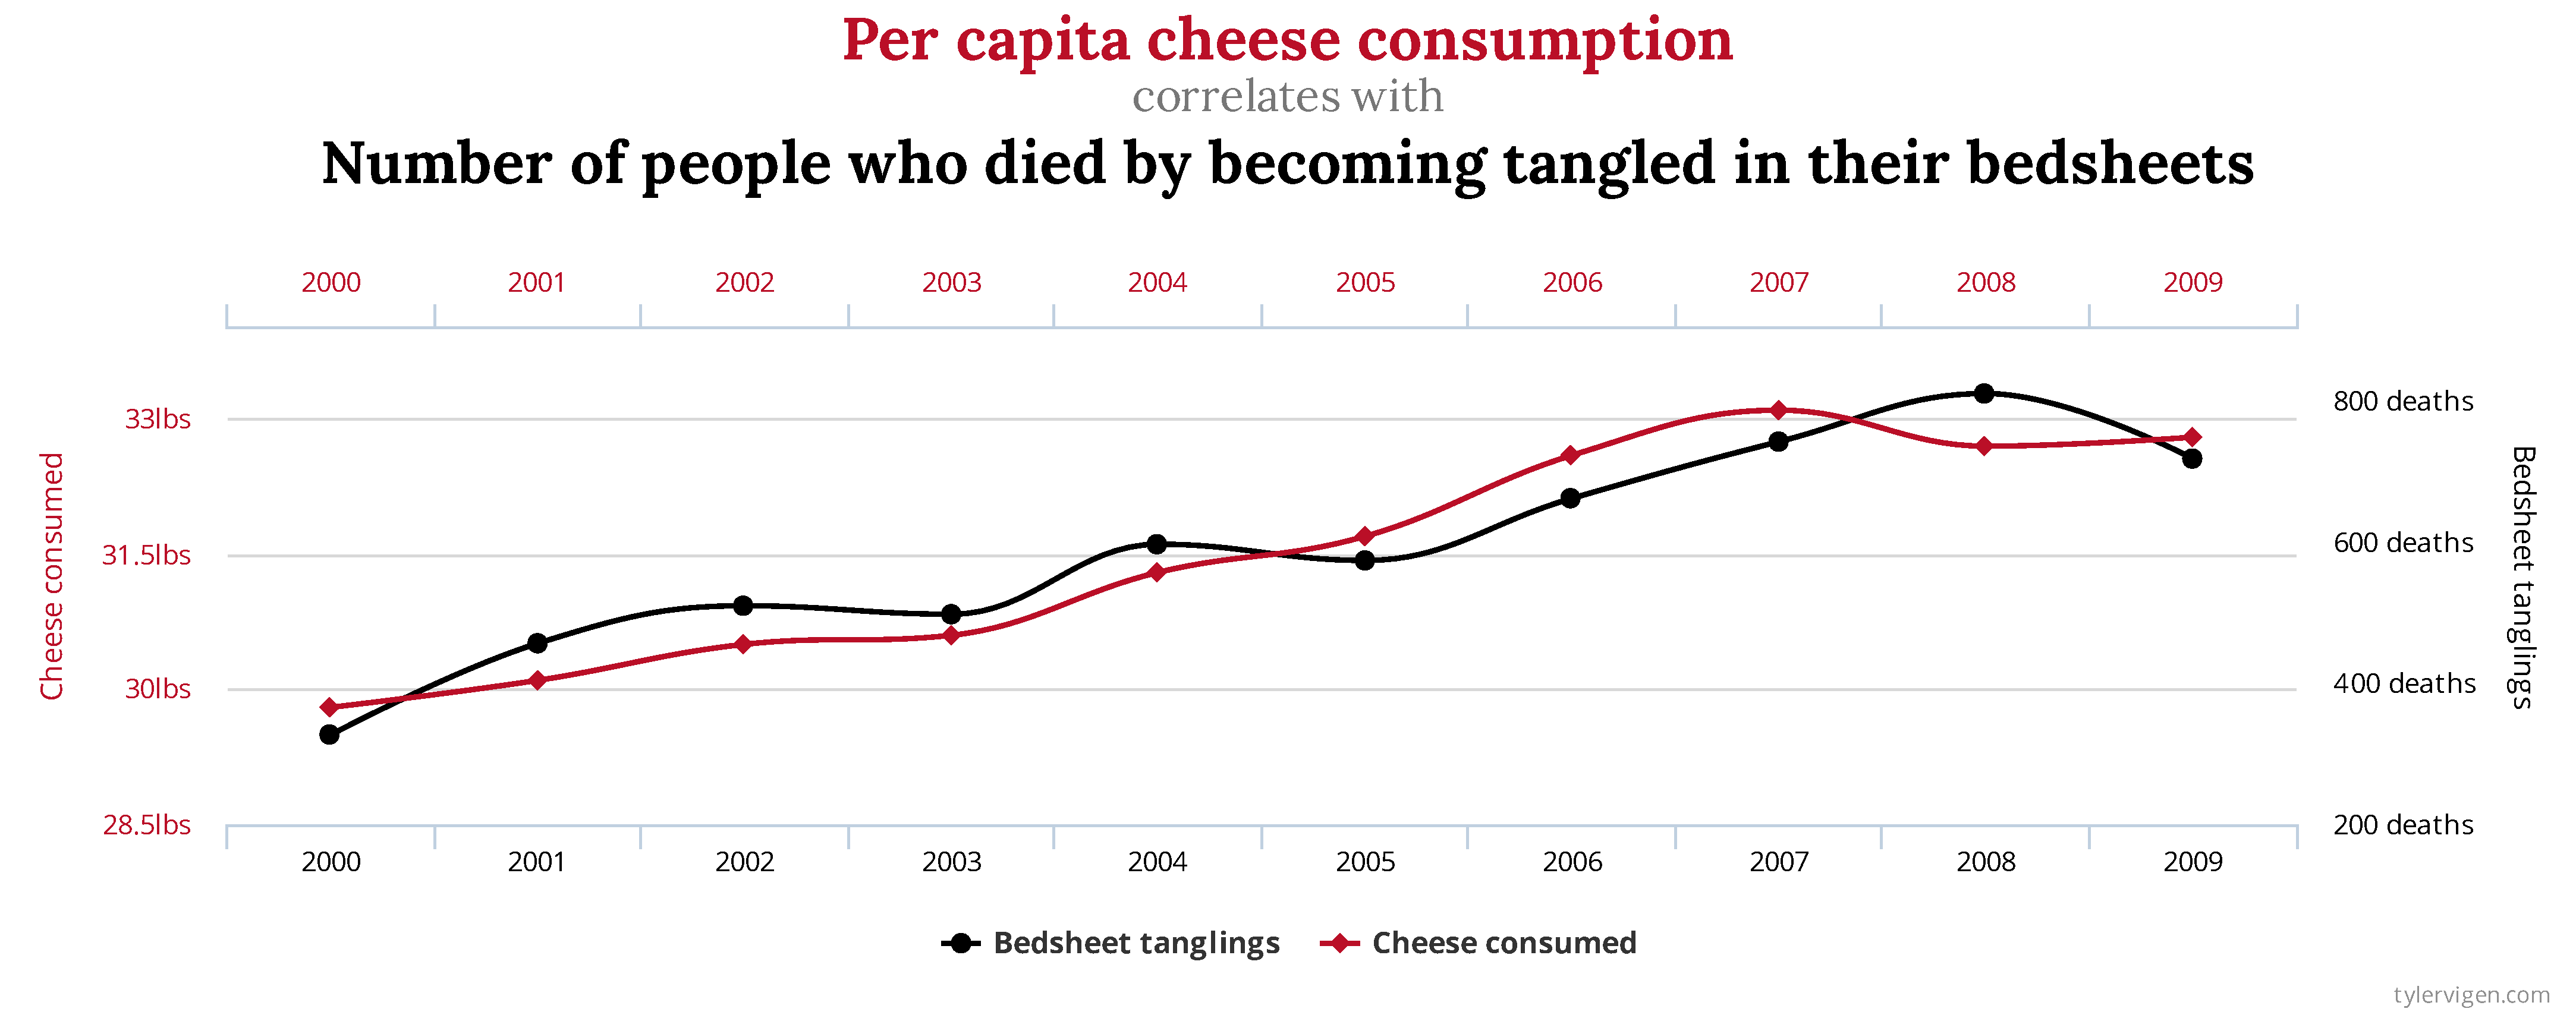
\includegraphics[scale=.23]{cheesediagram.pdf}
%%%%%%%%%%%%%%
%%%%%%%%%%%%%% image from pg 171
%%%%%%%%%%%%%%


So, Mill's Methods can't just be applied willy-nilly; one could end up ``discovering'' causal
connections where none exist. They can provide clues as to potential causal relationships, but care
and critical analysis are required to confirm those results. It's important to keep in mind that the
various methods can work in concert, providing a check on each other. If the drunken logician, for
example, had applied the Method of Difference--removing the 7-Up but keeping everything else
the same--he would have discovered his error (he would've kept getting hangovers). The
combination of the Methods of Agreement and Difference--the Joint Method, the controlled
study--is an invaluable tool in modern scientific research. A properly conducted controlled study
can provide quite convincing evidence of causal connections (or a lack thereof).

Of course, properly conducting a controlled study is not as easy as it sounds. It involves more than
just the application of the Joint Method of Agreement and Difference. There are other potentially
confounding factors that must be accounted for in order for such a study to yield reliable results.
For example, it's important to take great care in separating subjects into the test and control groups:
there can be no systematic difference between the two groups other than the factor that we're
testing; if there is, we cannot say whether the factor we're testing or the difference between the
groups is the cause of any effects observed. Suppose we were conducting a study to determine
whether or not vitamin C was effective in treating the common 
cold.\footnote{Despite widespread belief that it is, researchers have found very little evidence 
to support this claim.}
We gather 100 subjects
experiencing the onset of cold symptoms. We want one group of 50 to get vitamin C supplements,
and one group of 50--the control group--not to receive them. How do we decide who gets placed
into which group? We could ask for volunteers. But doing so might create a systematic difference
between the two groups. People who hear ``vitamin C'' and think, ``yeah, that's the group for me''
might be people who are more inclined to eat fruits and vegetables, for example, and might
therefore be healthier on average than people who are turned off by the idea of receiving vitamin
C supplements. This difference between the groups might lead to different results between the how
their colds progress. Instead of asking for volunteers, we might just assign the first 50 people who
show up to the vitamin C group, and the last 50 to the control group. But this could lead to
differences, as well. The people who show up earlier might be early-risers, who might be healthier
on average than those who straggle in late.

The best way to avoid systematic differences between test and control groups is to randomly assign
subjects to each. We refer to studies conducted this way as randomized controlled studies. And
besides randomization, other measures can be taken to improve reliability. The best kinds of
controlled studies are ``double-blind''. This means that neither the subjects nor the people
conducting the study know which group is the control and which group is receiving the actual
treatment. (This information is hidden from the researchers only while the study is ongoing; they
are told later, of course, so they can interpret the results.) This measure is necessary because of the
psychological tendency for people's observations to be biased based on their expectations. For
example, if the control group in our vitamin C experiment knew they were not getting any
treatment for their colds, they might be more inclined to report that they weren't feeling any better.
Conversely, if the members of the group receiving the vitamin supplements knew that they were
getting treated, they might be more inclined to report that their symptoms weren't as bad. This is
why the usual practice is to keep subjects in the dark about which group they're in, giving a placebo
to the members of the control group. It's important to keep the people conducting the study ``blind''
for the same reasons. If they knew which group was which, they might be more inclined to observe
improvement in the test group and a lack of improvement in the control group. In addition, in their
interactions with the subjects, they may unknowingly give away information about which group
was which via subconscious signals.

Hence, the gold standard for medical research (and other fields) is the double-blind controlled
study. It's not always possible to create those conditions--sometimes the best doctors can do is to
use the Method of Agreement and merely note commonalities amongst a group of patients
suffering from the same condition, for example--but the most reliable results come from such
tests. Discovering causes is hard in many contexts. Mill's Methods are a useful starting point, and
they accurately model the underlying inference patterns involved in such research, but in practice
they must be supplemented with additional measures and analytical rigor in order to yield
definitive results. They can give us clues about causes, but they aren't definitive evidence.
Remember, these are inductive, not deductive arguments. \\

EXERCISES \\

\begin{enumerate}
\item What is meant by the word `cause' in the following--necessary condition, sufficient condition,
or mere tendency?
\begin{enumerate}
\item (a) Throwing a brick through a window causes it to break.
\item (b) Slavery caused the American Civil War.
\item (c) Exposure to the cold causes frostbite.
\item (d) Running causes knee injuries.
\item (e) Closing your eyes causes you not to be able to see.
\end{enumerate}
\item Consider the following scenario and answer the questions about it:
\begin{itemize}
\item Alfonse, Bertram, Claire, Dominic, Ernesto, and Francine all go out to dinner at a local
greasy spoon. There are six items on the menu: shrimp cocktail, mushroom/barley soup,
burger, fries, steamed carrots, and ice cream. This is what they ate:
\end{itemize}
\begin{itemize}
\item Alfonse: shrimp, soup, fries
\item Bertram: burger, fries, carrots, ice cream
\item Claire: soup, burger, fries, carrots
\item Dominic: shrimp, soup, fries, ice cream
\item Ernesto: burger, fries, carrots
\item Francine: ice cream
\end{itemize}
\begin{itemize}
\item That night, Alfonse, Claire, and Dominic all came down with a wicked case of foodpoisoning. The others felt fine.
\end{itemize}
\begin{enumerate}
\item (a) Using only the Method of Agreement, how far can we narrow down the list of possible
causes for the food poisoning?
\item (b) Using only the Method of Difference, how far can we narrow down the list of possible
causes for the food poisoning?
\item (c) Using the Joint Method, we can identify the cause. What is it?
\end{enumerate}
\item For each of the following, identify which of Mill's Methods is being used to draw the causal
conclusion.
\begin{enumerate}
\item (a) A farmer noticed a marked increase in crop yields for the season. He started using a
new and improved fertilizer that year, and the weather was particularly ideal--just enough
rain and sunshine. Nevertheless, the increase was greater than could be explained by these
factors. So he looked into it and discovered that his fields had been colonized by
hedgehogs, who prey on the kinds of insect pests that usually eat crops.
\item (b) I've been looking for ways to improve the flavor of my vegan chili. I read on a website
that adding soy sauce can help: it has lots of umami flavor, and that can help compensate
for the lack of meat. So the other day, I made two batches of my chili, one using my usual
recipe, and the other made exactly the same way, except for the addition of soy sauce. I
invited a bunch of friends over for a blind taste test, and sure enough, the chili with the soy
sauce was the overwhelming favorite!
\item (c) The mere presence of guns in circulation can lead to higher murder rates. The data are
clear on this. In countries with higher numbers of guns per capita, the murder rate is higher;
and in countries with lower numbers of guns per capita, the murder rate is correspondingly
lower.
\item (d) There's a simple way to end mass shootings: outlaw semiautomatic weapons. In 1996,
Australia suffered the worst mass shooting episode in its history, when a man in Tasmania
used two semiautomatic rifles to kill 35 people (and wound an additional 19). The
Australian government responded by making such weapons illegal. There hasn't been a
mass shooting in Australia since.
\item (e) A pediatric oncologist was faced with a number of cases of childhood leukemia over a
short period of time. Puzzled, he conducted thorough examinations of all the children, and
also compared their living situations. He was surprised to discover that all of the children
lived in houses that were located very close to high-voltage power lines. He concluded that
exposure to electromagnetic fields causes cancer.
\item (f) Many people are touting the benefits of the so-called ``Mediterranean'' diet because it
apparently lowers the risk of heart disease. Residents of countries like Italy and Greece, for
example, consume large amounts of vegetables and olive oil and suffer from heart
problems at a much lower rate than Americans.
\item (g) My daughter came down with what appeared to be a run-of-the-mill case of the flu:
fever, chills, congestion, sore throat. But it was a little weird. She was also experiencing
really intense headaches and an extreme sensitivity to light. Those symptoms struck me as
atypical of mere influenza, so I took her to the doctor. It's a good thing I did! It turns out
she had a case of bacterial meningitis, which is so serious that it can cause brain damage if
not treated early. Luckily, we caught it in time and she's doing fine.
\end{enumerate}
\end{enumerate}
 

%1
%\chapter{Chapter 7}
Chapter6/ch6-2.tex %doing them the wrong way around on purpose
Chapter6/ch6-1.tex 

%1
%\chapter{Chapter 8}
Chapter7/ch7-1.tex
Chapter7/ch7-2.tex

%1
%\chapter{Chapter 9}
Chapter9/ch9-1.tex
\subsubsection{Slippery Slope}
Philosophers continue to argue and debate about how to resolve the sorites
paradox, but the point for us is just to illustrate the concept of vagueness. The
concept ``heap'' is a vague concept in this example. But so are so many other
concepts, such a color concepts (red, yellow, green, etc.), moral concepts (right,
wrong, good, bad), and just about any other concept you can think of. The one
domain that seems to be unaffected by vagueness is mathematical and logical
concepts. There are two fallacies related to vagueness: the causal slippery slope
and the conceptual slippery slope. We'll cover the conceptual slippery slope
first since it relates most closely to the concept of vagueness I've explained
above.

\paragraph{Conceptual slippery slope}
It may be true that there is no essential difference between 499 grains of sand
and 500 grains of sand. But even if that is so, it doesn't follow that there is no
difference between 1 grain of sand and 5 billion grains of sand. In general, just
because we cannot draw a distinction between A and B, and we cannot draw a
distinction between B and C, it doesn't mean we cannot draw a distinction
between A and C. Here is an example of a conceptual slippery slope fallacy.

\begin{quote}It is illegal for anyone under 21 to drink alcohol. But there is no
difference between someone who is 21 and someone who is 20 years 11
months old. So there is nothing wrong with someone who is 20 years and
11 months old drinking. But since there is no real distinction between
being one month older and one month younger, there shouldn't be
anything wrong with drinking at any age. Therefore, there is nothing
wrong with allowing a 10 year old to drink alcohol.\end{quote}

Imagine the life of an individual in stages of 1 month intervals. Even if it is true
that there is no distinction in kind between any one of those stages, it doesn't
follow that there isn't a distinction to be drawn at the extremes of either end.
Clearly there is a difference between a 5 year old and a 25 year old -- a
distinction in kind that is relevant to whether they should be allowed to drink
alcohol. The conceptual slippery slope fallacy assumes that because we cannot
draw a distinction between adjacent stages, we cannot draw a distinction at all
between any stages. One clear way of illustrating this is with color. Think of a
color spectrum from purple to red to orange to yellow to green to blue. Each
color grades into the next without there being any distinguishable boundaries
between the colors -- a continuous spectrum. Even if it is true that for any two
adjacent hues on the color wheel, we cannot distinguish between the two, it
doesn't follow from this that there is no distinction to be drawn between any two
portions of the color wheel, because then we'd be committed to saying that
there is no distinguishable difference between purple and yellow! The example
of the color spectrum illustrates the general point that just because the
boundaries between very similar things on a spectrum are vague, it doesn't
follow that there are no differences between any two things on that spectrum.
Whether or not one will identify an argument as committing a conceptual
slippery slope fallacy, depends on the other things one believes about the world.
Thus, whether or not a conceptual slippery slope fallacy has been committed will
often be a matter of some debate. It will itself be vague. Here is a good
example that illustrates this point.

People are found not guilty by reason of insanity when they cannot avoid
breaking the law. But people who are brought up in certain deprived
social circumstances are not much more able than the legally insane to
avoid breaking the law. So we should not find such individuals guilty any
more than those who are legally insane.

Whether there is conceptual slippery slope fallacy here depends on what you
think about a host of other things, including individual responsibility, free will,
the psychological and social effects of deprived social circumstances such as
poverty, lack of opportunity, abuse, etc. Some people may think that there are
big differences between those who are legally insane and those who grow up in
deprived social circumstances. Others may not think the differences are so
great. The issues here are subtle, sensitive, and complex, which is why it is
difficult to determine whether there is any fallacy here or not. If the differences
between those who are insane and those who are the product of deprived social
circumstances turn out to be like the differences between one shade of yellow
and an adjacent shade of yellow, then there is no fallacy here. But if the
differences turn out to be analogous to those between yellow and green (i.e.,
with many distinguishable stages of difference between) then there would
indeed be a conceptual slippery slope fallacy here.
The difficulty of
distinguishing instances of the conceptual slippery slope fallacy, and the fact
that distinguishing it requires us to draw on our knowledge about the world,
shows that the conceptual slippery slope fallacy is an informal fallacy.


\paragraph{Causal slippery slope fallacy}
The causal slippery slope fallacy is committed when one event is said to lead to
some other (usually disastrous) event via a chain of intermediary events. If you
have ever seen Direct TV's ``get rid of cable'' commercials, you will know exactly
what I'm talking about. (If you don't know what I'm talking about you should
Google it right now and find out. They're quite funny.) Here is an example of a
causal slippery slope fallacy (it is adapted from one of the Direct TV
commercials):

If you use cable, your cable will probably go on the fritz. If your cable is
on the fritz, you will probably get frustrated. When you get frustrated you
will probably hit the table. When you hit the table, your young daughter
will probably imitate you. When your daughter imitates you, she will
probably get thrown out of school. When she gets thrown out of school,
she will probably meet undesirables. When she meets undesirables, she
will probably marry undesirables. When she marries undesirables, you
will probably have a grandson with a dog collar. Therefore, if you use
cable, you will probably have a grandson with dog collar.

This example is silly and absurd, yes. But it illustrates the causal slippery slope
fallacy. Slippery slope fallacies are always made up of a series of conjunctions of
probabilistic conditional statements that link the first event to the last event. A
causal slippery slope fallacy is committed when one assumes that just because
each individual conditional statement is probable, the conditional that links the
first event to the last event is also probable. Even if we grant that each ``link'' in
the chain is individually probable, it doesn't follow that the whole chain (or the
conditional that links the first event to the last event) is probable. Suppose, for
the sake of the argument, we assign probabilities to each ``link'' or conditional
statement, like this. (I have italicized the consequents of the conditionals and
assigned high conditional probabilities to them. The high probability is for the
sake of the argument; I don't actually think these things are as probable as I've
assumed here.)

\begin{quote}
If you use cable, then your cable will probably go on the fritz (.9) \\
If your cable is on the fritz, then you will probably get angry (.9) \\
If you get angry, then you will probably hit the table (.9) \\
If you hit the table, your daughter will probably imitate you (.8) \\
If your daughter imitates you, she will probably be kicked out of school (.8) \\
If she is kicked out of school, she will probably meet undesirables (.9) \\
If she meets undesirables, she will probably marry undesirables (.8) \\
If she marries undesirables, you will probably have a grandson with a dog collar (.8) \\
\end{quote}

However, even if we grant the probabilities of each link in the chain is high (80-90\% 
probable), the conclusion doesn't even reach a probability higher than
chance. Recall that in order to figure the probability of a conjunction, we must
multiply the probability of each conjunct:

\begin{quote}(.9) x (.9) x (.9) x (.8) x (.8) x (.9) x (.8) x (.8) = .27
\end{quote}

That means the probability of the conclusion (i.e., that if you use cable, you will
have a grandson with a dog collar) is only 27\%, 
despite the fact that each
conditional has a relatively high probability! The causal slippery slope fallacy is
actually a formal probabilistic fallacy and so could have been discussed in
chapter 3 with the other formal probabilistic fallacies. What makes it a formal
rather than informal fallacy is that we can identify it without even having to know
what the sentences of the argument mean. I could just have easily written out a
nonsense argument comprised of series of probabilistic conditional statements.
But I would still have been able to identify the causal slippery slope fallacy
because I would have seen that there was a series of probabilistic conditional
statements leading to a claim that the conclusion of the series was also probable.
That is enough to tell me that there is a causal slippery slope fallacy, even if I
don't really understand the meanings of the conditional statements.

It is helpful to contrast the causal slippery slope fallacy with the valid form of
inference, hypothetical syllogism. Recall that a hypothetical syllogism has the
following kind of form:

\begin{quote}
A$\rightarrow$ B \\
B$\rightarrow$ C \\
C$\rightarrow$ D \\
D$\rightarrow$ E \\
So, A$\rightarrow$ E \\
\end{quote}

The only difference between this and the causal slippery slope fallacy is that
whereas in the hypothetical syllogism, the link between each component is
certain, in a causal slippery slope fallacy, the link between each event is
probabilistic. It is the fact that each link is probabilistic that accounts for the
fallacy. One way of putting this is point is that probability is not transitive. Just
because A makes B probable and B makes C probable and C makes X probable,
it doesn't follow that A makes X probable. In contrast, when the links are certain
rather than probable, then if A always leads to B and B always leads to C and C
always leads to X, then it has to be the case that A always leads to X.



%1
%\chapter{Chapter 10}
%this chapter takes sections from "fundamentals" and also "introduction", Chapter 4, 186-194
\chapter{Fallacies of Illicit Presumption}
This is a family of fallacies whose common characteristic is that they (often tacitly, implicitly)
presume the truth of some claim that they're not entitled to. They are arguments with a premise
(again, often hidden) that is assumed to be true, but is actually a controversial claim, which at best
requires support that's not provided, which at worst is simply false. We will look at six fallacies
under this heading.

\subsubsection{Accident}
This fallacy is the reverse of the hasty generalization. That was a fallacious inference from
insufficient particular premises to a general conclusion; accident is a fallacious inference from a
general premise to a particular conclusion. What makes it fallacious is an illicit presumption: the
general rule in the premise is assumed, incorrectly, not to have any exceptions; the particular
conclusion fallaciously inferred is one of the exceptional cases.

Here's a simple example to help make that clear:

\begin{quote}Cutting people with knives is illegal. \\
\underline{Surgeons cut people with knives.} \\
Surgeons should be arrested. \end{quote}

One of the premises is the general claim that cutting people with knives is illegal. While this is
true in almost all cases, there are exceptions--surgery among them. We pay surgeons lots of
money to cut people with knives! It is therefore fallacious to conclude that surgeons should be
arrested, since they are an exception to the general rule. The inference only goes through if we
presume, incorrectly, that the rule is exceptionless.

Another example. Suppose I volunteer at my first grade daughter's school; I go in to her class one
day to read a book aloud to the children. As I'm sitting down on the floor with the kiddies, 
crisscross applesauce, as they say, I realize that I can't comfortably sit that way because of the .44
Magnum revolver that I have tucked into my waistband.\footnote{That's Dirty Harry's gun, ``the most powerful handgun in the world."} 
So I remove the piece from my pants
and set it down on the floor in front of me, among the circled-up children. The teacher screams
and calls the office, the police are summoned, and I'm arrested. As they're hauling me out of the
room, I protest: ``The Second Amendment to the Constitution guarantees my right to keep and bear
arms! This state has a `concealed carry' law, and I have a license to carry that gun! Let me go!"

I'm committing the fallacy of Accident in this story. True, the Second Amendment guarantees the
right to keep and bear arms; but that rule is not without exceptions. Similarly, concealed carry laws
also have exceptions--among them being a prohibition on carrying weapons into elementary
schools. My insistence on being released only makes sense if we presume, incorrectly, that the
legal rules I'm citing are without exception.

One more example from real life. After the financial crisis in 2008, the Federal Reserve--the
central bank in the United States, whose task it is to create conditions leading to full employment
and moderate inflation--found itself in a bind. The economy was in a free-fall, and unemployment
rates were skyrocketing, but the usual tool it used to mitigate such problems--cutting the shortterm federal funds rate (an interest rate banks charge each other for overnight loans)--was
unavailable, because they had already cut the rate to zero (the lowest it could go). So they had to
resort to unconventional monetary policies, among them something called ``quantitative easing".
This involved the purchase, by the Federal Reserve, of financial assets like mortgage-backed
securities and longer-term government debt 
(Treasury notes).\footnote{The hope was to push down interest rates on mortgages and government debt, encouraging people to buy houses
and spend money instead of saving it--thus stimulating the economy.}

Now, the nice thing about being the Federal Reserve is that when you want to buy something--in
this case a bunch of financial assets--it's really easy to pay for it: you have the power to create
new money out of thin air! That's what the Federal Reserve does; it controls the amount of money
that exists. So if the Fed wants to buy, say, \$10 million worth of securities from Bank of America,
they just press a button and presto--\$10 million dollars that didn't exist a second ago comes into
being as an asset of Bank of 
America.\footnote{It's obviously a bit more complicated than that, but that's the essence of it.}

This quantitative easing policy was controversial. Many people worried that it would lead to
runaway inflation. Generally speaking, the more money there is, the less each bit of it is worth. So
creating more money makes things cost more--inflation. The Fed was creating money on a very
large scale--on the order of a trillion dollars. Shouldn't that lead to a huge amount of inflation?

Economist Art Laffer thought so. In June of 2009, he wrote an op-ed in the Wall Street Journal
warning that ``[t]he unprecedented expansion of the money supply could make the '70s look
benign."\footnote{Art Laffer, ``Get Ready for Inflation and Higher Interest Rates," June 11, 2009, Wall Street Journal}
(There was a lot of inflation in the '70s.)

Another famous economist, Paul Krugman, accused Laffer of committing the fallacy of accident.
While it's generally true that an increase in the supply of money leads to inflation, that rule is not
without exceptions. He had described such exceptional circumstances in 
1998\footnote{``But if current prices are not downwardly flexible, and the public expects price stability in the long run, the economy
cannot get the expected inflation it needs; and in that situation the economy finds itself in a slump against which shortrun monetary expansion, no matter how large, is ineffective." From Paul Krugman, "It's baack: Japan's Slump and the
Return of the Liquidity Trap," 1998, Brookings Papers on Economic Activity, 2}, 
and pointed out
that the economy of 2009 was in that condition (which economists call a ``liquidity trap"): ``Let me
add, for the 1.6 trillionth time, we are in a liquidity trap. And in such circumstances a rise in the
monetary base does not lead to 
inflation."\footnote{Paul Krugman, June 13, 2009, The New York Times}

It turns out Krugman was correct. The expansion of the monetary supply did not lead to runaway
inflation; as a matter of fact, inflation remained below the level that the Federal Reserve wanted,
barely moving at all. Laffer had indeed committed the fallacy of accident.

\subsubsection{Begging the Question (Petitio Principii)}
First things first: `begging the question' is not synonymous with `raising the question'; this is an
extremely common usage, but it is wrong. You might hear a newscaster say, ``Today Donald
Trump's private jet was spotted at the Indianapolis airport, which begs the question: `Will he
choose Indiana Governor Mike Pence as running mate?'" This is a mistaken usage of `begs the
question'; the newscaster should have said `raises the question' instead.

'Begging the question' is a translation of the Latin `petitio principii', which refers to the practice
of asking (begging, petitioning) your audience to grant you the truth of a claim (principle) as a
premise in an argument--but it turns out that the claim you're asking for is either identical to, or
presupposes the truth of, the very conclusion of the argument you're trying to make.

In other words, when you beg the question, you're arguing in a circle: one of the reasons for
believing the conclusion is the conclusion itself! It's a Fallacy of Illicit Presumption where the
proposition being presumed is the very proposition you're trying to demonstrate; that's clearly an
illicit presumption.

Here's a stark example. If I'm trying to convince you that Donald Trump is a dangerous idiot (the
conclusion of my argument is `Donald Trump is a dangerous idiot'), then I can't ask you to grant
me the claim `Donald Trump is a dangerous idiot'. The premise can't be the same as the conclusion.
Imagine a conversation:

\begin{quote}
Me: ``Donald Trump is a dangerous idiot." \\
You: ``Really? Why do you say that?" \\
Me: ``Because Donald Trump is a dangerous idiot." \\
You: ``So you said. But why should I agree with you? Give me some reasons." \\
Me: ``Here's a reason: Donald Trump is a dangerous idiot."
\end{quote}

And round and round we go. Circular reasoning; begging the question.

It's not always so blatant. Sometimes the premise is not identical to the conclusion, but merely
presupposes its truth. Why should we believe that the Bible is true? Because it says so right there
in the Bible that it's the infallible Word of God. This premise is not the same as the conclusion,
but it can only support the conclusion if we take the Bible's word for its own truthfulness, i.e., if
we assume that the Bible is true. But that was the very claim we were trying to prove!

Sometimes the premise is just a re-wording of the conclusion. Consider this argument: ``To allow
every man unbounded freedom of speech must always be, on the whole, advantageous to the state;
for it is highly conducive to the interests of the community that each individual should enjoy a
liberty, perfectly unlimited, of expressing his 
sentiments."\footnote{This is a classic example, from Richard Whately's 1826 Elements of Logic.}
Replacing synonyms with synonyms,
this comes down to ``Free speech is good for society because free speech is good for society." Not
a good argument.\footnote{Though it's valid! P, therefore P is a valid form: if the premise is true, the conclusion must be; they're the same.}

%%%%%%here's the bit from "intro" pg 189
Consider the following argument:

\begin{quote}      Capital punishment is justified for crimes such as rape and murder
      because it is quite legitimate and appropriate for the state to put to
      death someone who has committed such heinous and inhuman acts.\end{quote}

The premise indicator, ``because" denotes the premise and (derivatively) the
conclusion of this argument. In standard form, the argument is this:

\begin{quote}\underline{It is legitimate and appropriate for the state to put to death someone
          who commits rape or murder.}\\
      2. Therefore, capital punishment is justified for crimes such as rape and
          murder.\end{quote}

You should notice something peculiar about this argument: the premise is
essentially the same claim as the conclusion. The only difference is that the
premise spells out what capital punishment means (the state putting criminals to
death) whereas the conclusion just refers to capital punishment by name, and
the premise uses terms like ``legitimate" and ``appropriate" whereas the
conclusion uses the related term, ``justified." But these differences don't add up
to any real differences in meaning. Thus, the premise is essentially saying the
same thing as the conclusion. This is a problem: we want our premise to
provide a reason for accepting the conclusion. But if the premise is the same
claim as the conclusion, then it can't possibly provide a reason for accepting the
conclusion! Begging the question occurs when one (either explicitly or
implicitly) assumes the truth of the conclusion in one or more of the premises.
Begging the question is thus a kind of circular reasoning.

One interesting feature of this fallacy is that formally there is nothing wrong with
arguments of this form. Here is what I mean. Consider an argument that
explicitly commits the fallacy of begging the question. For example,

        \begin{quote}\underline{Capital punishment is morally permissible} \\
       Therefore, capital punishment is morally permissible \end{quote}

Now, apply any method of assessing validity to this argument and you will see
that it is valid by any method. If we use the informal test (by trying to imagine
that the premises are true while the conclusion is false), then the argument
passes the test, since any time the premise is true, the conclusion will have to be
true as well (since it is the exact same statement). Likewise, the argument is
valid by our formal test of validity, truth tables. But while this argument is
technically valid, it is still a really bad argument. Why? Because the point of
giving an argument in the first place is to provide some reason for thinking the
conclusion is true for those who don't already accept the conclusion. But if one
doesn't already accept the conclusion, then simply restating the conclusion in a
different way isn't going to convince them. Rather, a good argument will
provide some reason for accepting the conclusion that is sufficiently
independent of that conclusion itself. Begging the question utterly fails to do
this and this is why it counts as an informal fallacy. What is interesting about
begging the question is that there is absolutely nothing wrong with the
argument formally.

Whether or not an argument begs the question is not always an easy matter to
sort out.      As with all informal fallacies, detecting it requires a careful
understanding of the meaning of the statements involved in the argument. Here
is an example of an argument where it is not as clear whether there is a fallacy of
begging the question:

\begin{quote}        Christian belief is warranted because according to Christianity there exists
        a being called ``the Holy Spirit" which reliably guides Christians towards
        the truth regarding the central claims of Christianity.\footnote{This is a much simplified version of the view defended by Christian philosophers such as Alvin
Plantinga. Plantinga defends (something like) this claim in: Plantinga, A. 2000. Warranted
Christian Belief. Oxford, UK: Oxford University Press.}
\end{quote}

One might think that there is a kind of circularity (or begging the question)
involved in this argument since the argument appears to assume the truth of
Christianity in justifying the claim that Christianity is true. But whether or not this
argument really does beg the question is something on which there is much
debate within the sub-field of philosophy called epistemology (``study of
knowledge"). The philosopher Alvin Plantinga argues persuasively that the
argument does not beg the question, but being able to assess that argument
takes patient years of study in the field of epistemology (not to mention a careful
engagement with Plantinga's work). As this example illustrates, the issue of
whether an argument begs the question requires us to draw on our general
knowledge of the world. This is the mark of an informal, rather than formal,
fallacy.
 %%%%%%%%%%end stuff from "intro" pg 191


\subsubsection{Loaded Questions}
Loaded questions are questions the very asking of which presumes the truth of some claim. Asking
these can be an effective debating technique, a way of sneaking a controversial claim into the
discussion without having outright asserted it.

The classic example of a loaded question is, ``Have you stopped beating your wife?" Notice that
this is a yes-or-no question, and no matter which answer one gives, one admits to beating his wife:
if the answer is `no', then the person continues to beat his wife; if the answer is `yes', then he
admits to beating his wife in the past. Either way, he's a wife-beater. The question itself presumes
the truth of this claim; that's what makes it ``loaded".

Strategic deployment of loaded yes-or-no questions can be an extremely effective debating
technique. If you catch your opponent off-guard, they will struggle to respond to your question,
since a simple `yes' or `no' commits them to the truth of the illicit presumption, which they want
to deny. This makes them look evasive, shifty. And as they struggle to come up with a response,
you can pounce on them: ``It's a simple question. Yes or no? Why won't you answer the question?"
It's a great way to appear to be winning a debate, even if you don't have a good argument. Imagine
the following dialogue:

\begin{quote}
Liberal TV Host: ``Are you or are you not in favor of the president's plan to force wealthy
business owners to pay their fair share in taxes to protect the vulnerable and aid this nation's
underprivileged?" \\
Conservative Guest: ``Well, I don't agree with the way you've laid out the question. As a
matter of fact\dots" \\
Host: ``It's a simple question. Should business owners pay their fair share; yes or no?" \\
Guest: ``You're implying that the president's plan would correct some injustice. But
corporate taxes are already very \dots" \\
Host: ``Stop avoiding the question! It's a simple yes or no!" \\
\end{quote}

Combine this with the sort of subconscious appeal to force discussed above--yelling, fingerpointing, etc.--and 
the host might come off looking like the winner of the debate, with his
opponent appearing evasive, uncooperative, and inarticulate.

Another use for loaded questions is the particularly sneaky political practice of ``push polling". In
a normal opinion poll, you call people up to try to discover what their views are about the issues.
In a push poll, you call people up pretending to be conducting a normal opinion poll, pretending
only to be interested in discovering their views, but with a different intention entirely: you don't
want to know what their views are; you want to shape their views, to convince them of something.
And you use loaded questions to do it.

A famous example of this occurred during the Republican presidential primary in 2000. George
W. Bush was the front-runner, but was facing a surprisingly strong challenge from the upstart John
McCain. After McCain won the New Hampshire primary, he had a lot of momentum. The next
state to vote was South Carolina; it was very important for the Bush campaign to defeat McCain
there and reclaim the momentum. So they conducted a push poll designed to spread negative
feelings about McCain--by implanting false beliefs among the voting public. ``Pollsters" called
voters and asked, ``Would you be more or less likely to vote for John McCain for president if you
knew he had fathered an illegitimate black child?" The aim, of course, is for voters to come to
believe that McCain fathered an illegitimate black child. But he did no such thing. He and his
wife adopted a daughter, Bridget, from Bangladesh.

A final note on loaded questions: there's a minimal sense in which every question is loaded. The
social practice of asking questions is governed by implicit norms. One of these is that it's only
appropriate to ask a question when there's some doubt about the answer. So every question carries
with it the presumption that this norm is being adhered to, that it's a reasonable question to ask,
that the answer is not certain. One can exploit this fact, again to plant beliefs in listeners' minds
that they otherwise wouldn't hold. In a particularly shameful bit of alarmist journalism, the cover
of the July 1, 2016 issue of Newsweek asks the question, ``Can ISIS Take Down Washington?" The
cover is an alarming, eye-catching shade of yellow, and shows four missiles converging on the
Capitol dome. The simple answer to the question, though, is `no, of course not'. There is no
evidence that ISIS has the capacity to destroy the nation's capital. But the very asking of the
question presumes that it's a reasonable thing to wonder about, that there might be a reason to
think that the answer is `yes'. The goal is to scare readers (and sell magazines) by getting them to
believe there might be such a threat.

\subsubsection{False Choice}
This fallacy occurs when someone tries to convince you of something by presenting it as one of
limited number of options and the best choice among those options. The illicit presumption is that
the options are limited in the way presented; in fact, there are additional options that are not
offered. The choice you're asked to make is a false choice, since not all the possibilities have been
presented.

Most frequently, the number of options offered is two. In this case, you're being presented with a
false dilemma. I manipulate my kids with false choices all the time. My younger daughter, for
example, loves cucumbers; they're her favorite vegetable by far. We have a rule at dinner: you've
got to choose a vegetable to eat. Given her 'druthers, she'd choose cucumber every night. Carrots
are pretty good, too; they're the second choice. But I need her to have some more variety, so I'll
sometimes lie and tell her we're out of cucumbers and carrots, and that we only have two options:
broccoli or green beans, for example. That's a false choice; I've deliberately left out other options.
I give her the false choice as a way of manipulating her into choosing green beans, because I know
she dislikes broccoli.

Politicians often treat us like children, presenting their preferred policies as the only acceptable
choice among an artificially restricted set of options. We might be told, for example, that we need
to raise the retirement age or cut Social Security benefits across the board; the budget can't keep
up with the rising number of retirees. Well, nobody wants to cut benefits, so we have to raise the
retirement age. Bummer. But it's a false choice. There are any number of alternative options for
funding an increasing number of retirees: tax increases, re-allocation of other funds, means-testing
for benefits, etc.

Liberals are often ambivalent about free trade agreements. On the one hand, access to American
markets can help raise the living standards of people from poor countries around the world; on the
other hand, such agreements can lead to fewer jobs for American workers in certain sectors of the
economy (e.g., manufacturing). So what to do? Support such agreements or not? Seems like an
impossible choice: harm the global poor or harm American workers. But it may be a false choice,
as this economist argues:

\begin{quote}But trade rules that are more sensitive to social and equity concerns in the advanced
countries are not inherently in conflict with economic growth in poor countries.
Globalization's cheerleaders do considerable damage to their cause by framing the issue as
a stark choice between existing trade arrangements and the persistence of global poverty.
And progressives needlessly force themselves into an undesirable tradeoff.
… Progressives should not buy into a false and counter-productive narrative that sets the
interests of the global poor against the interests of rich countries' lower and middle classes.
With sufficient institutional imagination, the global trade regime can be reformed to the
benefit of both.\footnote{Dani Rodrik, ``A Progressive Logic of Trade," Project Syndicate, 4/13/2016}
\end{quote}

When you think about it, almost every election in America is a False Choice. With the dominance of the two major political parties, we're normally presented with a stark, sometimes 
unpalatable, choice between only two options: the Democrat or the Republican. But of course if enough people decided to vote for a third-party candidate, that person could win. Such 
candidates do exist. But it's perceived as wasting a vote when you choose someone like that. This fact was memorably highlighted on The Simpsons back in the fall of 1996, before the 
presidential election between Bill Clinton and Bob Dole. In the episode, the diabolical, scheming aliens Kang and Kodos (the green guys with the tentacles and giant heads who drool 
constantly) contrive to abduct the two majorparty candidates and perform a ``bio-duplication" procedure that allows Kang and Kodos to appear as Dole and Clinton, respectively. The 
disguised aliens hit the campaign trail and give speeches, making bizarre campaign 
promises.\footnote{Kodos: ``I am Clin-ton. As overlord, all will kneel trembling before me and obey my brutal command. End
communication."} 
When Homer reveals the subterfuge to a horrified crowd, Kodos taunts the voters: ``It's 
true; we are aliens. But what are you going to do about it? It's a twoparty system. You have to vote for one of us." When a guy in the crowd declares his intention to vote for a 
third-party candidate, Kang responds, ``Go ahead, throw your vote away!" Then Kang and Kodos laugh maniacally. Later, as Marge and Homer--chained together and wearing neckcollars--are 
being whipped by an alien slave-driver, Marge complains and Homer quips, ``Don't blame me; I voted for Kodos."

\subsubsection{Composition}
The fallacy of Composition rests on an illicit presumption about the relationship between a whole
thing and the parts that make it up. This is an intuitive distinction, between whole and parts: for
example, a person can be considered as a whole individual thing; it is made up of lots of parts--
hands, feet, brain, lungs, etc., etc. We commit the fallacy of Composition when we mistakenly
assume that any property that all of the parts share is also a property of the whole. Schematically,
it looks like this:

\begin{quote}
All of the parts of X have property P. \\
\underline{Any property shared by all of the parts of a thing is also a property of the whole.} \\
X has the property P.\end{quote}

The second premise is the illicit presumption that makes this argument go through. It is illicit
because it is simply false: sometimes all the parts of something have a property in common, but
the whole does not have that property.

Consider the 1980 U.S. Men's Hockey Team. They won the gold medal at the Olympics that year,
beating the unstoppable-seeming Russian team in the semifinals. (That game is often referred to
as ``The Miracle on Ice" after announcer Al Michaels' memorable call as the seconds ticked off at
the end: ``Do you believe in miracles? Yes!") Famously, the U.S. team that year was a rag-tag
collection of no-name college guys; the average age on the team was 21, making them the youngest
team ever to compete for the U.S. in the Olympics. The Russian team, on the other hand, was
packed with seasoned hockey veterans with world-class talent.

In this example, the team is the whole, and the individual players on the team are the parts. It's
safe to say that one of the properties that all of the parts shared was mediocrity--at least, by the
standards of international competition at the time. They were all good hockey players, of course--
Division I college athletes--but compared to the Hall of Famers the Russians had, they were
mediocre at best. So, all of the parts have the property of being mediocre. But it would be a mistake
to conclude that the whole made up of those parts--the 1980 U.S. Men's Hockey Team--also had
that property. The team was not mediocre; they defeated the Russians and won the gold medal!
They were a classic example of the whole being greater than the sum of its parts.

%%%%%%%%begin "intro" pg 186
Consider the following argument:

\begin{quote}      Each member on the gymnastics team weighs less than 110 lbs.
      Therefore, the whole gymnastics team weighs less than 110 lbs.\end{quote}

This arguments commits the composition fallacy. In the composition fallacy one
argues that since each part of the whole has a certain feature, it follows that the
whole has that same feature. However, you cannot generally identify any
argument that moves from statements about parts to statements about wholes
as committing the composition fallacy because whether or not there is a fallacy
depends on what feature we are attributing to the parts and wholes. Here is an
example of an argument that moves from claims about the parts possessing a
feature to a claim about the whole possessing that same feature, but doesn't
commit the composition fallacy:

\begin{quote}        Every part of the car is made of plastic. Therefore, the whole car is made
        of plastic. \end{quote}

This conclusion does follow from the premises; there is no fallacy here. The
difference between this argument and the preceding argument (about the
gymnastics team) isn't their form. In fact both arguments have the same form:
       
\begin{quote} Every part of X has the feature f. Therefore, the whole X has the feature f.\end{quote}

And yet one of the arguments is clearly fallacious, while the other isn't. The
difference between the two arguments is not their form, but their content. That
is, the difference is what feature is being attributed to the parts and wholes.
Some features (like weighing a certain amount) are such that if they belong to
each part, then it does not follow that they belong to the whole. Other features
(such as being made of plastic) are such that if they belong to each part, it
follows that they belong to the whole.

Here is another example:

\begin{quote}        Every member of the team has been to Paris. Therefore the team has
        been to Paris.\end{quote}

The conclusion of this argument does not follow. Just because each member of
the team has been to Paris, it doesn't follow that the whole team has been to
Paris, since it may not have been the case that each individual was there at the
same time and was there in their capacity as a member of the team. Thus, even
though it is plausible to say that the team is composed of every member of the
team, it doesn't follow that since every member of the team has been to Paris,
the whole team has been to Paris. Contrast that example with this one:

\begin{quote}       Every member of the team was on the plane. Therefore, the whole team
       was on the plane.\end{quote}

This argument, in contrast to the last one, contains no fallacy. It is true that if
every member is on the plane then the whole team is on the plane. And yet
these two arguments have almost exactly the same form. The only difference is
that the first argument is talking about the property, having been to Paris,
whereas the second argument is talking about the property, being on the plane.
The only reason we are able to identify the first argument as committing the
composition fallacy and the second argument as not committing a fallacy is that
we understand the relationship between the concepts involved. In the first case,
we understand that it is possible that every member could have been to Paris
without the team ever having been; in the second case we understand that as
long as every member of the team is on the plane, it has to be true that the
whole team is on the plane. The take home point here is that in order to identify
whether an argument has committed the composition fallacy, one must
understand the concepts involved in the argument. This is the mark of an
informal fallacy: we have to rely on our understanding of the meanings of the
words or concepts involved, rather than simply being able to identify the fallacy
from its form.
%%%%%%%%end "intro" page 188

\subsubsection{Division}
The fallacy of Division is the exact reverse of the fallacy of Composition. It's an inference from
the fact that a whole has some property to a conclusion that a part of that whole has the same
property, based on the illicit presumption that wholes and parts must have the same properties.
Schematically:

\begin{quote}X has the property P. \\
\underline{Any property of a whole thing is shared by all of its parts.} \\
x, which is a part of X, has property P.
\end{quote}

The second premise is the illicit presumption. It is false, because sometimes parts of things don't
have the same properties as the whole. George Clooney is handsome; does it follow that his large
intestine is also handsome? Of course not. Toy Story 3 is a funny movie. Remember when Mr.
Potato Head had to use a tortilla for his body? Or when Buzz gets flipped into Spanish mode and
does the flamenco dance with Jessie? Hilarious. But not all of the parts of the movie are funny.
When it looks like all the toys are about to be incinerated at the dump? When Andy finally drives
off to college? Not funny at all!

%begin bit from "intro" page 188
The division fallacy is like the composition fallacy and they are easy to confuse.
The difference is that the division fallacy argues that since the whole has some
feature, each part must also have that feature. The composition fallacy, as we
have just seen, goes in the opposite direction: since each part has some feature,
the whole must have that same feature. Here is an example of a division fallacy:
        
\begin{quote}
The house costs 1 million dollars. Therefore, each part of the house costs 1 million dollars.
\end{quote}

This is clearly a fallacy. Just because the whole house costs 1 million dollars, it
doesn't follow that each part of the house costs 1 million dollars. However, here
is an argument that has the same form, but that doesn't commit the division
fallacy:

\begin{quote}
        The whole team died in the plane crash. Therefore each individual on the
        team died in the plane crash.
\end{quote}

In this example, since we seem to be referring to one plane crash in which all the
members of the team died (``the" plane crash), it follows that if the whole team
died in the crash, then every individual on the team died in the crash. So this
argument does not commit the division fallacy. In contrast, the following
argument has exactly the same form, but does commit the division fallacy:

\begin{quote}        The team played its worst game ever tonight. Therefore, each individual
        on the team played their worst game ever tonight.\end{quote}

It can be true that the whole team played its worst game ever even if it is true
that no individual on the team played their worst game ever. Thus, this
argument does commit the fallacy of division even though it has the same form
as the previous argument, which doesn't commit the fallacy of division. This
shows (again) that in order to identify informal fallacies (like composition and
division), we must rely on our understanding of the concepts involved in the
argument. Some concepts (like ``team" and ``dying in a plane crash") are such
that if they apply to the whole, they also apply to all the parts. Other concepts
(like ``team" and ``worst game played") are such that they can apply to the
whole even if they do not apply to all the parts.
 %%%%end from "intro page 189

%%%%
\subsubsection{Equivocation}
Typical of natural languages is the phenomenon of homonymy24: when words have the same
spelling and pronunciation, but different meanings--like `bat' (referring to the nocturnal flying
mammal) and `bat' (referring to the thing you hit a baseball with). This kind of natural-language
messiness allows for potential fallacious exploitation: a sneaky debater can manipulate the
subtleties of meaning to convince people of things that aren't true--or at least not justified based
on what they say. We call this kind of maneuver the fallacy of equivocation

Here's an example. Consider a banker; let's call him Fred. Fred is the president of a bank, a real
big-shot. He's married, but he's not faithful: he's carrying on an affair with one of the tellers at his
bank, Linda. Fred and Linda have a favorite activity: they take long lunches away from their
workplace, having romantic picnics at a beautiful spot they found a short walk away. They lay out
their blanket underneath an old, magnificent oak tree, which is situated right next to a river, and
enjoy champagne and strawberries while canoodling and watching the boats float by.
One day--let's say it's the anniversary of when they started their affair--Fred and Linda decide
to celebrate by skipping out of work entirely, spending the whole day at their favorite picnic spot.
(Remember, Fred's the boss, so he can get away with this.) When Fred arrives home that night,
his wife is waiting for him. She suspects that something is up: ``What are you hiding, Fred? Are
you having an affair? I called your office twice, and your secretary said you were `unavailable'
both times. Tell me this: Did you even go to work today?'' Fred replies, ``Scout's honor, dear. I
swear I spent all day at the bank today.''

See what he did there? `Bank' can refer either to a financial institution or the side of a river--a
river bank. Fred and Linda's favorite picnic spot is on a river bank, and Fred did indeed spend the
whole day at that bank. He's trying to convince his wife he hasn't been cheating on her, and he
exploits this little quirk of language to do so. That's equivocation.

Consider the following argument:

 \begin{quote}
       \underline{Children are a headache. Aspirin will make headaches go away}. \\
        Therefore, aspirin will make children go away.
\end{quote}

This is a silly argument, but it illustrates the fallacy of equivocation. The problem
is that the word ``headache'' is used equivocally--that is, in two different senses.
In the first premise, ``headache'' is used figuratively, whereas in the second
premise ``headache'' is used literally. The argument is only successful if the
meaning of ``headache'' is the same in both premises. But it isn't and this is
what makes this argument an instance of the fallacy of equivocation.
Here's another example:

\begin{quote}
        Taking a logic class helps you learn how to argue. But there is already
        too much hostility in the world today, and the fewer arguments the better.
        Therefore, you shouldn't take a logic class.
\end{quote}

In this example, the word ``argue'' and ``argument'' are used equivocally.
Hopefully, at this point in the text, you recognize the difference. (If not, go back
and reread section 1.1.)

The fallacy of equivocation is not always so easy to spot. Here is a trickier
example. A common argument for the existence of God relies on equivocation between these two senses of
`law': \\
\begin{quote}
        There are laws of nature. \\
        By definition, laws are rules imposed by an Authority. \\
        So the laws of nature were imposed by an Authority. \\
        \underline{The only Authority who could impose such laws is an all-powerful Creator--God}. \\
        God exists.
\end{quote}

This argument relies on fallaciously equivocating between the two senses of `law'--human and
natural. It's true that human laws are by definition imposed by an authority; but that is not true of
natural laws. Additional argument is needed to establish that those must be so imposed.

As with every informal fallacy we have examined in this section, equivocation
can only be identified by understanding the meanings of the words involved. In
fact, the definition of the fallacy of equivocation refers to this very fact: the same
word is being used in two different senses (i.e., with two different meanings). So,
unlike formal fallacies, identifying the fallacy of equivocation requires that we
draw on our understanding of the meaning of words and of our understanding
of the world, generally.




%%%%
\subsubsection{Accent}

This is one of the original 13 fallacies that Aristotle recognized in his Sophistical Refutations. Our
usage, however, will depart from Aristotle's. He identifies a potential for ambiguity and
misunderstanding that is peculiar to his language--ancient Greek. That language--in written
form--used diacritical marks along with the alphabet, and transposition of these could lead to
changes in meaning. English is not like this, but we can identify a fallacy that is roughly in line
with the spirit of Aristotle's accent: it is possible, in both written and spoken English (along with
every other language), to convey different meanings by stressing individual words and phrases.
The devious use of stress to emphasize contents that are helpful to one's rhetorical goals, and to
suppress or obscure those that are not--that is the fallacy of accent.

There are a number of techniques one can use with the written word that fall in the category of
accent. Perhaps the simplest way to emphasize favorable contents, and de-emphasize unfavorable
ones, is to vary the size of one's text. We see this in advertising all the time. You drive past a store
that's having a sale, which they advertise with a sign in the window. In the largest, most eye-
catching font, you read, ``70\% 
OFF!'' ``Wow,'' you might think, ``that's a really steep discount. I
should go in to the store and get a great deal.'' At least, that's what the store wants you to think.
They're emphasizing the fact of (at least one) steep discount. If you look more closely at the sign,
however, you'll see the things that they're legally required to say, but that they'd like to de-
emphasize. There's a tiny `Up to' in front of the gigantic `70\% 
OFF!'. For all you know, there's
one crappy item that nobody wants, tucked in the back of the store, that's discounted at 70%;
everything else has much smaller discounts, or none at all. Also, if you squint really hard, you'll
see an asterisk after the `70\% 
OFF!', which leads to some text at the bottom of the poster, in the
tiniest font possible, that reads, ``While supplies last. See store details. Not available in all
locations. Offer not valid weekends or holidays. All sales are final.'' This is the proverbial ``fine
print''. It makes the sale look a lot less exciting. So they hide it.

Footnotes are generally a good place to hide unfavorable content. We all know that CEOs of big
companies--especially banks--get paid ridiculous sums of money. Some of it is just their salary
and stock options; those amounts are huge enough to turn most people off. But there are other
perks that are so over-the-top, companies and executives feel like it's best to hide them from the
public (and their shareholders) in the footnotes of CEO contracts and SEC reports. Michelle Leder
runs a website called footnoted.com, which is dedicated to combing through these documents and
exposing outrageous compensation packages. She's uncovered executives spending over \$700,000
to renovate their offices, demanding helicopters in addition to their corporate jets, receiving
millions of dollars' worth of private security services, etc., etc. These additional, extravagant forms
of compensation seem excessive to most people, so companies do all they can to hide them from
the public.

Another abuse of footnotes can occur in academic or legal writing. Legal briefs and opinions and
academic papers seek to persuade. If you're writing such a document, and you relegate a strong
objection to your conclusion to a brief mention in the footnotes23, you're de-emphasizing that point
of view and making it less likely that the reader will reject your arguments. That's a fallacious
suppression of opposing content, a sneaky trick to try to convince people you're right without
giving them a forthright presentation of the merits (and demerits) of your position.

The fallacy of accent can occur in speech as well as writing. The audible correlate of ``fine print''
is that guy talking really fast at the end of the commercial, rattling off all the unpleasant side effects
and legal disclaimers that, if given a full, deliberate presentation might make you less likely to buy
the product they're selling. The reason, by the way, that we know about such horrors as the
possibility of driving while not awake (a side-effect of some sleep aids) and a four-hour erection
(side-effect of erectile-dysfunction drugs), is that drug companies are required, by federal law, not
to commit the fallacy of accent if they want to market drugs directly to consumers. They have to
read what's called a ``major statement'' that lists all of these side-effects explicitly, and no fair
cramming them in at the end and talking over them really fast.
When we speak, how we stress individual words and phrases can alter the meaning that we convey
with our utterances. Consider the sentence `We should not steal our neighbor's car.' Now consider
various utterances of that sentence, each stressing a different word; different meanings will be
conveyed:

\begin{enumerate}
\item \emph{We} should not steal our neighbor's car.
\item We \emph{shouldn't} steal our neighbor's car.
\item We should not \emph{steal} our neighbor's car.
\item We should not steal \emph{our} neighbor's car.
\item We should not steal our \emph{neighbor's} car.
\item We should not steal our neighbor's \emph{car}.
\end{enumerate}

Try saying each of the above sentences out loud, giving special emphasis on a different word each time, and note the change in meaning when you do.
By stressing a different word, you change the focus, and thus the meaning, of the sentences. To turn an argument on the ambiguity captured in two 
or more sentences such as these risks committing the fallacy of accent.

%%%%
\subsubsection{Amphiboly}


Finally, the fallacy of amphiboly comes about due to an ambiguity that is attributable to the poor grammatical structure of the sentence.
In particular, this will come about when the poor grammatical structure causes the sentences to sound strong and logical, when in fact it is not.

Here's an example: 

\begin{quote}
I'm going to return this car to the
dealer I bought this car from. Their ad said ``Used 1995
Ford Taurus with air conditioning, cruise, leather, new
exhaust and chrome rims.'' But the chrome rims aren't
new at all.
\end{quote}

Here, the argument turns on the grammatical ambiguity of the scope of the term ``new''. Should it be read as including only the exhaust, or also 
the chrome rims? From the grammar alone, it is impossible to tell. However, from the context, it is probably clear that chrome rims on a 1995 Ford 
Taurus will not be new, even if the exhaust system is.

Here's another: 
\begin{quote}
I took some pictures of some kids playing basketball today at the park, but they weren't any good.\end{quote}

From the grammar alone, it's not possible to tell whether the dogs were any good. However, from the context of the speaker, it may be clear. Thus, 
if we were to make some inference, such as for example, ``therefore, those kids should have basketball lessons," we might be making a fallacious 
inference based on the poor grammatical structure of the original sentence.

Let me end with a famous joke from Groucho Marx: ``\emph{One morning I shot an elephant in my pajamas.
How he got into my pajamas I'll never know.}"











%1
%\chapter{Chapter 11}
\chapter{Sentential Logic}
\markright{Chap. \ref{chap:SL}: Sentential Logic}
\label{chap:SL}


\iflabelexists{part:cat_logic} %There are two versions of the preamble for this chapter, one for books that include the chapters on categorical logic, and a generic one
{In Part \ref{part:cat_logic}, we introduced a system of logic that dealt with categorical statements, statements like ``All people are mortal'' or ``Some dogs have  fleas.'' The system developed there was somewhat formal, because it replaced some of the contents of ordinary English sentences with abstract symbols. In Part \ref{part:sent_logic}, we go the rest of the way, and replace all of ordinary English with abstract symbols, thus creating a fully artificial language. In the previous system, capital letters like $S$ and $P$ stood for categories, like ``dogs'' or ``things that have fleas.'' In the new system individual letters will stand for whole sentences, like ``Tom wants to go to the bookstore'' or ``The sky is blue.'' Because individual letters stand for sentences this kind of system is known as \textit{sentential logic}, a term which we will be able to precisely define on page \pageref{def:sentential_logic}. We will call the specific version of sentential logic we will be developing SL.}%this is the preamble for texts that include categorical logic
{This chapter introduces a logical language called SL. It is a version of \emph{sentential logic}, because the basic units of the language will represent statements, and a statement is usually given by a complete sentence in English.} %this  is the generic preamble







% ******************************************
%  * Section 6.1  Sentence Letters                          *
% ******************************************

\section{Sentence Letters}


\newglossaryentry{sentence letter}
{
name=sentence letter,
description={A single capital letter, used in SL to represent a statement.}
}

The most basic unit in our formal language SL is an individual capital letter---$A, B, C, D$, etc. These letters, called \textsc{\glspl{sentence letter}}, \label{def:sentence_letter} are used to represent individual statements. Earlier, we defined a statement as some bit of language that can be true or false, and listed all kinds of things that count as statements in English, from ``\emph{Tyrannosaurus rex} went extinct 65 million years ago'' to ``Lady Gaga is pretty.'' In SL, all these statements are reduced to single capital letters.

\newglossaryentry{translation key}
{
name=translation key,
description={A list that assigns English phrases or sentences to variable names. Also called a ``symbolization key''  or simply a ``dictionary.''}
}

Considered only as a symbol of SL, the letter $A$ could mean any statement. \iflabelexists{part:cat_logic}{%text if the term was defined in the cat logic section
So when translating from English into SL, it is important to provide a \gls{translation key}\label{def:translation_key}. Previously, we used translation keys to say assign the variables $S$, $M$, and $P$ to terms. (See page \pageref{def:translation_key}.) Now we will use them to assign sentences to sentence letters.}{%text if term is being defined for the first time
In order to specify what we mean, we need to provide a key saying what the sentence letters represent. We will call a list that assigns English phrases or sentences to variable names a \textsc{\gls{translation key}}.\label{def:translation_key} These are sometimes also called ``symbolization keys'' or simply just ``dictionaries.'' }

Consider this argument (recall that the portion of the passage in italics establishes the context, and is not part of the passage):

\begin{quotation}
\noindent \textit{A teacher is looking to see who has come to class} There is an apple on the desk. If there is an apple on the desk, then Jenny made it to class. Therefore, Jenny made it to class.
\end{quotation}

In canonical form, the argument would look like this:

\begin{earg}
\item[1.] There is an apple on the desk.
\item[2.] If there is an apple on the desk, then Jenny made it to class.
\item[] \textcolor{white}{.}\sout{\hspace{.8\linewidth}}\textcolor{white}{.} 
\item[$\therefore$] Jenny made it to class.
\end{earg}

A good symbolization key for this passage would look like this:

\begin{ekey}
\item[A:]There is an apple on the desk.
\item[B:]Jenny made it to class.
\end{ekey}

Why do the symbolization key this way? The argument we are looking at is obviously valid in English. In symbolizing it, we want to preserve the structure of the argument that makes it valid. We could have made each sentence in the original argument into its own letter. Then the symbolization key would look like this: 

\begin{ekey}
\item[A:]There is an apple on the desk.
\item[B:]If there is an apple on the desk, then Jenny made it to class.
\item[C:]Jenny made it to class.
\end{ekey}
But that would mean the argument would look like this:
\begin{earg}
\item[1.] $A$
\item[2.] $B$
\item[] \textcolor{white}{.}\sout{\hspace{.05\linewidth}}\textcolor{white}{.} 
\item[$\therefore$] $C$
\end{earg}
There is no necessary connection between some sentence $A$, which could be any statement, and some other sentences $B$ and $C$, which could also be anything. The structure of the argument has been completely lost in this translation.

The important thing about the argument is that the second premise is not merely \emph{any} statement, logically divorced from the other statement in the argument. The second premise contains the first premise and the conclusion \emph{as parts}. Our original symbolization key allows us to write the argument like this.

\begin{earg}
\item[1.] $A$
\item[2.] If $A$, then $B$.
\item[] \textcolor{white}{.}\sout{\hspace{.2\linewidth}}\textcolor{white}{.} 
\item[$\therefore$] $B$
\end{earg}
This preserves the structure of the argument that makes it valid, but it still makes use of the English expression ``If$\ldots$ then$\ldots$.'' Although we ultimately want to replace all of the English expressions with logical notation, this is a good start.

\newglossaryentry{atomic statement}
{
name=atomic statement,
description={A statement that does not have any other statements as proper parts.}
}

The individual sentence letters in SL are called atomic statements, because they are the basic building blocks out of which more complex sentences can be built. We can identify atomic statements in English as well. An \textsc{\gls{atomic statement}} \label{def:atomic_statement} is one that cannot be broken into parts that are themselves sentences. ``There is an apple on the desk'' is an atomic statement in English, because you can't find any proper part of it that forms a complete statement. For instance ``an apple on the desk'' is a noun phrase, not a complete statement. Similarly ``on the desk'' is a prepositional phrase, and not a statement, and ``is an'' is not any kind of phrase at all. This is what you will find no matter how you divide ``There is an apple on the desk.'' On the other hand you can find two proper parts of ``If there is an apple on the desk, then Jenny made it to class'' that are complete sentences: ``There is an apple on the desk'' and ``Jenny made it to class.'' As a general rule, we will want to use atomic sentences in SL (that is, the sentence letters) to represent atomic statement in English. Otherwise, we will lose some of the logical structure of the English sentence, as we have just seen. 

There are only 26 letters of the alphabet, but there is no logical limit to the number of atomic statement. We can use the same letter to symbolize different atomic statement by adding a subscript, a small number written after the letter. We could have a symbolization key that looks like this:
\begin{ekey}
\item[A$_1$:] The apple is under the armoire.
\item[A$_2$:] Arguments in SL always contain atomic sentences.
\item[A$_3$:] Adam Ant is taking an airplane from Anchorage to Albany.
\item[$\vdots$]
\item[A$_{294}$:] Alliteration angers otherwise affable astronauts.
\end{ekey}
Keep in mind that each of these is a different sentence letter. When there are subscripts in the symbolization key, it is important to keep track of them.


% ******************************************
%  * Sentential Connectives		                          *
% ******************************************

\section{Sentential Connectives}


The previous section introduced the basic elements of SL, the sentence letters. But when we were looking at the argument involving Jenny and the apple, we saw that the best way to write a dictionary for the argument left the words ``if'' and ``then'' in English. In this section we will introduce ways to connect the sentence letters together that will allow us to form a complete artificial language.   

\newglossaryentry{sentential connective}
{
name=sentential connective,
description={A logical operator in SL used to combine sentence letters into larger sentences.}
}

\newglossaryentry{logical constant}
{
name=logical constant,
description={A symbol whose meaning is fixed by a formal language. Sometimes these are just called ``logical symbols.'' They are contrasted with \textsc{non-logical symbols}.}
}

\newglossaryentry{nonlogical symbol}
{
name=nonlogical symbol,
description={A symbol whose meaning is not fixed by a formal language.}
}

The symbols used to connect sentence letters are called \textsc{\glspl{sentential connective}} \label{def:sentential_connective}, naturally enough. SL uses five sentential connectives: \eand, \eor, \enot, \eif, and \eiff. To write the sentence about Jenny and the apple we use the symbol ``\eif.'' Using the dictionary above, ``If there is an apple on the desk, then Jenny made it to class'' becomes $A \eif B$. Table \ref{table:sentential_connectives} summarizes the meaning of the five sentential connectives.

The sentential connectives are a kind of \textsc{\gls{logical constant}},\label{def:logical_constant} because their meaning is fixed by the formal language that we have chosen. The other logical constants in SL are the parentheses. These are the things we cannot change in the symbolization key. The sentence letters, by contrast, are \textsc{\glspl{nonlogical symbol}}, \label{def:nonlogical_symbol} because their meaning can change as we change the symbolization key. We can decide that $A$ stands for ``Arthur is an aardvark'' in one translation key and ``Apu is an anthropologist'' in the next. But we can't say that the  the $\enot$ symbol will mean ``not'' in one argument and ``perhaps'' in another.

The subsections below describe each connective in more detail.

\begin{table}
\begin{mdframed}[style=mytablebox]
\begin{tabu}{p{.1\linewidth}p{.3\linewidth}p{.3\linewidth}}
\underline{Symbol}&\underline{What it is called}&\underline{What it means}\\
\enot&negation&``It is not the case that$\ldots$''\\
\eand&conjunction&``Both $\ldots$\ and $\ldots$''\\
\eor&disjunction&``Either $\ldots$\ or $\ldots$''\\
\eif&conditional&``If $\ldots$\ then $\ldots$''\\
\eiff&biconditional&``$\ldots$ if and only if $\ldots$''\\
\end{tabu}
\end{mdframed}
\caption{The Sentential Connectives.}
\label{table:sentential_connectives}
\end{table}

%%%%%%%%%%%%%%%%%% 2.2.1 Negation

\subsection{Negation}
Consider how we might symbolize these sentences:
\begin{earg}
\item[\ex{not1}] Mary is in Barcelona.
\item[\ex{not2}] Mary is not in Barcelona.
\item[\ex{not3}] Mary is somewhere other than Barcelona.
\end{earg}

In order to symbolize sentence \ref{not1}, we will need one sentence letter. We can provide a symbolization key:

\begin{ekey}
\item[B:]Mary is in Barcelona.
\end{ekey}

Note that here we are giving $B$ a different interpretation than we did in the previous section. The symbolization key only specifies what $B$ means \emph{in a specific context}. It is vital that we continue to use this meaning of $B$ so long as we are talking about Mary and Barcelona. Later, when we are symbolizing different sentences, we can write a new symbolization key and use $B$ to mean something else.

\newglossaryentry{negation}
{
name=negation,
description={The symbol \enot, used to represent words and phrases that function like the English word ``not''.}
}

Now, sentence \ref{not1} is simply $B$. Sentence \ref{not2} is obviously related to sentence \ref{not1}: it is basically \ref{not1} with a ``not'' added. We could put the sentence partly our symbolic language by writing ``Not $B$.'' This means we do not want to introduce a different sentence letter for \ref{not2}. We just need a new symbol for the ``not'' part. Let's use the symbol `\enot,' which we will call \textsc{\gls{negation}}. \label{def:negation} Now we can translate `Not $B$' to $\enot B$. 

Sentence \ref{not3} is about whether or not Mary is in Barcelona, but it does not contain the word 
``not.'' Nevertheless, it is obviously logically equivalent to sentence \ref{not2}. They both say that if 
you are looking for Mary, you shouldn't look in Barcelona.  We can say that two sentences in English are logically equivalent if they 
always have the same truth value. For our purposes, this means that they basically say the same thing. It 
is clear then that \ref{not2} and \ref{not3} are logically equivalent, so we can translate them both as 
$\enot B$.



Consider these further examples:
\begin{earg}
\item[\ex{not4}] The widget can be replaced if it breaks.
\item[\ex{not5}] The widget is irreplaceable.
\item[\ex{not5b}] The widget is not irreplaceable.
\end{earg}


If we let $R$ mean ``The widget is replaceable'', then sentence \ref{not4} can be translated as $R$. Sentence \ref{not5} means the opposite of sentence \ref{not4}, so we can translate it 
$\enot R$. Sentence \ref{not5b} adds another negation to sentence \ref{not5}. We know, as competent English speakers, that the two negations cancel each other out, so that sentence 
\ref{not5b} is equivalent to sentence \ref{not4}. But the fact that two negations cancel each other out is a part of the logic of English that we actually want to capture with our formal 
language SL. So we will represent the two negations in sentence \ref{not5b} as two negations in SL: $\enot \enot R$. We will now have to be sure that in SL the sentences $R$ and $\enot 
\enot R$ mean the same thing.

As the above examples begin to indicate, English has all kinds of ways to negate a sentence.  Sometimes we use an explicit ``not.'' Sometimes we use a prefix like the ``ir-'' in ``irreplaceable.'' SL has just one way to form a negation: slap a \enot in front of the sentence. There is an English expression, however, that always occurs in the same place in an English sentence as the \enot occurs in the sentence SL. The English phrase is ``It is not the case that.'' Although this phrase sounds awkward, it always occurs in front of the sentence it is negating, just as the symbol \enot does. This makes it useful in translating sentences from SL back into English. $\enot R$ can be translated ``it is not the case that this widget is replaceable.'' In the earlier example, $\enot B$ can be translated ``It is not the case that Mary is in Barcelona.'' 

\factoidbox{
A sentence can be symbolized as $\enot\script{A}$ can always be paraphrased in English as ``It is not the case that \script{A}.''
}

Sometimes negations in English do not function as neatly as the \enot does in SL, because two things aren't perfect opposites. Consider these sentences:

\begin{earg}
\item[\ex{not6}] Elliott is happy.
\item[\ex{not7}] Elliott is unhappy.
\end{earg}


If we let $H$ mean ``Elliot is happy'', then we can symbolize sentence \ref{not6} as $H$, but does \ref{not7} really mean the same thing as $\enot H$? Saying ``Elliott is unhappy'' 
indicates that Elliott is actively sad. But $\enot H$ can be paraphrase as simply ``It is not the case that Elliott is happy,'' which might merely mean that Elliott is just feeling 
neutral. The logics we discuss in this textbook are \emph{bivalent}; statements are only either true or false. Everything is in black and white, 
and issues like Elliott's fine gradations in mood cannot be directly represented in our system. So in SL, sentences \ref{not6} and \ref{not7} would generally be represented by separate 
sentence letters.

One way of capturing the meaning of a sentential connective is to make a table which shows how the connective changes the meaning of the sentences it is applied to. The negation simply 
reverses the truth value of any sentence it is put in front of. For any sentence \script{A}: If \script{A} is true, then \enot\script{A} is false. If \enot\script{A} is true, then 
\script{A} is false. Using T for true and F for false, we can summarize this in a \emph{characteristic truth table} for negation:

\begin{center}
\begin{tabular}{c|c}
\script{A} & \enot\script{A}\\
\hline
T & F\\
F & T 
\end{tabular}
\end{center}
We will discuss truth tables at greater length in the next chapter.

%%%%%%%%%%%%%%%%%% 2.2.2 Conjunction

\subsection{Conjunction}
Consider these sentences:
\begin{earg}
\item[\ex{and1}]Adam is athletic.
\item[\ex{and2}]Barbara is athletic.
\item[\ex{and3}]Adam is athletic, and Barbara is also athletic.
\end{earg}

We will need separate sentence letters for \ref{and1} and \ref{and2}, so we define this symbolization key:
\begin{ekey}
\item[A:] Adam is athletic.
\item[B:] Barbara is athletic.
\end{ekey}


\newglossaryentry{conjunction}
{
name=conjunction,
description={The symbol \eand, used to represent words and phrases that function like the English word ``and.''}
}

\newglossaryentry{conjunct}
{
name=conjunct,
description={A sentences joined to another by a conjunction.}
}

Sentence \ref{and1} can be symbolized as $A$. Sentence \ref{and2} can be symbolized as $B$. Sentence \ref{and3} can be paraphrased as ``$A$ and $B$.'' In order to fully symbolize this sentence, we need another symbol. We will use \eand. We translate ``$A$ and $B$'' as $A\eand B$. The logical connective \eand is called the \textsc{\gls{conjunction}}, \label{def:conjunction} and $A$ and $B$ are each called \textsc{\glspl{conjunct}}. \label{def:conjunct}

Notice that we make no attempt to symbolize ``also'' in sentence \ref{and3}. Words like ``both'' and ``also'' function to draw our attention to the fact that two things are being conjoined. They are not doing any further logical work, so we do not need to represent them in SL.

Some more examples:
\begin{earg}
\item[\ex{and4}]Barbara is athletic and energetic.
\item[\ex{and5}]Barbara and Adam are both athletic.
\item[\ex{and6}]Although Barbara is energetic, she is not athletic.
\item[\ex{and7}]Barbara is athletic, but Adam is more athletic than she is.
\end{earg}

Sentence \ref{and4} is obviously a conjunction. The sentence says two things about Barbara, that she is athletic and engergetic. In English, it is acceptable to only say ``Barbara'' once, even though two statements are being made about her. Because of this, you might be tempted just to translate the first part of the English sentence with a sentence letter and leave the second part dangling.  $B$ would then stand for ``Barbara is athletic,'' and the full sentence would be ``$B$ and energetic.'' But this doesn't work, because ``and energetic'' isn't a statement. On its own, it can't be true or false. We should instead paraphrase the sentence as ``$B$ and Barbara is energetic.'' Now we need to add a sentence letter to the symbolization key. Let $E$ mean ``Barbara is energetic.'' Now the sentence can be translated as $B \eand E$.

\factoidbox{
A sentence can be symbolized as $\script{A} \eand \script{B}$ if it can be paraphrased in English as `Both \script{A}, and \script{B}.' Each of the conjuncts must be a sentence.
}

Sentence \ref{and5} says one thing about two different subjects. It says of both Barbara and Adam that they are athletic, and in English we use the word ``athletic'' only once. In translating to SL, it is important to realize that the sentence can be paraphrased as, ``Barbara is athletic, and Adam is athletic.'' This translates as $B \eand A$.

Sentence \ref{and6} is a bit more complicated. The word ``although'' sets up a contrast between the first part of the sentence and the second part. Nevertheless, the sentence says both that Barbara is energetic and that she is not athletic. In order to make each of the conjuncts an atomic statement, we need to replace ``she'' with ``Barbara.''

So we can paraphrase sentence \ref{and6} as, ``\emph{Both} Barbara is energetic, \emph{and} Barbara is not athletic.'' The second conjunct contains a negation, so we paraphrase further: ``\emph{Both} Barbara is energetic \emph{and} \emph{it is not the case that} Barbara is athletic.'' This translates as $E \eand \enot B$.

Sentence \ref{and7} contains a similar contrastive structure. It is irrelevant for the purpose of translating to SL, so we can paraphrase the sentence as ``\emph{Both} Barbara is athletic, \emph{and} Adam is more athletic than Barbara.'' (Notice that we once again replace the pronoun ``she'' with her name.) How should we translate the second conjunct? We already have the sentence letter $A$ which is about Adam's being athletic and $B$ which is about Barbara's being athletic, but neither is about one of them being more athletic than the other. We need a new sentence letter. Let $R$ mean ``Adam is more athletic than Barbara.'' Now the sentence translates as $B \eand R$.

\factoidbox{Sentences that can be paraphrased ``\script{A}, but \script{B}'' or ``Although \script{A}, \script{B}'' are best symbolized using conjunction  \script{A} \eand \script{B}.}

It is important to keep in mind that the sentence letters $A$, $B$, and $R$ are atomic statements. Considered as symbols of SL, they have no meaning beyond being true or false. We have used them to symbolize different English language sentences that are all about people being athletic, but this similarity is completely lost when we translate to SL. No formal language can capture all the structure of the English language, but as long as this structure is not important to the argument there is nothing lost by leaving it out.

As with the negation, we can understand the meaning of the conjunction by making a table that shows how the conjunction affects the truth value of the  sentences it is bringing together. 
For any sentences \script{A} and \script{B}, \script{A} \eand \script{B} is true if and only if both \script{A} and \script{B} are true. We can summarize this in the {characteristic truth table} for conjunction:
\begin{center}
\begin{tabular}{c|c|c}
\script{A} & \script{B} & \script{A} \eand \script{B}\\
\hline
T & T & T\\
T & F & F\\
F & T & F\\
F & F & F
\end{tabular}
\end{center}

Conjunction is symmetrical because we can swap the conjuncts without changing the truth value of the sentence. Regardless of what \script{A} and \script{B} are, \script{A}\eand\script{B} is logically equivalent to \script{B} \eand \script{A}.


%%%%%%%%%%%%%%%%%%%% 2.2.3 disjunction

\subsection{Disjunction}
Consider these sentences:
\begin{earg}
\item[\ex{or1}]Either Denison will play golf with me, or he will watch movies.
\item[\ex{or2}]Either Denison or Ellery will play golf with me. 
\end{earg}

For these sentences we can use this symbolization key:

\begin{ekey}
\item[D:] Denison will play golf with me.
\item[E:] Ellery will play golf with me.
\item[M:] Denison will watch movies.
\end{ekey}

\newglossaryentry{disjunction}
{
name=disjunction,
description={The symbol \eor, used to represent words and phrases that function like the English word ``or'' in its inclusive sense.}
}

\newglossaryentry{disjunct}
{
name=disjunct,
description={A sentences joined to another by a disjunction.}
}



Sentence \ref{or1} is ``Either $D$ or $M$.'' To fully symbolize this, we introduce a new symbol. The sentence becomes $D \eor M$. The $\eor$ connective is called \textsc{\gls{disjunction}}, \label{def:disjunction} and $D$ and $M$ are called \textsc{\glspl{disjunct}}. \label{def:disjunct}

Sentence \ref{or2} is only slightly more complicated. There are two subjects, but the English sentence only gives the verb once. In translating, we can paraphrase it as ``Either Denison will play golf with me, or Ellery will play golf with me.'' Now it obviously translates as $D \eor E$.


\factoidbox{
A sentence can be symbolized as $\script{A}\eor\script{B}$ if it can be paraphrased in English as ``Either \script{A} or \script{B}.'' Each of the disjuncts must be a sentence.
}


\newglossaryentry{exclusive or}
{
name=exclusive or,
description={A kind of disjunction that excludes the possibility that both disjuncts are true. The exclusive or says ``This or that, but not both.''}
}

\newglossaryentry{inclusive or}
{
name=inclusive or,
description={A kind of disjunction that allows for the possibility that both disjuncts are true. The inclusive or says ``This or that, or both.''}
}


The English word ``or'' is somewhat ambiguous. Sometimes in English, when we say ``this or that,'' we mean that either option is possible, but not both. For instance, if a  restaurant menu says, ``Entr\'ees come with either soup or salad'' we naturally assume you can have soup, or you can have salad; but, if you want \emph{both} soup \emph{and} salad, then you will have to pay extra. This kind of disjunction is called an \textsc{\gls{exclusive or}} \label{def:exclusive_or}, because it excludes the possibility that both disjuncts are true. 
 
At other times, the word ``or'' allows for the possibility that both disjuncts might be true. This is probably the case with sentence \ref{or2}, above. I might play with Denison, with 
Ellery, or with both Denison and Ellery. Sentence \ref{or2} merely says that I will play with \emph{at least} one of them. The \textsc{\gls{inclusive or}}\label{def:inclusive_or} is the 
kind of disjunction that allows for the possibility that both disjuncts are true. The inclusive or says ``This or that, or both.''

To goal of a formal language is to remove ambiguity, so we need to pick one of these ors. SL follows tradition and uses the symbol $\eor$ to represent an \emph{inclusive or}. This winds up being reflected in the characteristic truth table for the $\eor$. The sentence $D \eor E$ is true if $D$ is true, if $E$ is true, or if both $D$ and $E$ are true. It is false only if both $D$ and $E$ are false. The truth table looks like this:

\begin{center}
\begin{tabular}{c|c|c}
\script{A} & \script{B} & \script{A} \eor \script{B} \\
\hline
T & T & T\\
T & F & T\\
F & T & T\\
F & F & F
\end{tabular}
\end{center}

Like conjunction, disjunction is symmetrical. \script{A} \eor \script{B} is logically equivalent to \script{B} \eor \script{A}.


%%%%%%%%%%%%%%%%% 2.2.4 conditional

\subsection{Conditional}

\newglossaryentry{conditional}
{
name=conditional,
description={The symbol \eif, used to represent words and phrases that function like the English phrase ``if \ldots then.''}
}

\newglossaryentry{antecedent}
{
name=antecedent,
description={The sentence to the left of a conditional..}
}

\newglossaryentry{consequent}
{
name=consequent,
description={The sentence to the right of a conditional.}
}

We already met the conditional at the start of this section, when we were discussing the sentence ``If there is an apple on the table, Jenny made it to class,'' which became $A \eif B$. The symbol $\eif$ is called a \textsc{\gls{conditional}}. \label{def:conditional} The sentence on the left-hand side of the conditional ($R$ in this example) is called the \textsc{\gls{antecedent}}. \label{def:antecedent}.  The sentence on the right-hand side ($B$) is called the \textsc{\gls{consequent}}. \label{def:consequent} 
	
Like the English word ``or,'' the English phrase ``if\ldots then\ldots'' has some ambiguity. Consider our original example, ``If there is an apple on the table, Jenny made it to class.'' The statements tells us what we should infer if there is an apple on the table, but what if there \emph{isn't} an apple on the table. Does that guarantee that Jenny did not make it to class? It could be that an apple on the table is a clear sign that Jenny made it to class, because no one else would put an apple on the table, but nevertheless Jenny sometimes comes to class without putting an apple on the table. 

We can get a good sense of the decision we face if we try to write up the characteristic truth table for the conditional. The first two lines are easy. The sentence``If \script{A}, then \script{B}'' means that if \script{A} is true, then so is \script{B}. This would be confirmed by the situation where both \script{A} and \script{B} are true, but falsified by the situation where \script{A} is true and \script{B} is false. In terms of our example, if we came to class and found the apple there, but Jenny absent, we would know that the statement ``If there is an apple on the table, Jenny made it to class'' is false. But if we came to class and found both Jenny and the apple present, we could say that the statement ``If there is an apple on the table, Jenny made it to class'' is true. That gives us this much of a truth table.


\begin{center}
\begin{tabular}{c|c|c}
\script{A} & \script{B} & \script{A}\eif\script{B}\\
\hline
T & T & T\\
T & F & F\\
F & T & ?\\
F & F & ?
\end{tabular}
\end{center}

How do we fill in the question marks in the last two lines?  In real life, we would generally make judgments on a case by case basis, relying heavily on the context we are in. But for a formal language we just want to lay down a simple rule. The traditional solution for sentential logic is to say that the conditional is what logicians call a ``material conditional.'' If the antecedent of a material conditional is false, then the whole statement is automatically true, regardless of the truth value of \script{B}. In short, \script{A} \eif \script{B} is false if and only if \script{A} is true and \script{B} is false. We can summarize this with a characteristic truth table for the conditional.

\begin{center}
\begin{tabular}{c|c|c}
\script{A} & \script{B} & \script{A}\eif\script{B}\\
\hline
T & T & T\\
T & F & F\\
F & T & T\\
F & F & T
\end{tabular}
\end{center}

The conditional is asymmetrical. You cannot swap the antecedent and consequent without changing the meaning of the sentence, because \script{A} \eif \script{B} and \script{B} \eif \script{A} are not logically equivalent.

%\begin{earg}
%\item[\ex{if3}] Everytime a bell rings, an angel earns its wings.
%\item[\ex{if4}] Bombs always explode when you cut the red wire.
%\end{earg}

Not all sentences of the form ``If$\ldots$, then$\ldots$'' are conditionals. Consider this sentence:

\begin{earg}
\item[\ex{if5}] If anyone wants to see me, then I will be on the porch.
\end{earg}

When I say this, it means that I will be on the porch, regardless of whether anyone wants to see me or not---but if someone did want to see me, then they should look for me there. If we let $P$ mean ``I will be on the porch,'' then sentence \ref{if5} can be translated simply as $P$.

%%%%%%%%%%%%%%%% 6.2.5 Biconditional

\subsection{Biconditional}

\newglossaryentry{biconditional}
{
name=biconditional,
description={A sentential connective, written as double headed arrow, $\eiff$, used to represent a situation where $A$ implies  $B$ and $B$ implies $A$. This is also the situation where $A$ and $B$ are logically equivalent. This is often expressed by the English phrase ``if and only if.''}
}

The conditional was an asymmetric connective. The sentence $A \eif B$ does not mean the same thing as the sentence $B \eif A$. It is convenient to have a single symbol that combines the meaning of these two sentences. The \textsc{\gls{biconditional}}\label{def:bicondional}---written as double headed arrow, $\eiff$---is a sentential connective used to represent a situation where $A$ implies $B$ and $B$ implies $A$. 

To draw up the characteristic truth table for the biconditional, we need to think about the situations where $A \eif B$ and $B \eif A$ are false. The sentence $A \eif B$ is only false when $A$ is true and $B$ is false. For $B \eif A$ the reverse is true. It is false when $B$ is true and $A$ is false. Our biconditional $A \eiff B$ needs to avoid both of these situations to be true, because it is only true when $A \eif B$ and $B \eif A$ are true. This, then, is the characteristic truth table for the biconditional. It says that the biconditional is true when the truth values of the two sides match.

\begin{center}
\begin{tabular}{c|c|c}
\script{A} & \script{B} & \script{A} \eiff \script{B}\\
\hline
T & T & T\\
T & F & F\\
F & T & F\\
F & F & T
\end{tabular}
\end{center}

If the bioconditional holds between two sentences, we can that the two sentences are logically equivalent. We can say that two sentences were logically equivalent if they always  have the same truth value. That is exactly what is happening here. 


% ******************************************
%  * 		More Complicated Translations                     *
% ******************************************

\section{More Complicated Translations}

\iflabelexists{part:cat_logic} %There are two versions of this passage, one for books that include the chapters on categorical logic, and a generic one
{Back in section \ref{sec:transformation}, we saw that the system of categorical logic we were studying at the time could actually represent a large range of sentences in ordinary English, even though it only had the quantifiers ``All'' and ``some'' plus negation. In this section, we will see that something similar happens with SL. There is actually a lot we can cover, even though we only have five connectives. }%this is the preamble for texts that include categorical logic
{The previous section introduced the five sentential connectives. Now we will look at some trickier translations involving those connectives}%this is the generic preamble


\subsection{Combining connectives}

\iflabelexists{part:cat_logic} %There are two versions of this passage, one for books that include the chapters on categorical logic, and a generic one
{In our system of categorical logic, we just had four kinds of sentences---A, E, I, and O---and if we wanted to combine them, the only way to do that would be to form a syllogism. In SL, we can combine an unlimited number of connectives together into a single sentence to express complicated ideas that couldn't be represented by Aristotelean logic. }%this is the preamble for texts that include categorical logic
{A single sentence in SL can use multiple connectives.} %this is the generic preamble

Consider the English sentence ``If it is not raining, we will have a picnic.'' There are two aspects of this sentence we will want to represent with sentential connectives in SL, the ``if\ldots then\ldots'' structure and the negation in the first part of the sentence. The rest of the sentence can be represented by these sentence letters

\begin{ekey}
\item[$A$:] It is raining.
\item[$M$:] We will have a picnic.
\end{ekey}

We can then translate the whole sentence into SL like this: $\enot A \eif B$. We can make sentences as complicated as we want this way, even to the point where the equivalent English sentence would be impossible to follow. The sentence $\enot (P \eand Q) \eif  [(R \eor S) \eiff \enot (T \eand U)]$ is perfectly acceptable in SL, even if any English sentence it translates into would be a monster. This is part of the power of a complete formal language like SL, but it is also why arguments in SL begin to resemble the ob/ob mouse more than they resemble any argument you might encounter in the wild. 

Although sentences in SL can be as long as you like, you can't just combine symbols any old way. There is a specific set of rules you have to follow. These are outlined in section \ref{recursive_syntax_for_SL}, below.

The fact that we can write these more complicated sentences means we can actually do without some of the connectives we have given ourselves in SL. For instance, we don't really need the biconditional. Any sentence of the form $\script{A} \eiff \script{B}$ is going to be equivalent to the sentence $(\script{A} \eif \script{B}) \eand (\script{B} \eif \script{A})$. This just follows from the way we defined the biconditional earlier. Nevertheless, tradition and convenience mandate that we give the biconditional a separate symbol.

\subsection{Unless}

Because our connectives can be put together in different ways, some English sentences can be represented equally well by multiple sentences in SL. English sentences involving the word ``unless'' are a case in point. 

\begin{earg}
\item[\ex{unless1}] Unless you wear a jacket, you will catch cold. 
\item[\ex{unless2}] You will catch cold unless you wear a jacket. 
\end{earg}

These are basically two different version of the same English sentence. The only difference is that in one case, the ``unless'' clause comes first, and in the other it comes second. Let $J$ mean ``You will wear a jacket'' and let $C$ mean ``You will catch a cold.'' We can paraphrase sentence \ref{unless1} as ``Unless $J$, $C$.'' This means that if you do not wear a jacket, then you will catch cold. With this in mind, we might translate it as $\enot J \eif C$. It also means that if you do not catch a cold, then you must have worn a jacket; with this in mind, we might translate it as $\enot C \eif J$.

Which of these is the correct translation of sentence \ref{unless1}? Both translations are correct, because the two translations are logically equivalent in SL. Sentence \ref{unless2}, in English, is logically equivalent to sentence \ref{unless1}. So, it also can be translated as either $\enot J \eif C$ or $\enot C \eif J$.

When symbolizing sentences like sentence \ref{unless1} and sentence \ref{unless2}, it is easy to get turned around. We have two different versions of the English sentence and two different versions of the sentence in SL. The important thing to see here is that none of these sentences are equivalent to $J \eif \enot C$. The negated statement must be the antecedent to the conditional. 

If this is too many options to keep track of, there is a simpler alternative. It turns out that any ``unless'' statement is actually equivalent to an ``or'' statement. Both statements \ref{unless1} and  \ref{unless2} mean that you will wear a jacket or---if you do not wear a jacket---then you will catch a cold. So we can translate them as $J \eor C$. (You might worry that the ``or'' here should be an \emph{exclusive or}. However, the sentences do not exclude the possibility that you might \emph{both} wear a jacket \emph{and} catch a cold; jackets do not protect you from all the possible ways that you might catch a cold.)


\factoidbox{
If a sentence can be paraphrased as ``Unless \script{A}, \script{B},'' then it can be symbolized as $\script{A}\eor\script{B}$.
}

\subsection{Only}

\iflabelexists{part:cat_logic} %There are two versions of this passage, one for books that include the chapters on categorical logic, and a generic one
{In section \ref{sec:transformation}, we saw that the word ``only'' could reverse the meaning of a statement in Mood A. ``All dogs are mammals'' means something different than ``Only dogs are mammals,'' the first one is true but the second one is false. Something similar happens with conditional statements in SL.}%this is the preamble for texts that include categorical logic
{[The word ``only'' can reverse the meaning of a conditional sentence in SL.]}%this is the generic preamble
For the following sentences, let $R$ mean ``You will cut the red wire'' and $B$ mean ``The bomb will explode.''

\begin{earg}
\item[\ex{if1}] If you cut the red wire, then the bomb will explode.
\item[\ex{if2}] The bomb will explode only if you cut the red wire.
\end{earg}

Sentence \ref{if1} can be translated partially as ``If $R$, then $B$.'' Sentence \ref{if2} is also a conditional. Since the word ``if'' appears in the second half of the sentence, it might be tempting to symbolize this in the same way as sentence \ref{if1}. That would be a mistake.

The conditional $R\eif B$ says that \emph{if} $R$ were true, \emph{then} $B$ would also be true. It does not say that you cutting the red wire is the \emph{only} way that the bomb could explode. Someone else might cut the wire, or the bomb might be on a timer. The sentence $R\eif B$ does not say anything about what to expect if $R$ is false. Sentence \ref{if2} is different. It says that the only conditions under which the bomb will explode involve you having cut the red wire; i.e., if the bomb explodes, then you must have cut the wire. As such, sentence \ref{if2} should be symbolized as $B \eif R$.

It is important to remember that the connective $\eif$ says only that, if the antecedent is true, then the consequent is true. It says nothing about the \emph{causal} connection between the two events. Translating sentence \ref{if2} as $B \eif R$ does not mean that the bomb exploding would somehow have caused you cutting the wire. Both sentence \ref{if1} and \ref{if2} suggest that, if you cut the red wire, you cutting the red wire would be the cause of the bomb exploding. They differ on the \emph{logical} connection. If sentence \ref{if2} were true, then an explosion would tell us---those of us safely away from the bomb---that you had cut the red wire. Without an explosion, sentence \ref{if2} tells us nothing.

\factoidbox{
The paraphrased sentence ``\script{A} only if \script{B}'' is logically equivalent to ``If \script{A}, then \script{B}.''
}

Things can get a bit more complicated, because English also allows you to reverse the order of the clauses. Think about this sentence

\begin{earg}
\item[\ex{if3}] The bomb will explode, if you cut the red wire
\end{earg}

This is just sentence \ref{if1} with the order of the clauses reversed, so it still means $R \eif B$. Changing the order of the English clauses does not change the sentence in SL, but adding the word ``only'' does.

If this gets confusing, just remember this rule: 

\factoidbox{
``If\ldots'' introduces the antecedent. ``Only if\ldots'' introduces the consequent. 
}

Because ``if'' and ``only if'' have opposite meanings, when we put them together, we get the biconditional. Consider these sentences:
\begin{earg}
\item[\ex{iff1}] The figure on the board is a triangle only if it has exactly three sides.
\item[\ex{iff2}] The figure on the board is a triangle if it has exactly three sides.
\item[\ex{iff3}] The figure on the board is a triangle if and only if it has exactly three sides.
\end{earg}

Let $T$ mean ``The figure is a triangle'' and $S$ mean ``The figure has three sides.'' Sentence \ref{iff1}, for reasons discussed above, can be translated as $T\eif S$. Sentence \ref{iff2} is importantly different. It can be paraphrased as ``If the figure has three sides, then it is a triangle.'' So it can be translated as $S\eif T$.

Sentence \ref{iff3} says that $T$ is true \emph{if and only if} $S$ is true; we can infer $S$ from $T$, and we can infer $T$ from $S$.  In other words, \ref{iff3} is equivalent to $T\eif S$ and $S\eif T$, which is the same as $T \eiff S$

A final way to think about the way ``only'' effects a conditional sentence is to think about the  difference between necessary and sufficient conditions. In a way, the terms are pretty much self explanatory. Nevertheless, it is really easy to get them confused, to the extent that even professional logicians and trained philosophers can get them mixed up. 


\newglossaryentry{necessary condition}
{
name=necessary condition,
description={A condition that must be true in order for something else to be, generally contrasted with a \textit{sufficient condition}.}
}

A \textsc{\gls{necessary condition}}\label{def:necessary_condition} is one that is needed for something else to be true, just like the name says. Having gas in the tank is a \textit{necessary} condition for the car to move. It just doesn't go anywhere without gas. However, having gas in the tank isn't \textit{all you need} to get the car moving. You also have to put the key in the  ignition and turn it. 

\newglossaryentry{sufficient condition}
{
name=sufficient condition,
description={A condition that is all you need for something to be true, generally contrasted with a \textit{necessary condition}.}
}

A \textsc{\gls{sufficient condition}}\label{def:sufficient_condition}, on the other hand, is \textit{all you need} for something else to be true. If something is a dog, that is a \textit{sufficient} condition for it to be a mammal. Once you know Cupcake (Fig. \ref{fig:cupcake}) is a dog, you have enough information to infer that she is a mammal. Being a dog is not a necessary condition for being a mammal however. You can also be a mammal being being a cat, or a human, or a wombat. 

\begin{figure}
\begin{mdframed}[style=mytableclearbox]
\begin{center}
\includegraphics*{img/cupcake}
\end{center}
\end{mdframed}
\caption{This is Cupcake. The fact that she is a dog is a \textit{sufficient} condition for her to be a mammal. She also likes socks.}
\label{fig:cupcake}
\end{figure}

The conditional symbol in SL represents a sufficient condition, at least when read forward. That is, the antecedent is a sufficient condition for the consequent. If you have the antecedent, that is all you need to know to infer the consequent. So if $D$ is ``Cupcake is a dog'' and $M$ is ``Cupcake is a mammal, then $D \eif C$ is true. Being a dog is sufficient for being a mammal. As it turns out, if the relationship is sufficient going one direction, it is necessary going the other. So being a mammal is a necessary condition for being a mammal. If cupcake weren't a mammal, there would be no way for her to be a dog. Figure \ref{fig:necessary_and_sufficient} shows this relationship.

\begin{figure}
\begin{mdframed}[style=mytableclearbox, userdefinedwidth=.5\textwidth]
\begin{center}
\includegraphics*{img/necessaryandsufficient.png}
\end{center}
\end{mdframed}
\caption{The antecedent of a material conditional is a sufficient condition for the consequent, while the consequent is a necessary condition for the antecedent.}
\label{fig:necessary_and_sufficient}
\end{figure}


\subsection{Combining negation with conjunction and disjunction}

Tricky things happen when you combine a negation with a conjunction or disjunction, so it is worth taking a closer look here. Consider these sentences

\begin{earg}
\item[\ex{or3}] Either you will not have soup, or you will not have salad.
\item[\ex{or4}] You will have neither soup nor salad.
\end{earg}

We let $S_1$ mean that you get soup and $S_2$ mean that you get salad. Sentence \ref{or3} can be paraphrased in this way: ``Either \emph{it is not the case that} you get soup, or \emph{it is not the case that} you get salad.'' Translating this requires both disjunction and negation. It becomes $\enot S_1 \eor \enot S_2$.

Sentence \ref{or4} also requires negation. It can be paraphrased as, ``\emph{It is not the case that} either you get soup or you get salad.'' We need some way of indicating that the negation does not just negate the right or left disjunct, but rather negates the entire disjunction. In order to do this, we put parentheses around the disjunction: ``It is not the case that $(S_1 \eor S_2)$.'' This becomes simply $\enot (S_1 \eor S_2)$. Notice that the parentheses are doing important work here. The sentence $\enot S_1 \eor S_2$ would mean ``Either you will not have soup, or you will have salad.''

Something similar happens with negation and conjunction. Consider these sentences

\begin{earg}
\item[\ex{notand1}] You can't have soup and you can't have salad.
\item[\ex{notand2}] You can't have both soup and salad. 
\end{earg}

In sentence \ref{notand1}, the two parts of the sentence are negated individually. We would translate it into SL like this: $\enot S_1 \eand \enot S_2$. In sentence \ref{notand2}, the negation applies to soup and salad taken together. You are allowed to have soup only, or salad only. You just can't have both together. We would translate sentence \ref{notand2} like this: $\enot(S_1 \eand S_2)$. 

You can combine disjunction, conjunction, and negation to represent the exclusive or, as in this sentence. 

\begin{earg}
\item[\ex{or.xor}] You get either soup or salad, but not both.
\end{earg}

Remember on page \pageref{def:inclusive_or}, we said that the $\eor$ in SL represented an inclusive or. It said ``this or that or both.'' If we want to represent an exclusive or, we need to combine disjunction, conjuction and negation. We can break the sentence into two parts. The first part says that you get one or the other. We translate this as $(S_1 \eor S_2)$. The second part says that you do not get both. We can paraphrase this as ``It is not the case both that you get soup and that you get salad.'' Using both negation and conjunction, we translate this as $\enot(S_1 \eand S_2)$. Now we just need to put the two parts together. As we saw above, ``but'' can usually be translated as a conjunction. Sentence \ref{or.xor} can thus be translated as $(S_1 \eor S_2) \eand \enot(S_1 \eand S_2)$.

% ******************************************
%  * 		Recursive Syntax for  SL                		    *
% ******************************************
\label{recursive_syntax_for_SL}

\section{Recursive Syntax for SL} % I reworked this section to focus on the idea of recursive syntax

The previous two sections gave you a rough, informal sense of how to create sentences in SL. If I give you an English sentence like ``Grass is either green or brown,'' you should be able to write a corresponding sentence in SL: ``$A \eor B$.'' In this section we want to give a more precise definition of a sentence in SL.  When we defined statements in English, we did so using the concept of truth: Sentences were units of language that can be true or false. When we talk abotu strings of symbols in SL, we can actually say whether they are actually parts of SL without talking about their truth. So we are going to call them sentences rather than statements, and we are going to define a sentence in SL just by looking at its structure. This is one respect in which a formal language like SL is more precise than a natural language like English.

\newglossaryentry{syntax}
{
name=syntax,
description={The structure of a bit of language, considered without reference to truth, falsity, or meaning.}
}

\newglossaryentry{semantics}
{
name=semantics,
description={The meaning of a bit of language is its meaning, including truth and falsity.}
}

The structure of a sentence in SL considered without reference to truth or falsity is called its syntax. More generally \textsc{\gls{syntax}} \label{def:syntax} refers to the study of the properties of language that are there even when you don't consider meaning. Whether a sentence is true or false is considered part of its meaning. In this chapter, we will be giving a purely syntactical definition of a sentence in SL.  The contrasting term is \textsc{\gls{semantics}} \label{def:semantics} the study of aspects of language that relate to meaning, including truth and falsity. (The word ``semantics'' comes from the Greek word for ``mark'')

\newglossaryentry{object language}
{
name=object language,
description={A language that is constructed and studied by logicians. In this textbook, the object \iflabelexists{part:quant_logic}{languages are SL and QL.}{language is SL.}}
}


\newglossaryentry{metalanguage}
{
name=metalanguage,
description={The language logicians use to talk about the object language. In this textbook, the metalanguage is English, supplemented by certain symbols like metavariables and technical terms like ``valid.''}
}

If we are going to define a sentence in SL just using syntax, we will need to carefully distinguish SL from the language that we use to talk about SL. When you create an artificial language like SL, the language that you are creating is called the \textsc{\gls{object language}}. \label{def:object_language} The language that we use to talk about the object language is called the \textsc{\gls{metalanguage}}. \label{def:metalanguage} Imagine building a house. The object language is like the house itself. It is the thing we are building. While you are building a house, you might put up scaffolding around it. The scaffolding isn't part of the the house. You just use it to build the house. The metalanguage is like the scaffolding. 

The object language in this chapter is SL. For the most part, we can build this language just by talking about it in ordinary English. However we will also have to build some special scaffolding that is not a part of SL, but will help us build SL. Our metalanguage will thus be ordinary English plus this scaffolding.

\newglossaryentry{metavariables}
{
name=metavariables,
description={A variable in the metalanguage that can represent any sentence in the object language.}
}



%rob: Paragraph on metavariables added.
An important part of the scaffolding are the \textsc{\gls{metavariables}} \label{def:metavariables} These are the fancy script letters we have been using in the characteristic truth tables for the connectives: \script{A}, \script{B}, \script{C}, etc. These are letters that can refer to any sentence in SL. They can represent sentences like $P$ or $Q$, or they can represent longer sentences, like $(((A \eor B) \eand G) \eif (P \eiff Q))$. Just as the sentence letters $A$, $B$, etc. are variables that range over any English sentence, the metavariables \script{A}, \script{B}, etc. are variables that range over any sentence in SL, including the sentence letters $A$, $B$, etc. 

As we said, in this chapter we will give a syntactic definition for ``sentence of SL.'' The definition itself will be given in mathematical English, the metalanguage. Table \ref{tab:basic_elements_of_SL} gives the basic elements of SL.


\begin{table}
\begin{mdframed}[style=mytablebox, userdefinedwidth=.75\textwidth]
\begin{tabu}{p{.3\linewidth}p{.4\linewidth}}
\underline{Element}& \underline{Symbols} \\ 
sentence letters & $A,B,C,\ldots,Z$ $A_1, B_1,Z_1,A_2,A_{25},J_{375},\ldots$\\
connectives & \enot,\eand,\eor,\eif,\eiff\\
parentheses&( , )\\\end{tabu}
\end{mdframed}
\caption{The basic elements of SL} \label{tab:basic_elements_of_SL}
\end{table}


Most random combinations of these symbols will not count as sentences in SL. Any random connection of these symbols will just be called a ``string'' or ``expression'' Random strings only become meaningful sentences when the are structured according to the rules of syntax. We saw from the earlier two sections that individual sentence letters,  like $A$ and $G_{13}$ counted as sentences. We also saw that we can put these sentences together using connectives so that  $\enot A$ and $\enot G_{13}$ is a sentence.  The problem is, we can't simply list all the different sentences we can put together this way, because there are infinitely many of them. Instead, we will define a sentence in SL by specifying the process by which they are constructed.

Consider negation: Given any sentence \script{A} of SL, $\enot\script{A}$ is a sentence of SL. It is important here that \script{A} is not the sentence letter $A$. Rather, it is a metavariable: part of the metalanguage, not the object language. Since \script{A} is not a symbol of SL, $\enot\script{A}$ is not an expression of SL. Instead, it is an expression of the metalanguage that allows us to talk about infinitely many expressions of SL: all of the expressions that start with the negation symbol. 


\newglossaryentry{sentence of SL}
{
name=sentence of SL,
description={A string of symbols in SL that can be built up according to the recursive rules given on page} % NB: The page number is inserted by the indexing function
}



We can say similar things for each of the other connectives. For instance, if \script{A} and \script{B} are sentences of SL, then $(\script{A}\eand\script{B})$ is a sentence of SL. Providing clauses like this for all of the connectives, we arrive at the following formal definition for a \textsc{\gls{sentence of SL}}: \label{def:sentence_of_SL}

\begin{enumerate}
\item Every atomic statement is a sentence.
\item If \script{A} is a sentence, then $\enot\script{A}$ is a sentence of SL.
\item If \script{A} and \script{B} are sentences, then $(\script{A}\eand\script{B})$ is a sentence.
\item If \script{A} and \script{B} are sentences, then $(\script{A}\eor\script{B})$ is a sentence.
\item If \script{A} and \script{B} are sentences, then $(\script{A}\eif\script{B})$ is a sentence.
\item If \script{A} and \script{B} are sentences, then $(\script{A}\eiff\script{B})$ is a sentence.
\item All and only sentences of SL can be generated by applications of these rules.
\end{enumerate}

We can apply this definition to see whether an arbitrary string is a sentence. Suppose we want to know whether or not $\enot \enot \enot D$ is a sentence of SL. Looking at the second clause of the definition, we know that $\enot \enot \enot D$ is a sentence \emph{if} $\enot \enot D$ is a sentence. So now we need to ask whether or not $\enot \enot D$ is a sentence. Again looking at the second clause of the definition, $\enot \enot D$ is a sentence \emph{if} $\enot D$ is. Again, $\enot D$ is a sentence \emph{if} $D$ is a sentence. Now $D$ is a sentence letter, an atomic statementof SL, so we know that $D$ is a sentence by the first clause of the definition. So for a compound formula like $\enot \enot \enot D$, we must apply the definition repeatedly. Eventually we arrive at the atomic statement from which the sentence is built up.

\newglossaryentry{recursive definition}
{
name=recursive definition,
description={A definition that defines a term by identifying base class and rules for extending that class. Also called an ``inductive definition.''}
}

Definitions like this are called recursive. \textsc{\Glspl{recursive definition}}\label{def:recursive_definition} begin with some specifiable base elements and define ways to indefinitely compound the base elements. Just as the recursive definition allows complex sentences to be built up from simple parts, you can use it to decompose sentences into their simpler parts. To determine whether or not something meets the definition, you may have to refer back to the definition many times. Recursive definitions are also sometimes called ``inductive definitions.''

\newglossaryentry{sentential logic}
{
name=sentential logic,
description={A system of logic in which statements can be defined using a recursive definition with only sentences in the base class.}
}


We are now in a position to define what it means for a system of logic to be a system of sentential logic. A \textsc{\gls{sentential logic}} \label{def:sentential_logic} is a system of logic in which statements can be defined using a recursive definition with only sentences in the base class. This book defines on system of sentential logic, which we call SL. Other books use other systems.


\newglossaryentry{scope}
{
name=scope,
description={The sentences that are joined by a connective. These are the sentences the connective was applied to when the sentence was assembled using a recursive definition.}
}

When you use a connective to build a longer sentence from shorter ones, the shorter sentences are said to be in the \textsc{\gls{scope}} \label{def:scope} of the connective. So in the sentence $(A \eand B) \eif C$, the scope of the connective $\eif$ includes $(A \eand B)$ and C. In the sentence $\enot(A \eand B)$ the scope of the $\enot$ is $(A \eand B)$. On the other hand, in the sentence $\enot A \eand B$ the scope of the $\enot$ is just A.

\newglossaryentry{main connective}
{
name=main connective,
description={The last connective that you add when you assemble a sentence using the recursive definition.}
}

The last connective that you add when you assemble a sentence using the recursive definition is the \textsc{\gls{main connective}} \label{def:main_connective} of that sentence. For example: The main logical operator of $\enot (E \eor (F \eif G))$ is negation, \enot. The main logical operator of $(\enot E \eor (F \eif G))$ is disjunction, \eor. The main connective of any sentence will have all the rest of the sentence in its scope.

\newglossaryentry{unique readability}
{
name=unique readability,
description={A property of formal languages which is present when each \iflabelexists{part:quant_logic}{well formed formula}{statement} is the product of a unique process of recursive construction.}
}

Because statement in our language is defined recursively, we can say it is ``uniquely readable.'' \textsc{\Gls{unique readability}}\label{def:unique_readability} is a property of formal languages which is present when each \iflabelexists{part:quant_logic}{well formed formula}{statement} can only be constructed in a single way. Every process of building up a sentence recursively yields a unique sentence, and every sentence is the product of a unique process of recursive definitions. This means that in an important sense our language SL is free of ambiguity, which is a key goal in the construction of any formal language. Every sentence in SL will have a unambiguous main connective and every connective in a sentence will have an unambiguous scope. This makes logicians happy.


%The recursive structure of sentences in SL will be important when we consider the circumstances under which a particular sentence would be true or false. The sentence $\enot \enot \enot D$ is true if and only if the sentence $\enot \enot D$ is false, and so on through the structure of the sentence until we arrive at the atomic components: $\enot \enot \enot D$ is true if and only if the atomic sentence $D$ is false. We will return to this point in the next chapter.
%restore when you restore the recursive part of chap. 3.

\subsection{Notational conventions}
\label{SLconventions}
A sentence like $(Q \eand R)$ must be surrounded by parentheses, because we might apply the definition again to use this as part of a more complicated sentence. If we negate $(Q \eand R)$, we get $\enot(Q \eand R)$. If we just had $Q \eand R$ without the parentheses and put a negation in front of it, we would have $\enot Q \eand R$. It is most natural to read this as meaning the same thing as $(\enot Q \eand R)$, something very different than $\enot(Q\eand R)$. The sentence $\enot(Q \eand R)$ means that it is not the case that both $Q$ and $R$ are true; $Q$ might be false or $R$ might be false, but the sentence does not tell us which. The sentence $(\enot Q \eand R)$ means specifically that $Q$ is false and that $R$ is true. As such, parentheses are crucial to the meaning of the sentence.

So, strictly speaking, $Q \eand R$ without parentheses is \emph{not} a sentence of SL. When using SL, however, we will often be able to relax the precise definition so as to make things easier for ourselves. We will do this in several ways.

First,  we understand that $Q \eand R$ means the same thing as $(Q \eand R)$. As a matter of convention, we can leave off parentheses that occur \emph{around the entire sentence}.

Second, it can sometimes be confusing to look at long sentences with many nested pairs of parentheses. We adopt the convention of using square brackets [ and ] in place of parentheses. There is no logical difference between $(P\eor Q)$ and $[P\eor Q]$, for example. The unwieldy sentence
$$(((H \eif I) \eor (I \eif H)) \eand (J \eor K))$$
could be written in this way:
$$\bigl[(H \eif I) \eor (I \eif H)\bigr] \eand (J \eor K)$$


Third, we will sometimes want to translate the conjunction of three or more sentences. For the sentence ``Alice, Bob, and Candice all went to the party,'' suppose we let $A$ mean ``Alice went,'' $B$ mean ``Bob went,'' and $C$ mean ``Candice went.'' The definition only allows us to form a conjunction out of two sentences, so we can translate it as $(A \eand B) \eand C$ or as $A \eand (B \eand C)$. There is no reason to distinguish between these, since the two translations are logically equivalent. There is no logical difference between the first, in which $(A \eand B)$ is conjoined with $C$, and the second, in which $A$ is conjoined with $(B \eand C)$.  So we might as well just write $A \eand B \eand C$. As a matter of convention, we can leave out parentheses when we conjoin three or more sentences.

Fourth, a similar situation arises with multiple disjunctions. ``Either Alice, Bob, or Candice went to the party'' can be translated as $(A \eor B) \eor C$ or as $A \eor (B \eor C)$. Since these two translations are logically equivalent, we may write $A \eor B \eor C$.

These latter two conventions only apply to multiple conjunctions or multiple  disjunctions. If a series of connectives includes both disjunctions and conjunctions, then the parentheses are essential; as with $(A \eand B) \eor C$ and $A \eand (B \eor C)$. The parentheses are also required if there is a series of conditionals or biconditionals; as with $(A \eif B) \eif C$ and $A \eiff (B \eiff C)$.

We have adopted these four rules as notational conventions, not as changes to the definition of a sentence. Strictly speaking, $A \eor B \eor C$ is still not a sentence. Instead, it is a kind of shorthand. We write it for the sake of convenience, but we really mean the sentence $(A \eor (B \eor C))$.

If we had given a different definition for a sentence, then these could count as sentences. We might have written rule 3 in this way: ``If \script{A}, \script{B}, $\ldots$ \script{Z} are sentences, then $(\script{A}\eand\script{B}\eand\ldots\eand\script{Z})$, is a sentence .'' This would make it easier to translate some English sentences, but would have the cost of making our formal language more complicated. We would have to keep the complex definition in mind when we develop truth tables and a proof system. We want a logical language that is expressively simple and allows us to translate easily from English, but we also want a formally simple language. Adopting notational conventions is a compromise between these two desires.


\practiceproblems
\noindent\problempart Using the symbolization key given, translate each English-language sentence into SL.
\label{pr.monkeysuits}
\begin{ekey}
\item[M:] Those creatures are men in suits. 
\item[C:] Those creatures are chimpanzees. 
\item[G:] Those creatures are gorillas.
\end{ekey}

\begin{longtabu}{p{.1\linewidth}p{.9\linewidth}}
\textbf{Example}: & If those creatures are not men in suits, they are gorillas. \\
\textbf{Answer}: & $\enot M \eif G$ \\
\end{longtabu}


\begin{exercises}
\item Those creatures are not men in suits. \answer{$\enot M$} 
\item Those creatures are men in suits, or they are not. \answer{$M \eor \enot M$} 
\item Those creatures are either gorillas or chimpanzees. \answer{$G \eor C$} 
\item Those creatures are not gorillas, but they are not chimpanzees either. \answer{$\enot G \eand \enot C$} 
\item Those creatures cannot be both gorillas and men in suits. \answer{$\enot(G \eand M)$} 
\item If those creatures are not gorillas, then they are men in suits \answer{$\enot G \eif M$} 
\item Those creatures are men in suits only if they are not gorillas. \answer{$M \eif \enot G$} 
\item Those creatures are chimpanzees if and only if they are not gorillas. \answer{$C \eiff \enot G$} 
\item Those creatures are neither gorillas nor chimpanzees. \answer{$\enot(G \eor C).$} %See p.34, sentence 19, and p. 156
\item Unless those creatures are men in suits, they are either chimpanzees or they are gorillas. \answer{$M \eor (C \eor G)$} 
\end{exercises}

%If					X
%only if				X
%if and only if		X
%but				X
%unless				X
%not both      		X
%neither nor			X

%added and changed problems to get a better distribution of kinds of problems. 

\noindent\problempart Using the symbolization key given, translate each English-language sentence into SL.
\begin{ekey}
\item[A:] Mister Ace was murdered.
\item[B:] The butler did it.
\item[C:] The cook did it.
\item[D:] The Duchess is lying.
\item[E:] Mister Edge was murdered.
\item[F:] The murder weapon was a frying pan.
\end{ekey}
\begin{exercises}
\item Either Mister Ace or Mister Edge was murdered. % {\color{red} $A \eor E$}  \vspace{1ex}
\item If Mister Ace was murdered, then the cook did it. % {\color{red} $A \eif C$} \vspace{1ex}
\item If Mister Edge was murdered, then the cook did not do it. % {\color{red} $E \eif \enot C} \vspace{1ex}
\item Either the butler did it, or the Duchess is lying. % {\color{red} $B \eor D$} \vspace{1ex}
\item The cook did it only if the Duchess is lying. % {\color{red} $C \eif D$} \vspace{1ex}
\item If the murder weapon was a frying pan, then the culprit must have been the cook. % {\color{red} $F \eif C$} \vspace{1ex}
\item If the murder weapon was not a frying pan, then the culprit was neither the cook nor the butler. % {\color{red} $\enot F \eif \enot(C \or B) \vspace{1ex}
\item Mister Ace was murdered if and only if Mister Edge was not murdered. % {\color{red} $A \eiff \enot E$} \vspace{1ex}
\item The Duchess is lying, unless it was Mister Edge who was murdered. % {\color{red} $D \eor A$} \vspace{1ex}
\item Mister Ace was murdered, but not with a frying pan. % {\color{red} $A \eand \enot F$} \vspace{1ex}
\item The butler and the cook did not both do it. % {\color{red} $\enot(B \enad C)$} \vspace{1ex}
\item Of course the Duchess is lying! % {\color{red}$D$} \vspace{1ex}
\end{exercises}

%If  			x
%only if             x
%if and only if   x
%but			x
%unless			x
%not both		x
%neither nor		x

%changed problems to get a better distribution of kinds of problems. 


\noindent\problempart Using the symbolization key given, translate each English-language sentence into SL.
\label{pr.avacareer}
\begin{ekey}
\item[E$_1$:] Ava is an electrician.
\item[E$_2$:] Harrison is an electrician.
\item[F$_1$:] Ava is a firefighter.
\item[F$_2$:] Harrison is a firefighter.
\item[S$_1$:] Ava is satisfied with her career.
\item[S$_2$:] Harrison is satisfied with his career.
\end{ekey}
\begin{exercises}
\item Ava and Harrison are both electricians. \answer{$E_1 \eand E_2$} 
\item If Ava is a firefighter, then she is satisfied with her career. \answer{$F_1 \eif S_1$}  
\item Ava is a firefighter, unless she is an electrician. \answer{$F_1 \eor E_1$}  
\item Harrison is an unsatisfied electrician. \answer{$E_2 \eand \enot S_2$}  
\item Neither Ava nor Harrison is an electrician. \answer{$\enot(E_1 \eor E_2)$}  
\item Both Ava and Harrison are electricians, but neither of them find it satisfying. \answer{$(E_1 \eand E_2) \eand \enot (S_1 \eor S_2)$} 
\item Harrison is satisfied only if he is a firefighter. \answer{$S_2 \eif F_2$} 
\item If Ava is not an electrician, then neither is Harrison, but if she is, then he is too. \answer{$(\enot E_1 \eif \enot E_2) \eand (E_1 \eif E_2)$} 
\item Ava is satisfied with her career if and only if Harrison is not satisfied with his. \answer{$S_1 \eiff \enot S_2$} 
\item If Harrison is both an electrician and a firefighter, then he must be satisfied with his work. \answer{$(E_2 \eand F_2) \eif S_2$} 
\item It cannot be that Harrison is both an electrician and a firefighter. \answer{$\enot (E_2 \eand F_2)$} 
\item Harrison and Ava are both firefighters if and only if neither of them is an electrician. \answer{$(F_1 \eand F_2) \eiff \enot (E_1 \eor E_2)$} \vspace{1ex}
\end{exercises}

%If					x	
%only if				x
%if and only if		x
%but				x
%unless				x
%not both			x
%neither nor			x

\noindent\problempart Using the symbolization key given, translate each English-language sentence into SL.
\label{pr.jazzinstruments}
\begin{ekey}
\item[J$_1$:] John Coltrane played tenor sax.
\item[J$_2$:] John Coltrane played soprano sax.
\item[J$_3$:] John Coltrane played tuba
\item[M$_1$:] Miles Davis played trumpet
\item[M$_2$:]Miles Davis played tuba
\end{ekey}

\begin{exercises}
\item John Coltrane played tenor and soprano sax. %{\color{red} $J_1 \eand J_2$} \vspace{1ex}
\item Neither Miles Davis nor John Coltrane played tuba. %{\color{red} $\enot(M_2 \eor J_3)$ or $\enot M_2 \eand \enot J_3$} \vspace{1ex}
\item John Coltrane did not play both tenor sax and tuba.  %{\color{red} $\enot(J_1 \eand J_3)$ or $\enot J_1 \eor \enotJ_3$} \vspace{1ex}
\item John Coltrane did not play tenor sax unless he also played soprano sax. %{\color{red} $\enot J_1 \eor J_2$} \vspace{1ex}
\item John Coltrane did not play tuba, but Miles Davis did. %{\color{red} $\enotJ_3 \eand M_2$} \vspace{1ex}
\item Miles Davis played trumpet only if he also played tuba. %{\color{red} $M_1 \eiff M_2$} \vspace{1ex}
\item If Miles Davis played trumpet, then John Coltrane played at least one of these three instruments: tenor sax, soprano sax, or tuba. %{\color{red} $M_1 \eif (J_1 \eor (J_2 \eor J_3))&} \vspace{1ex}
\item If John Coltrane played tuba then Miles Davis played neither trumpet nor tuba. %{\color{red} $J_3 \eif \enot(M_1 \eor M_2)$ or $J_3 \eif (\enot M_1 \eand \enot M_2)$  } \vspace{1ex}
\item Miles Davis and John Coltrane both played tuba if and only if Coltrane did not play tenor sax and Miles Davis did not play trumpet. %{\color{red} $(J_3 \eand M_2) \eiff \enotJ_1 & \enot M_1)$ or $(J_3 \eand M_2) \eiff \enot (J_1 \eor M_1)$} \vspace{1ex}
\end{exercises}
%If					x					
%only if				x		
%if and only if		x
%but				x
%unless				x
%not both			x
%neither nor			x


\noindent\problempart
\label{pr.spies}
Give a symbolization key and symbolize the following sentences in SL. \\
\answer{
\begin{ekey}
\item[A:] Alice is a spy
\item [B:] Bob is a spy
\item [C:] The code has been broken
\item [D:] The German embassy is in an uproar
\end{ekey}
}
\begin{exercises}
\item Alice and Bob are both spies. \answer{$A \eand B$ }
\item If either Alice or Bob is a spy, then the code has been broken. \answer{$(A \eor B) \eif C$}
\item If neither Alice nor Bob is a spy, then the code remains unbroken. \answer{$\enot(A \eor B) \eif \enot C$}
\item The German embassy will be in an uproar, unless someone has broken the code. \answer{$D \eor C$}
\item Either the code has been broken or it has not, but the German embassy will be in an uproar regardless. \answer{$(C \eor \enot C) \eand D$}
\item Either Alice or Bob is a spy, but not both. \answer{$(A \eor B) \eand \enot (A \eand B)$}
\end{exercises}

%If
%only if
%if and only if
%but
%unless
%not both
%neither nor

\noindent\problempart Give a symbolization key and symbolize the following sentences in SL.
%\begin{ekey}
%\item[A:] Gregor plays first base
%\item[B:] The team will lose
%\item[C:] There is a miracle
%\item[D:] Gregor's mom will bake cookies.
%\end{ekey}

\begin{exercises}
\item If Gregor plays first base, then the team will lose. %{\color{red} $A \eif B$ \vspace{1ex}}
\item The team will lose unless there is a miracle. %{\color{red}$B \eor C$ \vspace{1ex}}
\item The team will either lose or it won't, but Gregor will play first base regardless. % {\color{red}$(B \eor \enot B) \eand A$ \vspace{1ex}}
\item Gregor's mom will bake cookies if and only if Gregor plays first base.% {\color{red}$C \eiff A$ \vspace{1ex}}
\item If there is a miracle, then Gregor's mom will not bake cookies. %{\color{red} $C \eif \enot D$}
\end{exercises}


\noindent\problempart For each argument, write a symbolization key and translate the argument  into SL, putting the argument in canonical form.

\begin{longtabu}{p{.1\linewidth}p{.9\linewidth}}
\textbf{Example}: &  If Dorothy plays the piano in the morning, then Roger wakes up cranky. Dorothy plays piano in the morning unless she is distracted. So if Roger does not wake up cranky, then Dorothy must be distracted. \\
\textbf{Answer}: & {\color{white}.} \vspace{-20pt} \begin{ekey}
\item[A:] Dorothy plays the piano in the morning
\item[B:] Roger wakes up cranky
\item[C:] Dorothy is distracted
\end{ekey}\\
& {\color{white}.} \vspace{-22pt} \begin{earg*}
\item $A \eif B$
\item  $A \eor C$
\itemc[.1] $\enot B \eif C$
\end{earg*}\\
\end{longtabu}

\begin{exercises}

\item It will either rain or snow on Tuesday. If it rains on Tuesday, Neville will be sad. If it snows on Tuesday, Neville will be cold. Therefore, Neville will either be sad or cold on Tuesday.

\answer{
\begin{ekey}
\item[A:]  It will rain on Tuesday
\item[B:]  It will snow on Tuesday
\item[C:]  Neville will be sad
\item[D:]  Neville will be cold
\end{ekey}

\begin{earg*}
\item $A \eor B$
\item $A \eif C$
\item $B \eif D$
\itemc[.1]  $C \eor D$
\end{earg*}
}

\item If Zoog remembered to do his chores, then things are clean but not neat. If he forgot, then things are neat but not clean. Therefore, things are either neat or clean---but not both.

\answer{
\begin{ekey}
\item[A:] Zoog remembered to do his chores. 
\item[B:] Things are clean 
\item[C:] Things are neat %\end{ekey}
\end{ekey}

\begin{earg*}
\item  $A \eif (B \eand \enot C)$
\item  $\enot A \eif (\enot B \eand C)$
\itemc[.2]  $(B \eor C) \eand \enot (B \eand C)$ 
\end{earg*}
}

\end{exercises}


\noindent\problempart For each argument, write a symbolization key and translate the argument as well as possible into SL. The part of the passage in italics is there to provide context for the argument, and doesn't need to be symbolized.

\begin{exercises}
\item It is going to rain soon. I know because my leg is hurting, and my leg hurts if it’s going to rain. 

%{\color{red}
%\begin{ekey}
%\item[A:]  
%\item[B:]  
%\item[C:]  %\end{ekey}

%begin{\earg}
%\item[1.]  
%\item[2.]  
%\item[$\therefore$]  
%}

\item  \emph{Spider-man tries to figure out the bad guy’s plan.} If Doctor Octopus gets the uranium, he will blackmail the city. I am certain of this because if Doctor Octopus gets the uranium, he can make a dirty bomb, and if he can make a dirty bomb, he will blackmail the city.

%{\color{red}
%\begin{ekey}
%\item[A:]  
%\item[B:]  
%\item[C:]  %\end{ekey}

%begin{\earg}
%\item[1.]  
%\item[2.]  
%\item[$\therefore$]  
%}

\item \emph{A westerner tries to predict the policies of the Chinese government.} If the Chinese government cannot solve the water shortages in Beijing, they will have to move the capital. They don’t want to move the capital. Therefore they must solve the water shortage. But the only way to solve the water shortage is to divert almost all the water from the Yangzi river northward. Therefore the Chinese government will go with the project to divert water from the south to the north.       



%{\color{red}
%\begin{ekey}
%\item[A:]  
%\item[B:]  
%\item[C:]  %\end{ekey}

%begin{\earg}
%\item[1.]  
%\item[2.]  
%\item[$\therefore$]  
%}

\end{exercises}




\noindent\problempart
\begin{exercises}
\item Are there any sentences of SL that contain no sentence letters? Why or why not? \answer{\\ No, because the rules for creating sentences begin with sentence letters and then apply connectives and more sentence letters. There is no way to remove the sentence letters that you start with.} 
\item In the chapter, we symbolized an \emph{exclusive or} using \eor, \eand, and \enot. How could you translate an \emph{exclusive or} using only two connectives? Is there any way to translate an \emph{exclusive or} using only one kind of connective? \answer{ \\ The exclusive or (sometimes written xor) is true whenever the two sides of it have opposite truth values. This is the reverse of what the biconditional does. Thus you can represent the xor like this: \enot(A \eiff B). You can't get rid of any more connectives, though. If you had a single connective in the sentence, it would have to be equivalent on its own to the exclusive or, and none of our connectives work like that. Some systems do introduce a separate symbol for the exclusive or, often a plus sign: +.}
\end{exercises}




%\solutions
%\problempart
%\label{pr.wiffSL}
%For each of the following: (a) Is it a wff of SL? (b) Is it a sentence of SL, allowing for notational conventions?
%\begin{earg}
%\item $(A)$
%\item $J_{374} \eor \enot J_{374}$
%\item $\enot \enot \enot \enot F$
%\item $\enot \eand S$
%\item $(G \eand \enot G)$
%\item $\script{A} \eif \script{A}$
%\item $(A \eif (A \eand \enot F)) \eor (D \eiff E)$
%\item $[(Z \eiff S) \eif W] \eand [J \eor X]$
%\item $(F \eiff \enot D \eif J) \eor (C \eand D)$
%\end{earg}


%%%%    Key term list
\section*{Key Terms}
\begin{multicols}{2}
\begin{sortedlist}
\sortitem{Sentence letter}{} 	
\sortitem{Symbolization key}{} 	
\sortitem{Atomic statement}{}
\sortitem{Sentential connective}{}
\sortitem{Negation}{}
\sortitem{Conjunction}{}
\sortitem{Conjunct}{}
\sortitem{Disjunction}{}
\sortitem{Disjunct}{}
\sortitem{Conditional}{}
\sortitem{Antecedent}{}
\sortitem{Consequent}{}
\sortitem{Biconditional}{}
\sortitem{Syntax}{}
\sortitem{Semantics}{}
\sortitem{Object language}{}
\sortitem{Metalanguage}{}
\sortitem{Metavariables}{}
\sortitem{Sentence of SL}{}
\sortitem{Main connective}{}
\sortitem{Recursive definition}{}
\sortitem{Scope}{}
\sortitem{Nonlogical symbol}{}
\sortitem{Logical constant}{}
\sortitem{Exclusive or}{}
\sortitem{Inclusive or}{}
\sortitem{Necessary condition}{}
\sortitem{Sufficient condition}{}
\sortitem{Translation key}{}
\end{sortedlist}
\end{multicols}






%\includepdf[pages=-, pagecommand={}]{first.pdf}

%1
%\chapter{Chapter 12}
\chapter{Truth Tables}
\label{chap:truth_tables}
\markright{Chap \ref{chap:truth_tables}: Truth Tables}

% The long comment below is material from the old semantics chapter that I am gradually folding in to this chapter.

This chapter introduces a way of evaluating sentences and arguments of SL called the truth table method. As we shall see, the truth table method is \emph{semantic} because it involves one aspect of the meaning of sentences, whether those sentences are true or false. As we saw on page \pageref{def:semantics}, semantics is the study of aspects of language related to meaning, including truth and falsity. Although it can be laborious, the truth table method is a purely mechanical procedure that requires no intuition or special insight. \iflabelexists{part:quant_logic}{When we get to Chapter \ref{chap:semantics_for_ql},we will provide a parallel semantic method for QL; however, this method will not be purely mechanical.}{}


% *********************************************
% *   Basic Concepts								*
% *********************************************

\section{Basic Concepts}

\newglossaryentry{logical constant}
{
name=logical constant,
description={A symbol whose meaning is fixed by a formal language. Sometimes these are just called ``logical symbols.'' They are contrasted with \textsc{non-logical symbols}.}
}

\newglossaryentry{nonlogical symbol}
{
name=nonlogical symbol,
description={A symbol whose meaning is not fixed by a formal language.}
}



In the previous chapter, we said that a formal language is built from two kinds of elements: logical constants and nonlogical symbols. The \textsc{\glspl{logical constant}}\label{def:logical_constant} have their meaning fixed by the formal language, while the \textsc{\glspl{nonlogical symbol}} \label{def:nonlogical_symbol} get their meaning in the symbolization key. The logical constants in SL are the sentential connectives and the parentheses, while the nonlogical symbols are the sentence letters. 

\newglossaryentry{interpretation}
{
name=interpretation,
description={A correspondence between nonlogical symbols of the object language and elements of some other language or logical structure.}
}

When we assign meaning to the nonlogical symbols of a language using a dictionary, we say we are giving an ``interpretation'' of the language. More formally an \textsc{\gls{interpretation}\label{def:interpretation}} of a language is a correspondence between elements of the object language and elements of some other language or logical structure. The symbolization keys we defined in Chapter \ref{chap:SL} (p. \pageref{def:translation_key}) are one sort of interpretation. Fancier languages will have more complicated kinds of interpretations.

\newglossaryentry{truth value}
{
  name=truth value,
  description={The status of a statement with relationship to truth. For  this textbook, this means the status of a statement as true or false}
}

The truth table method will also involve giving an interpretation of sentences, but they will be much simpler than the translation keys we used in Chapter \ref{chap:SL}. We will not be concerned with what the individual sentence letters mean. We will only care whether they are true or false. In other words, our interpretations will assign \glspl{truth value} to the sentence letters.

\newglossaryentry{truth-functional connective}
{
name=truth-functional connective,
description={an operator that builds larger sentences out of smaller ones and fixes the truth value of the resulting sentence based only on the truth value of the component sentences.}
}

We can get away with only worrying about the truth values of sentence letters because of the way that the meaning of larger sentences is generated by the meaning of their parts. Any larger sentence of SL is composed of atomic sentences with sentential connectives. The truth value of the compound sentence depends only on the truth value of the atomic sentences that it comprises. In order to know the truth value of $D\eiff E$, for instance, you only need to know the truth value of $D$ and the truth value of $E$. Connectives that work in this way are called truth functional. More technically, we define a \textsc{\gls{truth-functional connective}} \label{def:truth-functional_connective}as an operator that builds larger sentences out of smaller ones, and fixes the truth value of the resulting sentence based only on the truth value of the component sentences. 

\newglossaryentry{truth assignment}
{
name=truth assignment,
description={A function that maps the sentence letters in SL onto truth values.}
}

Because all of the logical symbols in SL are truth functional, we can study the the semantics of SL looking only at truth and falsity. If we want to know about the truth of the sentence $A \eand B$, the only thing we need to know is whether $A$ and $B$ are true. It doesn't actually matter what else they mean. So if $A$ is false, then $A \eand B$ is false no matter what false sentence $A$ is used to represent. It could be ``I am the Pope'' or ``Pi is equal to 3.19.'' The larger sentence $A \eand B$ is still false. So to give an interpretation of sentences in SL, all we need to do is create a truth assignment. A \textsc{\gls{truth assignment}} \label{def:truth_assignment} is a function that maps the sentence letters in SL onto our two truth values. In other words, we just need to assign Ts and Fs to all our sentence letters.

It is worth knowing that most languages are not built only out of truth functional connectives. In English, it is possible to form a new sentence from any simpler sentence \script{X} by saying ``It is possible that \script{X}.'' The truth value of this new sentence does not depend directly on the truth value of \script{X}. Even if \script{X} is false, perhaps in some sense \script{X} \emph{could} have been true---then the new sentence would be true. Some formal languages, called \emph{modal logics}, have an operator for possibility. In a modal logic, we could translate ``It is possible that \script{X}'' as {\large $\diamond$}\script{X}. However, the ability to translate sentences like these comes at a cost: The {\large $\diamond$} operator is not truth-functional, and so modal logics are not amenable to truth tables.

% *********************************************
% *   Complete Truth Tables							*
% *********************************************
\section{Complete Truth Tables}

In the last chapter we introduced the characteristic truth tables for the different connectives. To put them all in one place, the truth tables for the connectives of SL are repeated in Table \ref{table.CharacteristicTTs}. On the left is the truth table for negation, and on the right is the truth table for the other four connectives. Notice that the truth table for the negation is shorter than the other table. This is because there is only one metavariable here, \script{A}, which can either be true or false. The other connectives involve two metavariables, which give us four possibilities of true and false. The columns to the left of the double line in these tables are called the reference columns. They just specify the truth values of the individual sentence letters. Each row of the table assigns truth values to all the variables. Each row is thus a truth assignment---a kind of interpretation---for that sentence. Because the full table gives all the possible truth assignments for the sentence, it gives all the possible interpretations of it. 


\begin{table}
\begin{mdframed}[style=mytableclearbox]
\begin{center}
\begin{longtabu}{cccc|c||c|c|c|c}
\multicolumn{1}{r||}{\script{A}}&\enot\script{A}&	&	\script{A} & \script{B} & \script{A}\eand\script{B} & \script{A}\eor\script{B} & \script{A}\eif\script{B} & \script{A}\eiff\script{B}\\
\cline{1-2} \cline{4-9}
\multicolumn{1}{r||}{T}	&	F	&	&	T & T & T & T & T & T\\
\multicolumn{1}{r||}{F}	&	T	&	&	T & F & F & T & F & F\\
	&		&	&	F & T & F & T & T & F\\
	&		&	&	F & F & F & F & T & T
\end{longtabu}
\end{center}
\end{mdframed}
\caption{The characteristic truth tables for the connectives of SL.}
\label{table.CharacteristicTTs}
\end{table}

The truth table of sentences that contain only one connective is given by the characteristic truth table for that connective. So the truth table for the sentence $P \eand Q$ looks just like the characteristic truth table for \eand, with the sentence letters $P$ and $Q$ substituted in. The truth tables for more complicated sentences can simply be built up out of the truth tables for these basic sentences. Consider the sentence $(H\eand I)\eif H$. This sentence has two sentence letters, so we can represent all the possible truth assignments using a four line truth table. We can start by writing out all the possible combinations of true and false for $H$ and $I$ in the reference columns. We then copy the truth values for the sentence letters and write them underneath the letters in the sentence.

\begin{center}
\tabulinesep=.5ex
\begin{tabu}{c|c||@{\TTon}*{5}{c}@{\TToff}}
$H$&$I$&$(H$&\eand&$I)$&\eif&$H$\\
\hline
 T & T & T & & T & & T\\
 T & F & T & & F & & T\\
 F & T & F & & T & & F\\
 F & F & F & & F & & F
\end{tabu}
\end{center}

Now consider just one part of the sentence above, the subsentence $H\eand I$. This is a conjunction \script{A}\eand\script{B} with $H$ as \script{A} and with $I$ as \script{B}. $H$ and $I$ are both true on the first row. Since a conjunction is true when both conjuncts are true, we write a T underneath the conjunction symbol. We continue for the other three rows and get this:

\begin{center}
\begin{tabu}{c|c||ccccc}%{c|c||@{\TTon}*{5}{c}@{\TToff}}
\multicolumn{1}{r}{} &\multicolumn{1}{r}{} & \multicolumn{3}{c}{\script{A} \eand  \script{B}} & & \\
\multicolumn{1}{r}{} &\multicolumn{1}{r}{} & \multicolumn{3}{c}{\downbracefill} & & \\
$H$	&	$I$	&	$(H$	&\eand	&	$I)$	&	\eif	&	$H$\\
\hline
 T & T & T & \TTbf{T} & T & & T\\
 T & F & T & \TTbf{F} & F & & T\\
 F & T & F & \TTbf{F} & T & & F\\
 F & F & F & \TTbf{F} & F & & F
\end{tabu}
\end{center}

Next we need to fill in the final column under the conditional. The conditional is the main connective of the sentence, so the whole sentence is of the form $\script{A}\eif\script{B}$ with $(H \eand I)$ as \script{A} and with $H$ as \script{B}. So to fill the final column, we just need to look at the characteristic truth table for the conditional. For the first row, the sentence $(H \eand I)$ is true and the sentence $H$ is also true. The truth table for he conditional tells us this means that the whole sentence is true. Filling out the rest of the column gives us this:

\begin{center}
\begin{tabu}{c|c||ccccc}%{c|c||@{\TTon}*{5}{c}@{\TToff}}
\multicolumn{1}{r}{} &\multicolumn{1}{r}{} & \multicolumn{3}{c}{\script{A}}		& \eif 					&	\script{B} \\
\multicolumn{1}{r}{} &\multicolumn{1}{r}{} & \multicolumn{3}{c}{\downbracefill}	& \downbracefill	&	\downbracefill \\
$H$&$I$&$(H$&\eand&$I)$&\eif&$H$\\
\hline
 T & T & T  & {T} & T &\TTbf{T} & T\\
 T & F & T & {F} &  F &\TTbf{T} & T\\
 F & T & F & {F} & T &\TTbf{T} & F\\
 F & F & F & {F} & F &\TTbf{T} & F
\end{tabu}
\end{center}

The column of Ts underneath the conditional tells us that the sentence $(H \eand I)\eif H$ is true regardless of the truth values of $H$ and $I$. They can be true or false in any combination, and the compound sentence still comes out true. It is crucial that we have considered all of the possible combinations. If we only had a two-line truth table, we could not be sure that the sentence was not false for some other combination of truth values.

In this example, the script letters over the table have just been there to indicate how the columns get filled in. We won't need them in the final product. Also, the reference columns are redundant with the columns under the individual sentence letters, so we can eliminate those as well. Most of the time, when you see truth tables, we will just write them out this way:
\begin{center}
\begin{tabu}{ccccc}
$(H$	&	\eand	&	$I)$	& \eif	\tikz[overlay, shift={(-1.25ex,-33pt)}, gray] \draw (0pt,0pt) ellipse (2ex and 48pt);			&$H$\\
\hline
T 		& 	{T} 	& 	T 		& T 	& T\\
T 		& 	{F} 	& 	F 		& T 	& T\\
F 		& 	{F} 	&	T 		& T 	& F\\
F 		& 	{F} 	& 	F 		& T 	& F
\end{tabu}
\end{center}
\label{tautology3.1} 
%Whether the elipise is drawn correctly depends on whether you are typsetting just the chapter or the full book, because it shifts where the table falls on the page. As of 5/23/18 \tikz[overlay, shift={(-1ex,-27pt)}, gray] \draw (0pt,0pt) ellipse (2ex and 44pt); gives the right size when you are just typsetting the chapter, but to get the size for the full book  -27pt --> -33pt. and  44pt --> 50pt



The truth value of the sentence on each row is just the column underneath the \emph{main connective} (see p. \pageref{def:main_connective}) of the sentence, in this case, the column underneath the conditional.

\newglossaryentry{complete truth table}
{
name=complete truth table,
description={A table that gives all the possible interpretations for a sentence or set of sentences in SL.}
}

A \textsc{\gls{complete truth table}} \label{def:complete_truth_table} is a table that gives all the possible interpretations for a sentence or set of sentences in SL. It has a row for each possible assignment of T and F to all of the sentence letters. The size of the complete truth table depends on the number of different sentence letters in the table. A sentence that contains only one sentence letter requires only two rows, as in the characteristic truth table for negation. This is true even if the same letter is repeated many times, as in this sentence: $$[(C\eiff C) \eif C] \eand \enot(C \eif C).$$ The complete truth table requires only two lines because there are only two possibilities: $C$ can be true, or it can be false. A single sentence letter can never be marked both T and F on the same row. The truth table for this sentence looks like this:
\begin{center}
\begin{tabu}{cccccccccc}%{c@{\TTon}*{13}{c}@{\TToff}}
[($C$	&\eiff	&	$C)$	&	\eif	&	$C]$	&	\eand	\tikz[overlay, shift={(-1.25ex,-14pt)}, gray] \draw (0pt,0pt) ellipse (2ex and 27pt);		&\enot	&	$(C$	&	\eif	&	$C)$\\
\hline
	T 	&  T  	& 	T 		&  T  		& 	T 		&	F	&  F		& T 		&  T 		& T   \\
	F 	&  T  	& 	F		&  F  		&	 F 		&	F	&  F		& F 		&  T  		& F  
\end{tabu}
\end{center}
\label{contradiction3.1}
%Whether the elipise is drawn correctly depends on whether you are typsetting just the chapter or the full book, because it shifts where the table falls on the page.

Looking at the column underneath the main connective, we see that the sentence is false on both rows of the table; i.e., it is false regardless of whether $C$ is true or false.

A sentence that contains two sentence letters requires four lines for a complete truth table, as we saw above in the table for $(H \eand I)\eif I$.

A sentence that contains three sentence letters requires eight lines, as in this example. Here the reference columns are included so you can see how to arrange the truth values for the individual sentence letters so that all the possibilities are covered.

\begin{center}
\begin{tabu}{c|c|c|@{\TTon}*{5}{c}@{\TToff}}
$M$	&	$N$	&	$P$	&	$M$	&	\eand	\tikz[overlay, shift={(-1.33ex,-68pt)}, gray] \draw (0pt,0pt) ellipse (2ex and 85pt);			&	$(N$	&	\eor	&	$P)$\\
\hline
%           M        &     N   v   P
T		& T 		& T 		& T 		& T & T & T & T\\
T 		& T 		& F 		& T 		& T & T & T & F\\
T 		& F 		& T 		& T 		& T & F & T & T\\
T 		& F 		& F 		& T 		& F & F & F & F\\
F 		& T 		& T 		& F 		& F & T & T & T\\
F 		& T 		& F 		& F 		& F & T & T & F\\
F 		& F 		& T 		& F 		& F & F & T & T\\
F 		& F 		& F 		& F 		& F & F & F & F
\end{tabu}
\end{center}
\label{contingentsentence3.1}
From this table, we know that the sentence $M\eand(N\eor P)$ might be true or false, depending on the truth values of $M$, $N$, and $P$.

A complete truth table for a sentence that contains four different sentence letters requires 16 lines. For five letters, 32 lines are required. For six letters, 64 lines, and so on. To be perfectly general: If a complete truth table has $n$ different sentence letters, then it must have $2^n$ rows.

By convention, the reference columns are filled in with the right most row alternating Ts and Fs. The next column over alternates sets of two Ts and two Fs. For the third column from the right, you have sets of four Ts and four Fs. This continues until you reach the leftmost column, which will always have the top have all Ts and the bottom half all Fs. This convention is completely arbitrary. There are other ways to be sure that all the possible combinations are covered, but everything is easier if we all stick to the same pattern.

%%%%%%%%%%%%%%%%% practice problems


\practiceproblems
\noindent\noindent\problempart Identify the main connective in the each sentence.

\begin{longtabu}{p{.1\linewidth}p{.9\linewidth}}
\textbf{Example}: & $(A \eif C) \eand \enot D$ \\
\textbf{Answer}: & $(A \eif C) \circled[gray, shape=circle]{\eand} \enot D$\\
\end{longtabu}



\begin{exercises}

\item \iflabelexists{showanswers}{$\circled[red, shape=circle]{\enot}(A \eor \enot B)$}{$\enot(A \eor \enot B) $}

\item \iflabelexists{showanswers}{$\enot(A \eor \enot B) \circled[red, shape=circle]{\eor} \enot(A \eand D)$}	{$\enot(A \eor \enot B) \eor \enot(A \eand D)$}
	
\item \iflabelexists{showanswers}{$[\enot(A \eor \enot B) \eor \enot (A \eand D)] \circled[red, shape=circle]{\eif} E$}{$[ \enot(A \eor \enot B) \eor \enot (A \eand D)] \eif E$}	

\item \iflabelexists{showanswers}{$[(A \eif B) \eand C]$ \circled[red, shape=circle]{\eiff} $[A \eor (B \eand C)]$}{$[(A \eif B) \eand C] \eiff [A \eor (B \eand C)]$ }  

\item \iflabelexists{showanswers}{\circled[red, shape=circle]{\enot} $\enot \enot [A \eor (B \eand (C \eor D))]$}{$\enot \enot \enot [A \eor (B \eand (C \eor D))] $} 
\end{exercises}

\noindent\problempart Identify the main connective in the each sentence.
\begin{exercises}

\item $[(A \eiff B) \eand C] \eif D$  %$[(A \eiff B) \eand C] $\framebox[1.1\width]{\eif}$ D$ 

\item $[(D \eand (E \eand F)) \eor G] \eiff  \enot [A \eif (C \eor G)] $ %$[(D \eand (E \eand F)) \eor G] $\framebox[1.1\width]{\eiff}$  \enot [A \eif (C \eor G)] $

\item $\enot (\enot Z \eor \enot H) $ %\framebox[1.1\width]{\enot}  $(\enot Z \eor \enot H) $

\item $(\enot (P \eand S) \eiff G) \eand Y $ %$(\enot (P \eand S) \eiff G) $\framebox[1.1\width]{\eand} $ Y $

\item $(A \eand (B \eif C)) \eor \enot D	$  %$(A \eand (B \eif C)) $\framebox[1.1\width]{\eor} $\enot D	$ 

\end{exercises}

\noindent\problempart Assume A, B, and C are true and X, Y, and Z are false and evaluate the truth of the each sentence by writing a one-line truth table.

\begin{longtabu}{p{.1\textwidth}p{.01\textwidth}p{.01\textwidth}p{.01\textwidth}p{.01\textwidth}p{.01\textwidth}p{.01\textwidth}p{.01\textwidth}p{.01\textwidth}p{.01\textwidth}}
\textbf{Example}: & \multicolumn{9}{p{.9\textwidth}}{$(A \eand \enot X) \eiff (B \eor Y)$ }\\
\textbf{Answer}: & (A &\eand &\enot& X)& \eiff	\tikz[overlay, shift={(-1ex,-6pt)}, gray] \draw (0pt,0pt) ellipse (2ex and 18pt); & (B& \eor& Y)&\\
\cline{2-9} 
& T  &    T    &  T    &  F&	T	&	 T&	T   & F&\\
\tabuphantomline
\end{longtabu}

\begin{exercises}
\item $\enot ((A \eand B) \eif X) $

\answer{
\begin{tabu}{c c c c c c}
\enot \tikz[overlay, shift={(-1ex,-6pt)}, red] \draw (0pt,0pt) ellipse (2ex and 18pt);	 &((A &	\eand&	B)&	\eif&	X) \\
\cline{1-6}
 T    &	T&	T&	T&	F&		F \\
\end{tabu}
}

\item $(Y \eor Z) \eiff	 (\enot X \eiff B)$

\answer{
\begin{tabu}{cccccccc}
(Y	&\eor &	Z)	& \eiff \tikz[overlay, shift={(-1ex,-6pt)}, red] \draw (0pt,0pt) ellipse (2ex and 18pt);	&(\enot	&X	&\eiff	&B)\\	
\cline{1-8}
F &	F &	F	&	F	&	T &	F &  	T  &	T\\
\end{tabu}
}

\item $[(X \eif A) \eor (A \eif X)] \eand Y$

\answer{
\begin{tabu}{ccccccccc}
[(X &\eif& A)& \eor& (A& \eif& X)] &\eand	\tikz[overlay, shift={(-1ex,-6pt)}, red] \draw (0pt,0pt) ellipse (2ex and 18pt);	& Y	\\
\cline{1-9}
F&  T&  T&   T&  T&  F& F &   F&  F\\
\end{tabu}
}

\item $(X  \eif  A) \eor  (A \eif X)$

\answer{
\begin{tabu}{ccccccc}
(X & \eif & A) &\eor \tikz[overlay, shift={(-1ex,-6pt)}, red] \draw (0pt,0pt) ellipse (2ex and 18pt);	& (A & \eif& X)\\	
\cline{1-7}
F&  T&  T&   T&  T&  F& F\\   
\end{tabu}
}

\item $[A \eand (Y \eand Z)] \eor A $

\answer{
\begin{tabu}{ccccccc}
[A& \eand &(Y &\eand &Z)]& \eor	\tikz[overlay, shift={(-1ex,-6pt)}, red] \draw (0pt,0pt) ellipse (2ex and 18pt);	& A \\
\cline{1-7}
T&  F&  F&  F& F&   T& T\\
\end{tabu}
}
\end{exercises}


\noindent\problempart
Assume A, B, and C are true and X, Y, and Z are false and evaluate the truth of the each sentence by writing a one-line truth table.. 


\begin{exercises}
\item $\enot  \enot  (\enot  \enot  \enot A  \eor  X) $

%\begin{tabular}{c|c|ccccccc}
%\cline{2-2}
%1. &	\enot & \enot & (\enot & \enot & \enot &A & \eor & X) \\	
%&F	&T	& F& T& F& T & F & F \\
%\cline{2-2}
%\end{tabular}
%\vspace{1em}

\item $(A \eif B) \eif X$	

%\begin{tabular}{cccc|c|c}
%\cline{5-5}
%2. &	(A& \eif& B)& \eif& X	\\
%&T &T&T&F&F\\
%\cline{5-5}
%\end{tabular}

\item $((A \eor B) \eand (C \eiff X)) \eor Y$	

%\begin{tabular}{cccccccc|c|c}
%\cline{9-9}
%3.&	((A &\eor& B)& \eand& (C& \eiff& X))& \eor& Y	\\
%&T&T&T&F&T&F&F&F&F\\
%\cline{9-9}
%\end{tabular}

\item $(A \eif 	B)	\eor 	(X 	\eand 	(Y 	\eand 	Z))$	

%\begin{tabular}{cccc|c|ccccc}
% \cline{5-5}
%4.&	(A&	\eif &	B)&	\eor &	(X &	\eand &	(Y &	\eand &	Z)) \\
%&	T &	T &	T &	T &	F &	F &	F &	F &	F \\
%\cline{5-5}
%\end{tabular}

\item $((A  	\eor 	X) \eif Y) 	\eand B $

%\begin{tabular}{cccccc|c|c}
%\cline{7-7}
%5.&	((A  &	\eor &	X) &	\eif &	Y) &	\eand &	B \\
%&	T &	T &	F &	F &	F &	F &	T \\
%\cline{7-7}
%\end{tabular}

\end{exercises}

\noindent\problempart Write complete truth tables for the following sentences and mark the column that represents the possible truth values for the whole sentence.

\begin{longtabu}{p{.1\linewidth}p{.9\linewidth}}
\textbf{Example}: & $D \eif (D \eand (\enot F \eor F))$ \\
\textbf{Answer}: & \vspace{-8pt} \begin{tabular}[t]{cccccccc}
D 	&\eif 	\tikz[overlay, shift={(-1ex,-20pt)}, gray] \draw (0pt,0pt) ellipse (2ex and 33pt);	&(D 	&\eand 	& (\enot	& F 	& \eor 	&  F))\\
\cline{1-8}
T	&	T	&	T	&	T		&	F	  	&	T	&	T		& T	\\
T	&	T	&	T	&	T		&	T	  	&	F	&	T		& F	\\
F	&	T	&	F	&	F		&	F	  	&	T	&	T		& T	\\
F	&	T	&	F	&	F		&	T	  	&	F	&	T		& F 	\\
\end{tabular}\\
\end{longtabu}



\begin{exercises}

\item $\enot (S \eiff (P \eif S))$

\answer{
\begin{longtabu}{cccccc}
\enot \tikz[overlay, shift={(-1ex,-27pt)}, red] \draw (0pt,0pt) ellipse (2ex and 44pt);	&	(S 	&	\eiff	&	(P 	&	\eif	&	S))	\\ 
\cline{1-6}
F 		&	T	&	T	&	T	&	T	&	T	\\
F 		&	T	&	T	&	F	&	T	&	T	\\
F 		&	F	&	T	&	T	&	F	&	F	\\
T 		&	F	&	F	&	F	&	T	&	F	\\
\end{longtabu}
}

 \item $\enot [(X \eand Y) \eor (X \eor Y)]$

\answer{
\begin{longtabu}{cccccccc}
\enot	\tikz[overlay, shift={(-1ex,-27pt)}, red] \draw (0pt,0pt) ellipse (2ex and 44pt);	&	 [(X 	&	\eand& 	Y) 	&	\eor 	&	(X 	&	\eor 	&	Y)] \\
\cline{1-8}
F	&	T	&	T	&	T	&	T	&	T	&	T	&	T	\\
F	&	T	&	F	&	F	&	T	&	T	&	T	&	F	\\
F	&	F	&	F	&	T	&	T	&	F	&	T	&	T	\\
T	&	F	&	F	&	F	&	F	&	F	&	F	&	F	\\
\end{longtabu}
}

\item $(A \eif B) \eiff (\enot B\eiff \enot A)$

\answer{
\begin{longtabu}{ccccccccc}
(A 	&	\eif	&	B)	&	 \eiff 	\tikz[overlay, shift={(-1ex,-27pt)}, red] \draw (0pt,0pt) ellipse (2ex and 44pt);	&	(\enot&	B 	&	\eiff 	&	 \enot 	& 	 A) \\
\cline{1-9}
T	&	T	&	T	&	T		&	F	 &	T	&	T	&	F		&	T	\\	
T	&	F	&	F	&	T		&	T	 &	F	&	F	&	F		&	T	\\
F	&	T	&	T	&	F		&	F	 &	T	&	F	&	T		&	F	\\
F	&	T	&	F	&	T		&	T	 &	F	&	T	&	T		&	F	\\
\end{longtabu}
}

\item $[C \eiff (D \eor E)] \eand \enot C$

\answer{
\begin{longtabu}{cccccccc}
[C 	&	\eiff 	&	(D 	&	\eor 	&	E)] 	&	\eand 	\tikz[overlay, shift={(-1ex,-52pt)}, red] \draw (0pt,0pt) ellipse (2ex and 77pt);	&	 \enot 	&	 C \\
\cline{1-8}
T	&	T	&	T	&	T	&	T	&	F		&	F		&	T	\\
T	&	T	&	T	&	T	&	F	&	F		&	F		&	T	\\
T	&	T	&	F	&	T	&	T	&	F		&	F		&	T	\\
T	&	F	&	F	&	F	&	F	&	F		&	F		&	T	\\
F	&	F	&	T	&	T	&	T	&	F		&	T		&	F	\\
F	&	F	&	T	&	T	&	F	&	F		&	T		&	F	\\
F	&	F	&	F	&	T	&	T	&	F		&	T		&	F	\\
F	&	T	&	F	&	F	&	F	&	T		&	T		&	F	\\
\end{longtabu}
}

\item $\enot(G \eand (B \eand H)) \eiff (G \eor (B \eor H))$

\answer{
\begin{longtabu}{cccccccccccc}
\enot&	(G 	&\eand &	(B 	&	 \eand 	&	 H))	&	\eiff \tikz[overlay, shift={(-1ex,-52pt)}, red] \draw (0pt,0pt) ellipse (2ex and 77pt); 	&	(G 	& \eor 	& (B 	& \eor	& H))	\\
\cline{1-12}
F	   &	T	&	  T &	T	&	T		&	T	&	F	&	T	&	T	&	T	&	T	&	T	\\
T	   &	T	&	  F &	T	&	F		&	F	&	T	&	T	&	T	&	T	&	T	&	F	\\	
T	   &	T	&	 F  &	F	&	F		&	T	&	T	&	T	&	T	&	F	&	T	&	T	\\
T	   &	T	&	 F  &	F	&	F		&	F	&	T	&	T	&	T	&	F	&	F	&	F	\\
T	   &	F	&	F   &	T	&	T		&	T	&	T	&	F	&	T	&	T	&	T	&	T	\\
T	   &	F	&	F   &	T	&	F		&	F	&	T	&	F	&	T	&	T	&	T	&	F	\\
T	   &	F	&	F   &	F	&	F		&	T	&	T	&	F	&	T	&	F	&	T	&	T	\\
T	   &	F	&	F   &	F	&	F		&	F	&	F	&	F	&	F	&	F	&	F	&	F	\\
\end{longtabu}
}

\end{exercises}

\noindent\problempart Write complete truth tables for the following sentences and mark the column that represents the possible truth values for the whole sentence.

\begin{exercises}

\item	$(D \eand \enot D) \eif G $

%\vspace{1em}

%\begin{tabular}{ccccc|c|c}
%\cline{6-6}
%1.	&	(D 	&	 \eand 	& 	 \enot	&	 D) 	&	 \eif 	&	 G \\
%	&	T	&	F		&	F		&	T	&	T	&	T	\\
%	&	T	&	F		&	F		&	T	&	T	&	F	\\
%	&	F	&	F		&	T		&	F	&	T	&	T	\\
%	&	F	&	F		&	T		&	F	&	T	&	F	\\
%\cline{6-6}
%\end{tabular}
%\vspace{1em}


\item	$(\enot P \eor \enot M) \eiff M $

%\begin{tabular}{cccccc|c|c}
%\cline{7-7}
%2.	&	(\enot 	&	P 	&	\eor 	&	\enot 	& 	 M) 	& 	\eiff 	&	 M \\
%	&	F		&	T	&	F	&	F		&	T	&	T	&	T	\\
%	&	F		&	T	&	T	&	T		&	F	&	F	&	F	\\
%	&	T		&	F	&	T	&	F		&	T	&	T	&	T	\\
%	&	T		&	F	&	T	&	T		&	F	&	T	&	F	\\
%\cline{7-7}
%\end{tabular}
%\vspace{1em}



\item	$\enot \enot (\enot A \eand \enot B)  $

%\begin{tabular}{c|c|cccccc}
%\cline{2-2}
%3.	&	\enot		&	 \enot 	&	(\enot 	& 	 A 	& \eand 	& 	\enot 	&	 B)  \\
%	&	F		&	T		&	F		&	T	&	F	&	F		&	T	\\
%	&	F		&	T		&	F		&	T	&	F	&	T		&	F	\\
%	&	F		&	T		&	T		&	F	&	F	&	F		&	T	\\
%	&	T		&	F		&	T		&	F	&	T	&	T		&	F	\\
%\cline{2-2}
%\end{tabular}
%\vspace{1em}



\item 	$[(D \eand R) \eif I] \eif \enot(D \eor R) $

%\begin{tabular}{cccccc|c|cccc}
%\cline{7-7}
%4.	&	[(D 	& 	 \eand 	& 	 R)	& 	\eif 	&	I] 	&	\eif 	&	 \enot 	&	(D 	&	 \eor 	& R) \\
%	&	T	&	T		&	T	&	T	&	T	&	F	&	F		&	T	&	T		&T	\\
%	&	T	&	T		&	T	&	F	&	F	&	T	&	F		&	T	&	T		&T	\\
%	&	T	&	F		&	F	&	T	&	T	&	F	&	F		&	T	&	T		&F	\\
%	&	T	&	F		&	F	&	T	&	F	&	F	&	F		&	T	&	T		&F	\\
%	&	F	&	F		&	T	&	T	&	T	&	F	&	F		&	F	&	T		&T	\\
%	&	F	&	F		&	T	&	T	&	F	&	F	&	F		&	F	&	T		&T	\\
%	&	F	&	F		&	F	&	T	&	T	&	T	&	T		&	F	&	F		&F	\\
%	&	F	&	F		&	F	&	T	&	F	&	T	&	T		&	F	&	F		&F	\\
%\cline{7-7}
%\end{tabular}
%	
%\vspace{1em}


\item	$\enot [(D \eiff O) \eiff A] \eif (\enot D \eand O) $

%\begin{tabular}{ccccccc|c|cccc}
%\cline{8-8}
%5.	&	\enot 	&	[(D 	&	\eiff 	&	O) 	&	\eiff 	&	 A]	& 	\eif 	 &	(\enot 	& 	D 	 & 	 \eand &O) \\ 
%	&	F		&	T	&	T	&	T	&	T	&	T	&	T	&	F		&	T	&	F	&T	\\
%	&	T		&	T	&	T	&	T	&	F	&	F	&	F	&	F		&	T	&	F	&T	\\
%	&	T		&	T	&	F	&	F	&	F	&	T	&	F	&	F		&	T	&	F	&F	\\
%	&	F		&	T	&	F	&	F	&	T	&	F	&	T	&	F		&	T	&	F	&F	\\
%	&	T		&	F	&	F	&	T	&	F	&	T	&	T	&	T		&	F	&	T	&T	\\
%	&	F		&	F	&	F	&	T	&	T	&	F	&	T	&	T		&	F	&	T	&T	\\
%	&	F		&	F	&	T	&	F	&	T	&	T	&	T	&	T		&	F	&	F	&F	\\
%	&	T		&	F	&	T	&	F	&	F	&	F	&	T	&	T		&	F	&	F	&F	\\
%\cline{8-8}
%\end{tabular}
%\vspace{1em}


\end{exercises}


% *********************************************
% *   Using Truth Tables								*
% *********************************************

\section{Using Truth Tables}

Because truth table show all the possible interpretations of a sentence or set of sentences we can use 
them to explore the logical properties we first introduced in the previous Chapter.

\subsection{Tautologies, contradictions, and contingent sentences}
We can define a tautology as a statement that must be true as a matter of logic, no matter how the world is. A statement like ``Either it is raining or it is not raining'' is always true, no matter what the weather is like outside. Something similar goes on in truth tables. With a complete truth table, we consider all of the ways that the world might be. Each line of the truth table corresponds to a way the world might be. This means that if the sentence is true on every line of a complete truth table, then it is true as a matter of logic, regardless of what the world is like.

We can use this fact to create a test for whether a sentence is a tautology: if the column under the main connective of a sentence is a T on every row, the sentence is a tautology. We already have seen an example of this. On page \pageref{tautology3.1} that the sentence $(H \eand I)\eif H$ had only T's under its main connective, so it is a tautology.

Not every tautology in English will correspond to a tautology in SL. The sentence ``All bachelors are unmarried'' is a tautology in English, but we cannot represent it as a tautology in SL, because it just translates as a single sentence letter, like $B$. On the other hand, if something is a tautology in SL, it will also be a tautology in English. No matter how you translate $A \eor \enot A$, if you translate the $A$s consistently, the statement will be a tautology. 

\newglossaryentry{semantic tautology in SL}
{
name=semantic tautology in SL,
description={A statement that has only Ts in the column under the main connective of its complete truth table.}
}

\label{semantic_definitions_in_SL}
Rather than thinking of complete truth tables as an imperfect test for the English notion of a tautology, we can define a separate notion of a tautology in SL based on truth tables. A statement is a \textsc{\gls{semantic tautology in SL}} \label{def:semantic_tautology_in_sl} if and only if the column  under the main connective in the complete truth table for the sentence contains only Ts. This is the semantic definition of a tautology in SL, because it uses truth tables. Later we will create a separate, syntactic definition and show that it is equivalent to the semantic definition. We will be doing the same thing for all the concepts defined in this section. 

\newglossaryentry{semantic contradiction in SL}
{
name=semantic contradiction in SL,
description={A statement that has only Fs in the column under the main connective of its complete truth table.}
}

We will define a contradiction as a sentence that is false no matter how the world is. This means we can define a \textsc{\gls{semantic contradiction in SL}} \label{def:semantic_contradiction_in_sl} as a sentence that has only Fs in the column under them main connective of its complete truth table. We saw on page \pageref{contradiction3.1} that the sentence $[(C\eiff C) \eif C] \eand \enot(C \eif C)$ was a contradiction in this sense. As with the definition of a semantic tautology, this is a semantic definition because it uses truth tables. 
		
\newglossaryentry{semantically contingent in SL}
{
name=semantically contingent in SL,
description={A property held by a sentence in SL if and only if the complete truth table for that sentence has both Ts and Fs under its main connective.}
}

Finally, a sentence is contingent if it is sometimes true and sometimes false. Similarly, a sentence is \textsc{\gls{semantically contingent in SL}} \label{def:semantically_contingent_in_sl} if and only if its complete truth table for has both Ts and Fs under the main connective. We saw on page \pageref{contingentsentence3.1} that the sentence $M \eand (N \eor P)$ was contingent.

\subsection{Logical equivalence}

\newglossaryentry{semantically logically equivalent in SL}
{
name=semantically logically equivalent in SL,
description={A property held by pairs of sentences if and only if the complete truth table for those sentences has identical columns under the two main connectives.}
}

Two sentences are logically equivalent in English if they have the same truth value as a matter of logic. Once again, we can use truth tables to define a similar property in SL: Two sentences are \textsc{\gls{semantically logically equivalent in SL}} \label{def:semantically_logically_equivalent_in_sl} if they have the same truth value on every row of a complete truth table.

Consider the sentences $\enot(A \eor B)$ and $\enot A \eand \enot B$. Are they logically equivalent? To find out, we construct a truth table.
\begin{center}
\begin{tabu}{ccccc|cccccc}
\enot	\tikz[overlay, shift={(-1ex,-30pt)}, gray] \draw (0pt,0pt) ellipse (2ex and 44pt);		&	$(A$	&	\eor	&	$B)$	&	&	&	\enot	&	$A$	&	\eand	\tikz[overlay, shift={(-1ex,-30pt)}, gray] \draw (0pt,0pt) ellipse (2ex and 44pt); &	\enot	&	$B$\\
\hline
F	& 	T 		& T 		& T 		& 	&	&	F & T & F & F & T\\
F 	&	T 		& T 		& F 		& 	&	&	F & T & F & T & F\\
F 	& 	F 		& T		& T 		& 	&	&	T & F & F & F & T\\
T 	& 	F 		& F 		& F 		& 	&	&	T & F & T & T & F
\end{tabu}
\end{center}
Look at the columns for the main connectives; negation for the first sentence, conjunction for the second. On the first three rows, both are F. On the final row, both are T. Since they match on every row, the two sentences are logically equivalent.

\subsection{Consistency}

\newglossaryentry{semantically consistent in SL}
{
name=semantically consistent in SL,
description={A property held by sets of sentences if and only if the complete truth table for that set contains one line on which all the sentences are true}
}

A set of sentences in English is consistent if it is logically possible for them all to be true at once.
This means that a sentence is \textsc{\gls{semantically consistent in SL}} \label{def:semantically_consistent_in_sl} if and only if there is at least one line of a complete truth table on which all of the sentences are true. It is semantically inconsistent otherwise.

Consider the three sentences $A \eif B$, $B \eif C$ and $C \eif A$. Since we are considering them as a set, we will put curly braces around them, as is done in 
set theory: \{$A \eif B, B \eif C, C \eif A$\}. The conditionals in this set form a little loop, but it is possible for all the sentences to be true at the same time, as this truth table shows.

\begin{longtabu}{cccc|ccccc|cccc}
A	&	\eif	&	B	&	&	&	B	&	\eif	&	C	&	&	&	C	&	\eif	&	A	\\
\cline{1-13}
T	\tikz[overlay, shift={(100pt,1ex)}, gray] \draw (0pt,0pt) ellipse (132pt and 2ex); &	T		&	T	&	&	&	T	&	T		&	T	&	&	&	T	&		T	&	T	\\
T	&	T		&	T	&	&	&	T	&	F		&	F	&	&	&	F	&		T	&	T	\\
T	&	F		&	F	&	&	&	F	&	T		&	T	&	&	&	T	&		T	&	T	\\
T	&	F		&	F	&	&	&	F	&	T		&	F	&	&	&	F	&		T	&	T	\\
F	&	T		&	T	&	&	&	T	&	T		&	T	&	&	&	T	&		F	&	F	\\
F	&	T		&	T	&	&	&	T	&	F		&	F	&	&	&	F	&		T	&	F	\\
F	&	T		&	F	&	&	&	F	&	T		&	T	&	&	&	T	&		F	&	F	\\
F	\tikz[overlay, shift={(100pt,1ex)}, gray] \draw (0pt,0pt) ellipse (132pt and 2ex); &	T		&	F	&	&	&	F	&	T		&	F	&	&	&	F	&		T	&	F	\\			
\end{longtabu}

Finally, a note about the principle of noncontradiction. This principle states that two contradictory propositions cannot both be true at the same time. For example, it cannot be the case that both $A$ and $\enot $A are true at the same time. This is formally expressed by the tautology $\enot (P \eand \enot P)$.
%%added for chapter 12 quiz on non-contradiction july 30 2020

\subsection{Validity}

\newglossaryentry{semantically valid in SL}
{
name=semantically valid in SL,
description={A property held by arguments if and only if the complete truth table for the argument contains no rows where the premises are all true and the conclusion false.}
}

Logic is the study of argument, so the most important use of truth tables is to test the validity of arguments. An argument in English is valid if it is logically impossible for the premises to be true and for the conclusion to be false at the same time. So we can define an argument as \textsc{\gls{semantically valid in SL}} \label{def:semantically_valid_in_sl} if there is no row of a complete truth table on which the premises are all marked ``T'' and the conclusion is marked ``F.'' An argument is invalid if there is such a row.

Consider this argument:
\begin{earg}
\item[1.] $\enot L \eif (J \eor L)$
\item[2.] $\enot L$
\item[] \textcolor{white}{.}\sout{\hspace{.2\linewidth}} \textcolor{white}{.} 
\item[$\therefore$] $J$
\end{earg}
Is it valid? To find out, we construct a truth table.

\begin{center}
\tabulinesep=.5ex
\begin{longtabu}{c|c|@{\TTon}*{6}{c}@{\TToff}|@{\TTon}*{2}{c}@{\TToff}|@{\TTon}c@{\TToff}}
$J$&$L$&\enot&$L$&\eif \tikz[overlay, shift={(-1.25ex,-24pt)}, gray] \draw (0pt,0pt) ellipse (2ex and 36pt);&$(J$&\eor&$L)$&\enot\tikz[overlay, shift={(-1ex,-24pt)}, gray] \draw (0pt,0pt) ellipse (2ex and 36pt);&L&J\tikz[overlay, shift={(-.75ex,-24pt)}, gray] \draw (0pt,0pt) ellipse (2ex and 36pt);\\
\hline
%J   L   -   L      ->     (J   v   L)
 T & T & F & T & T & T & T & T & F & T & T\\
 T & F & T & F & T & T & T & F & T & F & T\\
 F & T & F & T & T & F & T & T & F & T & F\\
 F & F & T & F & F & F & F & F & T & F & F
\end{longtabu}
\end{center}

Yes, the argument is valid.
The only row on which both the premises are T is the second row, and on that row the conclusion is also T.

In Chapters 1 and 2 we used the three dots $\therefore$ to represent an inference in English. We used this symbol to represent any kind of inference. The truth table method gives us a more specific notion of a valid inference. We will call this semantic entailment and represent it using a new symbol, $\sdtstile{}{},$ called the ``double turnstile.'' \label{defDoubleTurnstile} The $\sdtstile{}{}$ is like the $\therefore$, except for arguments verified by truth tables. When you use the double turnstile, you write the premises as a set, using curly brackets, \{ and \}, which mathematicians use in set theory. The argument above would be written  $ \{ \enot L \eif (J \eor L), \enot L \} \sdtstile{}{} J$.

More formally, we can define the double turnstile this way: $ \{ \script{A_1}\ldots \script{A_n} \} \sdtstile{}{} \script{B} $ if and only if there is no truth value assignment for which \script{A_1}\ldots \script{A_n} are true and \script{B} is false. Put differently, it means that \script{B} is true for any and all truth value assignments for which \script{A_1}\ldots \script{A_n} are true.

We can also use the double turnstile to represent other logical notions. Since a tautology is always true, it is like the conclusion of a valid argument with no premises. The string $\sdtstile{}{}\script{C}$ means that \script{C} is true for all truth value assignments. This is equivalent to saying that the sentence is entailed by anything. We can represent logical equivalence by writing the double turnstile in both directions: $\script{A} \ndststile{}{} \hspace{.5em} \sdtstile{}{} \script{B}$ For instance, if we want to point out that the sentence $A \eand B$ is equivalent to $B \eand A$ we would write this: $A \eand B \ndststile{}{} \hspace{.5em} \sdtstile{}{} B \eand A$. 

The above argument is an expandeded example of the form of argument known as Modus Ponens (MP). MP is any argument of the 
form: \\
$\script{A} \eif \script{B}$ \\
$\script{A}$ \\
$\therefore \script{B}$ 

This is similar to, but different from, the standard argument form known as Modus Tollens (MT). MT is any argument of the form: \\
$\script{A} \eif \script{B}$ \\
$\enot \script{B}$ \\
$\therefore \enot \script{A}$ 

It is left an an exercise for the reader to prove that these argument forms are valid.

%%%%%%%%%%%%%%%%%%Practice Problems

\practiceproblems

If you want additional practice, you can construct truth tables for any of the sentences and arguments in the exercises for the previous chapter.


\noindent\problempart Determine whether each sentence is a tautology, a contradiction, or a contingent sentence, using a complete truth table.

\begin{longtabu}{p{.1\linewidth}p{.9\linewidth}}
\textbf{Example}: & $(A \eif B) \eor (B \eif A)$ \\
\textbf{Answer}: & \vspace{-8pt}\begin{tabular}[t]{cccccccc} 
	 (A 	 	 & 	 \eif 	& 	 B) 	 	 & 	 \eor \tikz[overlay, shift={(-.75ex,-24pt)}, gray] \draw (0pt,0pt) ellipse (2ex and 36pt);	 & 	(B 	 	 & 	 \eif	 	 	 & 	 A)	 	 & 	 Tautology\\ 
\cline{1-7}
 T 	 	 & 	 T 		& 	T 	 	 & 	 T 		 & 	 T 	 	 & 	 T 	 	 & 	T 	 	 & 	 \\ 
 T 	 	 & 	 F 		& 	F 	 	 & 	 T 	 	 & 	 F 	 	 & 	 T 	 	 & 	T 	 	 & 	  \\ 
 F 	 	 & 	 T 		& 	T 	 	 & 	 T 	 	 & 	 T 	 	 & 	 F 	 	 & 	F 	 	 & 	 \\ 
 F 	 	 & 	 T		& 	F 	 	 & 	 T 	 	 & 	 F 	 	 & 	 T 	 	 & 	F 	 	 & 	 \\ 

\end{tabular}\\
\end{longtabu}

\begin{exercises}
\item $A \eif A$ 

\answer{
\begin{longtabu}{ccccc}
A 	&\eif \tikz[overlay, shift={(-1ex,-12pt)}, red] \draw (0pt,0pt) ellipse (2ex and 24pt);	& A & Tautology\\
\cline{1-3}
T		&	T	& T	 &			\\
F		&	T	& F	 &			\\
\end{longtabu}
}


\item $C \eif\enot C$ 

\answer{
\begin{longtabu}{ccccc}

C 	& \eif \tikz[overlay, shift={(-1ex,-12pt)}, red] \draw (0pt,0pt) ellipse (2ex and 24pt);	& \enot 	& C 	& Contingent \\
\cline{1-4}
T	&	F	&	F	& 	T	&			\\
F	&	T	&	T	& 	F	&	\\

\end{longtabu}
}

\item $(A \eiff B) \eiff \enot(A\eiff \enot B)$ %tautology

\answer{
\begin{longtabu}{cccccccccc}
(A 	& \eiff 	& B) 	& \eiff \tikz[overlay, shift={(-1ex,-30pt)}, red] \draw (0pt,0pt) ellipse (2ex and 44pt);	& \enot 	& (A 	& \eiff 	& \enot 	& B) 	& Tautology \\
\cline{1-9}
T	&	T	&	T 	&	T	&	T	&	T	&	F	&	F	& 	T	&	\\	
T	&	F	&	F	&	T	&	 F	&	T	&	T	&	T	& 	F	&	\\
F	&	F	&	T	&	T	&	 F	&	F	&	T	&	F	& 	T	&	\\
F	&	T	&	F	&	T	&	 T	&	F	&	F	&	T	& 	F	&	\\
\end{longtabu}
}


\item $(A \eand B) \eif (B \eor A)$  %taut

\answer{
    \begin{longtabu}{cccccccc} 
(A  	 	 & 	 \eand  	  & 	 B)  & 	 \eif  \tikz[overlay, shift={(-1ex,-30pt)}, red] \draw (0pt,0pt) ellipse (2ex and 44pt);	 & 	 (B 	 	 & 	 \eor  	 & 	 A)   	 	 & 	 Tautology\\ 
\cline{1-7} 
T 	 	 & 	 T 	 	 & 	 T 	& 	 T 	 	 & 	 T 	 	 & 	 T 	 	 & 	T 	 	 & 	   \\ 
T 	 	 & 	 F 	 	 & 	 F 	& 	 T 	 	 & 	 F 	 	 & 	 T 	 	 & 	T 	 	 & 	   \\ 
F 	 	 & 	 F 	 	 & 	 T 	& 	 T 	 	 & 	 T 	 	 & 	 T 	 	 & 	F 	 	 & 	   \\ 
F 	 	 & 	 F 	 	 & 	 F 	& 	 T 	 	 & 	 F 	 	 & 	 F 	 	 & 	F 	 	 & 	   \\ 
\end{longtabu}
}


\item $[(\enot A \eor A) \eor B] \eif B$ %taut.

\answer{
 \begin{longtabu}{ccccccccc} 
[(\enot  	  & 	 A  	 	 & 	 \eor  	 & 	A)	  	 & 	\eor	 	 & 	B]   	 & 	 \eif	\tikz[overlay, shift={(-1ex,-30pt)}, red] \draw (0pt,0pt) ellipse (2ex and 44pt);	 & 	 B 	 	 & 	 Contingent sentence \\ 
\cline{1-8} 
F 	 	 & 	 T 	 	 & 	 T 	 	 & 	 T 	 	 & 	 T 	 	 & 	 T 	 	 & 	 T 	 	 & 	 T 	 	 & 	 \\ 
F 	 	 & 	 T 	 	 & 	 T 	 	 & 	 T 	 	 & 	 T 	 	 & 	 F 	 	 & 	 F 	 	 & 	 F 	 	 & 	 \\ 
T 	 	 & 	 F 	 	 & 	 T 	 	 & 	 F 	 	 & 	 T 	 	 & 	 T 	 	 & 	 T 	 	 & 	 T 	 	 & 	 \\ 
T 	 	 & 	 F 	 	 & 	 T 	 	 & 	 F 	 	 & 	 T 	 	 & 	 F 	 	 & 	 F 	 	 & 	 F 	 	 & 	 \\ 

\end{longtabu}
}

\item $[(A \eor B) \eand \enot A] \eand (B \eif A)$ %Contradiction. 

\answer{
\begin{longtabu}{ccccccccccc} 
[(A  	 &	\eor  & 	 B) 	 & 	 \eand 	& 	\enot & 	 A] 	 	 & 	 \eand \tikz[overlay, shift={(-1ex,-30pt)}, red] \draw (0pt,0pt) ellipse (2ex and 44pt); & (B 	 	 & 	 \eif  	 & 	 A) 	 	& Contradiction. \\ 
\cline{1-10} 
T 	 & 	 T 	 & 	T 	 & 	 F 	 	 & 	 F 	  & 	 T 	 	 & 	 F 	  & 	 T 	 	 & 	 T 	 	 & 	 T 	 	 & 	  \\ 
T 	 & 	 T 	 & 	F 	 & 	 F 	 	 & 	 F 	 & 	 T 	 	 & 	 F 	 & 	 F 	 	 & 	 T 	 	 & 	 T 	 	 & 	  \\ 
F 	 & 	 T 	 & 	T 	 & 	 T 	 	 & 	 T 	 & 	 F 	 	 & 	 F 	 & 	 T 	 	 & 	 F 	 	 & 	 F 	 	 & 	 \\ 
F 	 & 	 F 	 & 	F 	 & 	 F 	 	 & 	 T 	 & 	 F 	 	 & 	 F 	 & 	 F 	 	 & 	 T 	 	 & 	 F 	 	 & 	 \\ 
\end{longtabu}
}
\end{exercises}

\noindent\problempart Determine whether each sentence is a tautology, a contradiction, or a contingent sentence, using a complete truth table.
\begin{exercises}
\item $\enot B \eand B$ \vspace{.5ex}%contra


\item $\enot D \eor D$ \vspace{.5ex}%taut


\item $(A\eand B) \eor (B\eand A)$\vspace{.5ex} %contingent


\item $\enot[A \eif (B \eif A)]$\vspace{.5ex} %contra


\item $A \eiff [A \eif (B \eand \enot B)]$ \vspace{.5ex}%contra


\item $[(A \eand B) \eiff B] \eif (A \eif B)$ \vspace{.5ex}% contingent. 

\end{exercises}



\noindent\problempart \label{pr.TT.equiv} Determine whether each the following statements are equivalent using complete truth tables. If the two sentences really are logically equivalent, write "Logically equivalent." Otherwise write, "Not logically equivalent." 

\begin{longtabu}{p{.1\linewidth}p{.9\linewidth}}
\textbf{Example}: & $A \eor B  \ndststile{}{} \hspace{.5em} \sdtstile{}{} \enot A \eif B $\\
\textbf{Answer}: & \vspace{-8pt}\begin{tabular}[t]{ccccccccc}
A	&	\eor \tikz[overlay, shift={(-.75ex,-24pt)}, gray] \draw (0pt,0pt) ellipse (2ex and 36pt);	&	B	&	&	\enot	&	A	&	\eif \tikz[overlay, shift={(-.75ex,-24pt)}, gray] \draw (0pt,0pt) ellipse (2ex and 36pt);&	B	&	Logically Equivalent\\ 
\cline{1-3} \cline{5-7}
T	&	T		&	T	&	&		F	&	T	&	T		&	T	&	\\
T	&	T		&	F	&	&		F	&	T	&	T		&	F	&	\\
F	&	T		&	T	&	&		T	&	F	&	T		&	T	&	\\
F	&	F		&	F	&	&		T	&	F	&	F		&	F	&	\\
\end{tabular}\\
\end{longtabu}


\begin{exercises}
\item $A\ndststile{}{} \hspace{.5em} \sdtstile{}{} \enot A$\vspace{.5ex} %No

\answer{
\begin{longtabu}{ccccc} 
A 	 \tikz[overlay, shift={(-1.25ex,-24pt)}, red] \draw (0pt,0pt) ellipse (2ex and 36pt);	 & 	  	 	 & 	 \enot \tikz[overlay, shift={(-.75ex,-24pt)}, red] \draw (0pt,0pt) ellipse (2ex and 36pt);	 	 & 	 A 	 	 & 	 Not logically equivalent \\ 
\cline{1-1} \cline{3-4}
T 	 	 & 	   	 	 & 	 F 	 	 & 	 T 	 	 & 	  \\ 
F 	 	 & 	   	 	 & 	 T 	 	 & 	 F 	 	 & 	  \\ 
\end{longtabu}
}

\item $A \eand \enot A\ndststile{}{} \hspace{.5em} \sdtstile{}{} \enot B \eiff B$\vspace{.5ex} %Yes

\answer{
\begin{longtabu}{cccccccccc} 

A	 & 	 	\eand \tikz[overlay, shift={(-1.25ex,-24pt)}, red] \draw (0pt,0pt) ellipse (2ex and 36pt);	 & 	 \enot	  & 	 A	 	 & 	 	 	 & 	 \enot	 & 	 B 	 	& 	\eiff \tikz[overlay, shift={(-1.25ex,-24pt)}, red] \draw (0pt,0pt) ellipse (2ex and 36pt);	 & 	 B 	 & 	 Logically equivalent \\ 
\cline{1-4} \cline{6-9} 
T 	 	 & 	 F 	 	 & 	 F 	 	 & 	 T 	 	 & 	  	 	 & 	 F 	 	 & 	 T 	 	 & 	 F 	 	 & 	 T 	 	 & 	  \\ 
T 	 	 & 	 F 	 	 & 	 F 	 	 & 	 T 	 	 & 	  	 	 & 	 T 	 	 & 	 F 	 	 & 	 F 	 	 & 	 F 	 	 & 	  \\ 
F 	 	 & 	 F 	 	 & 	 T 	 	 & 	 F 	 	 & 	  	 	 & 	 F 	 	 & 	 T 	 	 & 	 F 	 	 & 	 T 	 	 & 	  \\ 
F 	 	 & 	 F 	 	 & 	 T 	 	 & 	 F 	 	 & 	  	 	 & 	 T 	 	 & 	 F 	 	 & 	 F 	 	 & 	 F 	 	 & 	  \\ 
\end{longtabu}
}

\item $[(A \eor B) \eor C]\ndststile{}{} \hspace{.5em} \sdtstile{}{} [A \eor (B \eor C)]$\vspace{.5ex} %Yes

\answer{
\begin{longtabu}{cccccccccccc} 
(A		 & 	 \eor	 & 	 	B) 	 & 	\eor	\tikz[overlay, shift={(-1ex,-52pt)}, red] \draw (0pt,0pt) ellipse (2ex and 77pt); 	 	 & 	 C	 	 & 	 	 	 & A 	 	 & 	\eor	\tikz[overlay, shift={(-1ex,-52pt)}, red] \draw (0pt,0pt) ellipse (2ex and 77pt); 	 	 & 	(B 	 	 & 	 \eor 	 & 	C) 	 	 & 	Logically equivalent  \\ 
\cline{1-5} \cline{7-11} 
T	 	 & 	 T	 	 & 	 	T 	 & 	 T	 	 & 	T 	 	 & 	 	 	 & 	 T	 	 & 	T 	 	 & 	 T	 	 & 	 T	 	 & 	 T	 	 & 	  \\ 
T	 	 & 	 T	 	 & 	 	 T	 & 	 T	 	 & 	 F	 	 & 	 	 	 & 	 T	 	 & 	 T	 	 & 	 T	 	 & 	 T	 	 & 	 F	 	 & 	  \\ 
T	 	 & 	 T	 	 & 	 	 F	 & 	 T	 	 & 	 T	 	 & 	 	 	 & 	 T	 	 & 	 T	 	 & 	 F	 	 & 	 T	 	 & 	 T	 	 & 	  \\ 
T	 	 & 	 T	 	 & 	 	 F	 & 	 T	 	 & 	 F	 	 & 	 	 	 & 	 T	 	 & 	 T	 	 & 	 F	 	 & 	 T	 	 & 	 F	 	 & 	  \\ 
F	 	 & 	 T	 	 & 	 	 T	 & 	 T	 	 & 	 T	 	 & 	 	 	 & 	 F	 	 & 	 T	 	 & 	 T	 	 & 	 T	 	 & 	 T	 	 & 	  \\ 
F	 	 & 	 T	 	 & 	 	 T	 & 	 T	 	 & 	 F	 	 & 	 	 	 & 	 F	 	 & 	 T	 	 & 	 T	 	 & 	 T	 	 & 	 F	 	 & 	  \\ 
F	 	 & 	 F	 	 & 	 	 F	 & 	 T	 	 & 	 T	 	 & 	 	 	 & 	 F	 	 & 	 T	 	 & 	 F	 	 & 	 F	 	 & 	 T	 	 & 	  \\ 
F	 	 & 	 F	 	 & 	 	 F	 & 	 F	 	 & 	 F	 	 & 	 	 	 & 	 F	 	 & 	 F	 	 & 	 F	 	 & 	 F	 	 & 	 F	 	 & 	  \\ 

\end{longtabu}
}

\item $A \eor (B \eand C)\ndststile{}{} \hspace{.5em} \sdtstile{}{} (A \eor B) \eand (A \eor C)$\vspace{.5ex} %Equivalent

\answer{
\begin{longtabu}{cccccccccccccc} 
A	 & 	 \eor \tikz[overlay, shift={(-1ex,-52pt)}, red] \draw (0pt,0pt) ellipse (2ex and 77pt); 		 & 	(B 	 	 & 	 \eand 	 & 	 C)	 	 & 	 	 	 & 	 (A	 	 & 	 	\eor	 & 	 	B) 	 & 	 \eand \tikz[overlay, shift={(-1ex,-52pt)}, red] \draw (0pt,0pt) ellipse (2ex and 77pt); 		 & 	 (A	 	 & 	 \eor 	 & 	 C) 	& Logically equivalent\\ 
\cline{1-13} 
T	 & 	 T	 	 & 	 T	 	 & 	 	T 	 & 	T 	 	 & 	 	 	 & 	 T	 	 & 	 T	 	 & 	 	T 	 & 	 T	 	 & 	 T	 	 & 	T 	 	 & 	 T 	 & \\ 
T	 & 	 T	 	 & 	 T	 	 & 	 	 F	 & 	 F	 	 & 	 	 	 & 	 T	 	 & 	 T	 	 & 	 	 T	 & 	 T	 	 & 	 T	 	 & 	 T	 	 & 	 F 	 &  \\ 
T	 & 	 T	 	 & 	 F	 	 & 	 F	 	 & 	 T	 	 & 	 	 	 & 	 T	 	 & 	 T	 	 & 	 F	 	 & 	 T	 	 & 	 T	 	 & 	 T	 	 & 	 T 	 &  \\ 
T	 & 	 T	 	 & 	 F	 	 & 	 F	 	 & 	 F	 	 & 	 	 	 & 	 T	 	 & 	 T	 	 & 	 F	 	 & 	 T	 	 & 	 T	 	 & 	 T	 	 & 	 F 	 &   \\ 
F	 & 	 T	 	 & 	 T	 	 & 	 T	 	 & 	 T	 	 & 	 	 	 & 	 F	 	 & 	 T	 	 & 	 T	 	 & 	 T	 	 & 	 F	 	 & 	 T	 	 & 	 T 	 &  \\ 
F	 & 	 F	 	 & 	 T	 	 & 	 F	 	 & 	 F	 	 & 	 	 	 & 	 F	 	 & 	 T	 	 & 	 T	 	 & 	 F	 	 & 	 F	 	 & 	 F	 	 & 	 F 	 &   \\ 
F	 & 	 F	 	 & 	 F	 	 & 	 F	 	 & 	 T	 	 & 	 	 	 & 	 F	 	 & 	 F	 	 & 	 F	 	 & 	 F	 	 & 	 F	 	 & 	 T	 	 & 	 T 	 &  \\ 
F	 & 	 F	 	 & 	 F	 	 & 	 F	 	 & 	 F	 	 & 	 	 	 & 	 F	 	 & 	 F	 	 & 	 F	 	 & 	 	F 	 & 	 F	 	 & 	 F	 	 & 	F 	 &    \\ 
\end{longtabu}
}

\item $[A \eand (A \eor B)] \eif B\ndststile{}{} \hspace{.5em} \sdtstile{}{} A \eif B$\vspace{.5ex} %Equivalent. 

\answer{
\begin{longtabu}{cccccccccccc} 
[A	 & 	\eand 	 & 	 (A	 	 & 	 \eor	 & 	B)] 	 	 & \eif 	
\tikz[overlay, shift={(-.75ex,-24pt)}, red] \draw (0pt,0pt) ellipse (2ex and 36pt); 	 & 	 	B 	 & 	 	 	 & 	 A	 	 & \eif 	
\tikz[overlay, shift={(-.75ex,-24pt)}, red ] \draw (0pt,0pt) ellipse (2ex and 36pt); 	 & 	 	B 	 & 	Logically equivalent  \\ 
\cline{1-7} \cline{9-11}
T	  & 	 	T 	 & 	 T	 	 & 	 T	 	 & 	T 	 	 & 	 T	 	 & 	 T	 	 & 	 	 	 & 	 T	 	 & 	T 	 	 & 	T 	 	 & 	  \\ 
T	  & 	 	T 	 & 	 T	 	 & 	 T	 	 & 	 F	 	 & 	 F	 	 & 	 F	 	 & 	 	 	 & 	 T	 	 & 	 F	 	 & 	 F	 	 & 	  \\ 
F	  & 	 	 F	 & 	 F	 	 & 	 T	 	 & 	 T	 	 & 	 T	 	 & 	 T	 	 & 	 	 	 & 	 F	 	 & 	 T	 	 & 	 T	 	 & 	  \\ 
F	  & 	 	 F	 & 	 F	 	 & 	 F	 	 & 	 F	 	 & 	 T	 	 & 	 F	 	 & 	 	 	 & 	 F	 	 & 	 T	 	 & 	 F	 	 & 	  \\ 
\end{longtabu}
}

\end{exercises}


\noindent\problempart
\label{pr.TT.equiv}
Determine whether each the following statements of equivalence are true or false using complete truth tables. If the two sentences really are logically equivalent, write "Logically equivalent." Otherwise write, "Not logically equivalent." 
\begin{exercises}
\item $A\eif A\ndststile{}{} \hspace{.5em} \sdtstile{}{} A \eiff A$ \vspace{.5ex}%No
\item $\enot(A \eif B)\ndststile{}{} \hspace{.5em} \sdtstile{}{} \enot A \eif \enot B$\vspace{.5ex} %No
\item $A \eor B\ndststile{}{} \hspace{.5em} \sdtstile{}{} \enot A \eif B$ \vspace{.5ex}%equivalent. 
\item$(A \eif B) \eif C\ndststile{}{} \hspace{.5em} \sdtstile{}{} A \eif (B \eif C)$\vspace{.5ex} %not equivalent.
\item $A \eiff (B \eiff C)\ndststile{}{} \hspace{.5em} \sdtstile{}{} A \eand (B \eand C)$ \vspace{.5ex}%not equivalent. 
\end{exercises}


\noindent\problempart \label{pr.TT.consistent} Determine whether each set of sentences is consistent or inconsistent using a complete truth table. 

\begin{longtabu}{p{.1\linewidth}p{.9\linewidth}}
\textbf{Example}: & \{$\enot(A \eor B)$, $\enot A \eor B$, $A \eor \enot B$\}\\
\textbf{Answer}: & \begin{tabular}[t]{ccccccccccccccc}
\enot	&	(A	&	\eor	&	B),	&	&	\enot	&	A	&	\eor	&	B,	&	&	A	&	\eor	&	\enot	&	B	&	Consistent \\	
\cline{1-4}	\cline{6-9}	\cline{11-14}
F		&	T	&	T		&	T	&	&		F	&	T	&	T		&	T	&	&	T	&	T		&	F		&	T	&\\
F		&	T	&	T		&	F	&	&		F	&	T	&	F		&	F	&	&	T	&	T		&	T		&	F	&\\
F		&	F	&	T		&	T	&	&		T	&	F	&	T		&	T	&	&	F	&	F		&	F		&	T	&\\
\textbf{T}	\tikz[overlay, shift={(120pt,1ex)}, gray] \draw (0pt,0pt) ellipse (154pt and 2ex);	&	F	&	F		&	F	&	&		T	&	F	&	\textbf{T}		&	F	&	&	F	&	\textbf{T}		&	T		&	F	&\\		
\end{tabular}\\
\end{longtabu}


\begin{exercises}
\item \{$A \eand \enot B$, $\enot(A \eif B)$, $B \eif A$\}\vspace{.5ex} %Consistent

\answer{
\begin{longtabu}{cccccccccccccc} 
A 					 & \eand 		&  \enot & B & & \enot  		& 	 (A	  & 	 \eif	 	 & 	 B)		 & 	 & 	 B	 	 & 	\eif 	 	 & 	A 	 	 & 	 Consistent \\ 
\cline{1-4} \cline{6-9}\cline{11-13} 
T 					 & 	 F	 		&  F	 & T & & F	 		& 	 T	  & 	 T	 	 & 	T 	 	 & 	 & 	 T	 	 & 	 T	 	 & T	 	 	&	  \\ 
T \tikz[overlay, shift={(110pt,1ex)}, red] \draw (0pt,0pt) ellipse (143pt and 2ex); & 	{\color{black}\textbf{T}}	 & T	 & F & & {\color{black}\textbf{T}}	 & 	 T	 & 	 F	 	 & 	 F	 	 & 	 & 	 F	 	 & 	 {\color{black}\textbf{T}}	 	 & 	 T	 	 & 	  \\ 
F	 				 & 	 F	 & 	 F	 & T & 	& 	 F	 & 	 F	 & 	 T	 	 & 	 T	 	 & 	  & 	 T	 	 & 	 F	 	 & 	 F	 	 & 	  \\ 
F	  				& 	 F	 & 	 T	 & 	F&  & 	 F	 & 	 F	 & 	 T	 	 & 	 F	 	 & 	  & 	 F	 	 & 	 T	 	 & 	 F	 	 & 	  \\ 
\end{longtabu}
}
\item \{$A \eor B$, $A \eif \enot A$, $B \eif \enot B\}$ \vspace{.5ex}%inconsistent. 

\answer{
\begin{longtabu}{cccccccccccccc} 
A	 & \eor 	 & B 	 & 	 	 & A 	 & \eif 	 & 	\enot & A 	 & 	 	 & B 	 & \eif 	 & \enot	 & 	B 	 & 	Inconsistent \\ 
\cline{1-3}\cline{5-8} \cline{10-13}
T	 & 	 T	 &T  	 & 	 	 & T	 & 	 F	 & 	F 	 & T 	 & 	 	 & 	T 	 & 	F 	 & 	 F	 & 	T 	 & 	 \\ 
T	& 	 T	 & F 	 & 	 	 & 	T 	 & 	 F	 & 	 F	 & 	 T	 & 	 	 & 	F 	 & 	 T	 & 	 T	 & 	 F	 & 	 \\ 
F	& 	 T	 & 	 T	 & 	 	 & 	F 	 & 	 T	 & 	 T	 & 	F 	 & 	 	 & 	 T	 & 	 F	 & 	 F	 & 	 T	 & 	 \\ 
F	& 	 F	 & 	 F	 & 	 	 & 	 F	 & 	 T	 & 	 T	 & 	 F	 & 	 	 & 	 F	 & 	 T	 & 	 T	 & 	 F	 & 	 \\ 
\end{longtabu}
}

\item \{$\enot(\enot A \eor B) $, $A \eif \enot C$, $A \eif (B \eif C)\}$\vspace{.5ex} %Inconsistent

\answer{
\begin{longtabu}{ccccccccccccccccc} 
\enot & (\enot & A & \eor &B) &  &A  & \eif 	 &\enot 	 &C & 	 & A &\eif 	& (B 	 &\eif 	& C)	 &Consistent \\ 
\cline{1-5}\cline{7-10} \cline{12-16} 
F 	& 	F	 & 	T & T	 & T & 	  & T & F	 & 	 F&T 	 & 	 &T & T	 & T	 &T 	 &T 	 & \\ 
F	& 	F	 & 	T & T	 & T & 	  & T & T	 & 	 T& F	 & 	 &T & F	 & T	 & F	 &F 	 & \\ 
T & 	F 	& 	T & F	 & F & 	  & T & F	 & 	 F& T	 & 	 &T & T	 & F	 & T	 &T 	 & \\ 
\color{black}\textbf{T}	\tikz[overlay, shift={(140pt,1ex)}, red] \draw (0pt,0pt) ellipse (179pt and 2ex);	&  F	 & 	T & F	 & 	F &  & 	T & {\color{black}\textbf{T}}	 & 	 T&F 	& 	 &T & {\color{black}\textbf{T}}	 & F	 & T	&  F 	 & \\ 
 F	& 	T	 & 	F & T	 & 	T &  & 	F & T	 & 	 F& T	 & 	 &F	 & F	 & T	 & T	 &T 	 & \\ 
 F	& 	 T	& 	F & T	 & 	T &  & 	F & T	 & 	T & F & 	 &F	 & T	 & T	 &F 	 &F 	 & \\ 
 F	& 	 T	& 	F & T	 & 	F &  & 	F & T	 & 	F & T	 & 	 &F	 & T	 & F	 & T	 &T 	 & \\ 
 F	& 	 T	& 	F & T	 & 	F &  & 	F & T	 & 	T & F	 & 	 &F	 & T	 & F	 & T	 &F 	 & \\ 
\end{longtabu}
}


\item \{$A \eif B$, $A \eand \enot B$\}\vspace{.5ex} %Inconsistent

\answer{
\begin{longtabu}{ccccccccc}
A	&	\eif	 &	B,	&	&	A	&	\eand	&	\enot	&	B	&	Inconsistent\\
\cline{1-3} \cline{5-8}
T	&	T		&	T	&	&	T	&		F	&		F	&	T	&	\\
T	&	F		&	F	&	&	T	&		T	&		T	&	F	&	\\
F	&	T		&	T	&	&	F	&		F	&		F	&	T	&	\\
F	&	T		&	F	&	&	F	&		F	&		T	&	F	&	\\
\end{longtabu}
}


\item \{$A \eif (B \eif C)$, $(A \eif B) \eif C$, $A \eif C$\}\vspace{.5ex} % consistent. 

\answer{
\begin{longtabu}{cccccccccccccccc}
A	&	\eif	&	(B	&	\eif	&	 C)	&	&	(A	&	\eif	&	B)	&	\eif	&C	&	&	A	&	\eif	&	C	&	Consistent\\
\cline{1-5} \cline{7-11} \cline{13-15}
T	&	T		&	T	&	T		&	T	&	&	T	&	T		&	T	&	T		&	T	&	&	T	&	T		&	T	&	\\
T	&	F		&	T	&	F		&	F	&	&	T	&	T		&	T	&	F		&	F	&	&	T	&	F		&	F	&	\\
T	&	T		&	F	&	T		&	T	&	&	T	&	F		&	F	&	T		&	T	&	&	T	&	T		&	T	&	\\
T	&	T		&	F	&	T		&	F	&	&	T	&	F		&	F	&	T		&	F	&	&	T	&	F		&	F	&	\\
F	&	T		&	T	&	T		&	T	&	&	F	&	T		&	T	&	T		&	T	&	&	F	&	T		&	T	&	\\
F	&	T		&	T	&	F		&	F	&	&	F	&	T		&	T	&	T		&	F	&	&	F	&	T		&	F	&	\\
F	&	T		&	F	&	T		&	T	&	&	F	&	T		&	F	&	T		&	T	&	&	F	&	T		&	T	&	\\
F	&	{\color{black}\textbf{T}}	\tikz[overlay, shift={(125pt,1ex)}, red] \draw (0pt,0pt) ellipse (165pt and 2ex);	&	F	&	T		&	F	&	&	F	&	T		&	F	&	{\color{black}\textbf{T}}		&	F	&	&	F	&	{\color{black}\textbf{T}}		&	T	&	\\
\end{longtabu}
}

\end{exercises}

\noindent\problempart
\label{pr.TT.consistent}
Determine whether each set of sentences is consistent or inconsistent, using a complete truth table. 
\begin{exercises}
\item \{$\enot B$, $A \eif B$, $A$\} \vspace{.5ex}%inconsistent.
\item \{$\enot(A \eor B)$, $A \eiff B$, $B \eif A$\}\vspace{.5ex} %Consistent
\item \{ $A \eor B$, $\enot B$, $\enot B \eif \enot A$\}\vspace{.5ex} %Inconsistent
\item \{$A \eiff B$, $\enot B \eor \enot A$, $A \eif B$\}\vspace{.5ex} %consistent. 
\item \{$(A \eor B) \eor C$, $\enot A \eor \enot B$, $\enot C \eor \enot B$\}\vspace{.5ex} %consistent
\end{exercises}




\noindent\problempart \label{pr.TT.valid} Determine whether each argument is valid or invalid, using a complete truth table. 

\begin{longtabu}{p{.1\linewidth}p{.9\linewidth}}
\textbf{Example}: & $A \eor B$, $C \eif A$, $C \eif B \sdtstile{}{} C$   \\
\textbf{Answer}: & \begin{tabular}[t]{cccccccccccccc}
A	&	\eor	&	B	&	&	C	&	\eif	&	A	&	&	C	&	\eif	&	B	&	&	C	&	Invalid	\\
\cline{1-3} \cline{5-7}	\cline{9-11}	\cline{13-13}
T	&	T		&	T	&	&	T	&	T		&	T	&	&	T	&	T		&	T	&	&	T	&	\\

T \tikz[overlay, shift={(100pt,1ex)}, gray] \draw (0pt,0pt) ellipse (132pt and 2ex);	&	\textbf{T}		&	T	&	&	F	&	\textbf{T}		&	T	&	&	F	&	\textbf{T}		&	T	&	&	\textbf{F}	&	\\

T	&	T		&	F	&	&	T	&	T		&	T	&	&	T	&	F		&	F	&	&	T	&	\\
T	&	T		&	F	&	&	F	&	T		&	T	&	&	F	&	T		&	F	&	&	F	&	\\
F	&	T		&	T	&	&	T	&	F		&	F	&	&	T	&	T		&	T	&	&	T	&	\\
F	&	T		&	T	&	&	F	&	T		&	F	&	&	F	&	T		&	T	&	&	F	&	\\
F	&	F		&	F	&	&	T	&	F		&	F	&	&	T	&	F		&	F	&	&	T	&	\\
F	&	F		&	F	&	&	F	&	T		&	F	&	&	F	&	T		&	F	&	&	F	&	\\						
\end{tabular}\\
\end{longtabu}


\begin{exercises}
\item $A\eif A \sdtstile{}{} A$ \vspace{.5ex}%invalid

\answer{
\begin{longtabu}{cccccc}
A	&	\eif	&	A	&	&	A	&	Invalid \\	
\cline{1-3}	\cline{5-5}
T	&	T		&	T	&	&	T	&		\\

F \tikz[overlay, shift={(33pt,1ex)}, red] \draw (0pt,0pt) ellipse (66pt and 2ex);	&	{\color{black}\textbf{T}}		&	F	&	&	{\color{black}\textbf{F}}	&		\\
\end{longtabu}
}

\item $A\eif B$, $B \sdtstile{}{} A$ %invalid
\answer{
\begin{longtabu}{cccccccc}
A	&	\eif	&	B	&	&	B	&	&	A	&	Invalid \\
\cline{1-3} \cline{5-5}	\cline{7-7}
T	&	T		&	T	&	&	T	&	&	T	&	\\
T	&	F		&	F	&	&	F	&	&	T	&	\\
F \tikz[overlay, shift={(44pt,1ex)}, red] \draw (0pt,0pt) ellipse (88pt and 2ex);	&	{\color{black}\textbf{T}}		&	T	&	&	{\color{black}\textbf{T}}	&	&	{\color{black}\textbf{F}}	&	\\
F	&	T		&	F	&	&	F	&	&	F	&	\\
\end{longtabu}
}

\item $A\eiff B$, $B\eiff C \sdtstile{}{}A\eiff C$ %valid

\answer{
\begin{longtabu}{cccccccccccc}
A	&	\eiff	&	B	&	&	B	&	\eiff	&	C	&	&	A	&	\eiff	&	C 	&	Valid \\
\cline{1-3} \cline{5-7} \cline{9-11}
T	&	T		&	T	&	&	T	&	T		&	T	&	&	T	&	T		&	T	&	\\
T	&	T		&	T	&	&	T	&	F		&	F	&	&	T	&	F		&	F	&	\\	
T	&	F		&	F	&	&	F	&	F		&	T	&	&	T	&	T		&	T	&	\\
T	&	F		&	F	&	&	F	&	T		&	F	&	&	T	&	F		&	F	&	\\
F	&	F		&	T	&	&	T	&	T		&	T	&	&	F	&	F		&	T	&	\\
F	&	F		&	T	&	&	T	&	F		&	F	&	&	F	&	T		&	F	&	\\	
F	&	T		&	F	&	&	F	&	F		&	T	&	&	F	&	F		&	T	&	\\
F	&	T		&	F	&	&	F	&	T		&	F	&	&	F	&	T		&	F	&	\\
\end{longtabu}
}

\item $A \eif B$, $A \eif C\sdtstile{}{}B \eif C$ %invalid. 

\answer{
\begin{longtabu}{cccccccccccc}
A	&	\eif	&	B	&	&	A	&	\eif	&	C	&	&	B	&	\eif	&	C	&	Invalid \\
\cline{1-3} \cline{5-7} \cline{9-11}
T	&	T		&	T	&	&	T	&	T		&	T	&	&	T	&	T		&	T	&	\\
T	&	T		&	T	&	&	T	&	F		&	F	&	&	T	&	F		&	F	&	\\
T	&	F		&	F	&	&	T	&	T		&	T	&	&	F	&	T		&	T	&	\\
T	&	F		&	F	&	&	T	&	F		&	F	&	&	F	&	T		&	F	&	\\
F	&	T		&	T	&	&	F	&	T		&	T	&	&	T	&	T		&	T	&	\\	

F \tikz[overlay, shift={(100pt,1ex)}, red] \draw (0pt,0pt) ellipse (132pt and 2ex);	&	{\color{black}\textbf{T}}		&	T	&	&	F	&	{\color{black}\textbf{T}}		&	F	&	&	T	&	{\color{black}\textbf{F}}		&	F	&	\\

F	&	T		&	F	&	&	F	&	T		&	T	&	&	F	&	T		&	T	&	\\
F	&	T		&	F	&	&	F	&	T		&	F	&	&	F	&	T		&	F	&	\\		
\end{longtabu}
}

\item $A \eif B$, $B \eif A\sdtstile{}{}A \eiff B$ %valid. 

\answer{
\begin{longtabu}{cccccccccccc}
A	&	\eif	&	B	&	&	B	&	\eif	&	A	&	&	A	&	\eiff	&	B	&	Valid	\\
\cline{1-3} \cline{5-7} \cline{9-11}
T	&	T		&	T	&	&	T	&	T		&	T	&	&	T	&	T		&	T	&	\\
T	&	F		&	F	&	&	F	&	T		&	T	&	&	T	&	F		&	F	&	\\
F	&	T		&	T	&	&	T	&	F		&	F	&	&	F	&	F		&	T	&	\\
F	&	T		&	F	&	&	F	&	T		&	F	&	&	F	&	T		&	F	&	\\		
\end{longtabu}
}

\end{exercises}

\noindent\problempart
\label{pr.TT.valid}
Determine whether each argument is valid or invalid, using a complete truth table. 
\begin{exercises}
\item $A\eor\bigl[A\eif(A\eiff A)\bigr] \sdtstile{}{} A $\vspace{.5ex}%invalid
\item $A\eor B$, $B\eor C$, $\enot B \sdtstile{}{}A \eand C$\vspace{.5ex} %valid
\item $A \eif B$, $\enot A\sdtstile{}{}\enot B$ \vspace{.5ex}%invalid
\item $A$, $B\sdtstile{}{}\enot(A\eif \enot B)$ \vspace{.5ex}%valid
\item $\enot(A \eand B)$, $A \eor B$, $A \eiff B\sdtstile{}{}C$ \vspace{.5ex}%valid 
\end{exercises}


% *********************************************
% *   Partial Truth Tables							*
% *********************************************
\section{Partial Truth Tables}

In order to show that a sentence is a tautology, we need to show that it is T on every row. So we need a complete truth table. To show that a sentence is \emph{not} a tautology, however, we only need one line: a line on which the sentence is F. Therefore, in order to show that something is not a tautology, it is enough to provide a one-line \emph{partial truth table}---regardless of how many sentence letters the sentence might have in it.

Consider, for example, the sentence $(U \eand T) \eif (S \eand W)$. We want to show that it is \emph{not} a tautology by providing a partial truth table. To begin, we fill in F for the entire sentence, the reverse of how we started when we were doing complete truth tables.

\begin{center}
\begin{tabu}{c|c|c|c|@{\TTon}*{7}{c}@{\TToff}}
$S$&$T$&$U$&$W$&$(U$&\eand&$T)$&\eif  \tikz[overlay, shift={(-1.25ex,-6pt)}, gray] \draw (0pt,0pt) ellipse (2ex and 18pt);  &$(S$&\eand&$W)$\\
\hline
   &   &   &   &    &    &    &F&    &    &   
\end{tabu}
\end{center}

 The main connective of the sentence is a conditional. In order for the conditional to be false, the antecedent must be true (T) and the consequent must be false (F). So we fill these in on the table:

\begin{center}
\begin{tabu}{c|c|c|c|@{\TTon}*{7}{c}@{\TToff}}
$S$&$T$&$U$&$W$&$(U$&\eand&$T)$&\eif  \tikz[overlay, shift={(-1.25ex,-6pt)}, gray] \draw (0pt,0pt) ellipse (2ex and 18pt);  &$(S$&\eand&$W)$\\
\hline
   &   &   &   &    &  T  &    &F&    &   F &   
\end{tabu}
\end{center}

In order for the $(U\eand T)$ to be true, both $U$ and $T$ must be true.

\begin{center}
\begin{tabu}{c|c|c|c|@{\TTon}*{7}{c}@{\TToff}}
$S$&$T$&$U$&$W$&$(U$&\eand&$T)$&\eif  \tikz[overlay, shift={(-1.25ex,-6pt)}, gray] \draw (0pt,0pt) ellipse (2ex and 18pt);  &$(S$&\eand&$W)$\\
\hline
   & T & T &   &  T &  T  & T  &F&    &   F &   
\end{tabu}
\end{center}

Now we just need to make $(S\eand W)$ false. To do this, we need to make at least one of $S$ and $W$ false. We can make both $S$ and $W$ false if we want. All that matters is that the whole sentence turns out false on this line. Making an arbitrary decision, we finish the table in this way:

\begin{center}
\begin{tabu}{c|c|c|c|@{\TTon}*{7}{c}@{\TToff}}
$S$&$T$&$U$&$W$&$(U$&\eand&$T)$&\eif  \tikz[overlay, shift={(-1.25ex,-6pt)}, gray] \draw (0pt,0pt) ellipse (2ex and 18pt);  &$(S$&\eand&$W)$\\
\hline
 F & T & T & F &  T &  T  & T  &F&  F &   F & F  
\end{tabu}
\end{center}

Showing that something is a contradiction requires a complete truth table. Showing that something is \emph{not} a contradiction requires only a one-line partial truth table, where the sentence is true on that one line.

A sentence is contingent if it is neither a tautology nor a contradiction. So showing that a sentence is contingent requires a \emph{two-line} partial truth table: The sentence must be true on one line and false on the other. For example, we can show that the sentence above is contingent with this truth table:
\begin{center}
\begin{tabu}{c|c|c|c|@{\TTon}*{7}{c}@{\TToff}}
$S$&$T$&$U$&$W$&$(U$&\eand&$T)$&\eif  \tikz[overlay, shift={(-1.25ex,-14pt)}, gray] \draw (0pt,0pt) ellipse (2ex and 28pt);  &$(S$&\eand&$W)$\\
\hline
 F & T & T & F &  T &  T  & T  &F&  F &   F & F\\
 F & T & F & F &  F &  F  & T  &T&  F &   F & F
\end{tabu}
\end{center}
Note that there are many combinations of truth values that would have made the sentence true, so there are many ways we could have written the second line.

Showing that a sentence is \emph{not} contingent requires providing a complete truth table, because it requires showing that the sentence is a tautology or that it is a contradiction.  If you do not know whether a particular sentence is contingent, then you do not know whether you will need a complete or partial truth table. You can always start working on a complete truth table. If you complete rows that show the sentence is contingent, then you can stop. If not, then complete the truth table. Even though two carefully selected rows will show that a contingent sentence is contingent, there is nothing wrong with filling in more rows.

Showing that two sentences are logically equivalent requires providing a complete truth table. Showing that two sentences are \emph{not} logically equivalent requires only a one-line partial truth table: Make the table so that one sentence is true and the other false.

Showing that a set of sentences is consistent requires providing one row of a truth table on which all of the sentences are true. The rest of the table is irrelevant, so a one-line partial truth table will do. Showing that a set of sentences is inconsistent, on the other hand, requires a complete truth table: You must show that on every row of the table at least one of the sentences is false.

Showing that an argument is valid requires a complete truth table. Showing that an argument is \emph{invalid} only requires providing a one-line truth table: If you can produce a line on which the premises are all true and the conclusion is false, then the argument is invalid.

\begin{table}
\begin{mdframed}[style=mytablebox]
\begin{center}
\begin{tabu}{X[1,l,b] X[1,l,b] X[1,l,b]}
\tabulinesep=1ex
\underline{Property}	& Truth table required \newline \underline{to show presence}		&	Truth table required \newline \underline{to show absence} \\ 
being a tautology		& complete 													 		& one-line partial \\ 
being a contradiction 	& complete 													 		& one-line partial \\ 
contingency				& two-line partial 													& complete truth \\ 
equivalence				& complete 													 		& one-line partial\\ 
consistency				& one-line partial 													& complete \\ 
validity					& complete 															& one-line partial \\ 
\end{tabu}
\end{center}
\end{mdframed}
\caption{Complete or partial truth tables to test for different properties}
\label{table.CompleteVsPartial}
\end{table}

Table \ref{table.CompleteVsPartial} summarizes when a complete truth table is required and when a partial truth table will do. 

%\section{The material conditional}
%\label{MaterialConditional}

%The material conditional has some odd properties. For one thing, it does not require that the antecedent and consequent are related in any way.

%contradiction in the antecedent

%tautology in the consequent


%%%%%%%%%%%%%%%%% practice problems 

\practiceproblems
\noindent\problempart \label{pr.TT.TTorC} Determine whether each sentence is a tautology, a contradiction, or a contingent sentence. Justify your answer with a complete or partial truth table where appropriate.


\begin{exercises}
\item  $A \eif \enot A$ \vspace{.5ex}							

\answer{

\begin{longtabu}{cccc}
A&\eif \tikz[overlay, shift={(-1ex,-12pt)}, red] \draw (0pt,0pt) ellipse (2ex and 24pt);&\enot&A\\\hline
T&F&F&T\\
F&T&T&F
\end{longtabu}
Contingent	 \vspace{6pt}
}
%	T letter, 2 connectives

\item $A \eif (A \eand (A \eor B))$ \vspace{.5ex}	

\answer{


\begin{longtabu}{ccc@{}ccc@{}ccc@{}c@{}c}
A&\eif \tikz[overlay, shift={(-1ex,-30pt)}, red] \draw (0pt,0pt) ellipse (2ex and 44pt);
 &(&A&\eand&(&A&\eor&B&)&)\\\hline
T&T&&T&T&&T&T&T&&\\
T&T&&T&T&&T&T&F&&\\
F&T&&F&F&&F&T&T&&\\
F&T&&F&F&&F&F&F&&
\end{longtabu}


Tautology \vspace{6pt}
}
%			2 letters, 3 connectives

\item $(A \eif B) \eiff (B \eif A)$ 	\vspace{.5ex}				%

\answer{
 
\begin{longtabu}{ccccccc}
(A	&	\eif 	&	B) 	&	\eiff \tikz[overlay, shift={(-1ex,-12pt)}, red] \draw (0pt,0pt) ellipse (2ex and 24pt);	&	(B 	&	\eif 	&	A) \\ \hline
T	&	T		&	T	&	T		&	T	&	T		&	T	\\
T	&	F		&	F	&	F		&	F	&	T		&	T	\\
\end{longtabu}
Contingent \vspace{6pt}
}
%		2 letters, 3 connectives

\item $A \eif \enot(A \eand (A \eor B)) $	\vspace{.5ex}	

\answer{
 
\begin{longtabu}{cccccccc}
A	&	\eif	&	 \enot	&	(A	&	\eand	&	(A	&	\eor	&	B)) \\ \hline
	&			&			&		&			&		&			&	\\
	&			&			&		&			&		&			&	\\				
\end{longtabu}
}


%
% 2 letters, 4 connectives

\item $\enot B \eif [(\enot A \eand A) \eor B]$\vspace{.5ex} 

\answer{
 
\begin{longtabu}{ccccccc}

\end{longtabu}
}

%{\color{red}
%$
%\begin{array}{cc|cccc@{}c@{}cccc@{}ccc@{}c}
%a&b&\enot&b&\rightarrow&(&(&\enot&a&\eand&a&)&\eor&b&)\\\hline
%T&T&F&T&\mathbf{T}&&&F&T&F&T&&T&T&\\
%T&F&T&F&\mathbf{F}&&&F&T&F&T&&F&F&\\
%F&T&F&T&\mathbf{T}&&&T&F&F&F&&T&T&\\
%F&F&T&F&\mathbf{F}&&&T&F&F&F&&F&F&
%\end{array}
%$
%Contingent	 \vspace{6pt}
%
%}
%	2 letters, 5 connectives

\item $\enot(A \eor B) \eiff (\enot A \eand \enot B)$ \vspace{.5ex}

\answer{
 
\begin{longtabu}{ccccccc}

\end{longtabu}
}

%{\color{red}
%$
%\begin{array}{cc|cc@{}ccc@{}ccc@{}ccccc@{}c}
%a&b&\enot&(&a&\eor&b&)&\leftrightarrow&(&\enot&a&\eand&\enot&b&)\\\hline
%T&T&F&&T&T&T&&\mathbf{T}&&F&T&F&F&T&\\
%T&F&F&&T&T&F&&\mathbf{T}&&F&T&F&T&F&\\
%F&T&F&&F&T&T&&\mathbf{T}&&T&F&F&F&T&\\
%F&F&T&&F&F&F&&\mathbf{T}&&T&F&T&T&F&
%\end{array}
%$
%
%Tautology \vspace{6pt}
%}
%2 letters, 6 connectives

\item $[(A \eand B) \eand C] \eif B$\vspace{.5ex}		

\answer{
 
\begin{longtabu}{ccccccc}

\end{longtabu}
}
					
%
%{\color{red}
%$
%\begin{array}{ccc|c@{}c@{}ccc@{}ccc@{}ccc}
%a&b&c&(&(&a&\eand&b&)&\eand&c&)&\rightarrow&b\\\hline
%T&T&T&&&T&T&T&&T&T&&\mathbf{T}&T\\
%T&T&F&&&T&T&T&&F&F&&\mathbf{T}&T\\
%T&F&T&&&T&F&F&&F&T&&\mathbf{T}&F\\
%T&F&F&&&T&F&F&&F&F&&\mathbf{T}&F\\
%F&T&T&&&F&F&T&&F&T&&\mathbf{T}&T\\
%F&T&F&&&F&F&T&&F&F&&\mathbf{T}&T\\
%F&F&T&&&F&F&F&&F&T&&\mathbf{T}&F\\
%F&F&F&&&F&F&F&&F&F&&\mathbf{T}&F
%\end{array}
%$
%
%Tautology \vspace{6pt}
%}
%
%3 letters, 3 connectives

\item $\enot\bigl[(C\eor A) \eor B\bigr]$\vspace{.5ex} 						

\answer{
 
\begin{longtabu}{ccccccc}

\end{longtabu}
}


%
%{\color{red}
%$
%\begin{array}{ccc|cc@{}c@{}ccc@{}ccc@{}c}
%a&b&c&\enot&(&(&c&\eor&a&)&\eor&b&)\\\hline
%T&T&T&\mathbf{F}&&&T&T&T&&T&T&\\
%T&T&F&\mathbf{F}&&&F&T&T&&T&T&\\
%T&F&T&\mathbf{F}&&&T&T&T&&T&F&\\
%T&F&F&\mathbf{F}&&&F&T&T&&T&F&\\
%F&T&T&\mathbf{F}&&&T&T&F&&T&T&\\
%F&T&F&\mathbf{F}&&&F&F&F&&T&T&\\
%F&F&T&\mathbf{F}&&&T&T&F&&T&F&\\
%F&F&F&\mathbf{T}&&&F&F&F&&F&F&
%\end{array}
%$
%
%Contingent \vspace{6pt}
%
%}
%	 	3 letters, 3 connectives

\item $\bigl[(A\eand B) \eand\enot(A\eand B)\bigr] \eand C$ \vspace{.5ex}	


\answer{
 
\begin{longtabu}{ccccccc}

\end{longtabu}
}

%
%{\color{red}
%$
%\begin{array}{ccc|c@{}c@{}ccc@{}cccc@{}ccc@{}c@{}ccc}
%a&b&c&(&(&a&\eand&b&)&\eand&\enot&(&a&\eand&b&)&)&\eand&c\\\hline
%T&T&T&&&T&T&T&&F&F&&T&T&T&&&\mathbf{F}&T\\
%T&T&F&&&T&T&T&&F&F&&T&T&T&&&\mathbf{F}&F\\
%T&F&T&&&T&F&F&&F&T&&T&F&F&&&\mathbf{F}&T\\
%T&F&F&&&T&F&F&&F&T&&T&F&F&&&\mathbf{F}&F\\
%F&T&T&&&F&F&T&&F&T&&F&F&T&&&\mathbf{F}&T\\
%F&T&F&&&F&F&T&&F&T&&F&F&T&&&\mathbf{F}&F\\
%F&F&T&&&F&F&F&&F&T&&F&F&F&&&\mathbf{F}&T\\
%F&F&F&&&F&F&F&&F&T&&F&F&F&&&\mathbf{F}&F
%\end{array}
%$
%
%Contradiction \vspace{6pt}
%
%}
%
%% 	3 letters, 5 connectives
%
\item $(A \eand B) ]\eif[(A \eand C) \eor (B \eand D)]$ \vspace{.5ex}		


\answer{
 
\begin{longtabu}{ccccccc}

\end{longtabu}
}


%
%{\color{red}
%$
%\begin{array}{cccc|c@{}c@{}ccc@{}c@{}ccc@{}c@{}ccc@{}ccc@{}ccc@{}c@{}c}
%a&b&c&d&(&(&a&\eand&b&)&)&\eif&(&(&a&\eand&c&)&\eor&(&b&\eand&d&)&)\\\hline
%T&T&T&T&&&T&T&T&&&\mathbf{T}&&&T&T&T&&T&&T&T&T&&\\
%T&T&F&F&&&T&T&T&&&\mathbf{F}&&&T&F&F&&F&&T&F&F&&\\
%\end{array}
%$
%
%Contingent \vspace{6pt}
%}
%
%	4 letters, 5 connectives
\end{exercises}

\noindent\problempart
\label{pr.TT.TTorC}
Determine whether each sentence is a tautology, a contradiction, or a contingent sentence. Justify your answer with a complete or partial truth table where appropriate.
\begin{exercises}
\item  $\enot (A \eor A)$\vspace{.5ex}							%	Contradiction		1 letter, 2 connectives
\item $(A \eif B) \eor (B \eif A)$\vspace{.5ex}					%	Tautology			2 letters, 2 connectives
\item $[(A \eif B) \eif A] \eif A$\vspace{.5ex}					%	Tautology			2 letters, 3 connectives
\item $\enot[( A \eif B) \eor (B \eif A)]$\vspace{.5ex}			%	Contradiction		2 letters, 4 connectives
\item $(A \eand B) \eor (A \eor B)$\vspace{.5ex} 				%	Contingent		2 letters, 5 connectives
\item $\enot(A\eand B) \eiff A$\vspace{.5ex} 					%contingent			2 letters, 3 connectives
\item $A\eif(B\eor C)$\vspace{.5ex} 							%contingent			3 letters, 2 connectives
\item $(A \eand\enot A) \eif (B \eor C)$\vspace{.5ex} 			%tautology			3 letters, 4 connectives 
\item $(B\eand D) \eiff [A \eiff(A \eor C)]$\vspace{.5ex}			%contingent			4 letters, 4 connectives
\item $\enot[(A \eif B) \eor (C \eif D)]$\vspace{.5ex} 			% Contingent. 		4 letters, 4 connectives
\end{exercises}


\noindent\problempart
\label{pr.TT.equiv}
Determine whether each the following statements of equivalence are true or false using complete truth tables. If the two sentences really are logically equivalent, write "Logically equivalent." Otherwise write, "Not logically equivalent." 
\begin{exercises}
\item $A\ndststile{}{} \hspace{.5em} \sdtstile{}{}\enot A$\vspace{.5ex} 											%No		1 letter, 1 connective, matching
\item $A\eif A\ndststile{}{} \hspace{.5em} \sdtstile{}{}A \eiff A$\vspace{.5ex} 									%No		1 letter, 1 connectives, matching	
\item $A	\eand (B	\eand C)\ndststile{}{} \hspace{.5em} \sdtstile{}{} A \eand \enot A$\vspace{.5ex}  					%No		2 letters, 4 connectives, matching
\item $A \eand \enot A\ndststile{}{} \hspace{.5em} \sdtstile{}{}\enot B \eiff B$ \vspace{.5ex}						%Yes		2 letters, 4 connectives, matching
\item $\enot(A \eif B)\ndststile{}{} \hspace{.5em} \sdtstile{}{}\enot A \eif \enot B$\vspace{.5ex}					%No		2 letters, 5 connectives, matching
\item $A \eiff B\ndststile{}{} \hspace{.5em} \sdtstile{}{}\enot[(A \eif B) \eif \enot (B\eif A)]$\vspace{.5ex}			%yes		2 letters, 6 connectives, matching
\item $(A \eand B) \eif (\enot A \eor \enot B)\ndststile{}{} \hspace{.5em} \sdtstile{}{} \enot(A\eand B)$\vspace{.5ex}	%Yes		2 letters, 7 connectives, matching
\item $[(A \eor B) \eor C]\ndststile{}{} \hspace{.5em} \sdtstile{}{}[A \eor (B \eor C)]$\vspace{.5ex} 				%Yes		3 letters, 4 connectives, matching
\item $ (Z \eand (\enot R \eif O))\ndststile{}{} \hspace{.5em} \sdtstile{}{} \enot (R \eif \enot O) $\vspace{.5ex}		%			3 letters, 6 connectives, not matching	

\end{exercises}

\noindent\problempart
Determine whether each the following statements of equivalence are true or false using complete truth tables. If the two sentences really are logically equivalent, write "Logically equivalent." Otherwise write, "Not logically equivalent." 
\begin{exercises}
\item $A\ndststile{}{} \hspace{.5em} \sdtstile{}{}A \eor A$\vspace{.5ex} 												%Yes		1 letter, 1 connective, matching
\item $A\ndststile{}{} \hspace{.5em} \sdtstile{}{}A \eand A$\vspace{.5ex} 												%Yes		1 letter, 1 connective, matching
\item $A \eor \enot B\ndststile{}{} \hspace{.5em} \sdtstile{}{}A\eif B$\vspace{.5ex} 									%No		2 letters, 3 connectives, matching
\item $(A \eif B)\ndststile{}{} \hspace{.5em} \sdtstile{}{}(\enot B \eif \enot A)$\vspace{.5ex} 							%Yes		2 letters, 4 connectives, matching
\item $\enot(A \eand B)\ndststile{}{} \hspace{.5em} \sdtstile{}{}\enot A \eor \enot B$ \vspace{.5ex}						%Yes		2 letters, 5 connectives, matching
\item $ ((U \eif (X \eor X)) \eor U) \ndststile{}{} \hspace{.5em} \sdtstile{}{} \enot (X \eand (X \eand U)) $\vspace{.5ex}	% 			2 letters, 6 connectives, matching
\item $ ((C \eand (N \eiff C)) \eiff C) \ndststile{}{} \hspace{.5em} \sdtstile{}{} (\enot \enot \enot N \eif C) $\vspace{.5ex}	% 			2 letters, 7 connectives, matching
\item $[(A \eor B) \eand C]\ndststile{}{} \hspace{.5em} \sdtstile{}{}[A \eor (B \eand C)]$\vspace{.5ex} 					%No		3 letters, 4 connectives, matching
\item $((L \eand C) \eand I)\ndststile{}{} \hspace{.5em} \sdtstile{}{}L \eor C$\vspace{.5ex}								%No		3 letters, not matching	
\end{exercises}


\noindent\problempart
\label{pr.TT.consistent}
Determine whether each set of sentences is consistent or inconsistent. Justify your answer with a complete or partial truth table where appropriate.
\begin{exercises}
\item \{$A\eif A$, $\enot A \eif \enot A$, $A\eand A$, $A\eor A$\} \vspace{.5ex}%consistent
\item \{$A \eif \enot A$, $\enot A \eif A$\}\vspace{.5ex}%inconsistent. 
\item \{$A\eor B$, $A\eif C$, $B\eif C$\}\vspace{.5ex} %consistent
\item \{$A \eor B$, $A \eif C$, $B \eif C$, $\enot C$\}\vspace{.5ex} %	Inconsistent
\item \{$B\eand(C\eor A)$, $A\eif B$, $\enot(B\eor C)$\}\vspace{.5ex}  %inconsistent
\item \{$(A \eiff B) \eif B$,  $B \eif \enot (A \eiff B)$, $A \eor B$\} \vspace{.5ex} %	Consistent
\item \{$A\eiff(B\eor C)$, $C\eif \enot A$, $A\eif \enot B$\}\vspace{.5ex} %consistent
\item  \{$A \eiff B$,  $\enot B \eor \enot A$,  $A \eif  B$\} \vspace{.5ex}% Consistent
\item \{$A \eiff B$, $A \eif C$, $B \eif D$, $\enot(C \eor D)$\}\vspace{.5ex} %consitent
\item \{$\enot (A \eand \enot B)$,  $B \eif \enot A$, $\enot B$ \} \vspace{.5ex} %Consistent
\end{exercises}

\noindent\problempart
\label{pr.TT.consistent}
Determine whether each set of sentences is consistent or inconsistent. Justify your answer with a complete or partial truth table where appropriate.
\begin{exercises}
\item \{$A \eand B$, $C\eif \enot B$, $C$\} \vspace{.5ex}%inconsistent
\item \{$A\eif B$, $B\eif C$, $A$, $\enot C$\}\vspace{.5ex} %inconsistent
\item \{$A \eor B$, $B\eor C$, $C\eif \enot A$\}\vspace{.5ex} %consistent
\item \{$A$, $B$, $C$, $\enot D$, $\enot E$, $F$\}\vspace{.5ex} %consistent
\item \{$A \eand (B \eor C)$, $\enot(A \eand C)$, $\enot(B \eand C)$\} \vspace{.5ex}%consistent
\item \{$A \eif B$, $B \eif C$, $\enot(A \eif C)$\} \vspace{.5ex} %inconsistent

%\begin{tabular}{ccc|ccc|ccccc}
%A 	&\eif	&B 	&B 	&\eif 	&C 	&\enot 	&(A 	&\eif 	&C) 	&Inconsistent\\
%\cline{1-10} 
%T 	&T 	&T 	&T 	&T 	&T 	&F 		&T 	&T 	&T 	& \\
%T&T&T&T&F&F&T&T&F&F&\\
%T&F&F&F&T&T&F&T&T&T&\\
%T&F&F&F&T&F&T&T&F&F&\\
%F&T&T&T&T&T&F&F&T&T&\\
%F&T&T&T&F&F&F&F&T&F&\\
%F&T&F&F&T&T&F&F&T&T&\\
%F&T&F&F&T&F&F&F&T&F&\\
%\end{tabular}

\end{exercises}


\noindent\problempart Determine whether each argument is valid or invalid. Justify your answer with a complete or partial truth table where appropriate.
\label{pr.TT.valid} 
\begin{exercises}

\item $A\eif(A\eand\enot A)\sdtstile{}{}\enot A$% valid

\answer{
 \begin{longtabu}{ccccccc|cc}
A	&	\eif	&	(A	&	\eand	&	\enot	&	A)	&	&	\enot	&	A	\\ \hline
T	&	F		&	T	&	F		&	F		&	T	&	&		F	&	T\\ 
F	&	T		&	F	&	F		&	T		&	F	&	&		T	&	F\\ 
\end{longtabu}
Valid
}



\item $A \eor B$, $A \eif B$, $B \eif A \sdtstile{}{} A \eiff B$  % Valid

\answer{
 
\begin{longtabu}{cccc|cccc|cccc|ccc}
A	&	\eor 	&	B	&		&	 A	&	\eif	&	B	&		&	B	&	\eif	&	A	&		&	A	&	\eiff	&	B\\ \hline
T	&			&	T	&		&	T	&			&	T	&		&	T	&			&	T	&		&	T	&			&	T	\\
T	&			&	F	&		&	T	&			&	F	&		&	F	&			&	T	&		&	T	&			&	F	\\
F	&			&	T	&		&	F	&			&	T	&		&	T	&			&	F	&		&	F	&			&	T	\\
F	&			&	F	&		&	F	&			&	F	&		&	F	&			&	F	&		&	F	&			&	F	\\			
\end{longtabu}
}


\item $A\eor(B\eif A)\sdtstile{}{}\enot A \eif \enot B$ %valid

\answer{
 
\begin{longtabu}{ccccccc}

\end{longtabu}
}


\item $A \eor B$, $A \eif B$, $ B \eif A \sdtstile{}{} A \eand B$ %valid

\answer{
 
\begin{longtabu}{ccccccc}

\end{longtabu}
}


\item $(B\eand A)\eif C$, $(C\eand A)\eif B\sdtstile{}{}(C\eand B)\eif A$ % invalid

\answer{
 
\begin{longtabu}{ccccccc}

\end{longtabu}
}


\item $\enot (\enot A \eor \enot B)$, $A \eif \enot C \sdtstile{}{} A \eif (B \eif C)$ % invalid.

\answer{
 
\begin{longtabu}{ccccccc}

\end{longtabu}
}


\item $A \eand (B \eif C)$, $\enot C \eand (\enot B \eif \enot A)\sdtstile{}{}C \eand \enot C$ % valid

\answer{
 
\begin{longtabu}{ccccccc}

\end{longtabu}
}


\item $A \eand B$, $\enot A \eif \enot C$, $B \eif \enot D \sdtstile{}{} A \eor B$ % Invalid

\answer{
 
\begin{longtabu}{ccccccc}

\end{longtabu}
}


\item $A \eif B\sdtstile{}{}(A \eand B) \eor (\enot A \eand \enot B)$ % invalid

\answer{
 
\begin{longtabu}{ccccccc}

\end{longtabu}
}


\item $\enot A \eif B$,$ \enot B \eif C $,$ \enot C \eif A \sdtstile{}{} \enot A \eif (\enot B \eor \enot C) $% Invalid

\answer{
 
\begin{longtabu}{ccccccc}

\end{longtabu}
}


\end{exercises}

\noindent\problempart Determine whether each argument is valid or invalid. Justify your answer with a complete or partial truth table where appropriate.
\label{pr.TT.valid} 
\begin{exercises}
\item $A\eiff\enot(B\eiff A)\sdtstile{}{}A$ % invalid

\answer{
 
\begin{longtabu}{ccccccc}

\end{longtabu}
}


\item $A\eor B$, $B\eor C$, $\enot A\sdtstile{}{}B \eand C$ % invalid

\answer{
 
\begin{longtabu}{ccccccc}

\end{longtabu}
}


\item $A \eif C$, $E \eif (D \eor B)$, $B \eif \enot D\sdtstile{}{}(A \eor C) \eor (B \eif (E \eand D))$ % invalid

\answer{
 
\begin{longtabu}{ccccccccccccccccccccc}

\end{longtabu}
}


\item $A \eor B$, $C \eif A$, $C \eif B\sdtstile{}{}A \eif (B \eif C)$ % invalid

\answer{
 
\begin{longtabu}{ccccccc}

\end{longtabu}
}


\item $A \eif B$, $\enot B \eor A\sdtstile{}{}A \eiff B$ % valid

\answer{
 
\begin{longtabu}{ccccccc}

\end{longtabu}
}


\end{exercises}

\noindent\problempart
\label{pr.TT.concepts}
Answer each of the questions below and justify your answer.
\begin{exercises}
\item Suppose that \script{A} and \script{B} are logically equivalent. What can you say about $\script{A}\eiff\script{B}$?
%\script{A} and \script{B} have the same truth value on every line of a complete truth table, so $\script{A}\eiff\script{B}$ is true on every line. It is a tautology.
\item Suppose that $(\script{A}\eand\script{B})\eif\script{C}$ is contingent. What can you say about the argument \script{A}, \script{B}, $\sdtstile{}{}$ \script{C}?
%The sentence is false on some line of a complete truth table. On that line, \script{A} and \script{B} are true and \script{C} is false. So the argument is invalid.
\item Suppose that $\{\script{A},\script{B}, \script{C}\}$ is inconsistent. What can you say about $(\script{A}\eand\script{B}\eand\script{C})$?
%Since there is no line of a complete truth table on which all three sentences are true, the conjunction is false on every line. So it is a contradiction.
\item Suppose that \script{A} is a contradiction. What can you say about the argument \{\script{A}, \script{B}\} $\sdtstile{}{}$  \script{C}?
%Since \script{A} is false on every line of a complete truth table, there is no line on which \script{A} and \script{B} are true and \script{C} is false. So the argument is valid.
\item Suppose that \script{C} is a tautology. What can you say about the argument \{\script{A}, \script{B}\} $\sdtstile{}{}$ \script{C}?
%Since \script{C} is true on every line of a complete truth table, there is no line on which \script{A} and \script{B} are true and \script{C} is false. So the argument is valid.
%\item Suppose that \script{A} and \script{B} are logically equivalent. What can you say about $(\script{A}\eor\script{B})$?
%Not much. $(\script{A}\eor\script{B})$ is a tautology if \script{A} and \script{B} are tautologies; it is a contradiction if they are contradictions; it is contingent if they are contingent.
\item Suppose that \script{A} and \script{B} are \emph{not} logically equivalent. What can you say about $(\script{A}\eor\script{B})$?
%\script{A} and \script{B} have different truth values on at least one line of a complete truth table, and $(\script{A}\eor\script{B})$ will be true on that line. On other lines, it might be true or false. So $(\script{A}\eor\script{B})$ is either a tautology or it is contingent; it is \emph{not} a contradiction.
\end{exercises}

% *********************************************
% *   Expressive Completeness	      						*
% *********************************************

\section{Expressive Completeness}
\label{sec:expressive_completeness}

We could leave the biconditional (\eiff) out of the language. If we did that, we could still write ``$A\eiff B$'' so as to make sentences easier to read, but that would be shorthand for $(A\eif B) \eand (B\eif A)$. The resulting language would be formally equivalent to SL, since $A\eiff B$ and $(A\eif B) \eand (B\eif A)$ are logically equivalent in SL. If we valued formal simplicity over expressive richness, we could replace more of the connectives with notational conventions and still have a language equivalent to SL. 

There are a number of equivalent languages with only two connectives. You could do logic with only the negation and the material conditional. Alternately you could just have the negation and the disjunction. You will be asked to prove that these things are true in the last problem set. You could even have a language with only one connective, if you designed the connective right. The \emph{Sheffer stroke} is a logical connective with the following characteristic truth table:
\begin{center}
\begin{tabular}{c|c|c}
\script{A} & \script{B} & \script{A}$|$\script{B}\\
\hline
T & T & F\\
T & F & T\\
F & T & T\\
F & F & T
\end{tabular}
\end{center}
The Sheffer stroke has the unique property that it is the only connective you need to have a complete system of logic. You will be asked to prove that this is true in the last problem set also.  


%\fix{Summary of test conditions}

\practiceproblems
\noindent\problempart
\begin{exercises}
\item In section \ref{sec:expressive_completeness}, we said that you could have a language that only used the negation and the material conditional. Prove that this is true by writing sentences that are logically equivalent to each of the following using only parentheses, sentence letters, negation (\enot), and the material conditional (\eif).
\begin{enumerate}
\item $A\eor B$
%$\enot A \eif B$
\item $A\eand B$
%$\enot(A \eif \enot B)$
\item $A\eiff B$
%$\enot [(A\eif B) \eif \enot(B\eif A)]$
\end{enumerate}

\item We also said in section 3.5 that you could have a language which used only the negation and the disjunction. Show this: Using only parentheses, sentence letters, negation (\enot), and disjunction (\eor), write sentences that are logically equivalent to each of the following.
\begin{enumerate}

\item $A \eand B$
%$\enot(\enot A \eor \enot B)$
\item $A \eif B$
%$\enot A \eor B$
\item $A \eiff B$
%$\enot(\enot A \eor \enot B) \eor \enot(A \eor B)$
\end{enumerate}

\item Write a sentence using the connectives of SL that is logically equivalent to $(A|B)$.
\item Every sentence written using a connective of SL can be rewritten as a logically equivalent sentence using one or more Sheffer strokes. Using only the Sheffer stroke, write sentences that are equivalent to each of the following. 
%...
\begin{enumerate}
\setcounter{eargnum}{\arabic{OLDeargnum}}
\item $\enot A$
\item $(A\eand B)$
\item $(A\eor B)$
\item $(A\eif B)$
\item $(A\eiff B)$
\end{enumerate}
\end{exercises}


%%%% A recursive definition of truth in SL

%[go back and explicitly mark the section on a recursive definition of a sentence in SL as optional and then rework it so it is parallel to this passage.]

%In the optional later sections of the chapter, we gave a recursive definition of what it meant to be a sentence in SL. We will also end this chapter with a recursive definition that summarizes the material in the chapter. In this case, we are going to give a recursive definition of truth in SL. [sources: magnus's original treatment. Hodges in the logic handbook. Tarski. Be sure to motivate this and explain its relationship to a recursive definition of a truth table.]



%%%Below here is Magnus's original version of recursive definition of truth in SL  


%
%Formally, what we want is a function that assigns a 1 or 0 to each of the sentences of SL. We can interpret this function as a definition of truth for SL if it assigns 1 to all of the true sentences of SL and 0 to all of the false sentences of SL. Call this function ``$v$'' (for ``valuation''). We want $v$ to a be a function such that for any sentence \script{A}, $v(\script{A})=1$ if \script{A} is true and $v(\script{A})=0$ if \script{A} is false.
%
%Recall that the recursive definition of a wff for SL had two stages: The first step said that atomic sentences (solitary sentence letters) are wffs. The second stage allowed for wffs to be constructed out of more basic wffs. There were clauses of the definition for all of the sentential connectives. For example, if \script{A} is a wff, then \enot\script{A} is a wff.
%
%Our strategy for defining the truth function, $v$, will also be in two steps. The first step will handle truth for atomic sentences; the second step will handle truth for compound sentences.
%
%
%\subsection{Truth in SL}
%How can we define truth for an atomic sentence of SL? Consider, for example, the sentence $M$. Without an interpretation, we cannot say whether $M$ is true or false. It might mean anything. If we use $M$ to symbolize ``The moon orbits the Earth'', then $M$ is true. If we use $M$ to symbolize ``The moon is a giant turnip'', then $M$ is false.
%
%Moreover, the way you would discover whether or not $M$ is true depends on what $M$ means. If $M$ means ``It is Monday,'' then you would need to check a calendar. If $M$ means ``Jupiter's moon Io has significant volcanic activity,'' then you would need to check an astronomy text---and astronomers know because they sent satellites to observe Io.
%
%When we give a symbolization key for SL, we provide an {interpretation} of the sentence letters that we use. The key gives an English language sentence for each sentence letter that we use. In this way, the interpretation specifies what each of the sentence letters \emph{means}. However, this is not enough to determine whether or not that sentence is true. The sentences about the moon, for instance, require that you know some rudimentary astronomy. Imagine a small child who became convinced that the moon is a giant turnip. She could understand what the sentence ``The moon is a giant turnip'' means, but mistakenly think that it was true.
%
%Consider another example: If $M$ means ``It is morning now'', then whether it is true or not depends on when you are reading this. I know what the sentence means, but---since I do not know when you will be reading this---I do not know whether it is true or false.
%
%So an interpretation alone does not determine whether a sentence is true or false. Truth or falsity depends also on what the world is like. If $M$ meant ``The moon is a giant turnip'' and the real moon were a giant turnip, then $M$ would be true. To put the point in a general way, truth or falsity is determined by an interpretation \emph{plus} a way that the world is.
%
%\begin{center}
%INTERPRETATION + STATE OF THE WORLD $\Longrightarrow$ TRUTH/FALSITY
%\end{center}
%
%In providing a logical definition of truth, we will not be able to give an account of how an atomic sentence is made true or false by the world. Instead, we will introduce a \emph{truth value assignment}. Formally, this will be a function that tells us the truth value of all the atomic sentences. Call this function ``$a$'' (for ``assignment''). We define $a$ for all sentence letters \script{P}, such that
%\begin{displaymath}
%a(\script{P}) =
%\left\{
%	\begin{array}{ll}
%	1 & \mbox{if \script{P} is true},\\
%	0 & \mbox{otherwise.}
%	\end{array}
%\right.
%\end{displaymath}
%This means that $a$ takes any sentence of SL and assigns it either a one or a zero; one if the sentence is true, zero if the sentence is false. The details of the function $a$ are determined by the meaning of the sentence letters together with the state of the world. If $D$ means ``It is dark outside'', then $a(D)=1$ at night or during a heavy storm, while $a(D)=0$ on a clear day.
%
%You can think of $a$ as being like a row of a truth table. Whereas a truth table row assigns a truth value to a few atomic sentences, the truth value assignment assigns a value to every atomic sentence of SL. There are infinitely many sentence letters, and the truth value assignment gives a value to each of them. When constructing a truth table, we only care about sentence letters that affect the truth value of sentences that interest us. As such, we ignore the rest. Strictly speaking, every row of a truth table gives a \emph{partial} truth value assignment.
%
%It is important to note that the truth value assignment, $a$, is not part of the language SL. Rather, it is part of the mathematical machinery that we are using to describe SL. It encodes which atomic sentences are true and which are false.
%
%
%We now define the truth function, $v$, using the same recursive structure that we used to define a wff of SL.
%
%\begin{enumerate}
%\item If \script{A} is a sentence letter, then $v(\script{A})=a(\script{A})$.
%%\setcounter{Example}{\arabic{enumi}}\end{enumerate}
%%...
%% Break out of the {enumerate} environment to say something about what is
%% going on. Using \setcounter in this way preserves the numbering, so
%% that the list can resume after the comments.
%
%%This is a mathematical equals sign, not the identity predicate we defined for QL.
%
%% Resume the {enumerate} environment and restore the counter.
%%...
%%\begin{enumerate}\setcounter{enumi}{\arabic{Example}}
%\item If \script{A} is ${\enot}\script{B}$ for some sentence \script{B}, then
%\begin{displaymath}v(\script{A}) =
%	\left\{\begin{array}{ll}
%	1 & \mbox{if $v(\script{B}) = 0$},\\
%	0 & \mbox{otherwise.}
%	\end{array}\right.
%\end{displaymath}
%
%\item If \script{A} is $(\script{B}\eand\script{C})$ for some sentences \script{B,C}, then
%\begin{displaymath}v(\script{A}) =
%	\left\{\begin{array}{ll}
%	1 & \mbox{if $v(\script{B}) = 1$ and $v(\script{C}) = 1$,}\\
%	0 & \mbox{otherwise.}
%	\end{array}\right.
%\end{displaymath}
%\setcounter{Example}{\arabic{enumi}}\end{enumerate}
%%...
%
%It might seem as if this definition is circular, because it uses the word ``and'' in trying to define ``and.'' Notice, however, that this is not a definition of the English word ``and''; it is a definition of truth for sentences of SL containing the logical symbol ``\eand.'' We define truth for object language sentences containing the symbol ``\eand'' using the metalanguage word ``and.'' There is nothing circular about that.
%
%%...
%\begin{enumerate}\setcounter{enumi}{\arabic{Example}}
%\item If \script{A} is $(\script{B}\eor\script{C})$ for some sentences \script{B,C}, then
%\begin{displaymath}v(\script{A}) =
%	\left\{\begin{array}{ll}
%	0 & \mbox{if $v(\script{B}) = 0$ and $v(\script{C}) = 0$,}\\
%	1 & \mbox{otherwise.}
%	\end{array}\right.
%\end{displaymath}
%%\setcounter{Example}{\arabic{enumi}}\end{enumerate}
%%...
%%Notice that this defines truth for sentences containing the symbol ``\eor''' using the word ``and.''
%%...
%%\begin{enumerate}\setcounter{enumi}{\arabic{Example}}
%\item If \script{A} is $(\script{B}\eif\script{C})$ for some sentences \script{B,C}, then
%\begin{displaymath}v(\script{A}) =
%	\left\{\begin{array}{ll}
%	0 & \mbox{if $v(\script{B}) = 1$ and $v(\script{C}) = 0$,}\\
%	1 & \mbox{otherwise.}
%	\end{array}\right.
%\end{displaymath}
%
%\item If \script{A} is $(\script{B}\eiff\script{C})$ for some sentences \script{B,C}, then
%\begin{displaymath}v(\script{A}) =
%	\left\{\begin{array}{ll}
%	1 & \mbox{if $v(\script{B}) = v(\script{C})$},\\
%	0 & \mbox{otherwise.}
%	\end{array}\right.
%\end{displaymath}
%\end{enumerate}
%
%Since the definition of $v$ has the same structure as the definition of a wff, we know that $v$ assigns a value to \emph{every} wff of SL. Since the sentences of SL and the wffs of SL are the same, this means that $v$ returns the truth value of every sentence of SL.
%
%Truth in SL is always truth \emph{relative to} some truth value assignment, because the definition of truth for SL does not say whether a given sentence is true or false. Rather, it says how the truth of that sentence relates to a truth value assignment.
%

%%%%%%%%%%%%%%%%%%%%%%%%		 Key Terms

\section*{Key Terms}
\begin{multicols}{2}
\begin{sortedlist}
\sortitem{Semantically contingent in SL}{}
\sortitem{Semantically logically equivalent in SL}{}
\sortitem{Semantically consistent in SL}{}
\sortitem{Semantically valid in SL}{}
\sortitem{Semantic contradiction in SL}{}
\sortitem{Semantic tautology in SL}{}
\sortitem{Complete truth table}{}
\sortitem{Truth assignment}{}
\sortitem{Truth-functional connective}{} 
\sortitem{Nonlogical symbol}{}
\sortitem{Logical constant}{}
\sortitem{Interpretation}{}
\end{sortedlist}
\end{multicols}









%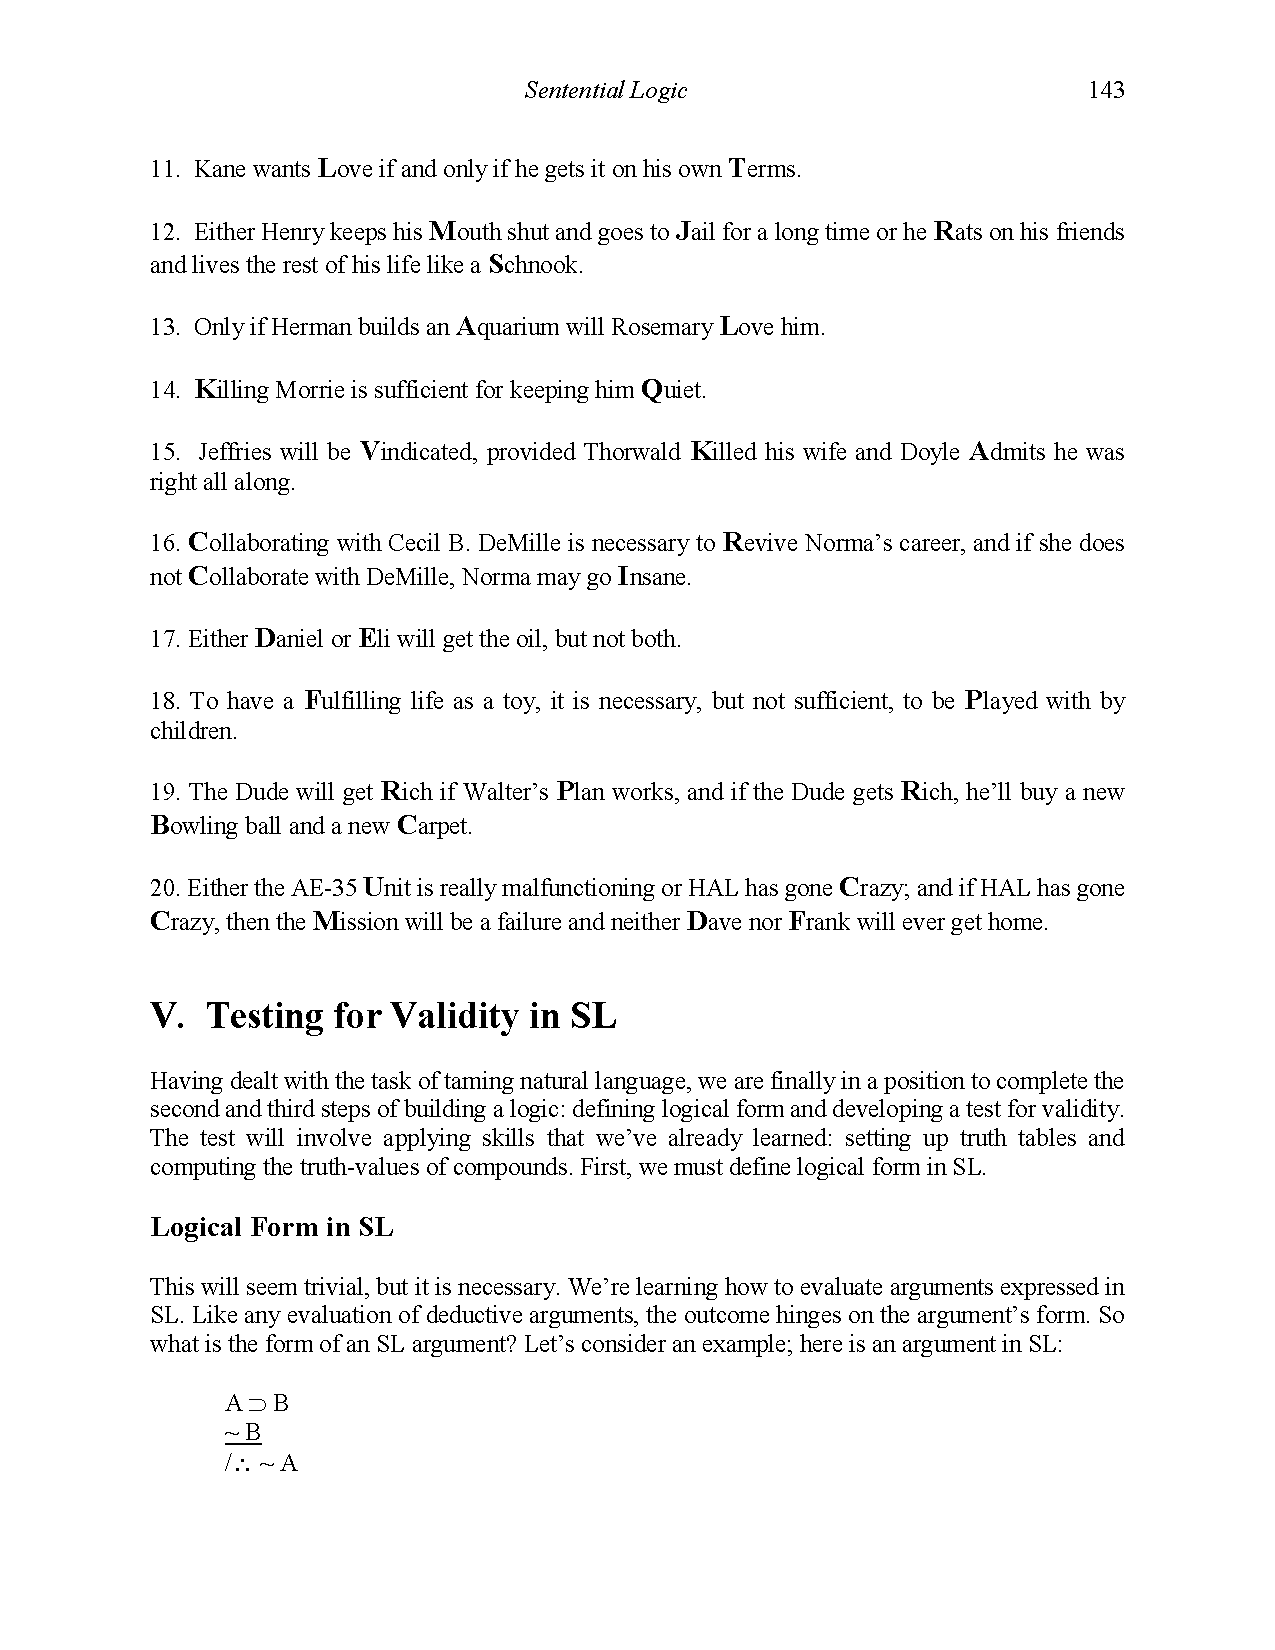
\includepdf[pages=-, pagecommand={}]{third.pdf}

%1
%\chapter{Chapter X}
% 





%\bibliography{humebib}
%\bibliography{humebib}
%\bibliographystyle{apalike}

\end{document}


